\chapter{Homological algebra}
\label{chap:homol}

The limited exposure to the Tor and Ext functors given in \ref{sec:linrep:tensor-products-and-the-tor-functors}
and \ref{sec:linrep:projective-and-injective-modules-and-the-ext-functors} should assist the reader in occasional encounters with
these functors. However, it is very worthwhile to go back, dotting all
i's and crossing all t's as necessary to prove the wonderful facts
responsible for the existence and the behavior of these functors. This
is one motivation for the material covered in this chapter. Tor and
Ext are examples of derived functors, a machinery that would give us
access to several other important constructions, such as group or
sheaf cohomology. Exploring any of these applications would take us
too far, but understanding the basics of homological algebra,
including a thorough look at derived functors, is in itself a very
worthwhile goal.  The material covered here should arm the reader with
enough information to be able to absorb any application quickly when
the time comes and the opportunity arises. All the wonderful mysteries
about Tor and Ext stated in \Cref{chap:linrep} will be recovered as very
particular cases of the results presented in this chapter.

The natural context in which to play this game is that of abelian
categories: these are categories carrying good notions of kernels and
cokernels, with properties to which the reader is accustomed due to
long exposure to the category $R\text{-}\categ{Mod}$ of modules over a
ring. In fact, elementary (and not so elementary) presentations of
homological algebra often take the standpoint that one may as well
work with $R\text{-}\categ{Mod}$; allegedly, nothing of substance is
lost by doing this rather than trying to work in the more natural
context of abelian categories.  I am not completely convinced. This
pedagogical device has strong theoretical backing, provided by the
Freyd--Mitchell embedding theorem: every small abelian category is
equivalent to a full subcategory of the category of left-modules over
a (not necessarily commutative) ring.  However, I believe that some
exposure to purely `arrow-theoretic' arguments is intrinsically
beneficial, and the reader should have the chance to acquire a taste
for this type of reasoning. In any case, I dislike the idea of simply
asking the reader to believe that `most of what follows works in a
more general setting', without providing some evidence for this fact.
Therefore, we will take a little time to look at abelian categories
before getting into homological algebra proper; this will be done in
the first two sections of this chapter, which an impatient reader
could probably skip over without much harm. While we will not prove
the Freyd--Mitchell embedding theorem, I will give a solid
justification for the fact that we can indeed perform diagram chases
by working with `elements', in the sense of (for example) checking
whether a diagram is commutative or whether a given sequence is exact.
Proving this will give us good practice in maneuvering arrow-theoretic
arguments; once we are done with it, we can indeed develop homological
algebra using conventional `element-theoretic' arguments, with a
relatively clean conscience.  As for homological algebra proper, my
general guiding principle will be to hunt for the `essence of
(co)homology': what information in a complex (see \ref{sec:rings:complexes-and-homology}) is really
responsible for its homology. This will motivate most constructions in
this chapter, including derived functors. A guiding beacon throughout
the chapter will be the notion of derived category: I will not
construct derived categories in full generality, but the reader should
nevertheless emerge with a basic understanding of what they are. One
reason for this compromise is that I felt that delving into
triangulated categories would take us too far; they are only mentioned
in passing at the end of the chapter.  Balancing Tor and Ext will
motivate the introduction of double complexes, and these in turn will
motivate a quick treatment of spectral sequences, in the last section.

\section{(Un)necessary categorical preliminaries}
\label{sec:homol:un-necessary-categorical-preliminaries}


\subsection{Undesirable features of otherwise reasonable categories}
\label{subsec:homol:undesirable-features-of-otherwise-reasonable-categories}
The category of modules over a ring $R$ is the template example of an
abelian category: a category for which it makes sense to talk about
`kernels' and `cokernels', `complexes', `exactness', etc., and in
which convenient results such as the `snake lemma' hold. We begin by
trying to concretize these thoughts a little.  As motivation for the
key definitions, I will first list a few annoying features of some of
the categories we have encountered.
\begin{itemize}
\item A category may not have initial or final objects; even if they
  are there, they may not be the same objects (as in $\categ{Set}$).
\item Products, coproducts may not exist (if the product of
  $\mathbb{F}_2$ and $\mathbb{F}_3$ existed in $\categ{Fld}$, what
  would its characteristic be?).
\item It may make no sense to talk about kernels and cokernels in a
  category; even when it does make sense, they may not exist (kernels
  do not necessarily exist in the category of finitely generated
  modules over a ring; cf.\ \Cref{exam:rings:infinite-poly-ring-fg}).
\item Even when there are kernels and cokernels, monomorphisms need
  not be kernels (nonnormal subgroups are not kernels: remember
  \ref{subsec:groups:kernel-iff-normal}), and epimorphisms need not be cokernels (the injection
  $\Z \to \Q$ is an epimorphism in $\categ{Ring}$; see \ref{subsec:rings:monomorphisms-and-epimorphisms}).
\item A morphism may be a monomorphism and an epimorphism without
  being an isomorphism ($\categ{Ring}$ again, same example).
\end{itemize}
Homological algebra will deal extensively with kernels, cokernels,
exact sequences, and the like: the material covered in \ref{sec:rings:complexes-and-homology} will
be our starting point. That material was developed for the category
$R\text{-}\categ{Mod}$ of (left-)modules over a ring, for which none
of the annoying things listed above occurs: in $R\text{-}\categ{Mod}$
every epimorphism is a cokernel, a map is an isomorphism if and only
if it is a monomorphism and an epimorphism, there is a zero-object
($=$ both initial and final), and so on.  The notions of `additive'
and `abelian' category extract the few key properties that guarantee
that no pathologies such as those listed above may occur. Working in
such categories `feels' quite a bit like working in
$R\text{-}\categ{Mod}$, in the sense that all expected properties of
kernels and cokernels hold. The Freyd--Mitchell embedding theorem (see
\S{}2.4) will provide a mathematical reason supporting this
psychological fact.

\subsection{Additive categories}
\label{subsec:homol:additive-categories}

\begin{defn}{}{homol:1.1}
  A category $\categ{A}$ is \emph{additive} if it has a zero-object,
  $\categ{A}$ has both finite products and finite coproducts, and each
  set of morphisms $\mathrm{Hom}_{\categ{A}}(A, B)$ is endowed with an
  abelian group structure, in such a way that the composition maps are
  bilinear. A functor between two additive categories is
  \emph{additive} if it preserves the abelian group structures on
  Hom-sets.
\end{defn}
None of the categories mentioned in the list in \S{}1.1 is additive.
Even $\categ{Grp}$ (which has kernels and cokernels, products, etc.)
is not an additive category: the Hom-sets in $\categ{Grp}$ do not have
a natural abelian group structure. Of course $\categ{Ab}$ is additive,
and so are all categories $R\text{-}\categ{Mod}$.  If a category
$\categ{A}$ is additive, it makes sense to talk about `zero-morphisms'
(which I will denote by $0$) and to add or subtract morphisms; two
morphisms $\alpha$, $\beta$ are equal if and only if
$\alpha - \beta = 0$. One can also talk about kernels and cokernels in
$\categ{A}$, by adopting the categorical definitions as suitable
limits and colimits (\Cref{linrep:exam:1.11}). Here are those definitions
again, expanded for intelligibility:
\begin{defn}{}{homol:1.2}
  Let $\varphi : A \to B$ be a morphism in an additive category
  $\categ{A}$. A morphism $\iota : K \to A$ is a \emph{kernel} of
  $\varphi$ if $\varphi \circ \iota = 0$ and for all morphisms
  $\zeta : Z \to A$ such that $\varphi \circ \zeta = 0$ there exists a
  unique $\tilde\zeta : Z \to K$ making the diagram
  \[\begin{tikzcd}
      Z \arrow[rr, "0", bend left=40] \arrow[r, "\zeta"] \arrow[d,
      dashed, "\exists! \, \tilde\zeta"'] &
      A \arrow[r, "\varphi"] & B \\
      K \arrow[ur, "\iota"']
    \end{tikzcd}\] commute. A morphism $\pi : B \to C$ is a
  \emph{cokernel} of $\varphi$ if $\pi \circ \varphi = 0$ and for all
  morphisms $\beta : B \to Z$ such that $\beta \circ \varphi = 0$
  there exists a unique $\tilde\beta : C \to Z$ making the diagram
  \[\begin{tikzcd}
      A \arrow[r, "\varphi"] \arrow[rrd, "0"', bend right=20] & B
      \arrow[r, "\pi"] \arrow[dr, "\beta"'] &
      C \arrow[d, dashed, "\exists! \, \tilde\beta"] \\
      & & Z
    \end{tikzcd}\] commute.
\end{defn}

Here is the same in sound-bite format: if $\varphi \circ \zeta = 0$,
then $\zeta$ factors uniquely through $\ker\varphi$. If
$\beta \circ \varphi = 0$, then $\beta$ factors uniquely through
$\coker\varphi$.  We have to get used to the fact that
morphisms may have `many' kernels (or cokernels), uniquely identified
with each other by virtue of being answers to a universal question
(\Cref{prop:prelims:initial-final-unique}); it is common to harmlessly abuse language and
talk about the kernel and the cokernel of a morphism. Further, we have
to get used to the fact that the kernel $\iota : K \to A$ of a
morphism $A \to B$ is a morphism. In a category such as $\categ{Ab}$
we are used to thinking of the kernel as a subobject of $A$, but this
is really nothing but the datum of an inclusion map: the kernel is
really that map. In an arbitrary category one cannot talk about
`subobjects' or `inclusions'; the closest one can get to these notions
is monomorphism. Similarly, `surjective' is not really an option;
epimorphism is the appropriate replacement. Recall (\ref{subsec:prelims:functions:monomorphisms-and-epimorphisms}) that
$\varphi : A \to B$ is a monomorphism if for all parallel morphisms
$\zeta_1, \zeta_2 : Z \to A$,
\[
  Z \xrightarrow[\zeta_2]{\zeta_1} A \xrightarrow{\varphi} B,
\]
$\varphi \circ \zeta_1 = \varphi \circ \zeta_2 \implies \zeta_1 =
\zeta_2$. It is an epimorphism if for all parallel
$\beta_1, \beta_2 : B \to Z$,
% A
\[
  A \xrightarrow{\varphi} B \xrightarrow[\beta_2]{\beta_1} Z,
\]
$\beta_1 \circ \varphi = \beta_2 \circ \varphi \implies \beta_1 =
\beta_2$. One benefit of working in an additive category is that these
definitions simplify a little:
\begin{lem}{}{homol:1.3}
  A morphism $\varphi : A \to B$ in an additive category is a
  monomorphism if and only if for all $\zeta : Z \to A$,
  \[
    \varphi \circ \zeta = 0 \implies \zeta = 0.
  \]
  It is an epimorphism if and only if for all $\beta : B \to Z$,
  \[
    \beta \circ \varphi = 0 \implies \beta = 0.
  \]
\end{lem}
\begin{proof}
  This is simply because two morphisms with the same source and target
  are equal if and only if their difference in the corresponding
  Hom-set (which is an abelian group by hypothesis) is $0$.
\end{proof}

Are kernels necessarily monomorphisms? Yes:
\begin{lem}{}{homol:1.4}
  In any additive category, kernels are monomorphisms and cokernels
  are epimorphisms.
\end{lem}
We will run into several such `dual' statements, and I will give the
proof for one half, leaving the other half to the reader; as a rule,
the two proofs mirror each other closely. There is a good reason for
this: the opposite (cf.\ \Cref{exer:3.1}) of an additive category is
additive, and kernels, monomorphisms, etc., in one correspond to
cokernels, epimorphisms, etc., in the other. Thus, proving one of
these statements for all additive categories establishes at the same
time the truth of its dual statement.  However, going through the
motions necessary to produce stand-alone proofs of the dual statements
makes for good practice, and I invite the reader to work out the
corresponding exercises at the end of this section. It is invariably
the case that these arguments are relatively easy to understand and
picture in one's mind but rather awkward to write down precisely. This
seems to be a feature of many arrow-theoretic arguments and probably
reflects inveterate biases acquired by early exposure to
$\categ{Set}$.
\begin{proof}
  Let $\varphi : A \to B$ be a morphism in an additive category
  $\categ{A}$, and let $\coker\varphi : B \to C$ be its
  cokernel. Let $\gamma : C \to Z$ be a morphism such that
  $\gamma \circ \coker\varphi = 0$. The composition
  $(\gamma \circ \coker\varphi) \circ \varphi$ is $0$;
  by definition of cokernel,
  $\gamma \circ \coker\varphi$ factors uniquely through
  $C$:
  \[\begin{tikzcd}
      A \arrow[r, "\varphi"] & B \arrow[r, "\gamma \circ
      \coker\varphi = 0"]
      \arrow[d, "\coker\varphi"'] & Z \\
      & C \arrow[ur, dashed, "\gamma"', "\exists!"']
    \end{tikzcd}\] Since
  $\gamma \circ \coker\varphi = 0 = 0 \circ
  \coker\varphi$, the uniqueness forces $\gamma = 0$.
  This proves that $\coker\varphi$ is an epimorphism, by
  Lemma~\ref{homol:1.3}.

  The proof that kernels are monomorphisms is analogous and is left to
  the reader (\Cref{exer:homol:1.9}).
\end{proof}
% ?
Certain limits are guaranteed to exist in an additive category: finite
products and coproducts do. On the other hand, kernels and cokernels
(which are also limits) do not necessarily exist in an additive
category. For example, the category of finitely generated modules over
a ring is additive, but it does not have kernels in general
(essentially because a submodule of a finitely generated module is not
necessarily finitely generated). But as soon as a morphism $\varphi$
does have kernels or cokernels in an additive category, the basic
qualities of that morphism can be detected `as usual' by looking at
$\ker\varphi$ and $\coker\varphi$. This is the case for
monomorphisms and epimorphisms:
\begin{lem}{}{homol:1.5}
  Let $\varphi : A \to B$ be a morphism in an additive category. Then
  $\varphi$ is a monomorphism if and only if $0 \to A$ is its kernel,
  and $\varphi$ is an epimorphism if and only if $B \to 0$ is its
  cokernel.
\end{lem}

Compare this statement with \Cref{prop:rings:kernels-cokernels}!

\begin{proof}
  Let's do kernels this time.  First assume $\varphi : A \to B$ is a
  monomorphism. If $\zeta : Z \to A$ is any morphism such that the
  composition $Z \to A \to B$ is $0$, then $\zeta$ is $0$ by
  Lemma~\ref{homol:1.3}, and in particular $\zeta$ factors (uniquely)
  through $0 \to A$. This proves that $0 \to A$ is a kernel of
  $\varphi$, as stated.  Conversely, assume that $0 \to A$ is a kernel
  for $\varphi : A \to B$, and let $\zeta : Z \to A$ be a morphism
  such that $\varphi \circ \zeta = 0$. It follows that $\zeta$ factors
  through $0 \to A$, since the latter is a kernel for $\varphi$:
  \[\begin{tikzcd}
      Z \arrow[rr, "0", bend left=40] \arrow[r, "\zeta"] \arrow[d,
      dashed, "\exists!"'] &
      A \arrow[r, "\varphi"] & B \\
      0 \arrow[ur]
    \end{tikzcd}\] This implies $\zeta = 0$, proving that $\varphi$ is
  a monomorphism.

  The statement about epimorphisms and cokernels is left to the reader
  (\Cref{exer:homol:1.9}).
\end{proof}
% ?
In view of Lemma~\ref{homol:1.5}, we should be able to use diagrams
\[
  0 \to A \to B, \quad A \to B \to 0
\]
to signal that $A \to B$ is a monomorphism, resp., an epimorphism:
think `exact'. However, the fact that kernels and cokernels do not
necessarily exist makes talking about exactness problematic in a
category that is `only' additive. This situation will be rectified
very soon.

Incidentally, it is common to denote monomorphisms and epimorphisms by
suitably decorated arrows; popular choices are $\rightarrowtail$ and
$\twoheadrightarrow$, respectively.

\subsection{Abelian categories}
\label{subsec:homol:abelian-categories}
The moral at this point is that if a morphism in an additive category
has kernels and cokernels, then these will behave as expected. But
kernels and cokernels do not necessarily exist, and this prevents us
from going much further. Also, while (as we have seen) kernels are
monomorphisms and cokernels are epimorphisms in an additive category,
there is no guarantee that monomorphisms should necessarily be kernels
and epimorphisms should be cokernels. In the end, we simply demand
these additional features explicitly.
\begin{defn}{}{homol:1.6}
  An additive category $\categ{A}$ is \emph{abelian} if kernels and
  cokernels exist in $\categ{A}$; every monomorphism is the kernel of
  some morphism; and every epimorphism is the cokernel of some
  morphism.
\end{defn}
% ?
As mentioned already, $R\text{-}\categ{Mod}$ is an abelian category,
for every ring $R$. The prototype of an abelian category is
$\categ{Ab}$: this\footnote{There is nothing particularly
  `commutative' about an abelian category.} is why these categories
are called abelian.  Since kernels are necessarily monomorphisms (by
Lemma~\ref{homol:1.4}), we see that in an \emph{abelian} category we
can adopt a mantra entirely analogous to the useful `kernel $\iff$
submodule' of \ref{subsec:rings:submodules-and-quotients} vintage: in abelian categories, the slogan
would be `kernel $\iff$ monomorphism' (and similarly for cokernels vs.
epimorphisms).
\begin{rem}{}{homol:1.7}
  Just as it is convenient to think of monomorphisms
  $A \rightarrowtail B$ as defining $A$ as a `subobject' of $B$, it is
  occasionally convenient to think of epimorphisms as `quotients': if
  $\varphi : A \rightarrowtail B$ is a monomorphism, we can use $B/A$
  to denote (the target of) $\coker\varphi$. We will
  have no real use for this notation in this section, but it will come
  in handy later on.
\end{rem}
The very existence of kernels and cokernels links these two notions
tightly in an abelian category:

\begin{lem}{}{homol:1.8}
  In an abelian category $\categ{A}$, every kernel is the kernel of
  its cokernel; every cokernel is the cokernel of its kernel.
\end{lem}

\begin{proof}
  I will prove the second half and leave the first half to the reader
  (\Cref{exer:homol:1.9}).

  Let $\varphi : A \to B$ be the cokernel of some morphism $Z \to A$;
  since $\categ{A}$ is abelian, $\varphi$ has a kernel
  $\iota : K \to A$. The composition $Z \to A \to B$ is $0$, so
  $Z \to A$ factors through $\iota$ by definition of kernel:
  \[\begin{tikzcd}
      Z \arrow[r] \arrow[d, dashed, "\exists!"'] &
      A \arrow[r, "\varphi"] & B \\
      K \arrow[ur, "\iota"']
    \end{tikzcd}\] Now let $A \to C$ be a morphism such that the
  composition $K \to A \to C$ is the zero-morphism; then so is the
  composition $Z \to A \to C$. Therefore $A \to C$ factors through a
  unique morphism $B \to C$,
  \[\begin{tikzcd}
      Z \arrow[r] \arrow[d, dashed, "\exists!"'] & A \arrow[r,
      "\varphi"] \arrow[rrd, near start] &
      B \arrow[dr, dashed, "\exists!"] & \\
      K \arrow[ur, "\iota"'] \arrow[rrr, "0"', bend right=20] & & & C
    \end{tikzcd}\] since $\varphi$ is the cokernel of $Z \to A$. But
  this shows that $\varphi : A \to B$ satisfies the property defining
  the cokernel of its kernel $K \to A$, as stated.
\end{proof}
% ?
Putting together Lemma~\ref{homol:1.8} and Lemma~\ref{homol:1.5}, we
can rephrase Definition~\ref{homol:1.6} by listing the following
requirements on a category $\categ{A}$:
\begin{itemize}
\item $\categ{A}$ is additive;
\item kernels and cokernels exist in $\categ{A}$;
\item if $\varphi : A \to B$ is a morphism whose kernel is $0$, then
  $\varphi$ is the kernel of its cokernel;
\item if $\psi : B \to C$ is a morphism whose cokernel is $0$, then
  $\psi$ is the cokernel of its kernel.
\end{itemize}
This is a popular equivalent reformulation of the definition of
abelian category. The last two requirements should call to mind the
exact sequence
\[
  0 \to A \xrightarrow{\varphi} B \xrightarrow{\psi} C \to 0
\]
familiar from the $R\text{-}\categ{Mod}$ context. The reader can
already entertain the sense in which such a sequence can be `exact' in
an abelian category: the third requirement identifies $A$ (or, rather,
$A \to B$) with the kernel of $\psi$, and the fourth one identifies
$C$ with the cokernel of $\varphi$.

Now suppose that $A \to B$ is sandwiched between zeros:
\[
  0 \to A \to B \to 0
\]
in an exact sequence. One of our many Pavlovian reactions would make
us want to deduce that $A \to B$ is an isomorphism, because this is
the case in $R\text{-}\categ{Mod}$, and this indeed works in any
abelian category:
\begin{lem}{}{homol:1.9}
  Let $\varphi : A \to B$ be a morphism in an abelian category
  $\categ{A}$, and assume that $\varphi$ is both a monomorphism and an
  epimorphism. Then $\varphi$ is an isomorphism.
\end{lem}

\begin{rem}{}{homol:1.10}
  This fact does not hold in general additive categories. In fact, the
  reader will encounter in \Cref{exer:homol:3.4} an example of an additive
  category with kernels and cokernels (but nevertheless not abelian)
  and with morphisms that are both monomorphisms and epimorphisms,
  without being isomorphisms.
\end{rem}
% ?
\begin{proof}
  By Lemma~\ref{homol:1.5} the kernel of $\varphi$ is $0 \to A$, since
  $\varphi$ is a monomorphism. Similarly, $B \to 0$ is a cokernel of
  $\varphi$. Further, $\varphi$ is the cokernel of $0 \to A$ and the
  kernel of $B \to 0$, by Lemma~\ref{homol:1.8}.

  Now consider the identity $B \to B$:
  \[\begin{tikzcd}
      & & B \arrow[d, "\id"] & \\
      0 \arrow[r] & A \arrow[r, "\varphi", tail, two heads] & B
      \arrow[r] & 0
    \end{tikzcd}\] Since $B \to B \to 0$ is (trivially) the zero
  morphism and $\varphi$ is the kernel of $B \to 0$, we obtain a
  unique morphism $\psi : B \to A$ making the diagram commute:
  \[\begin{tikzcd}
      & & B \arrow[d, "\id"] \arrow[dl, dashed, "\exists! \psi"'] & \\
      0 \arrow[r] & A \arrow[r, "\varphi", tail, two heads] & B
      \arrow[r] & 0
    \end{tikzcd}\]

  As $\varphi\psi = \id_B$, this shows that $\varphi$ has a
  right-inverse. Similarly, consider the identity $A \to A$, as
  follows:
  \[\begin{tikzcd}
      & A & & \\
      0 \arrow[r] & A \arrow[u, "\id"] \arrow[r, "\varphi",
      tail, two heads] & B \arrow[r] & 0
    \end{tikzcd}\]

  The composition $0 \to A \to A$ is the zero morphism, and $\varphi$
  is the cokernel of $0 \to A$, so we have a unique morphism
  $\eta : B \to A$ making this diagram commute:
  \[\begin{tikzcd}
      & A & & \\
      0 \arrow[r] & A \arrow[u, "\id"] \arrow[r, "\varphi",
      tail, two heads] & B \arrow[r] \arrow[ul, dashed, "\exists!
      \eta"'] & 0
    \end{tikzcd}\]

  This says $\eta\varphi = \id_A$, so $\varphi$ has a
  left-inverse as well.

  Thus, $\varphi$ has both a left-inverse $\eta$ and a right-inverse
  $\psi$. It follows that $\eta = \psi$ is a two-sided inverse of
  $\varphi$ and that $\varphi$ is an isomorphism as promised (cf.\
  \Cref{prop:prelims:iso-unique-inverse}).
\end{proof}
% ?
The reader should note the arrow-theoretic nature of this argument. In
the category $R\text{-}\categ{Mod}$ we could have given the following
(possibly) simpler argument: by \Cref{prop:rings:kernels-cokernels}, monomorphisms are
injective and epimorphisms are surjective; therefore $\varphi$ is
bijective, and bijective homomorphisms are isomorphisms by
\Cref{exer:rings:bijective-iso}. Such set-theoretic arguments are not an option in
an arbitrary abelian category (at least until we develop the material
of \S{}2), since the objects of an abelian category are not given as
`sets'. Judicious use of appropriate universal properties accomplishes
the same goal and may be argued to convey a `deeper' sense of why the
proven statement is true.

\subsection{Products, coproducts, and direct sums}
\label{subsec:homol:products-coproducts-and-direct-sums}
I will denote\footnote{As we will see, the single notation
  $A \oplus B$ will be an appropriate substitute for both notations.}
the product of two objects $A$, $B$ of an abelian category $\categ{A}$
by $A \times B$, and I will denote their coproduct by $A \sqcup
B$. Both exist, since $\categ{A}$ is additive.

The presence of these objects, and of kernels and cokernels, gives us
access to other interesting constructions.
\begin{exam}{}{homol:exam:1.11}
  For instance, fibered products (or `pull-backs') exist in any
  abelian category, just as in $R\text{-}\categ{Mod}$ (cf.\
  \Cref{exer:rings:fibered-product}). Consider a diagram
  \[\begin{tikzcd}
      & B \arrow[d, "\psi"] \\
      A \arrow[r, "\varphi"'] & C
    \end{tikzcd}\] in an abelian category. The fibered product of $A$
  and $B$ over $C$ is an object $A \times_C B$ with morphisms to $A$
  and $B$, completing the commutative diagram
  \[\begin{tikzcd}
      A \times_C B \arrow[r, "\varphi'"] \arrow[d, "\psi'"']
      \arrow[dr, phantom, "\lrcorner", very near start] &
      B \arrow[d, "\psi"] \\
      A \arrow[r, "\varphi"'] & C
    \end{tikzcd}\] and final with this property (that is what the
  small square in the middle of the diagram is supposed to
  indicate). The fibered product may be constructed in this context,
  just as in the particular case of $R\text{-}\categ{Mod}$, as the
  kernel of the difference of the two morphisms
  \[
    A \times B \xrightarrow[\varphi \circ \rho_A]{\psi \circ \rho_B}
    C,
  \]
  where $\rho_A, \rho_B$ are the morphisms making $A \times B$ a
  product. The reader will prove that these `fiber squares' preserve
  kernels, in the sense that $\ker\varphi = \psi' \circ \ker\varphi'$
  (\Cref{exer:homol:1.16}).

  Similarly, fibered coproducts (a.k.a.\ push-outs) may be constructed
  as cokernels of coproducts and preserve cokernels.
\end{exam}
In fact, in $R\text{-}\categ{Mod}$ such constructions are simplified
by the fact that finite products and coproducts coincide, in the sense
that the direct sum of two modules satisfies both universal
requirements for products and coproducts: \Cref{prop:rings:direct-sum-product-coproduct}. But the
direct sum of two modules $M_1$, $M_2$ is defined by giving a module
structure to the Cartesian product $M_1 \times M_2$. Again, this
strategy cannot be applied in a general abelian category, so we have
to come up with an alternative. This gives us another example of the
contrast between set-theoretic and arrow-theoretic arguments.  The
coproduct $A \sqcup B$ is endowed with morphisms
\[
  A \xrightarrow{i_A} A \sqcup B, \quad B \xrightarrow{i_B} A \sqcup
  B,
\]
which are easily checked to be monomorphisms (do this!). In an
arbitrary category, natural morphisms $A \sqcup B \to A$ and
$A \sqcup B \to B$ are not available (example: $\categ{Set}$).  In an
abelian category (and in fact already in an additive category) we do
have such morphisms: map $A \to A$ by the identity and $B \to A$ by
the zero-morphism to obtain a unique morphism
$\pi_A : A \sqcup B \to A$, making the following diagram commute:
\[\begin{tikzcd}
    A \arrow[r, "i_A"] \arrow[dr, "\id"'] &
    A \sqcup B \arrow[d, dashed, "\exists! \pi_A"] \\
    B \arrow[ur, "i_B"] \arrow[r, "0"'] & A
  \end{tikzcd}\] You can similarly define a morphism
$\pi_B : A \sqcup B \to B$. It follows (by the universal property of
products) that there is a unique morphism from $A \sqcup B$ to
$A \times B$ making the following diagram commute:
\[\begin{tikzcd}
    & A \\
    A \sqcup B \arrow[ur, "\pi_A"] \arrow[dr, "\pi_B"'] \arrow[r,
    dashed, "{\exists! \, (\pi_A, \pi_B)}"] &
    A \times B \arrow[u, "\rho_A"'] \arrow[d, "\rho_B"] \\
    & B
  \end{tikzcd}\] Now I claim that this morphism
$(\pi_A, \pi_B) : A \sqcup B \to A \times B$ is both a monomorphism
and an epimorphism. By Lemma~\ref{homol:1.9}, this (and a simple
induction) will prove

\begin{prop}{}{homol:1.12}
  In an abelian category, finite products and coproducts coincide.
\end{prop}

As it happens, this fact is already true in additive categories, and
the argument for this more general claim is (even) more
straightforward than what follows (\Cref{exer:homol:1.22}). Here I will prove
directly that the morphism $(\pi_A, \pi_B)$ is a monomorphism, leaving
to the reader the similar arguments needed to show that the same
morphism is an epimorphism. In the process, we recover for these
objects all the properties we expect on the basis of our experience
with $R\text{-}\categ{Mod}$.
\begin{itemize}
\item $\pi_B : A \sqcup B \to B$ is the cokernel of
  $i_A : A \to A \sqcup B$:

  Indeed, suppose $A \to A \sqcup B \to C$ is the zero-morphism; stare
  at
  \[\begin{tikzcd}
      A \arrow[r, "i_A"] & A \sqcup B \arrow[r, "\gamma"]
      \arrow[d, shift right, "\pi_B"'] & C \\
      & B \arrow[u, shift right, "i_B"'] \arrow[ur, "\gamma \circ
      i_B"'] &
    \end{tikzcd}\] and keep in mind that $\pi_B$ is determined by the
  requirements that $\pi_B \circ i_A = 0$ and
  $\pi_B \circ i_B = \id_B$.  We have to show that $\gamma$
  factors uniquely through $\pi_B$.  Note that if it factors at all,
  then the factorization is unique: indeed, if
  $\gamma = \delta \circ \pi_B$, then
  $\delta = \delta \circ (\pi_B \circ i_B) = (\delta \circ \pi_B)
  \circ i_B = \gamma \circ i_B$.  So the only morphism that can work
  is $\gamma \circ i_B$. Therefore, consider
  $(\gamma \circ i_B) \circ \pi_B$:
  \begin{itemize}
  \item
    $(\gamma \circ i_B) \circ \pi_B \circ i_A = 0 = \gamma \circ i_A$
    (since $\pi_B \circ i_A = 0$); and
  \item $(\gamma \circ i_B) \circ \pi_B \circ i_B = \gamma \circ i_B$
    (since $\pi_B \circ i_B = \id_B$).
  \end{itemize}
  By the universal property of coproducts, it follows that
  $(\gamma \circ i_B) \circ \pi_B = \gamma$, proving that $\gamma$
  indeed factors uniquely through $\pi_B$. This confirms that
  $\pi_B : A \sqcup B \to B$ is the cokernel of $i_A$.

\item $i_A : A \to A \sqcup B$ is the kernel of
  $\pi_B : A \sqcup B \to B$:

  Indeed, $i_A$ is a monomorphism since
  $A \xrightarrow{i_A} A \sqcup B \xrightarrow{\pi_A} A$ is the
  identity; hence it is a kernel (definition of abelian category!);
  hence it is the kernel of its cokernel (Lemma~\ref{homol:1.8}).

  By the same token, $\pi_A : A \sqcup B \to A$ is the cokernel of
  $i_B : B \to A \sqcup B$ and $i_B : B \to A \sqcup B$ is the kernel
  of $\pi_A : A \sqcup B \to A$.
\item The morphism $(\pi_A, \pi_B) : A \sqcup B \to A \times B$
  constructed above is a monomorphism:

  Consider the kernel $\iota$ of $(\pi_A, \pi_B)$. Composing with the
  projection to $B$ gives the zero-morphism:
  \[\begin{tikzcd}
      K \arrow[r, "\iota"] \arrow[rrr, "0"', bend right=20] & A \sqcup
      B \arrow[r, "{(\pi_A, \pi_B)}"] & A \times B \arrow[r, "\rho_B"]
      & B
    \end{tikzcd}\] It follows that $\iota$ factors through the kernel
  of $\pi_B$, that is, through $i_A$, and through $i_B$, by the same
  token.  Therefore we have the following commutative diagram:
  \[\begin{tikzcd}
      & A \arrow[d, "i_A"] & \\
      K \arrow[ur] \arrow[dr]' \arrow[r, "\iota"] &
      A \sqcup B \arrow[dr, "\pi_B"] & \\
      & B \arrow[u, "i_B"'] \arrow[r, "\id"'] & B
    \end{tikzcd}\] The composition $K \to A \to A \sqcup B \to B$ is
  zero (because $\pi_B \circ i_A = 0$); therefore so is the
  composition $K \to B \xrightarrow{\id} B$. That is,
  $K \to B$ is actually the zero-morphism; a fortiori, $\iota = 0$:
  the kernel of $A \sqcup B \to A \times B$ is $0$, so this morphism
  is indeed a monomorphism (by Lemma~\ref{homol:1.5}).
\end{itemize}

The same technique (or an appeal to the opposite category) proves that

\begin{itemize}
\item the morphism $(\pi_A, \pi_B) : A \sqcup B \to A \times B$
  constructed above is an epimorphism.
\end{itemize}

I will happily leave this to the reader (\Cref{exer:homol:1.17}).

This will conclude the proof of Proposition~\ref{homol:1.12}, by
Lemma~\ref{homol:1.9}.
% ?
In view of Proposition~\ref{homol:1.12}, we can adopt for any abelian
category $\categ{A}$ the convention of identifying $A \sqcup B$ and
$A \times B$, calling this object (defined up to isomorphism) the
\emph{direct sum} of $A$ and $B$, denoted $A \oplus B$. This object
comes endowed with natural morphisms
\[
  A \rightarrowtail A \oplus B, \quad B \rightarrowtail A \oplus B,
  \quad A \oplus B \twoheadrightarrow A, \quad A \oplus B
  \twoheadrightarrow B,
\]
satisfying all the properties to which we have grown accustomed.

\subsection{Images; canonical decomposition of morphisms}
\label{subsec:homol:images-canonical-decomposition-of-morphisms}
Yet another example of the application of an arrow-theoretic
perspective is the existence of `canonical decompositions' of
morphisms in any abelian category, in terms completely analogous to
the decompositions studied in $\categ{Set}$ (\ref{subsec:prelims:canonical-decomposition}), $\categ{Grp}$
(\ref{subsec:groups:canonical-decomposition}), $\categ{Ring}$ (\ref{subsec:rings:canonical-decomposition-and-consequences}), $R\text{-}\categ{Mod}$
(\ref{subsec:rings:canonical-decomposition-and-isomorphism-theorems}). In each of these previous examples we could simply
argue that the decomposition was the original decomposition obtained
in $\categ{Set}$, enriched as the case may be with additional
structures adapted to the category under examination. This is not an
option in the context of an abelian category, and yet the
decomposition holds just as well: every morphism may be written as an
epimorphism, followed by an isomorphism, followed by a monomorphism.
Here is the precise statement:
\begin{thm}{}{homol:1.13}
  Every morphism $\varphi : A \to B$ in an abelian category
  $\categ{A}$ may be decomposed as
  \[\begin{tikzcd}
      A \arrow[r, two heads] \arrow[rr, bend left, "\varphi"] & C
      \arrow[r, "\tilde{\varphi}", "\sim"'] & K \arrow[r, hook] & B
    \end{tikzcd}\] where $A \to C$ is the cokernel of the kernel of
  $\varphi$ and $K \to B$ is the kernel of the cokernel of
  $\varphi$. The induced morphism $\tilde{\varphi} : C \to K$ is
  uniquely determined and is an isomorphism.
\end{thm}
This theorem will follow from useful related considerations. Comparing
the statement with its set-theoretic counterpart suggests that
\[
  \ker(\coker\varphi) : \quad K \rightarrowtail B
\]
should play the role of the `image of $\varphi$'. Again note that the
set-theoretic definition of `image' is not an option in the general
context we are exploring: unlike groups, rings, etc., the objects of a
general abelian category are not `just' sets endowed with extra
structure.\footnote{However, we will soon recover a sense in which
  images in abelian categories can be `understood' in set-theoretic
  terms: see \Cref{homol:2.7}.} But look at your mental image of what the
image of a function $\varphi$ is; mine looks like this:
\begin{center}
  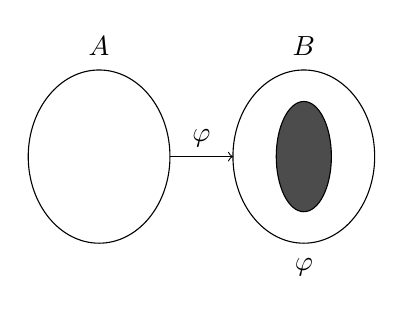
\begin{tikzpicture}[baseline=(current bounding box.center)]
    \draw (0,0) ellipse (0.9 and 1.1); \draw (2.6,0) ellipse (0.9 and
    1.1); \draw[fill=black!70] (2.6,0) ellipse (0.35 and 0.7);
    \draw[->] (0.9,0) -- (1.7,0) node[midway, above] {$\varphi$};
    \node at (0,1.4) {$A$}; \node at (2.6,1.4) {$B$}; \node at
    (2.6,-1.4) {$\image\varphi$};
  \end{tikzpicture}
\end{center}
We can fit many `subobjects' in $B$ to which $A$ maps via $\varphi$:
\begin{center}
  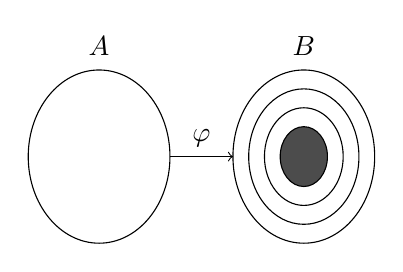
\begin{tikzpicture}[baseline=(current bounding box.center)]
    \draw (0,0) ellipse (0.9 and 1.1); \draw (2.6,0) ellipse (0.9 and
    1.1); \draw (2.6,0) ellipse (0.7 and 0.86); \draw (2.6,0) ellipse
    (0.5 and 0.62); \draw[fill=black!70] (2.6,0) ellipse (0.3 and
    0.38); \draw[->] (0.9,0) -- (1.7,0) node[midway, above]
    {$\varphi$}; \node at (0,1.4) {$A$}; \node at (2.6,1.4) {$B$};
  \end{tikzpicture}
\end{center}
and $\image\varphi$ is the `smallest' such subobject; that
is, it is initial with the property of being a subobject of $B$
through which $\varphi$ factors. This intuition is precisely captured
by $\ker(\coker\varphi)$, once we adapt to thinking of
`subobjects' as `monomorphisms':
\begin{lem}{}{homol:1.14}
  Let $\varphi : A \to B$ be a morphism in an abelian category, and
  let $\iota : K \to B$ be the kernel of the cokernel of $\varphi$.
  Then
  \begin{itemize}
  \item $\iota$ is a monomorphism;
  \item $\varphi$ factors through $\iota$; and
  \item $\iota$ is initial with these properties.
  \end{itemize}
\end{lem}

By Lemma~\ref{homol:1.4}, $\iota$ is a monomorphism. It is clear that
$\varphi$ factors through $\iota$: the composition
$A \to B \to \coker\varphi$ is the zero-morphism, so
there is a naturally induced $A \to K$ by the universal property of
kernels. The more interesting part of the statement of \Cref{homol:1.14}
asserts that if $\lambda : L \rightarrowtail B$ is any monomorphism
through which $\varphi$ also factors, then $\iota$ must factor
uniquely through $\lambda$:
\[\begin{tikzcd}
    & L \arrow[dr, hook, "\lambda"] & \\
    A \arrow[r] \arrow[rr, bend right, "\varphi"'] & K \arrow[u,
    dashed, "\exists!"] \arrow[r, hook, "\iota"'] & B
  \end{tikzcd}\]
\begin{proof}
  Consider $\coker\lambda$:
  \[\begin{tikzcd}
      & L \arrow[dr, "\lambda"] & \\
      A \arrow[ur] \arrow[r] & K \arrow[r, hook] &
      B \arrow[dr, "\coker\lambda"'] \\
      & & & \operatorname{Cok}\lambda
    \end{tikzcd}\] Since $\varphi$ factors through $\lambda$, the
  composition $A \to B \to \operatorname{Cok}\lambda$ is $0$; by the
  universal property of $\coker\varphi$, we have an
  induced map:
  \[\begin{tikzcd}
      & L \arrow[dr, "\lambda"] & & \\
      A \arrow[ur] \arrow[r] & K \arrow[r, hook] & B \arrow[r,
      "\coker\varphi"] \arrow[dr,
      "\coker\lambda"'] &
      \operatorname{Cok}_\varphi \arrow[d, dashed, "\exists!"] \\
      & & & \operatorname{Cok}\lambda
    \end{tikzcd}\] Since $K \to \operatorname{Cok}_\varphi$ is the
  zero-morphism, this implies that
  \[
    K \to B \xrightarrow{\coker\lambda}
    \operatorname{Cok}\lambda
  \]
  is the zero-morphism. Since $\lambda : L \to B$ is the kernel of its
  cokernel (Lemma~\ref{homol:1.8}), it follows that there is a unique
  morphism $K \to L$ making the diagram commute, as stated.
\end{proof}

\begin{defn}{}{homol:1.15}
  Let $\varphi : A \to B$ be a morphism in an abelian category. The
  \emph{image} of $\varphi$, denoted $\image\varphi$, is
  $\ker(\coker\varphi)$. The \emph{coimage} of
  $\varphi$, denoted $\operatorname{coim}\varphi$, is
  $\coker(\ker\varphi)$.
\end{defn}

Lemma~\ref{homol:1.14} motivates the first definition: every
monomorphism through which $\varphi$ factors must factor uniquely
through $\image\varphi$. (Of course in this context the
source of $\image\varphi$ is only defined up to (unique)
isomorphism, as is every solution to a universal problem.) As for the
second definition, the reader will formulate the universal property
satisfied by $\operatorname{coim}\varphi$ (\Cref{exer:homol:1.19}). With the
convention mentioned in \Cref{homol:1.7} and allowing for some abuse of
language, the (target of the) coimage of $\varphi : A \to B$ is the
`quotient' $A/\ker\varphi$.

My mental image, and surely yours, suggests that if $K \to B$ is the
image of $\varphi$, then the induced morphism
$\overline{\varphi} : A \to K$,
\[\begin{tikzcd}
    A \arrow[r, "\overline{\varphi}"] \arrow[rr, bend right,
    "\varphi"'] & K \arrow[r, hook] & B,
  \end{tikzcd}\] should be an epimorphism. This is indeed the case:
\begin{lem}{}{homol:1.16}
  Let $\varphi : A \to B$ be a morphism in an abelian category, and
  let $\image\varphi : K \to B$,
  $\operatorname{coim}\varphi : A \to C$ be its image and coimage,
  respectively. Then the induced morphisms $A \to K$ and $C \to B$
  are, respectively, an epimorphism and a monomorphism.
\end{lem}

\begin{proof}
  As usual, I will prove half of the statement and leave the other
  half to the reader (\Cref{exer:homol:1.20}.)

  To verify that $\overline{\varphi} : A \to K$ is an epimorphism,
  consider its image $K' \to K$:
  \[\begin{tikzcd}
      K' \arrow[r, hook, "\image\overline{\varphi} =
      \ker\coker\overline{\varphi}"] & K \arrow[r, two
      heads, "\coker\overline{\varphi}"] &
      \operatorname{Cok}.
    \end{tikzcd}\] Recall that every epimorphism is the cokernel of
  its kernel (Lemma~\ref{homol:1.8}); in particular,
  $\coker\overline{\varphi} =
  \coker(\image\overline{\varphi})$.  Now,
  $K' \to K$ is a monomorphism through which $\varphi$ factors:
  \[\begin{tikzcd}
      A \arrow[r] \arrow[rr, bend left, "\varphi"] & K' \arrow[r,
      hook, "\image\overline{\varphi}"] & K \arrow[r, hook]
      & B.
    \end{tikzcd}\] Therefore, $K' \to B$ is a monomorphism through
  which $\varphi$ factors and `preceding'
  $\image\varphi : K \to B$. Since the image of $\varphi$
  is initial among such morphisms (as proven in
  Lemma~\ref{homol:1.14}), necessarily
  $\image\overline{\varphi}$ is an isomorphism. It follows
  that
  $0 = \coker\image\overline{\varphi} =
  \coker\overline{\varphi}$, proving that
  $\overline{\varphi}$ is an epimorphism by Lemma~\ref{homol:1.5}.
\end{proof}
% ?
To summarize the situation, we have the following commutative diagram
of epimorphisms and monomorphisms factoring a given morphism $\varphi$
in an abelian category:
\[\begin{tikzcd}
    & K \arrow[dr, hook, "\image\varphi"] & \\
    A \arrow[ur, "\overline{\varphi}"] \arrow[rr, "\varphi"']
    \arrow[dr, two heads, "\operatorname{coim}\varphi"'] & & B. \\
    & C \arrow[ur, hook, "\underline{\varphi}"'] &
  \end{tikzcd}\]

Hopefully we have not lost track of our sought-for `canonical
decomposition':
\[
  \varphi : \quad
  \begin{tikzcd}
    A \arrow[r, two heads] & C \arrow[r, "\tilde{\varphi}", "\sim"'] &
    K \arrow[r, hook] & B.
  \end{tikzcd}
\]
We now see that this amounts to the statement that \emph{in an abelian
  category, there is an induced isomorphism linking the coimage and
  the image of every morphism.}

\begin{proof}[Proof of \cref{homol:1.13}]
  A unique morphism $\psi : K \to C$ making the above diagram commute
  exists, by the universal property of $\image\varphi$
  (Lemma~\ref{homol:1.14}), as well as by the universal property of
  $\operatorname{coim}\varphi$. Since
  $\underline{\varphi} \circ \psi = \image\varphi$ is a
  monomorphism, so is $\psi$. Since
  $\psi \circ \overline{\varphi} = \operatorname{coim}\varphi$ is an
  epimorphism, so is $\psi$. It follows that $\psi$ is an isomorphism
  (Lemma~\ref{homol:1.9}), and letting $\tilde{\varphi} : C \to K$ be
  the inverse of $\psi$ concludes the proof.
\end{proof}
Loosely speaking, we can say that, in an abelian category, `image and
coimage are naturally isomorphic'. This is imprecise, since image and
coimage are themselves morphisms; the isomorphism holds between the
target of coimage and the source of image. Of course, for friendly
categories such as $R\text{-}\categ{Mod}$ this distinction is
immaterial.

\subsection*{Exercises}

\begin{exer}{}{exer:homol:1.1}
  Prove that if $\psi \circ \varphi$ is an epimorphism, then $\psi$ is
  an epimorphism. Prove that if $\psi \circ \varphi$ is a
  monomorphism, then $\varphi$ is a monomorphism.
\end{exer}
\begin{exer}{}{exer:homol:1.2}
  Let $\varphi : A \to B$ be a morphism in an additive category. Prove
  that $-\varphi$ is a monomorphism, resp., epimorphism, if and only
  if $\varphi$ is.
\end{exer}
\begin{exer}{$\lnot$}{exer:homol:1.3}
  A \emph{preadditive} category is a category in which each Hom-set is
  endowed with an abelian group structure in such a way that
  composition maps are bilinear. Prove that a ring is `the same as' a
  preadditive category with a single object.

  Additive categories are preadditive categories with zero-objects and
  finite products and coproducts. Note that the notion of an `additive
  functor' between preadditive categories makes sense.  [\ref{exer:homol:1.12}]
\end{exer}
\begin{exer}{}{exer:homol:1.4}
  Let $\categ{A}$ be an additive category (preadditive would suffice),
  and let $A$ be an object of $\categ{A}$. Show that
  $\End_{\categ{A}}(A)$ has a natural ring structure.
\end{exer}
\begin{exer}{}{exer:homol:1.5}
  Let $A$, $B$ be objects of an additive category $\categ{A}$, with
  zero-object $0$. Since $0$ is both final and initial,
  $\Hom_{\categ{A}}(A,0)$ and $\Hom_{\categ{A}}(0,B)$ are both
  singletons, so the image of the composition
  \[
    A \to 0 \to B
  \]
  is a single element $e$ of $\Hom_{\categ{A}}(A,B)$.  Prove that this
  is the identity element of the abelian group
  $\Hom_{\categ{A}}(A,B)$. (Hint: Prove $e+e=e$.) In the text, this
  element is denoted $0$, the `zero-morphism'.

  Prove that for every morphism $\varphi$ in $\categ{A}$,
  $\varphi \circ 0 = 0 \circ \varphi = 0$.
\end{exer}
\begin{exer}{}{exer:homol:1.6}
  \exerused{} Prove that an object $A$ of an additive category
  $\categ{A}$ is a zero-object if and only if $\id_A$
  equals the zero-morphism $A \to A$. [\S{}\ref{subsec:homol:quasi-isomorphisms-and-derived-categories}]
\end{exer}
\begin{exer}{}{exer:homol:1.7}
  Give a categorical definition of cokernel in the spirit of the
  definition for kernel given in \Cref{linrep:exam:1.11}, and verify that
  the ordinary notion of cokernel in $R\text{-}\categ{Mod}$ satisfies
  this categorical requirement. Verify that your definition agrees
  with the one given in Definition~\ref{homol:1.2}.
\end{exer}
\begin{exer}{}{exer:homol:1.8}
  Let $\varphi : A \to B$ be a morphism in an additive category
  $\categ{A}$. Prove that $\iota : K \to A$ is a kernel for $\varphi$
  if and only if for all objects $Z$ the induced sequence
  \[\begin{tikzcd}
      0 \arrow[r] & \Hom_{\categ{A}}(Z,K) \arrow[r] &
      \Hom_{\categ{A}}(Z,A) \arrow[r] & \Hom_{\categ{A}}(Z,B)
    \end{tikzcd}\] is exact. Formulate an analogous result for
  cokernels.
\end{exer}
\begin{exer}{}{exer:homol:1.9}
  \exerused{} This exercise completes the proofs of results given in
  the text. The arguments should be constructed so as to mirror the
  proofs of the companion statements given in the quoted lemmas.

  Let $\categ{A}$ be an additive category.
  \begin{itemize}
  \item Let $\iota : K \to A$ be a kernel in $\categ{A}$; prove that
    $\iota$ is a monomorphism. (Cf.\ Lemma~\ref{homol:1.4}.)
  \item Let $\varphi : A \to B$ be a morphism in $\categ{A}$. If
    $\varphi$ has a cokernel, prove that $\varphi$ is an epimorphism
    if and only if $B \to 0$ is its cokernel. (Cf.\
    Lemma~\ref{homol:1.5}.)
  \item If $\categ{A}$ is abelian, prove that every kernel in
    $\categ{A}$ is the kernel of its cokernel. (Cf.\
    Lemma~\ref{homol:1.8}.)
  \end{itemize} [\S{}\ref{subsec:homol:abelian-categories}]
\end{exer}
\begin{exer}{}{exer:homol:1.10}
  \exerused{} Prove that the opposite $\categ{A}^{op}$ (cf.\
  \Cref{exer:3.1}) of an abelian category is an abelian category.
  [\S{}\ref{subsec:homol:complexes-of-projective-and-injective-objects}]
\end{exer}
\begin{exer}{$\lnot$}{exer:homol:1.11}
  Let $\categ{A}$ be an abelian category, and let $\categ{C}$ be any
  small category. Prove that the functor category
  $\categ{A}^{\categ{C}}$ (cf.\ \Cref{linrep:exer:1.9}) is an abelian
  category.

  For every object $X$ of $\categ{C}$, prove that the assignment
  $F \mapsto F(X)$ (with evident action on morphisms of
  $\categ{A}^{\categ{C}}$, i.e., natural transformations) determines
  an exact functor
  $\mathscr{X} : \categ{A}^{\categ{C}} \to \categ{A}$. [1.12, 1.14,
  1.15, 2.15, 5.7]
\end{exer}
\begin{exer}{}{exer:homol:1.12}
  For a ring $R$, let $\categ{R}$ denote the preadditive category with
  a single object determined by $R$ (\Cref{exer:homol:1.3}). Prove that the
  category $R\text{-}\categ{Mod}$ of left-$R$-modules is equivalent to
  the full subcategory consisting of additive functors in the functor
  category $\categ{Ab}^{\categ{R}}$ (cf.\ \Cref{exer:homol:1.11}). What about
  the category of right-$R$-modules?
\end{exer}
\begin{exer}{}{exer:homol:1.13}
  Let $R$ be a commutative ring, and let $R\text{-}\categ{Mod}^f$
  denote the category of finitely generated $R$-modules. Show that
  $R\text{-}\categ{Mod}^f$ need not be an abelian category; prove that
  it is, provided $R$ is Noetherian.
\end{exer}
\begin{exer}{}{exer:homol:1.14}
  Let $T$ be a topological space. Recall that a presheaf on $T$ with
  values in a category $\categ{A}$ is a contravariant functor from a
  certain category associated with $T$ to $\categ{A}$
  (\Cref{linrep:exam:1.5}). Define the \emph{category} of $\categ{A}$-valued
  presheaves on $T$. Prove that presheaves on $T$ with values in an
  abelian category form an abelian category. (Hint: \Cref{exer:homol:1.11}.)
\end{exer}
\begin{exer}{}{exer:homol:1.15}
  Consider the presheaf of continuous complex-valued functions
  $\mathscr{C}$ on a circle $S^1$ (cf.\ \Cref{linrep:exer:1.6}) and the
  presheaf $\mathscr{C}^*$ of continuous complex-valued functions that
  do not vanish anywhere along the circle; the first is a sheaf of
  abelian groups (under $+$), and so is the second (under $\cdot$).
  Use the exponential map to define a morphism
  $\exp : \mathscr{C} \to \mathscr{C}^*$.

  Prove that $\exp$ is \emph{not} an epimorphism of
  presheaves\footnote{Watch out! Both presheaves $\mathscr{C}$,
    $\mathscr{C}^*$ satisfy the \emph{sheaf} condition; cf.\
    \Cref{linrep:exer:1.6}. Sheaves of abelian groups form a full
    subcategory of the category of presheaves, and this category is
    also abelian, but the inclusion functor is in general \emph{not}
    exact. For example, the exponential map
    $\mathscr{C} \to \mathscr{C}^*$ considered above \emph{is} an
    epimorphism of sheaves.

    Also, for every open set $U$ of $T$, the assignment
    $F \mapsto F(U)$ defines a functor both on the category of
    presheaves of abelian groups and on the category of sheaves of
    abelian groups. This functor is exact on presheaves (this is a
    particular case of \Cref{exer:homol:1.11}), but the example given above
    shows that it is not exact in general on sheaves. This lack of
    exactness is responsible for the existence of sheaf cohomology.}:
  show that its cokernel has value $0$ over every proper open set of
  $S^1$ but is nonzero over $S^1$.
\end{exer}
\begin{exer}{}{exer:homol:1.16}
  \exerused{} Consider the pull-back diagram
  \[\begin{tikzcd}
      A \times_C B \arrow[r, "\varphi'"] \arrow[d, "\psi'"']
      \arrow[dr, phantom, "\lrcorner", very near start] &
      B \arrow[d, "\psi"] \\
      A \arrow[r, "\varphi"'] & C
    \end{tikzcd}\] in an abelian category; prove that the induced
  morphism from the source of $\ker\varphi'$ to the source of
  $\ker\varphi$ is an isomorphism.

  State and prove an analogous result for push-outs. [\S{}1.4,
  \S{}2.2, \S{}6.2]
\end{exer}
\begin{exer}{}{exer:homol:1.17}
  \exerused{} Prove that the morphism $A \amalg B \to A \times B$
  defined for objects $A$, $B$ of an abelian category is an
  epimorphism. [\S{}\ref{subsec:homol:products-coproducts-and-direct-sums}]
\end{exer}
\begin{exer}{}{exer:homol:1.18}
  Formulate a notion of `intersection' of two monomorphisms with a
  common target $A \rightarrowtail Z$, $B \rightarrowtail Z$ in an
  abelian category. Prove that the intersection of the natural
  monomorphisms $A \rightarrowtail A \oplus B$,
  $B \rightarrowtail A \oplus B$ is $0$.
\end{exer}
\begin{exer}{}{exer:homol:1.19}
  \exerused{} Formulate the universal property satisfied by the
  coimage of a morphism in an abelian category. [\S{}\ref{subsec:homol:images-canonical-decomposition-of-morphisms}]
\end{exer}
\begin{exer}{}{exer:homol:1.20}
  \exerused{} Let $A \to B$ be a morphism in an abelian category, with
  coimage $A \to C$, and let $C \to B$ be the induced morphism. Prove
  that $C \to B$ is a monomorphism. (Cf.\ Lemma~\ref{homol:1.16}; you
  should not use Theorem~\ref{homol:1.13}, since
  Lemma~\ref{homol:1.16} was used in its proof.) [\S{}\ref{subsec:homol:images-canonical-decomposition-of-morphisms}]
\end{exer}
\begin{exer}{$\lnot$}{exer:homol:1.21}
  Let $\varphi : A \to B$ be a morphism in an abelian category, and
  assume $\varphi$ decomposes as an epimorphism $\pi$ followed by a
  monomorphism $i$:
  \[\begin{tikzcd}
      A \arrow[r, two heads, "\pi"'] \arrow[rr, bend left, "\varphi"]
      & C \arrow[r, hook, "i"'] & B.
    \end{tikzcd}\] Prove that necessarily
  $\pi = \operatorname{coim}\varphi$ and
  $i = \image\varphi$. [\S{}\ref{subsec:homol:long-exact-sequence-of-derived-functors}]
\end{exer}
\begin{exer}{}{exer:homol:1.22}
  \exerused{} Prove that finite products and coproducts coincide in
  any \emph{additive} category. (Hint: To show that $A \amalg B$
  satisfies the universal property for $A \times B$, let
  $\alpha : C \to A$ and $\beta : C \to B$ be two morphisms, and
  define $C \to A \amalg B$ by $i_A \circ \alpha + i_B \circ \beta$.)
  [\S{}\ref{subsec:homol:products-coproducts-and-direct-sums}]
\end{exer}

\section{Working in abelian categories}
\label{sec:homol:working-in-abelian-categories}


\subsection{Exactness in abelian categories}
\label{subsec:homol:exactness-in-abelian-categories}
Now that we have a good notion of image in any abelian category, we
can formalize the meaning of `exact sequence'. Consider a sequence of
objects and morphisms in an abelian category:
\[\begin{tikzcd}
    \dots \arrow[r] & A \arrow[r, "\varphi"] & B \arrow[r, "\psi"] & C
    \arrow[r] & \dots.
  \end{tikzcd}\] The sequence is \emph{exact at $B$} if
\begin{enumerate}[label=(\arabic*)]
\item $\psi \circ \varphi = 0$ and
\item $\coker\varphi \circ \ker\psi = 0$.
\end{enumerate}
The first condition makes the sequence a `complex'; it tells us that
$\varphi$ factors through $\ker\psi$. As $\ker\psi$ is a monomorphism,
the universal property of images (Lemma~\ref{homol:1.14}) yields a
unique factorization of $\image\varphi$ through $\ker\psi$.
Similarly, the second condition tells us that $\ker\psi$ factors
through
$\ker(\coker\varphi) = \image\varphi$.  This
implies that $\image\varphi$ and $\ker\psi$ coincide.  The
conditions defining exactness can therefore be summarized as
\begin{itemize}
\item $\image\varphi = \ker\psi$.
\end{itemize}
Of course this recovers precisely the condition used to define the
notion of exactness of a sequence of $R$-modules, in \ref{subsec:rings:complexes-and-exact-sequences}. All
expected elementary connotations of exactness hold in the context of
abelian categories as in $R\text{-}\categ{Mod}$, as envisioned already
in \S{}1.2--1.3. With notation as above, if the sequence is exact at
$B$, then $\psi$ is a monomorphism if and only if $\varphi$ is the
zero-morphism, and $\varphi$ is an epimorphism if and only if $\psi$
is the zero-morphism; the sequence
\[\begin{tikzcd}
    0 \arrow[r] & A \arrow[r, "\varphi"] & B \arrow[r, "\psi"] & C
    \arrow[r] & 0
  \end{tikzcd}\] is exact if and only if $\varphi$ is a kernel of
$\psi$ and $\psi$ is a cokernel of $\varphi$, and
\[\begin{tikzcd}
    0 \arrow[r] & A \arrow[r, "\varphi"] & B \arrow[r] & 0
  \end{tikzcd}\] is exact if and only if $\varphi$ is an isomorphism.
\begin{exam}{}{homol:2.1}
  There is a natural exact sequence
  \[\begin{tikzcd}
      0 \arrow[r] & A \arrow[r] & A \oplus B \arrow[r] & B \arrow[r] &
      0
    \end{tikzcd}\] where $A \oplus B$ is the direct sum defined in
  \S{}1.4.
\end{exam}
\begin{exam}{}{homol:2.2}
  For a slightly more interesting example, consider a diagram
  \[\begin{tikzcd}
      D \arrow[r, "\varphi'"] \arrow[d, "\psi'"'] & B \arrow[d, "\psi"] \\
      A \arrow[r, "\varphi"'] & C
    \end{tikzcd}\] and the associated sequence
  \[\begin{tikzcd}
      D \arrow[r, "{(\psi', \varphi')}"] & A \oplus B \arrow[r,
      "{(\varphi, -\psi)}"] & C
    \end{tikzcd}\] obtained by letting $A \oplus B$ play both roles of
  product and coproduct. Then
  \begin{itemize}
  \item the diagram is commutative if and only if this sequence is a
    complex;
  \item the sequence obtained by adding a $0$ to the left,
    \[\begin{tikzcd}
        0 \arrow[r] & D \arrow[r] & A \oplus B \arrow[r] & C,
      \end{tikzcd}\] is exact if and only if $D$ may be identified
    with the fibered product $A \times_C B$ (cf.\
    Example~\ref{homol:exam:1.11});
  \item likewise, the sequence
    \[\begin{tikzcd}
        D \arrow[r] & A \oplus B \arrow[r] & C \arrow[r] & 0
      \end{tikzcd}\] is exact if and only if $C$ may be identified
    with the fibered coproduct $A \amalg_D B$.
  \end{itemize}
  Indeed, the first assertion is trivial; the second and third amount
  to the explicit construction of fibered products and coproducts
  mentioned in Example~\ref{homol:exam:1.11}.
\end{exam}

\subsection{The snake lemma, again}
\label{subsec:homol:the-snake-lemma-again}
The reader is now in the position of making sense in any abelian
category of all the statements given in \ref{sec:rings:complexes-and-homology} for sequences of
$R$-modules; this includes the definition of the \emph{homology} of a
complex as a measure of the failure of exactness. These facts will be
reviewed in \S{}3. However, note that while we can now \emph{state}
the snake lemma (\Cref{lem:rings:snake-lemma}) in any abelian category, the (sketch
of the) \emph{proof} given in \ref{sec:rings:complexes-and-homology} cannot be directly lifted from
that context and applied to this one, or so it would seem, since the
definition of the `snaking' homomorphism $\delta$ given in \ref{sec:rings:complexes-and-homology}
makes use of `elements'. Barring more sophisticated alternatives, we
should provide an arrow-theoretic alternative for the definition of
$\delta$.

This is perhaps not completely immediate.

As practice, note the following:
\begin{lem}{}{homol:2.3}
  Let
  \[\begin{tikzcd}
      A \times_C B \arrow[r, "\varphi'"] \arrow[d, "\psi'"'] &
      B \arrow[d, "\psi"] \\
      A \arrow[r, "\varphi"'] & C
    \end{tikzcd}\] be a fibered diagram in an abelian category, and
  assume $\varphi$ is an epimorphism. Then $\varphi'$ is also an
  epimorphism.
\end{lem}

It takes seconds to realize that this is true in
$R\text{-}\categ{Mod}$, by chasing elements. An arrow-theoretic proof
is considerably subtler.

\begin{proof}
  First, observe that if $\varphi : A \to C$ is an epimorphism, so is
  the map $A \oplus B \to C$ considered in Example~\ref{homol:2.2}.
  Since epimorphisms are cokernels in an abelian category and
  cokernels are cokernels of their kernels (Lemma~\ref{homol:1.8}), we
  see that $A \oplus B \to C$ is the cokernel of the natural morphism
  \[
    A \times_C B \to A \oplus B.
  \]
  To prove that $\varphi'$ is an epimorphism, it suffices
  (Lemma~\ref{homol:1.3}) to show that if $\zeta : B \to Z$ is a
  morphism for which $\zeta \circ \varphi' = 0$, then $\zeta = 0$.

  For this, consider the morphism
  \[\begin{tikzcd}
      A \oplus B \arrow[r, "{(0,\zeta)}"] & Z
    \end{tikzcd}\] obtained by using the fact that $A \oplus B$ is a
  coproduct of $A$ and $B$. The composition
  \[
    A \times_C B \to A \oplus B \to Z
  \]
  agrees with $\zeta \circ \varphi'$, so it is the zero-morphism. By
  the universal property of cokernels, we have the factorization
  \[\begin{tikzcd}
      A \oplus B \arrow[r, "{(0,\zeta)}"] \arrow[d] & Z \\
      C \arrow[ur, dashed, "\zeta'"']
    \end{tikzcd}\] for a unique morphism $\zeta'$. By the
  commutativity of
  \[\begin{tikzcd}
      A \arrow[r] \arrow[dr, "\varphi"'] &
      A \oplus B \arrow[r, "{(0,\zeta)}"] & Z \\
      & C \arrow[ur, "\zeta'"'] &
    \end{tikzcd}\] we see that the composition
  $\zeta' \circ \varphi : A \to C \to Z$ is the zero-morphism. Since
  $\varphi$ is an epimorphism, it follows that $\zeta' = 0$. This
  implies that $(0,\zeta) : A \oplus B \to Z$ is the zero-morphism,
  and we are done: $\zeta = 0$ as promised.
\end{proof}

Here is a quicker proof (for those who have done their homework): if
$\varphi$ is an epimorphism, then $A \oplus B \to C$ is an
epimorphism, so the diagram is a push-out as well as a pull-back
(Example~\ref{homol:2.2}). By \Cref{exer:homol:1.16},
$\coker\varphi' = \coker\varphi = 0$;
therefore $\varphi'$ is an epimorphism. The reader should have no
difficulty now proving the statement dual to Lemma~\ref{homol:2.3},
for fibered coproducts (\Cref{exer:homol:2.2}).  Going back to the snake lemma,
start from a commutative diagram linking two exact sequences in an
abelian category:
\[\begin{tikzcd}
    0 \arrow[r] & L_1 \arrow[r, "\alpha_1"] \arrow[d, "\lambda"'] &
    M_1 \arrow[r, "\beta_1"] \arrow[d, "\mu"'] &
    N_1 \arrow[r] \arrow[d, "\nu"'] & 0 \\
    0 \arrow[r] & L_0 \arrow[r, "\alpha_0"'] & M_0 \arrow[r,
    "\beta_0"'] & N_0 \arrow[r] & 0
  \end{tikzcd}\] The main task is to construct a connecting
morphism\footnote{To avoid unbearably heavy notation, I will write
  $\ker\nu$, etc., for the \emph{source} of the morphism $\ker\nu$,
  etc.}  $\delta : \ker\nu \to \coker\lambda$; once this
is done, we should prove the exactness of the sequence displayed in
\Cref{lem:rings:snake-lemma}. I will leave this latter step to the more enterprising
reader (who may want to wait until we go through \S{}2.3).  The
enterprising reader should in fact try to construct $\delta$, as an
exercise in coming up with arrow-theoretic proofs replacing
well-understood element-theoretic arguments. Feel free to stop reading
here and resume when you have tried on your own.

The `problem' is that the universal properties of kernel and cokernel
would seem to guarantee the existence of morphisms \emph{to} $\ker\nu$
and \emph{from} $\coker\lambda$. There's the rub: how on
earth are we going to get a morphism \emph{from} $\ker\nu$ \emph{to}
$\coker\lambda$? (Last chance to try on your own!)

The answer is to view $\ker\nu$ as a cokernel and
$\coker\lambda$ as a kernel. This can be achieved by
constructing suitable pull-back, resp., push-out, diagrams:
\[\begin{tikzcd}
    M_1 \times_{N_1} (\ker\nu) \arrow[r, "\beta_1'"] \arrow[d] &
    \ker\nu \arrow[d] \\
    M_1 \arrow[r, "\beta_1"'] & N_1
  \end{tikzcd}\!, \qquad
  \begin{tikzcd}
    L_0 \arrow[r, "\alpha_0"] \arrow[d] & M_0 \arrow[d] \\
    \coker\lambda \arrow[r, "\alpha_0'"'] &
    (\coker\lambda) \amalg_{L_0} M_0.
  \end{tikzcd}\] By Lemma~\ref{homol:2.3}, $\beta_1'$ is an
epimorphism since $\beta_1$ is an epimorphism, and $\ker\beta_1$,
$\ker\beta_1'$ have matching sources by \Cref{exer:homol:1.16}. Analogous
(dual) statements hold for the second diagram (Exercises~2.2 and
1.16). Putting everything into one commutative diagram,
\[\begin{tikzcd}[column sep=small]
    0 \arrow[r] & L_1 \arrow[r, "\sigma"] \arrow[d, equal] & M_1
    \times_{N_1} (\ker\nu) \arrow[r, "\beta_1'"] \arrow[ddd,
    "\epsilon", bend left=25] &
    \ker\nu \arrow[r] \arrow[d] & 0 \\
    0 \arrow[r] & L_1 \arrow[r, "\alpha_1"'] \arrow[d, "\lambda"'] &
    M_1 \arrow[r, "\beta_1"'] \arrow[d, "\mu"'] &
    N_1 \arrow[r] \arrow[d, "\nu"'] & 0 \\
    0 \arrow[r] & L_0 \arrow[r, "\alpha_0"'] \arrow[d] & M_0 \arrow[r,
    "\beta_0"'] \arrow[d] &
    N_0 \arrow[r] \arrow[d, equal] & 0 \\
    0 \arrow[r] & \coker\lambda \arrow[r, "\alpha_0'"']
    & (\coker\lambda) \amalg_{L_0} M_0 \arrow[r,
    "\tau"'] & N_0 \arrow[r] & 0
  \end{tikzcd}\] has exact rows (not columns!). We get a morphism
\[
  \epsilon : M_1 \times_{N_1} (\ker\nu) \to
  (\coker\lambda) \amalg_{L_0} M_0.
\]
Note that
\[
  \epsilon \circ \sigma = 0, \qquad \tau \circ \epsilon = 0
\]
by the commutativity of the diagram: indeed, the compositions
$L_1 \to \coker\lambda$, $\ker\nu \to N_0$ are both
zero.  Since $\ker\nu$ plays the role of cokernel in the top row,
$\epsilon \circ \sigma = 0$ implies that $\epsilon$ must factor
through $\ker\nu$, giving a morphism
\[
  \epsilon' : \ker\nu \to (\coker\lambda) \amalg_{L_0}
  M_0.
\]
Since $\coker\lambda$ plays the role of kernel in the
bottom row and $\tau \circ \epsilon' : \ker\nu \to N_0$ is the
zero-morphism (because
$\tau \circ \epsilon' \circ \beta_1' = \tau \circ \epsilon = 0$ and
$\beta_1'$ is an epimorphism), $\epsilon'$ must factor through
$\coker\lambda$, finally yielding
\[
  \delta : \ker\nu \to \coker\lambda.
\]
Writing elements out, the reader can verify that this morphism
$\delta$ agrees with the connecting morphism $\delta$ defined in
\ref{subsec:rings:homology-and-the-snake-lemma}. Together with maps induced by simpler considerations, we
obtain the sequence of morphisms
\[\begin{tikzcd}[column sep=small]
    0 \arrow[r] & \ker\lambda \arrow[r] & \ker\mu \arrow[r] & \ker\nu
    \arrow[r, "\delta"] & \coker\lambda \arrow[r] &
    \coker\mu \arrow[r] & \coker\nu
    \arrow[r] & 0
  \end{tikzcd}\] in our abelian category. I should now recommend that
the reader prove the exactness of this sequence, by appropriate
arrow-theoretic arguments. This would be excellent practice for many
such facts that we will encounter when we finally do begin to develop
homological algebra.

However, assuming that we have already done this work in \ref{subsec:rings:homology-and-the-snake-lemma},
by chasing elements, is it really necessary to go back and redo it
with arrows, in order to check the exactness of the sequence in an
abelian category?

\subsection{Working with `elements' in a small abelian category}
\label{subsec:homol:working-with-elements-in-a-small-abelian-category}
My personal feeling is that arrow-theoretic arguments are invariably
more insightful than their element-theoretic counterparts, even if
they are `harder' as a rule. At the very least, they are more elegant:
for example, in the construction of the connecting morphism $\delta$
just given above, there was no need to verify that the result was
`well-defined', while this requires an argument in the set-theoretic
construction in \ref{subsec:rings:homology-and-the-snake-lemma}. Such issues are usually resolved once and
for all at the start, when the key universal properties are
established, and it is not necessary to belabor them later.  Still, it
is true that element-theoretic arguments are usually easier to
concoct. Lemma~\ref{homol:2.3} appears to be a good example: in terms
of elements the statement of this lemma is completely obvious, less so
from the diagrammatic point of view. \Cref{exer:homol:2.12} gives another
example: providing a purely arrow-theoretic proof of the innocent
result stated there is not so easy, while this result is essentially
immediate from a more mundane viewpoint. The reader could wonder
whether it may not `be enough' to prove such facts---for example,
check the commutativity of a diagram or the exactness of a
sequence---by simpler element-theoretic considerations.  This is
indeed the case. I will present a construction which would suffice
for, e.g., the purpose of completing the proof of the snake lemma by
chasing elements rather than arrows. I find this construction
instructive and pretty, so I will take the time to go through it in
some detail. However, be warned that the Freyd--Mitchell embedding
theorem (discussed in \S{}2.4) will obliterate the actual usefulness
of the construction, since it provides us with a much stronger result.
Thus, I will ask the reader to wade through some material, with the
understanding that the result that I will quote thereafter
(\Cref{homol:2.9}) will make that material immediately obsolete.

My excuse is that while proving \Cref{homol:2.9} is beyond the scope of
this book, the construction which I am about to describe is entirely
within our reach, and good propaganda for the philosophy underlying
the functor of points; this is important in, e.g., algebraic geometry
and takes some practice to get used to. In the end, the reader is
likely to gain a better understanding of the situation by appreciating
a weaker result that we can prove entirely than by leaning on a
stronger result to be taken on faith. However, the hurried reader
should feel free to skip this material and jump directly to \S{}2.4.
The idea is to define an appropriate notion of an `element' of an
object of an abelian category.\footnote{I will systematically put
  quotes around this term, i.e., write `element', to indicate that I
  am referring to the relatively fancy notion I will introduce. The
  `elements' will be ordinary elements of an ordinary (pointed) set
  determined by the object of the category.} The reader should look
back at the brief discussion at the end of \ref{subsec:linrep:examples-of-functors}: the `functor
of points' $h_A = \Hom_{\categ{A}}(\_, A)$ associates to every object
$Z$ the set of morphisms $Z \to A$; in several categories, applying
this functor to a final object in $\categ{A}$ `recovers' $A$ as a
set. Working with final objects with this purpose cannot work too well
in categories with zero-objects (why?), but the idea underlying the
functor of points suggests that we look at morphisms
\[
  z : Z \to A
\]
for a fixed object $A$ in an abelian category $\categ{A}$ as
($Z$-flavored?!) `elements' $z$ of $A$.

If $\varphi : A \to B$ is a morphism in $\categ{A}$, it makes sense to
talk about the `element' $\varphi(z)$ of $B$: simply compose
morphisms, i.e.,
\[\begin{tikzcd}
    & Z \arrow[d, "z"'] \arrow[dr, "\varphi(z) = \varphi \circ z"] & \\
    & A \arrow[r, "\varphi"'] & B
  \end{tikzcd}\]

It would now be nice if one could simply check the commutativity of a
diagram in $\categ{A}$ or the exactness of a sequence by using these
newly defined `elements' as if they were elements of objects in
$\categ{A}$. This does not quite work: for example, the simple-minded
statement of surjectivity at the level of these `elements' is not
equivalent to the notion of epimorphism in $\categ{A}$. Indeed, if
$\varphi : A \to B$ is an epimorphism, it is not necessarily the case
that `for all elements $z$ of $B$ there exists an element $z'$ of $A$
such that $z = \varphi(z')$': this would amount to saying that every
morphism $z : Z \to B$ can be lifted to a morphism $z' : Z \to A$,
\[\begin{tikzcd}
    & A \arrow[d, "\varphi"] \\
    Z \arrow[ur, dashed, "\exists z'?"] \arrow[r, "z"'] & B
  \end{tikzcd}\] and this is simply not true in general (for example,
in $\categ{Ab}$ one cannot lift the identity $\Z/2\Z \to \Z/2\Z$ along
the projection $\Z \to \Z/2\Z$). The problem is really that $\Hom$ is
not right-exact, so it does not preserve epimorphisms.

Maybe surprisingly, there is a way to fix this problem.  As a
preliminary note, recall that in the distant past (\Cref{exam:prelims:pointed-sets}) we
considered the category $\categ{Set}^*$ of `pointed sets', whose
objects consist of sets endowed with the choice of a distinguished
point (here I will denote by $0$ the distinguished point). All the
algebraic structures we have encountered are pointed sets, often in
more than one way: for example, stripping an abelian group of all its
structure except its supporting set and the choice of the identity
element leaves us with a pointed set (in other words, this defines an
evident forgetful functor $\categ{Ab} \to \categ{Set}^*$).

The category $\categ{Set}^*$ has a zero-object $0$ (the singleton
$\{0\}$); hence we can talk of `zero-morphisms' in $\categ{Set}^*$.
Further, the category $\categ{Set}^*$ has enough structure to make
sense of the notion of an `exact sequence of pointed sets': we can
stipulate that
\[\begin{tikzcd}
    \dots \arrow[r] & S \arrow[r, "f"] & T \arrow[r, "g"] & U
    \arrow[r] & \dots
  \end{tikzcd}\] is `exact' at $T$ if the (set-theoretic!) image of
$f$ equals the `kernel' of $g$ (that is, the preimage
$g^{-1}(0)$). This notion should be taken with a grain of salt: while
it is the case that $S \to T \to 0$ is exact at $T$ if and only if
$S \to T$ is surjective, it is not true that $0 \to T \to U$ is exact
at $T$ in $\categ{Set}^*$ if and only if $T \to U$ is injective (the
only requirement posed by the exactness of $0 \to T \to U$ is that the
only element of $T$ mapping to the distinguished element in $U$ is the
distinguished element of $T$; this is weaker than injectivity). The
category $\categ{Set}^*$ is, after all, not additive.  Now we are
going to associate to every object $A$ of a (small) abelian category
$\categ{A}$ a pointed set $\hat{A}$. This will in fact give a functor
$\categ{A} \to \categ{Set}^*$ with amazing properties: a morphism will
be a monomorphism, resp., an epimorphism, in $\categ{A}$ if and only
if the corresponding function of pointed sets is injective, resp.,
surjective; the (arrow-theoretic) notions of kernel and image in
$\categ{A}$ will correspond precisely to the (set-theoretic) kernel
and image in $\categ{Set}^*$; a sequence of objects in $\categ{A}$
will be exact if and only if the corresponding sequence of pointed
sets is exact; and it will be possible to verify whether a diagram
commutes in $\categ{A}$ by working in $\categ{Set}^*$.

The upshot will be that in a sense we can chase a diagram in any small
abelian category by `chasing elements'. For example, working with
`elements' suffices to complete the proof of the snake lemma, in the
sense that the exactness (in $\categ{A}$) of the sequence obtained
with the aid of the connecting morphism defined in \S{}2.2 may be
verified by chasing `elements', since this verifies exactness in
$\categ{Set}^*$. A proof in $R\text{-}\categ{Mod}$ would transfer
word-for-word to give a proof in any small\footnote{If the relevant
  diagrams only involve finitely many objects, the smallness
  hypothesis is not restrictive. The interested reader should research
  this issue; I will shamelessly gloss over it.} abelian
category. This hints that the arrow-theoretic viewpoint that I have
tried to defend in the past several subsections, while elegant, is not
really strictly necessary; I will come back to this point in \S{}2.4.
The construction can be given as an application of the abstract
language developed in \ref{sec:linrep:preliminaries-reprise}; but I promise that the resulting
notion will be easy to contemplate, independently of this language.
The idea is simply to take the functor of points up to a relation
identifying the `element' $Z \to A$ with all `elements'
$W \twoheadrightarrow Z \to A$.

The following abstract nonsense will have a simple-minded explanation.
I will (often silently) assume that $\categ{A}$ is small, to steer
clear of any possible set-theoretic subtlety. It is convenient to
consider a companion category $\categ{A}_{\leftarrow}$, with the same
objects as $\categ{A}$ but in which
\[
  \Hom_{\categ{A}_{\leftarrow}}(Z,W) = \{\text{epimorphisms } W
  \twoheadrightarrow Z \text{ in } \categ{A}\}.
\]
This is legal, because the composition of two epimorphisms in
$\categ{A}$ is an epimorphism; but note that $\categ{A}_{\leftarrow}$
is no longer additive (the sum of two epimorphisms need not be an
epimorphism, so we lose the algebraic structure on Hom). Also note the
reversing of arrows; this is in order that the functor that I am about
to define be covariant.

I will use $\categ{A}_{\leftarrow}$ as `index' category for a limit.
For a fixed object $A$ of $\categ{A}$, I define a covariant functor
\[
  \mathscr{H}_A : \categ{A}_{\leftarrow} \to \categ{Set}^*
\]
by `restricting' the functor of points $h_A$ to
$\categ{A}_{\leftarrow}$ and preserving the information of the
zero-morphism. That is, I set
\[
  \mathscr{H}_A(Z) = \Hom_{\categ{A}}(Z,A)
\]
for all objects $Z$ of $\categ{A}_{\leftarrow}$ (that is, of
$\categ{A}$), viewing $\Hom_{\categ{A}}(Z,A)$ as a pointed set by
distinguishing the zero-morphism, and define $\mathscr{H}_A$ on
morphisms by composition: for a morphism $Z \to W$ in
$\categ{A}_{\leftarrow}$ (that is, an epimorphism
$\alpha : W \twoheadrightarrow Z$),
\[\begin{tikzcd}
    W \arrow[rr, "\alpha"] \arrow[dr, "w"'] & & Z \arrow[dl, "z"] \\
    & A &
  \end{tikzcd}\] define
\[
  \mathscr{H}_A(Z) \to \mathscr{H}_A(W)
\]
by sending $z$ to $w = z \circ \alpha$. Of course the zero-morphism is
mapped to the zero-morphism, so this is indeed a morphism in
$\categ{Set}^*$.
\begin{defn}{}{homol:2.4}
  Let $A$ be an object of a small abelian category $\categ{A}$. The
  pointed set $\hat{A}$ of `elements of $A$' is the colimit of
  $\mathscr{H}_A$:
  \[
    \hat{A} := \varinjlim \mathscr{H}_A.
  \]
\end{defn}

Here is the simple-minded explanation. In the context of pointed sets,
colimits may be constructed by joining pointed sets at the
distinguished point and then taking a suitable quotient. For the case
at hand, this translates into the following: an `element' of $A$
consists of the choice of a morphism $z : Z \to A$ in $\categ{A}$,
stipulating that two morphisms $z_1 : Z_1 \to A$, $z_2 : Z_2 \to A$
determine the same `element' if there are epimorphisms
$w_1 : W \twoheadrightarrow Z_1$ and $w_2 : W \twoheadrightarrow Z_2$
in $\categ{A}$ such that the diagram
\[\begin{tikzcd}
    & Z_1 \arrow[dr, "z_1"] & \\
    W \arrow[ur, "w_1", two heads] \arrow[dr, "w_2"', two heads] & & A \\
    & Z_2 \arrow[ur, "z_2"'] &
  \end{tikzcd}\] commutes. This is an equivalence relation, as the
reader should check carefully (\Cref{exer:homol:2.5}).  Now I want to make the
assignment $A \mapsto \hat{A}$ into a covariant functor
$\categ{A} \to \categ{Set}^*$, and there is only one reasonable way to
do so: for $\varphi : A \to B$ and $z : Z \to A$, define
$\hat{\varphi}(z)$ by composing morphisms, i.e.,
\[\begin{tikzcd}
    & A \arrow[d, "\varphi"] \\
    Z \arrow[ur, "z"] \arrow[r, "\hat{\varphi}(z) := \varphi \circ
    z"'] & B
  \end{tikzcd}\] This prescription is (manifestly) compatible with the
equivalence relation, so it defines a set-function
$\hat{\varphi} : \hat{A} \to \hat{B}$. The image of the zero-morphism
is zero, so $\hat{\varphi}$ is a morphism in $\categ{Set}^*$, as
needed. The covariance property of this assignment is evident. We have
obtained the promised functor $\categ{A} \to \categ{Set}^*$.

Now we will proceed to verify all the miracles I have advertised. In
the following, the symbol $\sim$ will stand for the equivalence
relation defined above\footnote{Warning: Later on in this chapter I
  will define a notion of homotopy, and I will recycle the symbol
  $\sim$ for that notion. The context and the meaning of the symbol
  will be completely different.}; thus, two morphisms
$z_1 : Z_1 \to A$, $z_2 : Z_2 \to A$ determine the same `element' of
$\hat{A}$ if and only if $z_1 \sim z_2$.

One useful preliminary observation is that the only morphism
representing the distinguished `element' is the zero-morphism and that
we can detect whether a morphism is $0$ by working in $\categ{Set}^*$:
\begin{lem}{}{homol:2.5}
  $z \sim 0 \iff z = 0$. Further, a morphism $\varphi : A \to B$ in
  $\categ{A}$ is $0$ if and only if $\hat{\varphi}(z) = 0$ for all
  $z \in \hat{A}$.
\end{lem}

\begin{proof}
  According to the definition given above, $z : Z \to A$ is equivalent
  to $0$ if and only if there is an epimorphism
  $W \twoheadrightarrow Z$ making the following diagram commute:
  \[\begin{tikzcd}
      W \arrow[r, two heads] & Z \arrow[r, "z"] & A
    \end{tikzcd}\] Since $W \twoheadrightarrow Z$ is an epimorphism,
  this diagram commutes if and only if $z = 0$
  (Lemma~\ref{homol:1.3}), as claimed.

  For the second statement, consider the situation
  \[\begin{tikzcd}
      A \arrow[r, "\varphi"] & B \\
      Z \arrow[u, "z"] \arrow[ur, dashed, "\hat{\varphi}(z)"'] &
    \end{tikzcd}\] If $\varphi = 0$, then so is
  $\hat{\varphi}(z) = \varphi \circ z$.  Conversely, if
  $\hat{\varphi}(z) = 0$ for all $z$, then taking $z : Z = A \to A$ to
  be the identity, we get $\varphi \sim 0$, and hence $\varphi = 0$ by
  the first part.
\end{proof}
This tells us in particular that we can verify the commutativity of a
diagram in $\categ{A}$ by working in $\categ{Set}^*$: because we can
check whether two morphisms $\varphi, \psi \in \Hom_{\categ{A}}(A,B)$
are equal by verifying that their difference $\varphi - \psi$ equals
$0$, which we can do\footnote{Note that I am not saying that
  $\varphi = \psi$ if and only if $\hat{\varphi}(z) = \hat{\psi}(z)$
  for all `elements' $z$; this is unfortunately not the case (cf.\
  \Cref{exer:homol:2.10}).} at the level of pointed sets (hence, by chasing
elements!) by Lemma~\ref{homol:2.5}.

Concerning monomorphisms and epimorphisms,

\begin{lem}{}{homol:2.6}
  Let $\varphi : A \to B$ be a morphism in $\categ{A}$. Then
  \begin{itemize}
  \item $\varphi$ is a monomorphism if and only if $\hat{\varphi}$ is
    injective;
  \item $\varphi$ is an epimorphism if and only if $\hat{\varphi}$ is
    surjective.
  \end{itemize}
\end{lem}

\begin{proof}
  As usual, I will propose a division of labor: the reader will prove
  the first statement (\Cref{exer:homol:2.6}), and I will prove the second.

  Assume $\varphi$ is an epimorphism, and let $z : Z \to B$ represent
  an arbitrary `element' of $\hat{B}$. Consider the fiber product:
  \[\begin{tikzcd}
      A \arrow[r, two heads, "\varphi"] & B \\
      A \times_B Z \arrow[u, "z'"] \arrow[r, "\varphi'"'] & Z
      \arrow[u, "z"']
    \end{tikzcd}\] By Lemma~\ref{homol:2.3}, $\varphi'$ is an
  epimorphism. It follows that $\varphi \circ z' \sim z$, that is,
  $\hat{\varphi}(z') = z$.  This shows that $\hat{\varphi}$ is
  surjective.  Conversely, assume
  $\hat{\varphi} : \hat{A} \to \hat{B}$ is surjective. In particular,
  there is an `element' of $\hat{A}$ mapping to
  $\id_B$. This `element' is represented by a morphism
  $z : Z \to A$, and the condition
  $\hat{\varphi}(z) = \id_B$ means that there are
  epimorphisms $w_1$, $w_2$, as in the commutative diagram:
  \[\begin{tikzcd}
      Z \arrow[r, "z"] & A \arrow[r, "\varphi"] & B \\
      W \arrow[u, two heads, "w_1"] \arrow[urr, two heads, "w_2"'] & &
    \end{tikzcd}\] Since $\varphi \circ z \circ w_1 = w_2$ is an
  epimorphism, it follows that $\varphi$ is an epimorphism, as needed.
\end{proof}
Next, let's verify that the notions of `kernel' and `image' in an
abelian category $\categ{A}$ match precisely their simple-minded
counterparts in $\categ{Set}^*$.

\begin{lem}{}{homol:2.7}
  With notation as above, let $\varphi : A \to B$ be a morphism in a
  small abelian category $\categ{A}$, and let
  $\hat{\varphi} : \hat{A} \to \hat{B}$ be the corresponding function
  of pointed sets. Let $\ker\varphi : K \to A$, resp.,
  $\image\varphi : I \to B$, be the kernel and the image of
  $\varphi$, respectively. Then
  \begin{itemize}
  \item $\widehat{\ker\varphi}$ identifies $\hat{K}$ with the subset
    $\hat{\varphi}^{-1}(0)$ of $\hat{A}$;
  \item $\widehat{\image\varphi}$ identifies $\hat{I}$ with
    the image of $\hat{\varphi}$ in $\hat{B}$.
  \end{itemize}
\end{lem}

\begin{proof}
  These statements are very close to the universal properties
  satisfied by kernel and image.

  The reader will verify the statement about the kernel
  (\Cref{exer:homol:2.7}). For the image, recall that we have a decomposition
  of $\varphi$,
  \[\begin{tikzcd}
      \varphi : A \arrow[r, two heads] & I \arrow[r,
      "\image\varphi", hook] & B,
    \end{tikzcd}\] and that $\image\varphi : I \to B$ is a
  kernel of $\coker\varphi$ (this is the definition of
  `image' (cf.\ \S{}1.5); the fact that $A \to I$ is an epimorphism is
  part of the content of Theorem~\ref{homol:1.13}).

  To simplify the notation, let $j = \image\varphi$. Then
  (by Lemma~\ref{homol:2.6}) $\hat{\jmath}$ is an injective function
  $\hat{I} \to \hat{B}$, mapping a representative $z : Z \to I$ to
  $j \circ z : Z \to B$; we have to verify that
  $\hat{\jmath}(I) = \image\hat{\varphi}$. To verify that
  $\hat{\jmath}(z)$ is in the image of $\hat{\varphi}$, consider the
  fiber product
  \[\begin{tikzcd}
      A \times_I Z \arrow[r, two heads] \arrow[d, "z'"'] & Z \arrow[d, "z"] \\
      A \arrow[r, two heads] & I
    \end{tikzcd}\] The bottom map is an epimorphism by virtue of
  Lemma~\ref{homol:2.3}, since the top map in the fiber square is an
  epimorphism. This shows that
  $\varphi \circ z' \sim \hat{\jmath}(z)$; that is,
  $\hat{\jmath}(z) = \hat{\varphi}(z')$ is in the image of
  $\hat{\varphi}$, as claimed. This verifies that the image of
  $\hat{\jmath}$ is contained in the image of $\hat{\varphi}$:
  \[
    \hat{I} \to \text{image of } \hat{\varphi} \subseteq \hat{B}.
  \]
  To show that every `element' in the image of $\hat{\varphi}$ is
  obtained in this fashion, let $z : Z \to B$ be in the image of
  $\hat{\varphi}$. That is, there is a $z' : Z' \to A$ and
  epimorphisms $w_1$, $w_2$ making the following diagram commute:
  \[\begin{tikzcd}
      & W \arrow[dl, two heads, "w_1"'] \arrow[dr, two heads, "w_2"] & \\
      Z' \arrow[d, "z'"'] & & Z \arrow[d, "z"] \\
      A \arrow[rr, "\varphi"] & & B \arrow[r,
      "\coker\varphi"] & \operatorname{Cok}
    \end{tikzcd}\] Note that
  $\coker\varphi \circ z \circ w_2 =
  (\coker\varphi \circ \varphi) \circ z' \circ w_1 = 0$;
  since $w_2$ is an epimorphism, it follows that
  $\coker\varphi \circ z = 0$. By the universal property
  of kernels, this says that $z$ factors uniquely through
  $\ker\coker\varphi = \image\varphi = j$:
  \[\begin{tikzcd}
      A \arrow[r, two heads] & I \arrow[r, "j", hook] & B \\
      & Z \arrow[u, dashed, "\exists!"'] \arrow[ur, "z"'] &
    \end{tikzcd}\] This gives an `element' of $\hat{I}$ mapping to
  $z$, as needed.
\end{proof}

Finally, let's check that the functor is exact:

\begin{prop}{}{homol:2.8}
  Let $\categ{A}$ be a small abelian category. Then a sequence
  \[\begin{tikzcd}
      A \arrow[r, "\varphi"] & B \arrow[r, "\psi"] & C
    \end{tikzcd}\] in $\categ{A}$ is exact if and only if the
  corresponding sequence
  \[\begin{tikzcd}
      \hat{A} \arrow[r, "\hat{\varphi}"] & \hat{B} \arrow[r,
      "\hat{\psi}"] & \hat{C}
    \end{tikzcd}\] is exact in $\categ{Set}^*$.
\end{prop}

\begin{proof}
  This now follows immediately from Lemma~\ref{homol:2.7}: exactness
  in $\categ{A}$ means that $\image\varphi = \ker\psi$, and
  exactness in $\categ{Set}^*$ means that the image of $\hat{\varphi}$
  equals $\hat{\psi}^{-1}(0)$. By Lemma~\ref{homol:2.7}, these
  conditions are equivalent.
\end{proof}

\subsection{What is missing?}
\label{subsec:homol:what-is-missing}

Pretty as it is, the construction presented in the previous section
has several shortcomings:
\begin{itemize}
\item The structure of `pointed set' is less rigid than, say, that of
  an abelian group; since $\categ{Ab}$ is itself an abelian category,
  it would be more natural to land in $\categ{Ab}$ than
  $\categ{Set}^*$, if possible.\footnote{One way to do this would be
    to take the colimit in $\categ{Ab}$ rather than $\categ{Set}^*$,
    but I will not pursue this possibility here.}
\item While we can check that a diagram commutes in $\categ{A}$ by
  performing some computation in $\categ{Set}^*$ (cf.\ the comments
  following Lemma~\ref{homol:2.5}), I have stopped short of claiming
  that the functor $\categ{A} \to \hat{A}$ is \emph{faithful}, that
  is, that it induces injective functions
  $\Hom_{\categ{A}}(A,B) \to \Hom_{\categ{Set}^*}(\hat{A},\hat{B})$
  for all $A$, $B$. In fact, the functor is \emph{not} faithful
  (\Cref{exer:homol:2.10}).
\item The functor $\categ{A} \to \categ{Set}^*$ is not \emph{full};
  that is, it is not surjective on Hom-sets. In other words, there
  will be many functions of pointed sets that are not induced by
  morphisms in $\categ{A}$. Thus, we cannot use `elements' to
  construct morphisms in $\categ{A}$: the arrow-theoretic work
  performed in \S{}2.2 in order to construct the connecting morphism
  remains necessary (even if the properties of this morphism can then
  be verified by using `elements').
\end{itemize}
Here another miracle occurs: it is in fact possible to construct fully
faithful, exact functors from any given (small) abelian category to a
category of modules. Here is the precise statement, which will be left
without proof in this book:
\begin{thm}{Freyd--Mitchell theorem}{homol:2.9}
  Let $\categ{A}$ be a small abelian category. Then there is a fully
  faithful, exact functor $\categ{A} \to R\text{-}\categ{Mod}$ for a
  suitable ring $R$.
\end{thm}
\emph{Caveat:} In this statement $R$ is not necessarily commutative;
$R\text{-}\categ{Mod}$ denotes the category of left-$R$-modules.  For
a reminder on the full \& faithful terminology, see
\Cref{linrep:1.6}. Briefly, a functor $F : \categ{A} \to \categ{C}$
is fully faithful if it induces a bijection
$\Hom_{\categ{A}}(A,B) \to \Hom_{\categ{C}}(F(A),F(B))$ for all
objects $A$, $B$ in $\categ{A}$. In practice, such a functor
identifies $\categ{A}$ with a subcategory of $\categ{C}$. The
exactness (cf.\ \Cref{linrep:exam:1.18}) of the functor
$\categ{A} \to R\text{-}\categ{Mod}$ ensures that kernels and
cokernels match in the two environments, and so on (note that the
functor is automatically faithfully exact; see \Cref{exer:homol:2.16}):
everything we laboriously checked in \S{}2.3 for our poor man's
functor $\categ{A} \to \categ{Set}^*$ holds for the much fancier
functor provided by the Freyd--Mitchell theorem.  This functor is
fully faithful: this means that one can in fact construct morphisms in
an arbitrary (small) abelian category by working with
elements. Indeed, this amounts to constructing the appropriate
morphisms in the ambient category $R\text{-}\categ{Mod}$, and fullness
guarantees that these morphisms `already' exist in $\categ{A}$.  So,
at the end of the day we are really allowed to forget all our
arrow-theoretic work. Element-theoretic considerations suffice, even
for the purpose of constructing morphisms such as the `connecting
morphism' discussed in \S{}2.2. Monomorphisms really can be
assimilated with `subobjects', and `quotients' in an abelian category
really are quotients in the ordinary sense.  This is impressive: it
says that doing homological algebra in the category of left-modules
over a ring is essentially as general as doing it in an arbitrary
(small) abelian category, at least for what concerns constructions
that do not require the category to have special objects (such
considerations will play a role in \S{}5 and following). In the rest
of the chapter I will adopt the common compromise of discussing the
basic notions of homological algebra in the context of abelian
categories while reverting back to element-theoretic considerations
whenever this makes life substantially easier. The Freyd--Mitchell
theorem allows us to do this unapologetically, and often so would the
simpler considerations of \S{}2.3.

\subsection*{Exercises}

\begin{exer}{}{exer:homol:2.1}
  In an abelian category, prove that
  $A \xrightarrow{\varphi} B \xrightarrow{\psi} C$ is exact at $B$ if
  and only if $\psi$ and $\coker\varphi$ (both of which
  are morphisms with $B$ as source) have the same kernel, if and only
  if $\varphi$ and $\ker\psi$ (both of which are morphisms with $B$ as
  target) have the same cokernel.
\end{exer}
\begin{exer}{}{exer:homol:2.2}
  \exerused{} Consider a push-out diagram
  \[\begin{tikzcd}
      D \arrow[r, "\alpha"] \arrow[d, "\beta"'] & B \arrow[d, "\beta'"] \\
      A \arrow[r, "\alpha'"'] & A \amalg_D B
    \end{tikzcd}\] in an abelian category. Prove that if $\alpha$ is a
  monomorphism, then $\alpha'$ is a monomorphism. (Cf.\
  Lemma~\ref{homol:2.3}.)  [\S{}\ref{subsec:homol:the-snake-lemma-again}]
\end{exer}
\begin{exer}{$\lnot$}{exer:homol:2.3}
  Prove the `four-lemma' (cf.\ Exercises~III.7.12 and III.7.13) in
  every abelian category. In fact, show that it is only necessary to
  prove one of the two forms of the lemma, for the other then follows
  automatically. [III.7.13]
\end{exer}
\begin{exer}{$\lnot$}{exer:homol:2.4}
  Prove the `short five-lemma' (cf.\ \Cref{exer:rings:7.10}) in any abelian
  category: consider a commutative diagram
  \[\begin{tikzcd}
      0 \arrow[r] & L_1 \arrow[r] \arrow[d, "\lambda"'] & M_1
      \arrow[r] \arrow[d, "\mu"'] &
      N_1 \arrow[r] \arrow[d, "\nu"'] & 0 \\
      0 \arrow[r] & L_0 \arrow[r] & M_0 \arrow[r] & N_0 \arrow[r] & 0
    \end{tikzcd}\] with exact rows in any abelian category, and assume
  that $\lambda$ and $\nu$ are isomorphisms; prove that $\mu$ is an
  isomorphism, by an explicit arrow-theoretic chase of the
  diagram. [\ref{exer:homol:2.11}]
\end{exer}
\begin{exer}{}{exer:homol:2.5}
  \exerused{} Prove that the relation used in \S{}2.3 to define the
  notion of `element' of an object of an abelian category is indeed an
  equivalence relation. [\S{}\ref{subsec:homol:working-with-elements-in-a-small-abelian-category}]
\end{exer}
\begin{exer}{}{exer:homol:2.6}
  \exerused{} Prove that a morphism $\varphi : A \to B$ in a small
  abelian category is a monomorphism if and only if it is injective on
  `elements'. (Cf.\ Lemma~\ref{homol:2.6}.) [\S{}\ref{subsec:homol:working-with-elements-in-a-small-abelian-category}]
\end{exer}
\begin{exer}{}{exer:homol:2.7}
  \exerused{} Let $\varphi : A \to B$ be a morphism in a small abelian
  category, and let $\ker\varphi : K \to A$ be a kernel of $\varphi$.
  Prove that the set of `elements' of $K$ may be identified with
  $\hat{\varphi}^{-1}(0)$, where $\hat{\varphi} : \hat{A} \to \hat{B}$
  is the induced function on the corresponding sets of elements. (Cf.\
  Lemma~\ref{homol:2.7}.)  [\S{}\ref{subsec:homol:working-with-elements-in-a-small-abelian-category}]
\end{exer}
\begin{exer}{$\lnot$}{exer:homol:2.8}
  Let $\categ{A}$ be an abelian category, and let $A$ be an object of
  $\categ{A}$. Prove that $\id_A : A \to A$ and
  $-\id_A : A \to A$ determine the same `element' of $A$
  in the sense of \S{}2.3. [\ref{exer:homol:2.10}]
\end{exer}
\begin{exer}{}{exer:homol:2.9}
  Prove that the equivalence relation $\sim$ introduced in \S{}2.3
  does not preserve the addition in Hom-sets, in the sense that
  $\varphi \sim \psi \not\Rightarrow (\varphi + \eta) \sim (\psi +
  \eta)$.
\end{exer}
\begin{exer}{}{exer:homol:2.10}
  \exerused{} Let $\categ{A}$ denote an abelian category. Prove that
  the functor $\categ{A} \to \categ{Set}^*$, $A \mapsto \hat{A}$
  defined in \S{}2.3 is not faithful in general. (Use \Cref{exer:homol:2.8}.)
  [\S{}\ref{subsec:homol:working-with-elements-in-a-small-abelian-category}, \S{}\ref{subsec:homol:what-is-missing}]
\end{exer}
\begin{exer}{}{exer:homol:2.11}
  Upgrade the result of \Cref{exer:homol:2.4}, by proving the
  \emph{five-lemma}: if
  \[\begin{tikzcd}
      K_1 \arrow[r] \arrow[d] & L_1 \arrow[r] \arrow[d, "\sim"'] & M_1
      \arrow[r] \arrow[d, "\mu"'] &
      N_1 \arrow[r] \arrow[d, "\sim"'] & O_1 \arrow[d] \\
      K_0 \arrow[r] & L_0 \arrow[r] & M_0 \arrow[r] & N_0 \arrow[r] &
      O_0
    \end{tikzcd}\] is a commutative diagram with exact rows in a
  (small) abelian category, with monomorphisms, epimorphisms,
  isomorphisms as indicated, then $\mu$ is an isomorphism. Use
  `elements' and the material developed in \S{}2.3.
\end{exer}
\begin{exer}{}{exer:homol:2.12}
  \exerused{} Let $\lambda : M \to L$, $\nu : M \to N$ be morphisms in
  an abelian category:
  \[\begin{tikzcd}
      L & M \arrow[l, "\lambda"'] \arrow[r, "\nu"] & N.
    \end{tikzcd}\] Prove that\footnote{Here $\lambda(\ker\nu)$ denotes
    the image of the restriction of $\lambda$ to the source of
    $\ker\nu$, etc.; see \Cref{homol:1.7} for `quotients'.}
  \[
    \frac{\image\lambda}{\lambda(\ker\nu)} \cong
    \frac{\image\nu}{\nu(\ker\lambda)}.
  \]
  (Hint: By the considerations in this section, this can be proved by
  using elements; in fact, by the Freyd--Mitchell theorem it suffices
  to prove it in $R\text{-}\categ{Mod}$.) [\S{}\ref{subsec:homol:working-with-elements-in-a-small-abelian-category}, \S{}\ref{subsec:homol:spectral-sequences}]
\end{exer}
\begin{exer}{}{exer:homol:2.13}
  By refining the construction in \S{}2.3, one can show that every
  small abelian category can be embedded in $\categ{Ab}$. However, it
  is not always possible to do it \emph{fully}. Indeed, prove that the
  abelian category of finite-dimensional $\R$-vector spaces is not
  equivalent to any full subcategory of $\categ{Ab}$.  (Hint: If it
  were, the one-dimensional vector space $\R$ would correspond to an
  abelian group $A$ such that $\End_{\categ{Ab}}(A) \cong
  \End_{\R\text{-}\categ{Vect}}(\R)$.  But look at \Cref{exer:linalg:1.13}.)
\end{exer}
\begin{exer}{$\lnot$}{exer:homol:2.14}
  Let $\categ{A}$ be an abelian category, and let $\categ{A}'$ be a
  full subcategory of $\categ{A}$. Prove that $\categ{A}'$ is abelian
  and the inclusion functor $\categ{A}' \subseteq \categ{A}$ is exact
  (and in particular it preserves kernels and cokernels) if and only
  if
  \begin{itemize}
  \item $\categ{A}'$ contains the zero-object of $\categ{A}$,
  \item $\categ{A}'$ is closed under $\oplus$, and
  \item $\categ{A}'$ is closed under kernels and cokernels.
  \end{itemize} [\ref{exer:homol:2.15}, \ref{exer:homol:2.17}, \ref{exer:homol:3.3}]
\end{exer}
\begin{exer}{$\lnot$}{exer:homol:2.15}
  Let $\categ{A}$ be a small abelian category. Construct a category
  $\categ{F}$ of additive contravariant functors
  $\categ{A} \to \categ{Ab}$, with natural transformations as
  morphisms, and show that it is abelian. (Use Exercises~1.11 and
  2.14.) [\ref{exer:homol:2.17}]
\end{exer}
\begin{exer}{}{exer:homol:2.16}
  \exerused{} Let $\categ{A}$, $\categ{B}$ be abelian categories, and
  let $\mathscr{F} : \categ{A} \to \categ{B}$ be a faithful, exact
  functor. Prove that it is faithfully exact: a sequence
  $X \to Y \to Z$ is exact in $\categ{A}$ if and only if the
  corresponding sequence
  $\mathscr{F}(X) \to \mathscr{F}(Y) \to \mathscr{F}(Z)$ is exact in
  $\categ{B}$. [\S{}\ref{subsec:homol:what-is-missing}]
\end{exer}

\begin{exer}{}{exer:homol:2.17}
  Upgrade the Yoneda lemma (\Cref{linrep:exer:1.10}) to prove that every
  small abelian category $\categ{A}$ is equivalent to a full
  subcategory of the category $\categ{F}$ of \Cref{exer:homol:2.15}, by means
  of the functor assigning to each object $X$ in $\categ{A}$ the
  functor $h_X = \Hom_{\categ{A}}(\_, X)$.

  Prove that this Yoneda embedding is left-exact and `reflects
  exactness' in the sense that $X \to Y \to Z$ is exact in $\categ{A}$
  if the corresponding sequence $h_X \to h_Y \to h_Z$ is exact at
  $h_Y$ (that is, if $h_X(A) \to h_Y(A) \to h_Z(A)$ is exact at
  $h_Y(A)$ for all $A$ in $\categ{A}$).  This is the beginning of a
  proof of the Freyd--Mitchell theorem.  Since each $h_X$ is
  left-exact, the Yoneda embedding lands in the subcategory
  $\categ{L}$ of $\categ{F}$ consisting of left-exact additive
  contravariant functors. It turns out that $\categ{L}$ is abelian in
  its own right (although its embedding in $\categ{F}$ is not exact;
  thus, \Cref{exer:homol:2.14} doesn't help), and the Yoneda embedding of
  $\categ{A}$ in $\categ{L}$ is exact. Finally, one proves that
  $\categ{L}$ is equivalent to the category of modules over a ring
  (the endomorphism ring of a `faithfully projective' object), and the
  Freyd--Mitchell theorem follows.
\end{exer}

\section{Complexes and homology, again}
\label{sec:homol:complexes-and-homology-again}

After all these preliminary considerations, it is time to begin
thinking in earnest about homological algebra. We will be working in a
fixed abelian category $\categ{A}$; by what we have seen in \S{}2, we
are allowed to pretend that the objects of $\categ{A}$ are ordinary
modules over a ring, at least if $\categ{A}$ is small. Thus we will
deal with objects and morphisms with the aid of usual set-theoretic
considerations.\footnote{In so doing, I will sweep the `smallness'
  hypothesis under the carpet. This imprecision should be harmless in
  any matter concerning only countably many objects of $\categ{A}$,
  such as constructing a diagram or checking that a diagram
  commutes. We will not deal with anything fancier than this.} Until
we get to more sophisticated material, the reader will lose little or
nothing by taking $\categ{A}$ to be $R\text{-}\categ{Mod}$ for some
ring\footnote{In fact the reader may even assume that $R$ is a
  \emph{commutative} ring; commutativity plays no essential role in
  the considerations in this chapter.} $R$.

I will start off with a reminder of what we did in \ref{subsec:rings:complexes-and-exact-sequences}. Once
more, as we now know, everything can in fact be done in the more
general setting of an abelian category.

\subsection{Reminder of basic definitions; general strategy}
\label{subsec:homol:reminder-of-basic-definitions-general-strategy}

A chain \emph{complex} $(M_\bullet, d_\bullet)$ in $\categ{A}$ is a
sequence of objects and morphisms,
\[
  \dots \xrightarrow{d_{i+2}} M_{i+1} \xrightarrow{d_{i+1}} M_i
  \xrightarrow{d_i} M_{i-1} \xrightarrow{d_{i-1}} \dots
\]
such that $(\forall i)$, $d_i \circ d_{i+1} = 0$. We can just as well
use ascending indices (which are then traditionally written as
superscripts),
\[
  \dots \xrightarrow{d^{i-2}} M^{i-1} \xrightarrow{d^{i-1}} M^i
  \xrightarrow{d^i} M^{i+1} \xrightarrow{d^{i+1}} \dots,
\]
and impose $d^i \circ d^{i-1} = 0$, with no change in the mathematics
other than in the nomenclature. This is a \emph{co}chain complex
$(M^\bullet, d^\bullet)$ (or $M^\bullet$ for short), leading to
\emph{co}homology, etc. The morphisms $d^i$ are the
\emph{differentials} of the complex. It is not uncommon to call `d'
all differentials within sight, decorating them by the name of the
complex if necessary to avoid confusion. So, $d^\bullet_{M^\bullet}$
would implicitly denote the differential of the complex $M^\bullet$.
Whether to work `homologically' or `cohomologically' is essentially an
æsthetic question, until it becomes dictated by the specific context
of an application. In \ref{sec:rings:complexes-and-homology} I chose homology; in this chapter I
will choose cohomology: thus, indices will be increasing upper
indices. Setting $M_i = M^{-i}$ reconciles the two conventions.  Thus,
a chain complex $(M_\bullet, d_\bullet)$ may be (and usually is)
viewed as the cochain complex $(M^{-\bullet}, d^{-\bullet})$.

The condition $d^i \circ d^{i-1} = 0$ is equivalent to
$\imaged^{i-1} \subseteq \ker d^i$. The complex is
\emph{exact} at $M^i$ if $\imaged^{i-1} = \ker d^i$; it is
`exact' if it is exact everywhere. The $i$-th \emph{cohomology} of a
complex $(M^\bullet, d^\bullet)$ measures its `deviation from
exactness' at $M^i$:
\[
  H^i(M^\bullet) := \frac{\ker d^i}{\imaged^{i-1}}.
\]
Setting $H_i(M_\bullet) = H^{-i}(M^{-\bullet})$ gives homology from
cohomology, if desired.
\begin{rem}{}{homol:3.1}
  In an abelian category, the definition of cohomology should be
  parsed as follows (cf. Remark~\ref{homol:1.7}). Let $I \to M^i$ be
  $\imaged^{i-1}$, and let $K \to M^i$ be $\ker d^i$; since
  $M^\bullet$ is a complex, $\imaged^{i-1}$ factors through
  $\ker d^i$, giving a monomorphism $I \to K$; then $H^i(M^\bullet)$
  is the cokernel of this morphism. I will use the `quotient' notation
  as a good shorthand for this operation.
\end{rem}

The following definition will undergo a few refinements later in the
chapter:

\begin{defn}{}{homol:3.2}
  (Preliminary) A \emph{resolution} of an object $A$ is a complex
  whose cohomology is concentrated in degree 0 and isomorphic to $A$.
\end{defn}
To be more precise, the datum of a resolution of $A$ should include a
specific isomorphism of the cohomology of the complex with $A$; a
common abuse of language glosses over this point. In fact, this
isomorphism in cohomology should be induced by a morphism at the level
of complexes, from the given complex to the complex called $\iota(A)$
later in this section. The notion of quasi-isomorphism
(Definition~\ref{homol:4.3}) will give us the correct framework in
which to talk about resolutions precisely.  It is common to assume
that resolutions $M^\bullet$ are `bounded' above or below, that is,
$M^i = 0$ for $i > 0$ or $i < 0$. For example, a complex
\[
  \dots \xrightarrow{d^{-3}} M^{-2} \xrightarrow{d^{-2}} M^{-1}
  \xrightarrow{d^{-1}} M^0 \xrightarrow{d^0} 0 \longrightarrow 0
  \longrightarrow \dots
\]
is a resolution of $A$ if $\cokerd^{-1} \cong A$, and
the complex is exact otherwise. Down the road we will restrict our
attention to bounded (-above or -below) resolutions. In a sense, this
is not a very serious restriction: any resolution may be truncated (at
the price of changing the degree-0 term) in order to produce a bounded
resolution (\Cref{exer:homol:3.1}). Note that the datum of a bounded-above
resolution is equivalent to that of an exact complex
\[
  \dots \longrightarrow M_2 \longrightarrow M_1 \longrightarrow M_0
  \longrightarrow A \longrightarrow 0;
\]
this is the viewpoint we took in our previous encounter with
resolutions, in \ref{subsec:linalg:finitely-presented-modules-and-free-resolutions}.  The complex $\iota(A)$,
\[
  \dots \longrightarrow 0 \longrightarrow 0 \xrightarrow{d^1} A
  \xrightarrow{d^0} 0 \longrightarrow 0 \longrightarrow \dots,
\]
is a resolution of $A$, but not a very interesting one. Resolutions
become useful if the objects $M^i$ are `special' in some sense
(usually, $A$ should not be expected to be special): for example, in
the context of modules over a ring we could require the objects $M^i$
to be free, flat, projective, etc. We will then say that the
resolution itself is free, flat, projective, etc.  There are many
contexts in which the following strategy produces interesting
invariants:
\[\begin{tikzcd}[row sep=large]
    \boxed{\text{mathematical object}} \arrow[d] \\
    \boxed{\text{an associated (co)chain complex}} \arrow[d] \\
    \boxed{\text{the (co)homology of this complex}}
  \end{tikzcd}\] Both Ext and Tor are examples of this general plan of
attack: start with two $R$-modules $M$, $N$; find (for example) a free
resolution of $M$, and tensor it by $N$, obtaining a chain complex;
then the homology of this complex computes the modules
$\Tor^R_i(M, N)$ (cf. \ref{subsec:linrep:the-tor-functors}). Algebraic topology
is a source of many other examples and was in fact historically the
main motivation driving the development of homological algebra. In the
1950's it became clear that this tool would be extremely useful in
other fields; for example, it had a tremendous impact on algebraic
geometry, through the work of Alexander
Grothendieck\footnote{Grothendieck's 1957 paper ``Sur quelques points
  d'alg\`ebre homologique'' was so influential that you can just refer
  to it by naming the journal in which it appeared. If you say ``This
  is proven in T\^ohoku'', without other qualifiers, most algebraic
  geometers will understand that you mean this one paper of the
  thousands published in this journal in the past 50 years.} and
others.  Now consider this strategy carefully. In every single useful
application, there are in fact \emph{many ways} to associate a complex
to a mathematical object: in the example of Tor recalled above, there
are infinitely many different free resolutions of a given module; I
have in fact claimed (in \ref{subsec:linrep:the-ext-functors}) that resolutions by
\emph{projective} modules, or even \emph{flat} modules, would all
yield the same Tor modules. In general, there is a gigantic degree of
freedom in the choice of the appropriate complex associated to the
given mathematical object, and one of our main goals here will be to
show that (for a large class of interesting examples) the (co)homology
of the complex will not depend on this choice.

The inquiring reader should not stop there, however. Precisely because
of this large ambiguity, the informational gap from the complex
associated to a mathematical entity to its cohomology is large. Could
one do better than `taking cohomology'? The natural approach would be
to determine precisely where the ambiguity lies and `mod out' the
choice of a complex by this ambiguity. Whatever one gets from this, it
must be enough to determine the cohomology; but there may be a large
amount of interesting information carried by `complexes modulo
ambiguity' which is lost by going `all the way down' to cohomology.

This is what we are up to: proving that the cohomology of the
associated complex is indeed independent of the choices, while keeping
an eye out to detect where the key information is really stored.

\subsection{The category of complexes}
\label{subsec:homol:the-category-of-complexes}

To begin this exploration, we assemble cochain complexes in
$\categ{A}$ into a \emph{new} category $\categ{C}(\categ{A})$:
\begin{itemize}
\item
  $\Obj(\categ{C}(\categ{A})) = \{\text{cochain
    complexes in } \categ{A}\}$;
\item for $M^\bullet = (M^\bullet, d^\bullet_{M^\bullet})$,
  $N^\bullet = (N^\bullet, d^\bullet_{N^\bullet})$ cochain complexes,
  $\Hom_{\categ{C}(\categ{A})}(M^\bullet, N^\bullet)$ consists of the
  \emph{commutative}\footnote{Note the requirement that such diagrams
    commute. It will also be important to consider diagrams that do
    not satisfy this requirement, but `morphisms of cochain complexes'
    do. Actually, a strong case could be made for requiring morphisms
    of cochain complexes to correspond to \emph{anti}-commutative
    diagrams, but conventions are what they are and I will adhere to
    them.} diagrams
  \[
    (*) \quad \begin{tikzcd} \dots \arrow[r] & M^{i-1} \arrow[r,
      "d^{i-1}_{M^\bullet}"] \arrow[d, "\alpha^{i-1}"'] & M^i
      \arrow[r, "d^i_{M^\bullet}"] \arrow[d, "\alpha^i"'] & M^{i+1}
      \arrow[r]
      \arrow[d, "\alpha^{i+1}"'] & \dots \\
      \dots \arrow[r] & N^{i-1} \arrow[r, "d^{i-1}_{N^\bullet}"'] &
      N^i \arrow[r, "d^i_{N^\bullet}"'] & N^{i+1} \arrow[r] & \dots
    \end{tikzcd}
  \]
  in $\categ{A}$. I will denote by $\alpha^\bullet$ the morphism
  determined by the collection $\alpha^i$.
\end{itemize}
Everything that should be checked in order to prove that
$\categ{C}(\categ{A})$ is indeed a category should be evident. The
following is also essentially evident, but a little more interesting:

\begin{lem}{}{homol:3.3}
  $\categ{C}(\categ{A})$ is an abelian category.
\end{lem}

\begin{proof}
  I will leave to the reader the careful verification of this fact
  (\Cref{exer:homol:3.3}). In broad terms, morphisms between two given
  complexes form an abelian group, essentially because if $\alpha^i$
  and $\beta^i : M^i \to N^i$ are both collections of morphisms making
  the appropriate diagram commute, so is the collection of their sums
  $\alpha^i + \beta^i$. Finite products and coproducts exist in
  $\categ{C}(\categ{A})$ as an easy consequence of the fact that they
  do in $\categ{A}$. As for kernels and cokernels, the commutativity
  of each square in $(*)$ and the universal properties of kernels and
  cokernels in $\categ{A}$ guarantee the existence of morphisms making
  the larger diagrams
  \[\begin{tikzcd}
      K^i \arrow[rr, dashed, "\exists!"] \arrow[d, "\ker\alpha^i"'] &
      & K^{i+1} \arrow[d, "\ker\alpha^{i+1}"] \\
      M^i \arrow[rr, "d^i_{M^\bullet}"] \arrow[d, "\alpha^i"'] &
      & M^{i+1} \arrow[d, "\alpha^{i+1}"] \\
      N^i \arrow[rr, "d^i_{N^\bullet}"'] \arrow[d,
      "\coker\alpha^i"'] &
      & N^{i+1} \arrow[d, "\coker\alpha^{i+1}"] \\
      C^i \arrow[rr, dashed, "\exists!"'] & & C^{i+1}
    \end{tikzcd}\] commute. The resulting sequences $K^\bullet$,
  $C^\bullet$ are immediately checked to be complexes, and the
  collections $\ker\alpha^i : K^i \to M^i$,
  $\coker\alpha^i : N^i \to C^i$ give morphisms of
  complexes $\ker\alpha^\bullet$, $\coker\alpha^\bullet$
  satisfying the universal property for kernels and cokernels in
  $\categ{C}(\categ{A})$. The reader will check that every
  monomorphism in $\categ{C}(\categ{A})$ is a kernel and every
  epimorphism is a cokernel by using the fact that this is the case in
  $\categ{A}$.
\end{proof}
Thus, we have a way to concoct a new abelian category from an old
one. The new category $\categ{C}(\categ{A})$ is a natural starting
place to study resolutions of objects in $\categ{A}$, and it comes
with the same general package of tools available in every abelian
category: we can talk about exact sequences of complexes, we have a
canonical decomposition of morphisms of complexes, and so on. A
sequence of complexes
\[
  \dots \longrightarrow L^\bullet \longrightarrow M^\bullet
  \longrightarrow N^\bullet \longrightarrow \dots
\]
is exact in $\categ{C}(\categ{A})$ if and only if all sequences
\[
  \dots \longrightarrow L^i \longrightarrow M^i \longrightarrow N^i
  \longrightarrow \dots
\]
are simultaneously exact in $\categ{A}$. \emph{Complexes of complexes}
will be important later on (\S{}8.2).

Popular variations on the definition of $\categ{C}(\categ{A})$ require
the complexes to be bounded above or below:
\begin{itemize}
\item $\categ{C}^+(\categ{A})$ denote the full\footnote{That is,
    morphisms between two objects in the subcategory agree with
    morphisms of the same two objects in the ambient category. Cf.\
    \Cref{exer:3.8}.} subcategory of $\categ{C}(\categ{A})$ determined
  by complexes $L^\bullet$ which are bounded \emph{below}, i.e., for
  which $L^i = 0$ for $i \ll 0$.
\item $\categ{C}^-(\categ{A})$ likewise denotes the full subcategory
  of bounded-\emph{above} complexes.
\end{itemize}
These are also abelian categories, and so are further variations such
as $\categ{C}^{\geq 0}(\categ{A})$ (complexes $L^\bullet$ for which
$L^i = 0$ for $i < 0$), $\categ{C}^{\leq 0}(\categ{A})$, and so on.
These bounded variants become unavoidable when dealing with
resolutions.

It will also be necessary to consider categories of complexes in which
the objects are restricted to belonging to a subcategory of
$\categ{A}$. We will devote particular attention to the full
subcategories $\categ{P}$ and $\categ{I}$ consisting of
\emph{projective}, resp., \emph{injective}, objects in $\categ{A}$
(see \S{}5.3); thus, $\categ{C}^{\leq 0}(\categ{P})$,
$\categ{C}^{\geq 0}(\categ{I})$ and other variations on the same
themes are fair game\footnote{But note that $\categ{P}$ and
  $\categ{I}$ are not abelian categories!}. In the generalities that
follow I will only deal with $\categ{C}(\categ{A})$, to keep notation
under control. The reader should have no difficulty determining what
extends immediately to the different variants of
$\categ{C}(\categ{A})$ and what does not.

There are several functors and other operations available in this new
setting; many of them seem almost too simple-minded to mention.  For
example, for all integers $r$ we have a fully faithful, exact functor
\[
  \iota_r : \categ{A} \longrightarrow \categ{C}(\categ{A})
\]
sending an object $A$ of $\categ{A}$ to the complex
\[\begin{tikzcd}
    \dots \arrow[r] & 0 \arrow[r] & 0 \arrow[r] & A \arrow[r] & 0
    \arrow[r] & 0 \arrow[r] & \dots \\
    &&& \text{degree } r \arrow[u]
  \end{tikzcd}\] placing $A$ in degree $r$ and $0$ in all other
degrees. It is common to identify $\categ{A}$ with its `image' in
$\categ{C}(\categ{A})$ via $\iota = \iota_0$. We also have `shift'
functors
\[
  \categ{C}(\categ{A}) \longrightarrow \categ{C}(\categ{A}), \quad
  M^\bullet \longmapsto M[r]^\bullet
\]
defined by setting\footnote{The sign in the differentials is inserted
  in order to avoid other annoying signs elsewhere; signs do not
  change the isomorphism class of the complex (\Cref{exer:homol:3.5}).}
$M[r]^i = M^{i+r}$, $d^i_{M[r]^\bullet} = (-1)^r d^{i+r}_{M^\bullet}$.
Complexes can be `truncated' by replacing all terms of degree $\geq r$
(or $\leq r$) with $0$.

These operations turn out to be more important than they may look at
first. The importance of the following example is, on the contrary,
apparent. I claim that cohomology is a functor:

\begin{lem}{}{homol:3.4}
  For every integer $i$, the assignment
  \[
    H^i : M^\bullet \longmapsto H^i(M^\bullet)
  \]
  defines an additive covariant functor
  $\categ{C}(\categ{A}) \to \categ{A}$.
\end{lem}

\begin{proof}
  Of course, the statement means that each $H^i$ induces in a natural
  (and functorial) way homomorphisms of abelian groups
  \[
    \Hom_{\categ{C}(\categ{A})}(M^\bullet, N^\bullet) \to
    \Hom_{\categ{A}}(H^i(M^\bullet), H^i(N^\bullet))
  \]
  for all complexes $M^\bullet$, $N^\bullet$. This follows from the
  commutativity requirement in the definition of morphisms of
  complexes. Look at the relevant part of the diagram:
  \[\begin{tikzcd}
      M^{i-1} \arrow[r, "d^{i-1}"] \arrow[d, "\alpha^{i-1}"'] & M^i
      \arrow[r, "d^i"] \arrow[d, "\alpha^i"'] &
      M^{i+1} \arrow[d, "\alpha^{i+1}"] \\
      N^{i-1} \arrow[r, "d'^{i-1}"'] & N^i \arrow[r, "d'^i"'] &
      N^{i+1}
    \end{tikzcd}\] The composition
  $d'^i \circ \alpha^i = \alpha^{i+1} \circ d^i$ is $0$ on $\ker d^i$
  by the commutativity of the square on the right, so the restriction
  of $\alpha^i$ to $\ker d^i$ factors through $\ker d'^i$. Composing
  with the projection gives a morphism
  \[
    \ker d^i \to H^i(N^\bullet).
  \]
  This morphism is $0$ when restricted to $\imaged^{i-1}$,
  by the commutativity of the square on the left. Therefore $\alpha^i$
  induces a morphism
  \[
    H^i(M^\bullet) \to H^i(N^\bullet)
  \]
  in $\categ{A}$, as needed. It is clear that this assignment is
  covariant.
\end{proof}

We can also view cohomology as a functor
$\categ{C}(\categ{A}) \to \categ{C}(\categ{A})$, by placing each
cohomology object $H^i(M^\bullet)$ in degree $i$, connected by
zero-morphisms, obtaining a complex $H^\bullet(M^\bullet)$. Note that
the cohomology of this complex equals the cohomology of $M^\bullet$,
that is,
\[
  H^\bullet(H^\bullet(M^\bullet)) = H^\bullet(M^\bullet).
\]
In this sense, taking cohomology feels like performing a `projection'.

\subsection{The long exact cohomology sequence}
\label{subsec:homol:the-long-exact-cohomology-sequence}

The one fact we did explore at any level of thoroughness in
\ref{subsec:rings:complexes-and-exact-sequences} is the famous snake lemma, \Cref{lem:rings:snake-lemma}, which has come
back to entertain us in \S{}2.2. Written cohomologically and with the
benefit of the language introduced in \S{}3.2, the snake lemma takes
the following form. Consider a commutative diagram
\[\begin{tikzcd}[column sep=small]
    0 \arrow[r] & L^1 \arrow[r] & M^1 \arrow[r] & N^1 \arrow[r] & 0 \\
    0 \arrow[r] & L^0 \arrow[r] \arrow[u, "\lambda^0"] & M^0 \arrow[r]
    \arrow[u, "\mu^0"'] & N^0 \arrow[r] \arrow[u, "\nu^0"'] & 0
  \end{tikzcd}\] with exact rows, and view the columns as complexes
\[
  L^\bullet : \quad \dots \longrightarrow 0 \longrightarrow L^0
  \xrightarrow{\lambda^0} L^1 \longrightarrow 0 \longrightarrow \dots,
\]
$M^\bullet$, $N^\bullet$. The commutative diagram is then nothing but
the datum of a short exact sequence of (very special) complexes:
\[
  0 \longrightarrow L^\bullet \longrightarrow M^\bullet
  \longrightarrow N^\bullet \longrightarrow 0.
\]
The snake lemma tells us that there is then an exact sequence in
$\categ{A}$:
\[\begin{tikzcd}[column sep=small]
    0 \arrow[r] & H^0(L^\bullet) \arrow[r] & H^0(M^\bullet) \arrow[r]
    &
    H^0(N^\bullet) \\
    H^1(L^\bullet) \arrow[r] & H^1(M^\bullet) \arrow[r] &
    H^1(N^\bullet) \arrow[r] & 0 \arrow[from=1-4, to=2-1, "\delta"]
  \end{tikzcd}\] Here, $H^0$, resp., $H^1$, simply stands for the
kernel, resp., cokernel, of the corresponding map: nothing else is
going on in these small complexes. The (element-theoretic) definition
of the `connecting' morphism $\delta$ is discussed thoroughly in
\ref{subsec:rings:homology-and-the-snake-lemma} and can be summarized (cohomologically speaking) as
follows:
\begin{itemize}
\item Start with $n \in H^0(N^\bullet) = \ker\nu^0 \subseteq N^0$.
\item Choose any preimage $m$ of $n$ in $M^0$.
\item Map $m$ to $\mu^0(m) \in M^1$.
\item It is immediately seen that $\mu^0(m)$ maps to $0$ in $N^1$;
  therefore it determines a unique element $\ell \in L^1$.
\item Set $\delta(n) = $ the class of $\ell$ in
  $H^1(L^\bullet) = \coker(\lambda^0)$.
\end{itemize}
Pictorially,
% TODO: diagram of the "climbing the ladder" element chase for
% delta(n): n in N^0 has preimage m in M^0, mapping to mu^0(m) in M^1,
% which determines ell in L^1 mapping to delta(n) in H^1(L^bullet)
% (page 597)

We checked in \ref{subsec:rings:homology-and-the-snake-lemma} that choosing a different preimage for $n$
in $M^0$, while it may change the element $\ell$, does not change its
image in $\coker(\lambda^0)$. Thus $\delta$ is
well-defined. As we have seen in \S{}2.2, it is relatively
straightforward to provide an arrow-theoretic version of this
construction; but we have also seen (\Cref{homol:2.9}) that we do not need
to do that, so I will stay with elements in what follows.  Now we will
upgrade this construction, in what should come across as a very
natural development. In fact, what we are going to do could be
absorbed into the snake lemma itself (cf.\ \Cref{exer:homol:3.10}); but I have
always found the `spread out' chase compelling, so here it is.  Take
any short exact sequence in $\categ{C}(\categ{A})$,
\[
  0 \longrightarrow L^\bullet \longrightarrow M^\bullet
  \longrightarrow N^\bullet \longrightarrow 0,
\]
linking three full-blown cochain complexes $L^\bullet$, $M^\bullet$,
$N^\bullet$; that is, consider a large commutative diagram
\[\begin{tikzcd}[column sep=small]
    & \vdots & \vdots & \vdots & \\
    0 \arrow[r] & L^{i+2} \arrow[r] \arrow[u] & M^{i+2} \arrow[r]
    \arrow[u] &
    N^{i+2} \arrow[r] \arrow[u] & 0 \\
    0 \arrow[r] & L^{i+1} \arrow[r] \arrow[u, "\lambda^{i+1}"] &
    M^{i+1} \arrow[r] \arrow[u, "\mu^{i+1}"'] &
    N^{i+1} \arrow[r] \arrow[u, "\nu^{i+1}"'] & 0 \\
    0 \arrow[r] & L^i \arrow[r] \arrow[u, "\lambda^i"] & M^i \arrow[r]
    \arrow[u, "\mu^i"'] &
    N^i \arrow[r] \arrow[u, "\nu^i"'] & 0 \\
    0 \arrow[r] & L^{i-1} \arrow[r] \arrow[u, "\lambda^{i-1}"] &
    M^{i-1} \arrow[r] \arrow[u, "\mu^{i-1}"'] &
    N^{i-1} \arrow[r] \arrow[u, "\nu^{i-1}"'] & 0 \\
    & \vdots \arrow[u] & \vdots \arrow[u] & \vdots \arrow[u] &
  \end{tikzcd}\] in $\categ{A}$, where the rows are exact and the
columns are complexes. The connecting morphism constructed for the
snake lemma still gives an interesting morphism
\[
  \delta : \ker\nu^i \to \coker\lambda^i \cong
  \frac{L^{i+1}}{\image\lambda^i},
\]
obtained by `climbing the ladder' in precisely the same way as for the
snake lemma:
% TODO: diagram of the "climbing the ladder" element chase for
% delta(n) in the general-degree case: n in N^i has preimage m in M^i,
% mapping to mu^i(m) in M^{i+1}, determining an element of L^{i+1}
% representing delta(n) (page 598)
Where does the image $\delta(n)$ really lie? It is represented by an
element $\ell$ in $L^{i+1}$, determined by an element
$\mu^i(m) \in \image\mu^i$. The image of $\mu^i(m)$ in
$M^{i+2}$ must be $0$, because the central column is a complex:
% TODO: diagram showing mu^i(m) mapping to 0 in M^{i+2}, with ell in
% L^{i+1}, m in M^i, and n in N^i tracked alongside (page 598-599)
It follows that $\ell \in \ker\lambda^{i+1}$, and therefore we can
place $\delta(n)$ in cohomology,
\[
  \delta(n) \in \frac{\ker\lambda^{i+1}}{\image\lambda^i} =
  H^{i+1}(L^\bullet),
\]
and view $\delta$ as a morphism
\[
  \delta : \ker\nu^i \to H^{i+1}(L^\bullet).
\]
Next, the kernel of $\nu^i$ contains the image of $\nu^{i-1}$, again
because columns are complexes. What is the restriction of $\delta$ to
$\image\nu^{i-1}$? I claim it is $0$. Indeed, if $n$ comes
from $N^{i-1}$, then a preimage in $M^i$ of $\nu^{i-1}(n)$ may be
obtained by taking a preimage of $n$ in $M^{i-1}$ and mapping it to
$M^i$; but since the central column is a complex, this preimage maps
to $0$ in $M^{i+1}$. It follows that $\delta(n) = 0$ in this case:
% TODO: diagram showing the degenerate chase producing delta(n) = 0
% when n comes from im nu^{i-1} (page 599)
Therefore, $\delta$ factors through $\image\nu^{i-1}$.
Since $\ker\nu^i / \image\nu^{i-1}$ is nothing but the
cohomology $H^i(N^\bullet)$, we have obtained a morphism
\[
  \delta^i : H^i(N^\bullet) \to H^{i+1}(L^\bullet).
\]
On the other hand, each $H^i$ is a functor (\Cref{homol:3.4}); thus there are
natural morphisms
\[
  H^i(L^\bullet) \longrightarrow H^i(M^\bullet) \longrightarrow
  H^i(N^\bullet)
\]
for each $i$. Note that completing this diagram with $0$ on the left
and on the right does not give in general a short exact sequence in
$\categ{A}$ (\Cref{exer:homol:3.8}). In other words, the $i$-th cohomology is
not an exact functor even if, as we will see, the cohomology sequence
\emph{is} exact at $H^i(M^\bullet)$. Understanding the exactness and
failure of exactness of the functors $H^i$ is, in a sense, what this
discussion is all about.

Together with the connecting morphism, we get a `long sequence' of
objects and morphisms in $\categ{A}$,
\[
  \dots \longrightarrow H^{i-1}(N^\bullet) \xrightarrow{\delta^{i-1}}
  H^i(L^\bullet) \longrightarrow H^i(M^\bullet) \longrightarrow
  H^i(N^\bullet) \xrightarrow{\delta^i} H^{i+1}(L^\bullet)
  \longrightarrow \dots,
\]
generalizing the sequence for $H^0$ and $H^1$ obtained in the snake
lemma. The attentive reader must have seen the next result coming all
along:

\begin{thm}{Long exact cohomology sequence}{homol:3.5}
  The sequence determined as above by a short exact sequence of
  complexes is an exact sequence.
\end{thm}

The snake lemma is recovered as a particular case of this statement
(or conversely, depending on your taste; cf.\ \Cref{exer:homol:3.10}).

\begin{proof}
  The proof is a diagram chase, which everyone should perform once by
  oneself in his or her lifetime. So it is mostly left as an exercise
  for the reader (\Cref{exer:homol:3.9}). But I will stress the extent to which
  $H^i$ is exact `on the nose': part of the claim in this theorem is
  that if
  \[
    0 \longrightarrow L^\bullet \xrightarrow{\alpha^\bullet} M^\bullet
    \xrightarrow{\beta^\bullet} N^\bullet \longrightarrow 0
  \]
  is exact, then the sequence induced by functoriality of $H^i$
  \[
    0 \longrightarrow H^i(L^\bullet) \xrightarrow{\alpha}
    H^i(M^\bullet) \xrightarrow{\beta} H^i(N^\bullet) \longrightarrow
    0
  \]
  is exact at $H^i(M^\bullet)$. This sequence is not exact in general
  at $H^i(L^\bullet)$ and $H^i(N^\bullet)$; the moral of the long
  exact cohomology sequence is that the failure of exactness is
  precisely measured by other cohomology objects, by means of the
  connecting morphisms.

  Let's check exactness at $H^i(M)$. The sequence is a complex, simply
  because $H^i$ is a functor; thus we only have to verify that
  $\ker\beta \subseteq \image\alpha$. If $\bar m$ is a
  class in $H^i(M^\bullet)$ such that $\beta(\bar m) = 0$ in $H^i(N)$,
  $\bar m$ is represented by an element $m \in \ker\mu^i$ such that
  $\beta^i(m) \in \image\nu^{i-1}$:
  $\beta^i(m) = \nu^{i-1}(n)$ for some $n \in N^{i-1}$. There is an
  $m' \in M^{i-1}$ such that $\beta^{i-1}(m') = n$, and
  $m - \mu^{i-1}(m')$ represents the same class $\bar m$ in $H^i(M)$
  as $m$. By the commutativity of the diagram,
  \[
    \beta^i(m - \mu^{i-1}(m')) = \beta^i(m) - \nu^{i-1}(n) = 0.
  \]
  Therefore there exists $\ell \in L^i$ such that
  $\alpha^i(\ell) = m - \mu^{i-1}(m')$; then $\ell$ represents a class
  $\bar\ell \in H^i(L^\bullet)$ such that $\alpha(\bar\ell) = \bar m$,
  concluding the verification.

  Verifying the exactness at the other places is similarly uninspiring
  and is left to the reader.\footnote{The reader is welcome to look
    for arrow-theoretic proofs. However, as discussed at length in
    \S{}2, element-based proofs suffice to prove the statement in any
    (small) abelian category.}
\end{proof}

\subsection{Triangles}
\label{subsec:homol:triangles}

There is an æsthetically pleasing way to state what we just proved,
which turns out to provide a useful viewpoint. Take a short exact
sequence of complexes,
\[
  0 \longrightarrow L^\bullet \longrightarrow M^\bullet
  \longrightarrow N^\bullet \longrightarrow 0;
\]
the element of surprise in the long exact sequence obtained in \S{}3.3
is the fact that we can connect $N^\bullet$ to $L^\bullet$ in an
interesting way, after taking cohomology and allowing for a shift.
Well, if we are willing to settle for something less interesting, we
can connect $N^\bullet$ to $L^\bullet$ right away, by simply mapping
$N^\bullet$ to $0$ within $L^\bullet$:
\[
  N^\bullet \xrightarrow{0} L^\bullet.
\]
The exactness of the original short exact sequence is then equivalent
to the exactness at the center of the three even shorter sequences:
\[
  N^\bullet \xrightarrow{0} L^\bullet \longrightarrow M^\bullet, \quad
  L^\bullet \longrightarrow M^\bullet \longrightarrow N^\bullet, \quad
  M^\bullet \longrightarrow N^\bullet \xrightarrow{0} L^\bullet.
\]
A nice pictorial way to represent this situation is to fold the
sequence into a triangle\footnote{A common and easier to typeset
  notation is
  $L^\bullet \longrightarrow M^\bullet \longrightarrow N^\bullet
  \xrightarrow{+1}$.}, i.e.,
\[
  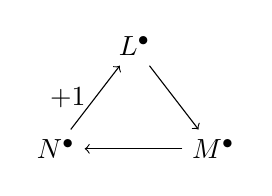
\begin{tikzpicture}[baseline=(current bounding box.center)]
    \node (L) at (1,1.3)
    {$L^\bullet$}; \node (N) at (0,0)
    {$N^\bullet$}; \node (M) at (2,0)
    {$M^\bullet$}; \draw[->] (L) -- (M); \draw[->] (M) -- (N);
    \draw[->] (N) -- (L) node[midway, left] {$+1$};
  \end{tikzpicture}
\]
which we understand to be exact at its three vertices: this is an
\emph{exact triangle} in $\categ{C}(\categ{A})$. The arrow marked by
$+1$ is in this case simply the zero-morphism; the $+1$ records the
fact that we are going to view this as a morphism from $N$ to the
shift $L[1]^\bullet$ of $L^\bullet$ (after all, $0$ is $0$ in all
degrees). Thus, the triangle is shorthand for the impressive
commutative 3D-diagram
% TODO: diagram of the "impressive commutative 3D-diagram" -- a
% stacked lattice showing, for each degree i-1, i, i+1, the triangle
% N^i <-- M^i, with a diagonal 0-arrow N^i -> L^i and vertical arrows
% L^i -> L^{i+1}, M^i -> M^{i+1}, N^i -> N^{i+1} connecting successive
% layers (page 601)
or (understanding the morphisms in the complexes) the single long
sequence
\[
  \dots \longrightarrow N^{i-1} \xrightarrow{0} L^i \longrightarrow
  M^i \longrightarrow N^i \xrightarrow{0} L^{i+1} \longrightarrow
  \dots,
\]
whose exactness is equivalent to the exactness of the original short
exact sequence of complexes. In \S{}3.3 we have obtained from this
\emph{another} long exact sequence,
\[
  \dots \longrightarrow H^{i-1}(N^\bullet) \xrightarrow{\delta^{i-1}}
  H^i(L^\bullet) \longrightarrow H^i(M^\bullet) \longrightarrow
  H^i(N^\bullet) \xrightarrow{\delta^i} H^{i+1}(L^\bullet)
  \longrightarrow \dots,
\]
which we fold again into an exact triangle:
\[
  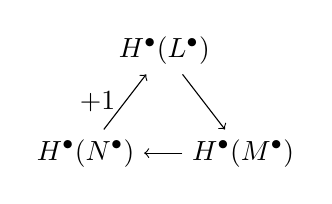
\begin{tikzpicture}[baseline=(current bounding box.center)]
    \node (L) at (1,1.3)
    {$H^\bullet(L^\bullet)$}; \node (N) at (0,0)
    {$H^\bullet(N^\bullet)$}; \node (M) at (2,0)
    {$H^\bullet(M^\bullet)$}; \draw[->] (L) -- (M); \draw[->] (M) --
    (N); \draw[->] (N) -- (L) node[midway, left] {$+1$};
  \end{tikzpicture}
\]
This time the morphism marked $+1$ is the interesting connecting
morphism (while the morphisms in the cohomology complexes are zero;
see the end of \S{}3.2).

Thus, the `long exact cohomology sequence' takes us from a certain
exact triangle to another exact triangle. The first triangle arises
from a short exact sequence of complexes (the `connecting morphism' is
$0$), while the second does not (the connecting morphism is in general
nonzero).

Clearly something interesting is going on. Triangles obtained from
short exact sequences of complexes in $\categ{C}(\categ{A})$ appear to
be `special' and give rise to other exact triangles through
cohomology.

Actually, the situation may make the reader somewhat uncomfortable.
While two sides of the cohomology triangle are obtained by simply
applying the cohomology functor to the corresponding sides of the
original triangle, the third one is obtained by a different process,
involving the connecting morphism. The reader may feel that there
should be a mechanism to go from a triangle defined in terms of an
exact sequence to its counterpart in cohomology by simply applying the
cohomology functor.

This is indeed so. There is an important notion of `distinguished'
triangle, in a category $\categ{K}(\categ{A})$ closely associated with
$\categ{C}(\categ{A})$ and that we will encounter
later\footnote{Beware that some authors call the distinguished
  triangles `exact'; there is some room for confusion, since the
  special exact triangles in the present discussion are not `exact'
  from this viewpoint.} (\S{}5). As with the `special' triangles given
above, distinguished triangles lead to long exact sequences in
cohomology, and in a somewhat more direct fashion. Distinguished
triangles satisfy a number of axioms, which define
$\categ{K}(\categ{A})$ as a \emph{triangulated category}. Exploring
these concepts at any level of depth is well beyond the scope of this
book, but towards the end of the chapter I will try to clarify these
last cryptic remarks (\S{}9.2).

\subsection*{Exercises}

\begin{exer}{\exerused{}}{exer:homol:3.1}
  Let $(M^\bullet, d^\bullet)$ be a resolution of an object $A$ of an
  abelian category. Verify that there are exact complexes
  \[
    \dots \xrightarrow{d^{-3}} M^{-2} \xrightarrow{d^{-2}} M^{-1}
    \longrightarrow \ker d^0 \longrightarrow A \longrightarrow 0
    \longrightarrow \dots,
  \]
  \[
    \dots \longrightarrow 0 \longrightarrow A \longrightarrow
    \cokerd^{-1} \longrightarrow M^1 \xrightarrow{d^1}
    M^2 \xrightarrow{d^2} \dots
  \]
  and that replacing $A$ by $0$ in these complexes produces new
  resolutions of $A$. [\S{}\ref{subsec:homol:reminder-of-basic-definitions-general-strategy}, \S{}\ref{subsec:homol:recovering-a}]
\end{exer}
\begin{exer}{$\lnot$}{exer:homol:3.2}
  Let $\categ{I}$ be the category whose objects are the integers and
  where $\Hom_{\categ{I}}(m, n)$ consists of a singleton if $m \leq n$
  and is $\emptyset$ otherwise (cf.\ \Cref{exam:prelims:set-is-a-category}). Show that the
  category $\categ{C}(\categ{A})$ of cochain complexes is a full
  subcategory of the abelian category $\categ{A}^{\categ{I}}$. [\ref{exer:homol:3.3}]
\end{exer}
\begin{exer}{\exerused{}}{exer:homol:3.3}
  Verify that the category $\categ{C}(\categ{A})$ of cochain complexes
  in an abelian category, defined in \S{}3.2, is itself an abelian
  category. (You can do this either `by hand' or by applying
  Exercises~3.2 and~2.14.) [\S{}\ref{subsec:homol:the-category-of-complexes}]
\end{exer}
\begin{exer}{$\lnot$}{exer:homol:3.4}
  Let $\categ{A}$ be an abelian category. Define a category
  $\operatorname{Seq}(\categ{A})$ whose objects are short exact
  sequences in $\categ{A}$ and where morphisms are commutative
  diagrams
  \[\begin{tikzcd}[column sep=small]
      0 \arrow[r] & A_1 \arrow[r] \arrow[d] & B_1 \arrow[r] \arrow[d]
      &
      C_1 \arrow[r] \arrow[d] & 0 \\
      0 \arrow[r] & A_2 \arrow[r] & B_2 \arrow[r] & C_2 \arrow[r] & 0
    \end{tikzcd}\] Thus, $\operatorname{Seq}(\categ{A})$ may be viewed
  as a full subcategory of $\categ{C}(\categ{A})$.
  \begin{itemize}
  \item Prove that $\operatorname{Seq}(\categ{A})$ is an additive
    category.
  \item Prove that $\operatorname{Seq}(\categ{A})$ has kernels and
    cokernels. (Watch out: these are not the same as in
    $\categ{C}(\categ{A})$. Keep the snake lemma in mind.)
  \item Show that, for every object $X$ of $\categ{A}$,
    \[\begin{tikzcd}[column sep=small]
        0 \arrow[r] & 0 \arrow[r] & X \arrow[r, "\id_X"]
        \arrow[d, "\id_X"'] &
        X \arrow[r] & 0 \\
        0 \arrow[r] & X \arrow[r, "\id_X"'] & X
        \arrow[r] & 0 \arrow[r] & 0 \arrow[from=1-4, to=2-2,
        "\id_X"']
      \end{tikzcd}\] is both a monomorphism and an epimorphism in
    $\operatorname{Seq}(\categ{A})$, although it is neither a
    monomorphism nor an epimorphism in $\categ{C}(\categ{A})$ if
    $X \neq 0$.
  \item Prove that $\operatorname{Seq}(\categ{A})$ is not abelian if
    $\categ{A}$ has nonzero objects.
  \end{itemize} [\S{}\ref{subsec:homol:abelian-categories}, \ref{exer:homol:3.11}]
\end{exer}
\begin{exer}{\exerused{}}{exer:homol:3.5}
  Let $(L^\bullet, d^\bullet_{L^\bullet})$ be a cochain complex;
  define new differentials $d'^\bullet_{L^\bullet}$ by arbitrarily
  changing the sign of $d^i_{L^\bullet}$:
  $d'^i_{L^\bullet} = \pm d^i_{L^\bullet}$. Show that
  $(L^\bullet, d'^\bullet_{L^\bullet})$ is a cochain complex
  isomorphic to $(L^\bullet, d^\bullet_{L^\bullet})$. [\S{}\ref{subsec:homol:the-category-of-complexes}]
\end{exer}
\begin{exer}{}{exer:homol:3.6}
  Provide an arrow-theoretic proof of \Cref{homol:3.4} (cf.\ \Cref{homol:3.1}).
\end{exer}
\begin{exer}{}{exer:homol:3.7}
  Let $\categ{A}$, $\categ{B}$ be abelian categories. An additive
  functor $\mathscr{F} : \categ{A} \to \categ{B}$ is \emph{exact} if
  it maps short exact sequences in $\categ{A}$ to short exact
  sequences in $\categ{B}$. Prove that exact functors commute with
  cohomology: if $\mathscr{F}$ is exact and $L^\bullet$ is a cochain
  complex in $\categ{A}$, then
  $H^\bullet(\mathscr{F}(L^\bullet)) \cong
  \mathscr{F}(H^\bullet(L^\bullet))$, where $\mathscr{F}(L^\bullet)$
  denotes the cochain complex in $\categ{B}$ obtained by applying
  $\mathscr{F}$ to all objects and morphisms in $L^\bullet$.

  In particular, the image of an exact complex through an exact
  functor is still an exact complex (cf.\ \Cref{linrep:exer:1.23}).
\end{exer}
\begin{exer}{\exerused{}}{exer:homol:3.8}
  For any $i$, give an example of a short exact sequence of complexes
  \[
    0 \longrightarrow L^\bullet \longrightarrow M^\bullet
    \longrightarrow N^\bullet \longrightarrow 0
  \]
  such that the sequence
  \[
    0 \longrightarrow H^i(L^\bullet) \longrightarrow H^i(M^\bullet)
    \longrightarrow H^i(N^\bullet) \longrightarrow 0
  \]
  is not exact at either $H^i(L^\bullet)$ or $H^i(N^\bullet)$.
  [\S{}\ref{subsec:homol:universal-property-of-the-derived-functor}]
\end{exer}
\begin{exer}{\exerused{}}{exer:homol:3.9}
  Provide the gory details for the long exact cohomology sequence
  (\Cref{homol:3.5}). [\S{}\ref{subsec:homol:the-long-exact-cohomology-sequence}, \ref{exer:homol:3.10}]
\end{exer}
\begin{exer}{\exerused{}}{exer:homol:3.10}
  Here is a way to reduce \Cref{exer:homol:3.9} to the snake lemma itself.

  Every complex $(L^\bullet, \lambda^\bullet)$ determines a complex
  $\ker^\bullet$, with the object\footnote{Of course $\ker$ and
    $\coker$ mean the target and source of the arrows
    $\ker$ and $\coker$, respectively.}
  $\ker\lambda^{i+1}$ in degree $i$, connected by zero-morphisms, and
  a complex $\coker^\bullet$, with the object
  $\coker\lambda^{i-1}$ in degree $i$, also connected by
  zero-morphisms.

  Prove that $\lambda^\bullet$ induces a morphism
  $\overline{\lambda}^\bullet : \coker^\bullet \to
  \ker^\bullet$ in the abelian category of complexes, such that
  $\ker\overline{\lambda}^\bullet \cong H^\bullet(L^\bullet)$ and
  $\coker\overline{\lambda}^\bullet \cong
  H(L^\bullet)[1]^\bullet$.

  Now work out the whole long exact cohomology sequence as a
  consequence of the snake lemma. (You will use the version of the
  snake lemma given in \Cref{rem:rings:snake-lemma-relaxed-hypotheses}.) [\S{}\ref{subsec:homol:the-long-exact-cohomology-sequence}, \ref{exer:homol:3.13}]
\end{exer}
\begin{exer}{$\lnot$}{exer:homol:3.11}
  Prove that the long exact cohomology sequence is functorial, in the
  sense that it defines a covariant functor from the category
  $\operatorname{Seq}(\categ{C}(\categ{A}))$ of short exact sequences
  (cf.\ \Cref{exer:homol:3.4}) of complexes to the category of
  complexes. [\ref{exer:homol:7.13}]
\end{exer}
\begin{exer}{}{exer:homol:3.12}
  Redo \Cref{exer:rings:7.17}.
\end{exer}
\begin{exer}{}{exer:homol:3.13}
  The viewpoint in \Cref{exer:homol:3.10} admits the following straightforward
  generalization.

  Let $\categ{A}$ be an abelian category. Define a new category
  $d\categ{A}$, whose objects are pairs $(A, d)$, where $A$ is an
  object of $\categ{A}$ and $d : A \to A$ is a morphism (the
  `differential') such that $d^2 = 0$. Morphisms
  $(A, d_A) \to (B, d_B)$ in $d\categ{A}$ are morphisms
  $\varphi : A \to B$ commuting with the differentials:
  $d_B\varphi = \varphi d_A$.
  \begin{itemize}
  \item Prove that $d\categ{A}$ is an abelian category.
  \item For any $(A, d)$ in $d\categ{A}$, prove that $d$ induces a
    morphism $\bar d : \cokerd \to \ker d$.
  \item Define $H(A, d)$ to be $\ker \bar d$. Prove that
    $\coker\bar d \cong H(A, d)$.
  \item Show that $H$ defines an additive functor
    $d\categ{A} \to \categ{A}$ and that this functor is not exact in
    general.
  \item However, prove that every short exact sequence
    \[
      0 \longrightarrow (A, d_A) \longrightarrow (B, d_B)
      \longrightarrow (C, d_C) \longrightarrow 0
    \]
    in $d\categ{A}$ induces an exact triangle (in the sense of
    \S{}3.4)
    \[
      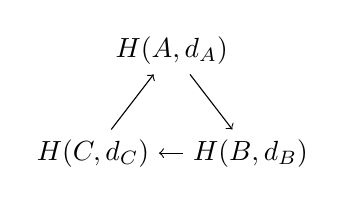
\begin{tikzpicture}[baseline=(current bounding box.center)]
        \node (A) at (1,1.3)
        {$H(A,d_A)$}; \node (C) at (0,0)
        {$H(C,d_C)$}; \node (B) at (2,0)
        {$H(B,d_B)$}; \draw[->] (A) -- (B); \draw[->] (B) -- (C);
        \draw[->] (C) -- (A);
      \end{tikzpicture}
    \]
  \end{itemize}
\end{exer}
\begin{exer}{\exerused{}}{exer:homol:3.14}
  Prove that if one of the vertices of a `special' triangle arising
  from a short exact sequence of complexes (as in \S{}3.4) is exact,
  then the other two vertices have isomorphic cohomologies, possibly
  up to a shift. [\S{}\ref{subsec:homol:the-mapping-cone-of-a-morphism}]
\end{exer}
\begin{exer}{$\lnot$}{exer:homol:3.15}
  Define a `Grothendieck group' and a `universal Euler characteristic'
  $\chi$ for any abelian category $\categ{A}$, in the style of the
  construction given in \ref{subsec:linalg:euler-characteristic-and-the-grothendieck-group}.

  Extend $\chi$ to all bounded cochain complexes $M^\bullet$ in
  $\categ{A}$, by setting
  $\chi(M^\bullet) := \sum_i (-1)^i \chi(M^i)$. Prove that
  $\chi(M^\bullet) = \chi(H^\bullet(M^\bullet))$. For every short
  exact sequence of bounded complexes
  $0 \to L^\bullet \to M^\bullet \to N^\bullet \to 0$, prove that
  $\chi(M^\bullet) = \chi(L^\bullet) + \chi(N^\bullet)$. [\ref{exer:homol:4.3}, \ref{exer:homol:9.1}]
\end{exer}

\section{Cones and homotopies}
\label{sec:homol:cones-and-homotopies}

If $\alpha^\bullet : L^\bullet \to M^\bullet$ is a morphism of cochain
complexes, it is natural to try to describe the morphism induced in
cohomology:
\[
  H^\bullet(\alpha^\bullet) : H^\bullet(L^\bullet) \to
  H^\bullet(M^\bullet).
\]
However, I have pointed out that $H^\bullet$ is not an exact functor,
and this seems to pose an obstacle to simple-minded strategies aimed
at describing (for example) the kernel or cokernel of
$H^\bullet(\alpha^\bullet)$ in terms of the kernel or cokernel of
$\alpha^\bullet$. The long exact cohomology sequence may be used to
compensate for this lack of exactness; we will see how in \S{}4.1. We
will also begin exploring a very important condition (`homotopy')
guaranteeing that two given morphisms of complexes induce the same
morphism in cohomology. Homotopies will be so important that they will
lead us later on to change our notion of morphisms between complexes
and construct a new `homotopic category' of complexes (see \S{}5).

\subsection{The mapping cone of a morphism}
\label{subsec:homol:the-mapping-cone-of-a-morphism}

Let $\alpha^\bullet : L^\bullet \to M^\bullet$ be a morphism of
cochain complexes. The \emph{mapping cone} $MC(\alpha)^\bullet$ of
$\alpha^\bullet$ will allow us to recover $H^\bullet(\alpha^\bullet)$
as the connecting morphism in a long exact cohomology sequence, as
constructed in \S{}3.3. In fact, the mapping cone will give us the
third vertex of a `special' triangle (cf.\ the end of \S{}3.4):
\[
  (\dagger) \quad
  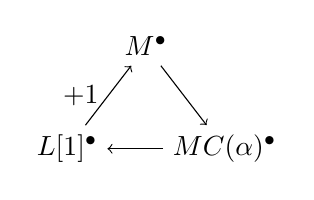
\begin{tikzpicture}[baseline=(current bounding box.center)]
    \node (M) at (1,1.3)
    {$M^\bullet$}; \node (L) at (0,0)
    {$L[1]^\bullet$}; \node (C) at (2,0)
    {$MC(\alpha)^\bullet$}; \draw[->] (M) -- (C); \draw[->] (C) --
    (L); \draw[->] (L) -- (M) node[midway, left] {$+1$};
  \end{tikzpicture}
\]
The degree-increasing morphism is the zero-morphism here (as in the
`special' triangles encountered in \S{}3.4); but taking cohomology
\[
  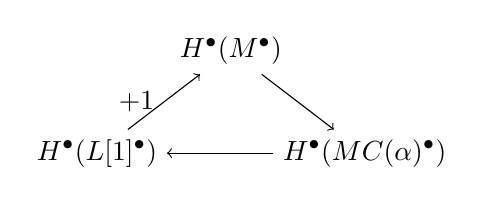
\begin{tikzpicture}[baseline=(current bounding box.center)]
    \node (M) at (1.7,1.3)
    {$H^\bullet(M^\bullet)$}; \node (L) at (0,0)
    {$H^\bullet(L[1]^\bullet)$}; \node (C) at (3.4,0)
    {$H^\bullet(MC(\alpha)^\bullet)$}; \draw[->] (M) -- (C); \draw[->]
    (C) -- (L); \draw[->] (L) -- (M) node[midway, left] {$+1$};
  \end{tikzpicture}
\]
we will obtain morphisms
\[
  H^{i+1}(L^\bullet) = H^i(L[1]^\bullet) \longrightarrow
  H^{i+1}(M^\bullet)
\]
that, I claim, will be nothing but the morphisms induced in cohomology
by the given morphism $\alpha^\bullet$. Thus, the morphisms induced in
cohomology cannot be extended to exact sequences (that would clearly
be asking too much), but they can be extended to triangles arising by
applying cohomology to an appropriate exact sequence of complexes.

Incidentally, the triangle $(\dagger)$ displayed above (but with the
degree-increasing morphism replaced by $-\alpha^\bullet$) will be the
prototype of the `distinguished triangles' mentioned in \S{}3.4 (cf.\
\S{}9.2).

\emph{Construction of the mapping cone.} The objects of
$MC(\alpha)^\bullet$ are simply direct sums of objects of $L^\bullet$
and $M^\bullet$:
\[
  MC(\alpha)^i := L[1]^i \oplus M^i = L^{i+1} \oplus M^i;
\]
but the morphisms
$d^i_{MC(\alpha)^\bullet} : MC(\alpha)^i \to MC(\alpha)^{i+1}$ are not
the `obvious' ones, but rather
\[
  d^i_{MC(\alpha)^\bullet}(\ell, m) := (-d^{i+1}_{L^\bullet}(\ell),
  \alpha^{i+1}(\ell) + d^i_{M^\bullet}(m)).
\]
The sign in the first component is inherited from the shifting of
$L^\bullet$; thus, the first component is simply the differential of
$L[1]^\bullet$. The second component mixes $\alpha^\bullet$ (or rather
its shift $\alpha[1]^\bullet$) and the differential of
$M^\bullet$. The reader should verify that
$d^{i+1}_{MC(\alpha)^\bullet} \circ d^i_{MC(\alpha)^\bullet} = 0$, so
that $MC(\alpha)^\bullet$ is indeed a cochain complex (\Cref{exer:homol:4.1});
this is where the sign comes in. The mapping cone is a special case of
the `total complex' determined by a double complex, to be explored
later (\S{}8.2).

Pictorially, $MC(\alpha)^\bullet$ looks like this:
\[\begin{tikzcd}[column sep=large, row sep=small]
    \dots \arrow[r] & L^{i+1} \arrow[r, "-d^{i+1}_{L^\bullet}"] &
    L^{i+2} \arrow[r] & \dots \\
    & \oplus & \oplus & \\
    \dots \arrow[r] & M^i \arrow[r, "d^i_{M^\bullet}"'] & M^{i+1}
    \arrow[r] & \dots \arrow[from=1-2, to=3-3, "\alpha^{i+1}"
    description]
  \end{tikzcd}\] There are evident morphisms of complexes
$M^\bullet \to MC(\alpha)^\bullet$ and
$MC(\alpha)^\bullet \to L[1]^\bullet$, induced by the natural
morphisms
$M^i \longrightarrow L^{i+1} \oplus M^i \longrightarrow
L^{i+1}$. Since the sequences
\[
  0 \longrightarrow M^i \longrightarrow L[1]^i \oplus M^i
  \longrightarrow L[1]^i \longrightarrow 0
\]
are all exact, the sequence of complexes
\[
  0 \longrightarrow M^\bullet \longrightarrow MC(\alpha)^\bullet
  \longrightarrow L[1]^\bullet \longrightarrow 0
\]
is exact.
\begin{prop}{}{homol:4.1}
  There is an exact triangle
  \[
    \begin{tikzpicture}[baseline=(current bounding box.center)]
      \node (M) at (1.7,1.3)
      {$H^\bullet(M^\bullet)$}; \node (L) at (0,0)
      {$H^\bullet(L[1]^\bullet)$}; \node (C) at (3.4,0)
      {$H^\bullet(MC(\alpha)^\bullet)$}; \draw[->] (M) -- (C);
      \draw[->] (C) -- (L); \draw[->] (L) -- (M) node[midway, left]
      {$\substack{+1 \\ \delta}$};
    \end{tikzpicture}
  \]
  where the connecting morphism $\delta$ is the morphism induced by
  $\alpha^\bullet$ in cohomology.
\end{prop}

\begin{proof}
  The existence of the triangle is a direct consequence of
  \Cref{homol:3.5}; all we have to check is that the connecting morphism
  indeed agrees with the morphism induced by $\alpha^\bullet$.
  Chasing the diagram
  \[\begin{tikzcd}[column sep=small]
      & \vdots & \vdots & \vdots & \\
      0 \arrow[r] & M^i \arrow[r] \arrow[u] &
      L^{i+1} \oplus M^i \arrow[r] \arrow[u] & L^{i+1} \arrow[r] \arrow[u] & 0 \\
      0 \arrow[r] & M^{i-1} \arrow[r] \arrow[u] &
      L^i \oplus M^{i-1} \arrow[r] \arrow[u] & L^i \arrow[r] \arrow[u] & 0 \\
      & \vdots \arrow[u] & \vdots \arrow[u] & \vdots \arrow[u] &
    \end{tikzcd}\] with a class in
  $H^{i-1}(L[1]^\bullet) = H^i(L^\bullet)$ represented by
  $\ell \in L^i$ (such that $d^i_{L^\bullet}(\ell) = 0$), we find that
  $\alpha^i(\ell)$, viewed as an element of $MC(\alpha)^i$ via
  $(0, \alpha^i(\ell))$, is cohomologous to $(\ell, 0)$,
  % TODO: diagram chase verifying (0, alpha^i(ell)) and (ell, 0)
  % represent the same class in MC(alpha)^i (page 607)
  which maps to $\ell$ under $MC(\alpha)^\bullet \to L[1]^\bullet$;
  this verifies the claim.
\end{proof}

\begin{coro}{}{homol:4.2}
  Let $\alpha^\bullet : L^\bullet \to M^\bullet$ be a morphism of
  cochain complexes. Then the induced morphism
  $H^\bullet(L^\bullet) \to H^\bullet(M^\bullet)$ is an isomorphism if
  and only if the mapping cone $MC(\alpha)^\bullet$ is an exact
  complex.

  (Cf.\ \Cref{exer:homol:3.14}.)
\end{coro}

I should mention that mapping cones arose in topology: the mapping
cone of a continuous map $f : X \to Y$ is obtained by considering
$X \times [0,1]$, identifying $X \times 0$ to a point, and stitching
$X \times 1$ to $Y$ by means of $f$. Analyzing chains of this space
leads to the (homological version of the) `algebraic' mapping cone
considered above.

\subsection{Quasi-isomorphisms and derived categories}
\label{subsec:homol:quasi-isomorphisms-and-derived-categories}

A component of our main strategy consists of understanding when
cochain complexes `have a good reason' to have the same cohomology.
\Cref{homol:4.2} provides us with such a reason. The morphisms singled
out in that statement have a name:

\begin{defn}{}{homol:4.3}
  A morphism $\alpha^\bullet$ of cochain complexes is a
  \emph{quasi-isomorphism} if it induces an isomorphism in cohomology.
\end{defn}

By \Cref{homol:4.2}, this condition is equivalent to the exactness of the
mapping cone of $\alpha^\bullet$.

\begin{exam}{}{homol:4.4}
  The datum of a resolution $M^\bullet$ of an object $A$ of an abelian
  category $\categ{A}$, as in \Cref{homol:3.2} and with $M^i = 0$ for
  $i > 0$, is the same as the datum of a quasi-isomorphism
  \[
    M^\bullet \xrightarrow{\text{q-iso.}} \iota(A)
  \]
  where $\iota$ places $A$ in degree $0$ and $0$ in all other
  degrees. Here is a larger version of the same diagram:
  \[\begin{tikzcd}[column sep=small]
      \dots \arrow[r] & M^{-2} \arrow[r, "d^{-2}_{M^\bullet}"]
      \arrow[d] & M^{-1} \arrow[r, "d^{-1}_{M^\bullet}"] \arrow[d] &
      M^0 \arrow[r, "d^0_{M^\bullet}"] \arrow[d] & 0 \arrow[r] \arrow[d] & \dots \\
      \dots \arrow[r] & 0 \arrow[r] & 0 \arrow[r] & A \arrow[r] & 0
      \arrow[r] & \dots
    \end{tikzcd}\] where the only nontrivial vertical map is the
  cokernel of $d^{-1}_{M^\bullet}$.
\end{exam}

Thus, quasi-isomorphisms may be viewed as generalizations of more
simple-minded resolutions. Also note that the mapping cone of a
resolution as in \Cref{homol:4.4} is obtained (as the reader should check)
by shifting the complex `one step to the left' and completing it with
$A$, obtaining the \emph{exact} complex:
\[
  \dots \longrightarrow M^{-1} \xrightarrow{-d^{-1}_{M^\bullet}} M^0
  \xrightarrow{\cokerd^{-1}_{M^\bullet}} A
  \longrightarrow 0 \longrightarrow \dots.
\]
This is nothing but our other point of view on resolutions (as in
\ref{subsec:linalg:finitely-presented-modules-and-free-resolutions}).

\begin{rem}{}{homol:4.5}
  Quasi-isomorphisms with fixed target (resp., source) form a category
  in a natural way, which I will leave to the reader to make
  precise. In particular, resolutions in
  $\categ{C}^{\leq 0}(\categ{A})$ (resp.,
  $\categ{C}^{\geq 0}(\categ{A})$) of a given object of $\categ{A}$,
  as in \Cref{homol:4.4}, form a category.
\end{rem}

Wouldn't it be nice if quasi-isomorphisms were actual isomorphisms,
that is, if they were invertible? In general, they are not. The
following example will arise several times to ward off any such hopes.

\begin{exam}{}{homol:4.6}
  In $\categ{C}(\categ{Ab})$, the morphism of complexes
  \[\begin{tikzcd}[column sep=small]
      \dots \arrow[r] & 0 \arrow[r] \arrow[d] & \Z \arrow[r, "\cdot
      2"] \arrow[d] &
      \Z \arrow[r] \arrow[d, "\pi"] & 0 \arrow[r] \arrow[d] & \dots \\
      \dots \arrow[r] & 0 \arrow[r] & 0 \arrow[r] & \dfrac{\Z}{2\Z}
      \arrow[r] & 0 \arrow[r] & \dots
    \end{tikzcd}\] where $\pi$ is the natural projection, is a
  quasi-isomorphism, but it does not have an inverse since there are
  no nontrivial homomorphisms $\Z/2\Z \to \Z$.
\end{exam}

In fact, this example shows that `quasi-isomorphism' is not even an
equivalence relation (it is not symmetric). This is too bad---if it
were, then the `equivalence class of a complex' would be the most
natural candidate for the entity carrying the maximal amount of
cohomological information of a complex.

I will stop short of defining a `quasi-isomorphism relation': in this
book, quasi-isomorphism is simply a particular quality of a morphism
of cochain complexes, not a relation. In any case recall that, even in
the context of sets, taking the quotient by an equivalence relation is
not the `primary' object of interest: the quotient is just the
solution to the natural universal problem of studying functions to
other sets with identical behavior on `equivalent'
elements. \emph{This} is the primary objective.

Similarly, the primary objective in the present context is not so much
to identify together all complexes linked by a quasi-isomorphism, as
it is to be able to shuttle information back and forth between such
complexes. The natural way to accomplish this is to study environments
in which quasi-isomorphisms do have inverses. More precisely, it
consists of studying additive functors
\[
  \mathscr{F} : \categ{C}(\categ{A}) \longrightarrow \categ{D}
\]
such that $\mathscr{F}(\rho^\bullet)$ is an isomorphism for every
quasi-isomorphism $\rho^\bullet$. (Cohomology is such a functor.)

This sounds like yet another universal problem, and the natural line
of attack would be to solve it as such, that is, to define (if
possible) a category $\categ{D}(\categ{A})$ endowed with an additive
functor $\categ{C}(\categ{A}) \to \categ{D}(\categ{A})$ such that
quasi-isomorphisms in $\categ{C}(\categ{A})$ are mapped to
isomorphisms in $\categ{D}(\categ{A})$ and through which every
$\mathscr{F}$ as above must factor uniquely:
\[\begin{tikzcd}
    \categ{C}(\categ{A}) \arrow[r, "\mathscr{F}"] \arrow[d] & \categ{D} \\
    \categ{D}(\categ{A}) \arrow[ur, dashed, "\exists!"']
  \end{tikzcd}\] To be honest, we should take such a statement with a
grain of salt: the natural environment in which we should pose this
universal problem would be a `category of categories', and we have not
defined such a thing in this book. A category $\categ{D}(\categ{A})$
as above \emph{does} exist, at least if a certain `localization'
process can be carried out\footnote{There may be set-theoretic issues
  with this process. However, these play no role in the cases we will
  consider, in which $\categ{A}$ has `enough projectives' or `enough
  injectives'.}: it is the \emph{derived category} of $\categ{A}$.
`Bounded' versions $\categ{D}^-(\categ{A})$, $\categ{D}^+(\categ{A})$,
and more, are solutions to the corresponding universal problems for
appropriately bounded complexes.

These derived categories answer the main question underlying our
strategy, of understanding `what' in a complex really determines its
cohomology: the answer amounts to viewing the complex in the
appropriate derived category. The construction of
$\categ{D}(\categ{A})$ consists roughly of taking the same objects as
$\categ{C}(\categ{A})$ and formally inverting the
quasi-isomorphisms. The details of this construction are somewhat
involved and are best left to more advanced texts. But we will be able
to capture its essence in this book, at least in lucky cases (when the
abelian category has `enough injectives' or `enough projectives'; see
\Cref{defn:homol:5.7}).

The derived category has the unfortunate reputation of being an overly
abstract notion, and there are fundamental questions about whether it
really is the best approach to an abstract study of cohomology. This
is partly because the derived category of an abelian category is
\emph{not} an abelian category and simple notions such as kernel,
cokernel, exact sequences are not available in
$\categ{D}(\categ{A})$. This adds a substantial layer of complication
to the theory.

On the other hand, going past these difficulties, one finds that
enough structure remains to do much homological algebra: objects in
$\categ{D}(\categ{A})$ have cohomology, and there are `distinguished
triangles' (cf.\ \S{}3.4) abstracting exact sequences and giving long
exact cohomology sequences. The derived category is a
\emph{triangulated category}, like the more manageable homotopic
category $\categ{K}(\categ{A})$ that we will soon define. Its uses go
beyond the confines of algebra or even mathematics: an approach to the
understanding of `D-branes' in string theory is based on derived
categories.

To get a sense of how counterintuitive $\categ{D}(\categ{A})$ must be,
note that the zero-morphism $0 : M^\bullet \to M^\bullet$ may well be
a quasi-isomorphism: in fact, this is so precisely when $M^\bullet$ is
exact. Well, in any category $\categ{D}$ as above (and in particular
in the derived category $\categ{D}(\categ{A})$) this zero-morphism
remains the zero-morphism, \emph{but} it comes equipped with an
inverse when it is a quasi-isomorphism. Thus, in the derived category
the zero-morphism on a complex involving nonzero objects may well be
invertible! This says that complexes that are nonzero in
$\categ{C}(\categ{A})$ may become zero-objects in the derived
category.

\begin{lem}{}{homol:4.7}
  Let $\categ{D}$ be an additive category, and let
  $\mathscr{F} : \categ{C}(\categ{A}) \to \categ{D}$ be an additive
  functor such that $\mathscr{F}(\rho^\bullet)$ is an isomorphism for
  every quasi-isomorphism $\rho^\bullet$.
  \begin{itemize}
  \item Let $M^\bullet$ be an exact complex in $\categ{C}(\categ{A})$.
    Then the complex $\mathscr{F}(M^\bullet)$, obtained by applying
    $\mathscr{F}$ to the objects and morphisms of $M^\bullet$, is a
    zero-object in $\categ{D}$.
  \item Let $\alpha^\bullet : L^\bullet \to N^\bullet$ be a morphism
    in $\categ{C}(\categ{A})$ that factors through an exact complex,
    \[\begin{tikzcd}
        L^\bullet \arrow[rr, "\alpha^\bullet"] \arrow[dr] & & N^\bullet \\
        & M^\bullet \arrow[ur]
      \end{tikzcd}\] with $M^\bullet$ exact. Then
    $\mathscr{F}(\alpha^\bullet)$ is the zero-morphism.
  \end{itemize}
\end{lem}

\begin{proof}
  The second claim follows from the first, since by applying
  $\mathscr{F}$ to the given diagram we obtain
  \[\begin{tikzcd}
      \mathscr{F}(L^\bullet) \arrow[rr, "\mathscr{F}(\alpha^\bullet)"]
      \arrow[dr] & & \mathscr{F}(N^\bullet) \\
      & \mathscr{F}(M^\bullet) \arrow[ur]
    \end{tikzcd}\] and we see that $\mathscr{F}(\alpha^\bullet)$
  factors through a zero-object of $\categ{D}$.

  To verify the first claim, note that since $M^\bullet$ is exact, the
  zero-morphism $M^\bullet \to M^\bullet$ is a quasi-isomorphism;
  hence it is mapped to an invertible morphism by $\mathscr{F}$:
  \[
    \underbrace{\mathscr{F}(M^\bullet) \xrightarrow{\mathscr{F}(0)}
      \mathscr{F}(M^\bullet) \xrightarrow{\mathscr{F}(0)^{-1}}
      \mathscr{F}(M^\bullet)}_{\id_{\mathscr{F}(M^\bullet)}}
  \]
  Since $\mathscr{F}$ is additive, $\mathscr{F}(0) = 0$. It follows
  that $\id_{\mathscr{F}(M^\bullet)} = 0$ and hence that
  $\mathscr{F}(M^\bullet)$ is a zero-object of $\categ{D}$, by
  \Cref{exer:homol:1.6}.
\end{proof}

In the next several sections I will chase the notion of derived
category, aiming to understand it rather concretely in particularly
favorable circumstances. \emph{We will take it for granted that these
  categories exist.} A detailed definition of these objects, or a
treatment of triangulated categories, is beyond the scope of this
book.

\subsection{Homotopy}
\label{subsec:homol:homotopy}

The foregoing considerations put our strategy into focus: we are after
constructions that determine cochain complexes `up to
quasi-isomorphism'. However, quasi-isomorphisms appear hard to deal
with directly. Thus, we look for more manageable notions that may work
as an effective replacement.

Like the mapping cone, this line of approach also owes its origins to
topology: in topology, `homeomorphism' is often too harsh a
requirement, while `homotopy equivalence' is a more malleable but
still adequate notion. For example, homotopy equivalent topological
spaces have the same homology. Distilling the algebra out of this
notion leads to an analog at the level of complexes.

To see how this is done, recall that if $f$, $g$ are \emph{homotopic}
continuous functions between two topological spaces $X$ and $Y$, then
$f$ and $g$ induce the same map on the homology of the spaces.  To
remind yourself of how this works, look at the picture:
% TODO: diagram of a homotopy h(a) between f(a) and g(a): a
% curved/wavy region bounded by f(a) on the left, g(a) on the right,
% delta_+ on top and delta_- on bottom, with h(a) labeling the
% interior surface (page 611)
This is supposed to represent the action of a homotopy between $f$ and
$g$ on a chain $a$ in $X$: $h(a)$ is obtained by mapping
$a \times [0,1]$ to $Y$ so as to get $f(a)$ when restricting to
$a \times \{0\}$ and to get $g(a)$ when restricting to
$a \times \{1\}$. Note that $h(a)$ is a chain of dimension $1$ higher
than the dimension of $a$, and that the boundary $\partial h(a)$ of
this chain consists of $f(a)$, $g(a)$ and of the restriction of $h$ to
the boundary $\partial a$ of $a$: taking the boundary
`counterclockwise',
\[
  \partial h(a) = g(a) - \delta_+ - f(a) + \delta_- = g(a) - f(a) -
  h(\partial a)
\]
(or so it would seem from the picture! As presented here, this is of
course at best a plausibility argument; it can be made rigorous, but
that is someone else's business). That is,
\[
  g(a) - f(a) = \partial h(a) + h(\partial a).
\]
Since boundaries vanish in homology, $f(a)$ and $g(a)$ will agree in
homology.

Here is the translation into algebra of this pleasant geometric
situation:

\begin{defn}{}{homol:4.8}
  A \emph{homotopy} $h$ between two morphisms of cochain complexes
  $\alpha^\bullet, \beta^\bullet : L^\bullet \to M^\bullet$ is a
  collection of morphisms
  \[
    h^i : L^i \to M^{i-1}
  \]
  such that $\forall i$
  \[
    \beta^i - \alpha^i = d^{i-1}_{M^\bullet} \circ h^i + h^{i+1} \circ
    d^i_{L^\bullet}.
  \]
  We say that $\alpha^\bullet$ is \emph{homotopic} to $\beta^\bullet$
  and write $\alpha^\bullet \sim \beta^\bullet$ if there is a homotopy
  between $\alpha^\bullet$ and $\beta^\bullet$.
\end{defn}

We are dealing here with cochain complexes; this accounts for the fact
that while in the topological situation (where we were interested in
\emph{chains} rather than cochains) the homotopy would shift
dimensions up, in \Cref{homol:4.8} it shifts degrees down.

Aside from its topological motivation, homotopy is not too easy to
visualize. The following diagram is \emph{not} assumed to be
commutative:
% TODO: diagram of the non-commutative "lozenge" picture for a
% homotopy h between alpha^bullet, beta^bullet: L^bullet -> M^bullet
% -- two parallel rows of the complexes L^i and M^i connected by d_L,
% d_M horizontally, alpha^i/beta^i vertically, and h^i diagonally (L^i
% -> M^{i-1}), with lozenge shapes drawn between each pair of
% alpha^i/beta^i arrows to emphasize non-commutativity (page 612)
The morphisms $h^i$ do not usually define a morphism of complexes
$L^\bullet \to M[-1]^\bullet$: the lozenges in this diagram are not
required to commute.

\begin{defn}{}{homol:4.9}
  A morphism $\alpha^\bullet : L^\bullet \to M^\bullet$ is a
  \emph{homotopy equivalence} if there is a morphism
  $\beta^\bullet : M^\bullet \to L^\bullet$ such that
  $\alpha^\bullet \circ \beta^\bullet \sim 1_{M^\bullet}$ and
  $\beta^\bullet \circ \alpha^\bullet \sim 1_{L^\bullet}$. The
  complexes $L^\bullet$, $M^\bullet$ are said to be \emph{homotopy
    equivalent} if there is a homotopy equivalence
  $L^\bullet \to M^\bullet$.
\end{defn}

The reader should check that $\sim$ is an equivalence relation and
that `homotopy equivalence of complexes' is also (\Cref{exer:homol:4.4}).
Further, these relations are clearly compatible with simple operations
of morphisms (Exercises~4.5 and~4.6).

\begin{prop}{}{homol:4.10}
  If $\alpha^\bullet, \beta^\bullet : L^\bullet \to M^\bullet$ are
  homotopic morphisms of complexes, then $\alpha^\bullet$,
  $\beta^\bullet$ induce the same morphisms on cohomology:
  $H^\bullet(L^\bullet) \to H^\bullet(M^\bullet)$.
\end{prop}

\begin{proof}
  Let $\bar\ell \in H^i(L^\bullet)$. Then $\bar\ell$ is represented by
  an element $\ell \in \ker(d^i_{L^\bullet})$, and its images in
  $H^i(M^\bullet)$ under the morphisms induced by $\alpha^\bullet$,
  $\beta^\bullet$ are represented by $\alpha^i(\ell)$,
  $\beta^i(\ell)$. Since $\alpha^\bullet$, $\beta^\bullet$ are
  homotopic, according to \Cref{homol:4.8} there are morphisms $h^i$
  such that
  \[
    \beta^i(\ell) - \alpha^i(\ell) = d^{i-1}_{M^\bullet}(h^i(\ell)) +
    h^{i+1}(d^i_{L^\bullet}(\ell)).
  \]
  Since $\ell \in \ker d^i_{L^\bullet}$, the last term vanishes. This
  shows that
  \[
    \beta^i(\ell) - \alpha^i(\ell) \in
    \imaged^i_{M^\bullet},
  \]
  proving that $\beta^i(\ell) - \alpha^i(\ell)$ vanishes in
  $H^i(M^\bullet)$, as needed.
\end{proof}

For example, if $\alpha^\bullet$ is homotopic to the identity, then by
\Cref{homol:4.2} the cone of $\alpha^\bullet$ must be exact. It is a good
exercise to verify this fact directly (\Cref{exer:homol:4.8}).

\begin{coro}{}{homol:4.11}
  Homotopy equivalent complexes have isomorphic cohomology.
\end{coro}

\begin{proof}
  Indeed, morphisms $\alpha^\bullet : L^\bullet \to M^\bullet$,
  $\beta^\bullet : M^\bullet \to L^\bullet$ such that
  $\beta^\bullet \circ \alpha^\bullet$ and
  $\alpha^\bullet \circ \beta^\bullet$ are both homotopic to the
  identity induce inverse morphisms in cohomology, by
  \Cref{homol:4.10}.
\end{proof}

\begin{rem}{}{homol:4.12}
  In other words, homotopy equivalences of complexes are
  quasi-isomorphisms. This does not yet solve the `problem' that
  quasi-isomorphisms are not invertible, since \Cref{homol:4.6} shows that
  quasi-isomorphisms may well not be invertible even up to homotopy.
  In other words, `homotopy equivalence' is a more restrictive notion
  than `quasi-isomorphism'. One reason to study complexes of
  injective/projective modules, as we will do in \S{}5.3, is precisely
  that quasi-isomorphism and homotopy equivalence are equivalent
  notions for (bounded) complexes of injective or projective
  modules. Since homotopy equivalence is a ready-made equivalence
  relation on complexes, this will bypass any technicality needed to
  make sense of `quasi-isomorphism' as an equivalence relation.
\end{rem}

\Cref{homol:4.11} is the main technical reason that makes the strategy
presented in \S{}3.1 work, in a class of interesting examples. As we
will see in due time, in these examples the cohomology of the relevant
cochain complexes will end up being independent of the choices,
because these choices will produce homotopic complexes.

Another key observation will be that homotopy equivalence is preserved
by any additive functor. Suppose $\categ{A}$, $\categ{B}$ are abelian
categories and
\[
  \mathscr{F} : \categ{A} \longrightarrow \categ{B}
\]
is an additive functor (\Cref{homol:1.1}). Then $\mathscr{F}$ induces an
additive functor preserving the grading
\[
  \categ{C}(\mathscr{F}) : \categ{C}(\categ{A}) \longrightarrow
  \categ{C}(\categ{B}).
\]

\begin{lem}{}{homol:4.13}
  With $\mathscr{F}$ as above, if $\alpha^\bullet \sim \beta^\bullet$
  in $\categ{C}(\categ{A})$, then
  $\categ{C}(\mathscr{F})(\alpha^\bullet) \sim
  \categ{C}(\mathscr{F})(\beta^\bullet)$ in $\categ{C}(\categ{B})$,
  and if $L^\bullet$ and $M^\bullet$ are homotopy equivalent complexes
  in $\categ{C}(\categ{A})$, then $\categ{C}(\mathscr{F})(L^\bullet)$
  and $\categ{C}(\mathscr{F})(M^\bullet)$ are homotopy equivalent
  complexes in $\categ{C}(\categ{B})$.
\end{lem}

\begin{proof}
  The second assertion follows from the first. The first is an
  immediate consequence of the fact that $\mathscr{F}$ is additive.
  Indeed, if $h$ is a homotopy between
  $\alpha^\bullet, \beta^\bullet : L^\bullet \to M^\bullet$, then
  \[
    \beta^i - \alpha^i = d^{i-1}_{M^\bullet} \circ h^i + h^{i+1} \circ
    d^i_{L^\bullet}.
  \]
  Since $\mathscr{F}$ preserves the additive structure on Hom-sets,
  this implies
  \[
    \mathscr{F}(\beta^i) - \mathscr{F}(\alpha^i) =
    \mathscr{F}(d^{i-1}_{M^\bullet}) \circ \mathscr{F}(h^i) +
    \mathscr{F}(h^{i+1}) \circ \mathscr{F}(d^i_{L^\bullet}),
  \]
  showing that the collection of morphisms $\mathscr{F}(h^i)$ gives a
  homotopy between $\mathscr{F}(\alpha^\bullet)$ and
  $\mathscr{F}(\beta^\bullet)$.
\end{proof}

Note that the analogous statement does \emph{not} hold for
quasi-isomorphisms (\Cref{exer:homol:4.15}): an additive functor does not
preserve quasi-isomorphisms (while an exact functor does).

\Cref{homol:4.13} implies that the conclusion of \Cref{homol:4.11} holds true
after applying an additive functor:

\begin{thm}{}{homol:4.14}
  Let $\mathscr{F} : \categ{A} \to \categ{B}$ be an additive functor
  between two abelian categories. If $L^\bullet$, $M^\bullet$ are
  homotopy equivalent complexes in $\categ{C}(\categ{A})$, then the
  cohomology complexes
  \[
    H^\bullet(\categ{C}(\mathscr{F})(L^\bullet)), \quad
    H^\bullet(\categ{C}(\mathscr{F})(M^\bullet))
  \]
  are isomorphic.
\end{thm}

The proof of this statement is essentially immediate after all our
preparatory work, so it is left to the reader (\Cref{exer:homol:4.16}).

I am gracing this statement with theorem status because it is at the
root of the strategy I am pursuing. The content of \Cref{homol:4.14} is
that any mechanism associating to a mathematical object a cochain
complex determined up to homotopy will give rise to a slew of
interesting invariants: apply your favorite additive functor to any
such complex, take cohomology, and \Cref{homol:4.14} guarantees that the
result will be independent of the specific chosen complex. This is
(part of) the reason underlying the various claims of independence on
choices made in \ref{subsec:linrep:the-tor-functors} and \ref{subsec:linrep:the-ext-functors}, concerning the
definition of the Tor and Ext functors, as we will see later in the
chapter (\S{}7, especially Examples~7.6 and~7.7).

\subsection*{Exercises}

\begin{exer}{\exerused{}}{exer:homol:4.1}
  Verify that the cone of a morphism of complexes is a complex.
  [\S{}\ref{subsec:homol:the-mapping-cone-of-a-morphism}]
\end{exer}
\begin{exer}{}{exer:homol:4.2}
  Let $L^\bullet = \dots \to 0 \to L \to 0 \to \dots$ and
  $M^\bullet = \dots \to 0 \to M \to 0 \to \dots$ be two complexes
  concentrated in degree $0$. Giving a morphism
  $\alpha^\bullet : L^\bullet \to M^\bullet$ is then the same as
  giving a morphism $\alpha : L \to M$. Describe the mapping cone in
  this case and its cohomology.
\end{exer}
\begin{exer}{}{exer:homol:4.3}
  Let $\alpha^\bullet : L^\bullet \to M^\bullet$ be a morphism of
  bounded complexes. Note that the mapping cone $MC(\alpha)^\bullet$
  of $\alpha$ is also bounded; thus, the three complexes $L^\bullet$,
  $M^\bullet$, $MC(\alpha)^\bullet$ have a well-defined universal
  Euler characteristic (see \Cref{exer:homol:3.15}). Prove that
  \[
    \chi(MC(\alpha)^\bullet) = \chi(M^\bullet) - \chi(L^\bullet).
  \]
\end{exer}
\begin{exer}{\exerused{}}{exer:homol:4.4}
  Prove that the homotopy relation between morphisms of complexes and
  the relation of homotopy equivalence between complexes are
  equivalence relations. [\S{}\ref{subsec:homol:homotopy}, \S{}\ref{sec:homol:projective-and-injective-resolutions-and-the-derived-category}]
\end{exer}
\begin{exer}{\exerused{}}{exer:homol:4.5}
  Let
  $\alpha_k^\bullet, \beta_k^\bullet : L^\bullet_k \to M_k^\bullet$,
  $k = 0, 1$, be morphisms of cochain complexes. Assume that
  $\alpha_0 \sim \beta_0$, $\alpha_1 \sim \beta_1$. Prove that
  $\alpha_0 \oplus \alpha_1 \sim \beta_0 \oplus \beta_1$ as morphisms
  $L^\bullet_0 \oplus L^\bullet_1 \to M_0^\bullet \oplus M_1^\bullet$.
  [\S{}\ref{subsec:homol:homotopy}]
\end{exer}
\begin{exer}{\exerused{}}{exer:homol:4.6}
  Let
  $\alpha^\bullet, \alpha_0^\bullet, \alpha_1^\bullet : L^\bullet \to
  M^\bullet$ and
  $\beta^\bullet, \beta_0^\bullet, \beta_1^\bullet : M^\bullet \to
  N^\bullet$ be morphisms of cochain complexes.
  \begin{enumerate}[label=(\roman*)]
  \item Assume that $\alpha^\bullet \sim 0$ or $\beta^\bullet \sim 0$.
    Prove that $\beta^\bullet \circ \alpha^\bullet \sim 0$.
  \item Assume that $\alpha_0^\bullet \sim \alpha_1^\bullet$ and
    $\beta_0^\bullet \sim \beta_1^\bullet$. Prove that
    $\beta_0^\bullet \circ \alpha_0^\bullet \sim \beta_1^\bullet \circ
    \alpha_1^\bullet$.

    (Hint: Use (i), while thinking about ideals.)
  \end{enumerate} [\S{}\ref{subsec:homol:homotopy}, \S{}\ref{subsec:homol:definition-of-the-homotopic-category-of-complexes}, \S{}\ref{subsec:homol:homotopy-equivalences-vs-quasi-isomorphisms-in-k-a}, \S{}\ref{subsec:homol:proof-of-theorem-5-9}]
\end{exer}
\begin{exer}{}{exer:homol:4.7}
  Prove that the equivalence class of morphisms of complexes
  $L^\bullet \to M^\bullet$ homotopic to a given morphism is
  parametrized by the set of collections of morphisms
  $h^i : L^i \to M^{i-1}$, modulo the morphisms of complexes
  $L[1]^\bullet \to M^\bullet$.
\end{exer}
\begin{exer}{\exerused{}}{exer:homol:4.8}
  Let $\alpha^\bullet$ be a morphism of complexes, homotopic to the
  identity. Prove directly (without appealing to \Cref{homol:4.2}) that
  the mapping cone of $\alpha^\bullet$ is exact. [\S{}\ref{subsec:homol:homotopy}]
\end{exer}
\begin{exer}{$\lnot$}{exer:homol:4.9}
  Let $\alpha^\bullet : L^\bullet \to M^\bullet$ be a morphism of
  cochain complexes. The \emph{mapping cylinder}
  $MCyl(\alpha)^\bullet$ is the cochain complex with objects
  $L^i \oplus L^{i+1} \oplus M^i$ in degree $i$ and differential
  $d^\bullet_{MCyl(\alpha)^\bullet}$ defined by
  \[
    d^i_{MCyl(\alpha)^\bullet}(\ell, \ell', m) =
    (d^i_{L^\bullet}(\ell) + \ell', -d^{i+1}_{L^\bullet}(\ell'),
    \alpha^{i+1}(\ell') + d^i_{M^\bullet}(m)).
  \]
  Verify that
  $d^{i+1}_{MCyl(\alpha)^\bullet} \circ d^i_{MCyl(\alpha)^\bullet} =
  0$ and hence that $MCyl(\alpha)^\bullet$ is indeed a cochain
  complex. [\ref{exer:homol:4.10}, \ref{exer:homol:4.11}, \ref{exer:homol:4.12}, \ref{exer:homol:4.13}]
\end{exer}
\begin{exer}{}{exer:homol:4.10}
  Topologically speaking, the mapping cylinder of a continuous map
  $f : X \to Y$ is obtained by considering $X \times [0,1]$ and gluing
  $X \times 1$ to $Y$ by means of $f$; studying (co)chains of this
  object leads to the algebraic mapping cylinder of \Cref{exer:homol:4.9}.

  As we learn in topology, two continuous maps $X \to Y$ are homotopic
  if they may be realized as the restrictions to $X \times 0$,
  $X \times 1$ of a continuous map from the cylinder $X \times [0,1]$
  to $Y$. Note that this cylinder is the mapping cylinder of
  $\id_X$.

  Prove that two cochain maps
  $\alpha^\bullet, \beta^\bullet : L^\bullet \to M^\bullet$ are
  homotopic in the sense of \Cref{homol:4.8} if and only if they extend
  to a cochain morphism
  $(-\alpha^\bullet, h^\bullet, \beta^\bullet) :
  MCyl(\id_{L^\bullet}) \to M^\bullet$.
\end{exer}
\begin{exer}{$\lnot$}{exer:homol:4.11}
  In topology, the mapping cone may be obtained by contracting
  $X \times 0$ to a point in the mapping cylinder (cf.\ \Cref{exer:homol:4.9}
  and the description of the mapping cone given in \S{}4.1).

  In the algebraic version, this contraction amounts to mod-ing out
  the first component of $MCyl(\alpha)^\bullet$. For a cochain
  morphism $\alpha^\bullet : L^\bullet \to M^\bullet$, prove that
  there is an exact sequence of cochain complexes
  \[
    0 \longrightarrow L^\bullet \longrightarrow MCyl(\alpha)^\bullet
    \longrightarrow MC(\alpha)^\bullet \longrightarrow 0.
  \] [\ref{exer:homol:4.14}]
\end{exer}
\begin{exer}{$\lnot$}{exer:homol:4.12}
  With notation as in \Cref{exer:homol:4.9} (in particular, for a cochain
  morphism $\alpha^\bullet : L^\bullet \to M^\bullet$), prove that
  there is an exact sequence of cochain complexes
  \[
    0 \longrightarrow M^\bullet \longrightarrow MCyl(\alpha)^\bullet
    \longrightarrow MC(\id_{L^\bullet})^\bullet
    \longrightarrow 0.
  \]
  Deduce that there is a quasi-isomorphism
  $M^\bullet \to MCyl(\alpha)^\bullet$. [\ref{exer:homol:4.13}, \ref{exer:homol:4.14}]
\end{exer}
\begin{exer}{$\lnot$}{exer:homol:4.13}
  Still with notation as in \Cref{exer:homol:4.9}, define maps
  $\rho^\bullet : M^\bullet \to MCyl(\alpha)^\bullet$ and
  $\sigma^\bullet : MCyl(\alpha)^\bullet \to M^\bullet$ by
  \[
    \rho^i(m) = (0, 0, m), \qquad \sigma^i(\ell, \ell', m) = m -
    \alpha^i(\ell).
  \]
  Prove that $\rho^\bullet$, $\sigma^\bullet$ are both cochain
  morphisms. Note that
  $\sigma^\bullet \rho^\bullet = \id_{M^\bullet}$, and
  prove that $\rho^\bullet \sigma^\bullet$ is homotopic to
  $\id_{MCyl(\alpha)^\bullet}$. (Hint:
  $(\ell, \ell', m) \mapsto (0, \ell, 0)$.)

  Conclude that $M^\bullet$ and $MCyl(\alpha)^\bullet$ are homotopy
  equivalent. This strengthens the conclusion of \Cref{exer:homol:4.12}.
  [\ref{exer:homol:4.14}]
\end{exer}
\begin{exer}{}{exer:homol:4.14}
  Combine Exercises~4.11, 4.12, and 4.13 to conclude that, up to
  homotopy equivalence, a cochain morphism
  $\alpha^\bullet : L^\bullet \to M^\bullet$ may be replaced with a
  monomorphism $L^\bullet \to MCyl(\alpha)^\bullet$ that induces the
  same morphism $H^\bullet(\alpha^\bullet)$ in cohomology (up to the
  identification
  $H^\bullet(M^\bullet) \cong H^\bullet(MCyl(\alpha)^\bullet)$) and
  whose cokernel is the mapping cone $MC(\alpha)^\bullet$.
\end{exer}
\begin{exer}{\exerused{}}{exer:homol:4.15}
  Prove that, in general, additive functors do not preserve
  quasi-isomorphisms. (Hint: \Cref{homol:4.6}.) Prove that exact functors
  do. (Hint: Use the mapping cone.) [\S{}\ref{subsec:homol:homotopy}, \S{}\ref{sec:homol:projective-and-injective-resolutions-and-the-derived-category}]
\end{exer}
\begin{exer}{\exerused{}}{exer:homol:4.16}
  Prove \Cref{homol:4.14}. [\S{}\ref{subsec:homol:homotopy}]
\end{exer}

\section{The homotopic category. Complexes of projectives and
  injectives}
\label{sec:homol:the-homotopic-category-complexes-of-projectives-and}

One message I have tried to convey in \S{}4 is that while
quasi-isomorphisms are (by definition!) the morphisms of cochain
complexes preserving cohomology and therefore may be deemed to
`capture the cohomology of a complex', the stronger notion of homotopy
equivalence is in fact more natural from the point of view of
applications. This is the moral of \Cref{homol:4.14}: homotopy equivalent
complexes have the same cohomology for a much better reason than
complexes linked by a quasi-isomorphism. If our general aim is to
understand what it means to make all quasi-isomorphisms invertible
(that is, understand the derived category $\categ{D}(\categ{A})$), we
may begin by making homotopy equivalences invertible. This produces a
new category, the `homotopic category' of complexes, that we approach
in this section.

We also examine the privileged position of bounded complexes of
projective and injective objects regarding homotopy: for these
complexes, quasi-isomorphisms are necessarily homotopy equivalences.
Verifying this requires rather technical considerations, but it will
be necessary in order to gain some understanding of the derived
category, in \S{}6.

\subsection{Homotopic maps are identified in the derived category}
\label{subsec:homol:homotopic-maps-are-identified-in-the-derived-category}

To see that this `homotopic category' is a necessary stop on the way
from $\categ{C}(\categ{A})$ to $\categ{D}(\categ{A})$, go back to our
higher-brow considerations at the end of \S{}4.2. Again consider any
additive functor
\[
  \mathscr{F} : \categ{C}(\categ{A}) \longrightarrow \categ{D}
\]
transforming quasi-isomorphisms into isomorphisms. The simplest such
functor is cohomology; the universal one is the functor from
$\categ{C}(\categ{A})$ to the mystifying derived category
$\categ{D}(\categ{A})$. We have verified in \Cref{homol:4.10} that
homotopic maps induce the same morphism in cohomology. Might this not
be the case for any functor $\mathscr{F}$ as above? It is!

\begin{lem}{}{lem:homol:5.1}
  Let $\mathscr{F} : \categ{C}(\categ{A}) \longrightarrow \categ{D}$
  be an additive functor such that $\mathscr{F}(\rho^\bullet)$ is an
  isomorphism in $\categ{D}$ for all quasi-isomorphisms $\rho^\bullet$
  in $\categ{C}(\categ{A})$.  Let
  $\alpha^\bullet, \beta^\bullet : L^\bullet \to M^\bullet$ be
  homotopic morphisms in $\categ{C}(\categ{A})$. Then
  $\mathscr{F}(\alpha^\bullet) = \mathscr{F}(\beta^\bullet)$ in
  $\categ{D}$.
\end{lem}
\begin{proof}
  Equivalently (as $\mathscr{F}$ is additive), we verify that if
  $\alpha^\bullet \sim 0$, then $\mathscr{F}(\alpha^\bullet) = 0$.

  By \Cref{homol:4.7}, it suffices to show that $\alpha^\bullet$ factors
  through an exact complex. This exact complex is the mapping cone
  $MC(\id_{L^\bullet})^\bullet$ of the identity
  $\id_{L^\bullet} : L^\bullet \to L^\bullet$. Recall
  (\S{}4.1) that
  \[
    MC(\id_{L^\bullet})^i = L^{i+1} \oplus L^i,
  \]
  with differential defined by
  \[
    d^i_{MC(\id_{L^\bullet})}(a, b) =
    \bigl(-d^{i+1}_{L^\bullet}(a),\; a + d^i_{L^\bullet}(b)\bigr).
  \]
  Since the identity is trivially a quasi-isomorphism,
  $MC(\id_{L^\bullet})$ is an exact complex
  (\Cref{homol:4.2}). The morphism
  \[
    L^i \to MC(\id_{L^\bullet})^i, \qquad b \mapsto (0,
    b)
  \]
  always commutes with differentials, so it defines a morphism of
  complexes $L^\bullet \to MC(\id_{L^\bullet})^\bullet$.
  By contrast, a morphism
  $MC(\id_{L^\bullet})^\bullet \to M^\bullet$ is not
  always available. Under our hypothesis, however, there is a homotopy
  $\alpha^\bullet \sim 0$, that is, morphisms $h^i : L^i \to M^{i-1}$
  such that
  $\alpha^i = d^{i-1}_{M^\bullet} \circ h^i + h^{i+1} \circ
  d^i_{L^\bullet}$. Define morphisms
  \[
    \pi^i : MC(\id_{L^\bullet})^i \to M^i \qquad
    \text{by} \qquad (a, b) \mapsto h^{i+1}(a) + \alpha^i(b).
  \]
  It is clear that the composition
  $L^i \to MC(\id_{L^\bullet})^i \to M^i$ is
  $\alpha^i$. All we have to check now is that the collection $\pi^i$
  defines a morphism of complexes: this will show that
  $\alpha^\bullet$ factors through the exact complex
  $MC(\id_{L^\bullet})^\bullet$, hence that
  $\mathscr{F}(\alpha^\bullet) = 0$ (by \Cref{homol:4.7}), concluding the
  proof of this lemma. That is, we have to verify that
  \[
    d^{i-1}_{M^\bullet} \circ \pi^{i-1} = \pi^i \circ
    d^{i-1}_{MC(\id_{L^\bullet})^\bullet} \tag{$*$}
  \]
  for all $i$. The left-hand side of $(*)$ acts as follows:
  \[
    (a, b) \mapsto h^i(a) + \alpha^{i-1}(b) \mapsto
    d^{i-1}_{M^\bullet}\bigl(h^i(a) + \alpha^{i-1}(b)\bigr).
  \]
  The right-hand side acts as
  \[
    (a, b) \mapsto \bigl(-d^i_{L^\bullet}(a),\; a +
    d^{i-1}_{L^\bullet}(b)\bigr) \mapsto
    -h^{i+1}\bigl(d^i_{L^\bullet}(a)\bigr) + \alpha^i\bigl(a +
    d^{i-1}_{L^\bullet}(b)\bigr).
  \]
  Thus the needed equality is
  \[
    d^{i-1}_{M^\bullet}(h^i(a)) + d^{i-1}_{M^\bullet}
    (\alpha^{i-1}(b)) = -h^{i+1}(d^i_{L^\bullet}(a)) + \alpha^i(a) +
    \alpha^i(d^{i-1}_{L^\bullet}(b))
  \]
  or, equivalently,
  \[
    \bigl(d^{i-1}_{M^\bullet} \circ h^i + h^{i+1} \circ
    d^i_{L^\bullet} - \alpha^i\bigr)(a) = \bigl(\alpha^i \circ
    d^{i-1}_{L^\bullet} - d^{i-1}_{M^\bullet} \circ
    \alpha^{i-1}\bigr)(b)
  \]
  for all $a \in L^{i+1}$, $b \in L^i$. But both sides are $0$: the
  right-hand side because $\alpha^\bullet$ is a morphism of complexes
  and the left-hand side because $h$ is a homotopy
  $\alpha^\bullet \sim 0$.
\end{proof}

Lemma~\ref{lem:homol:5.1} tells us that every functor transforming
quasi-isomorphisms into isomorphisms must factor through the category
obtained from $\categ{C}(\categ{A})$ by identifying together homotopic
morphisms. It is time to define this category.

\subsection{Definition of the homotopic category of complexes}
\label{subsec:homol:definition-of-the-homotopic-category-of-complexes}

\begin{defn}{}{defn:homol:5.2}
  Let $\categ{A}$ be an abelian category. The \emph{homotopy category}
  $\categ{K}(\categ{A})$ of cochain complexes in $\categ{A}$ is the
  category whose objects are the cochain complexes in $\categ{A}$
  (that is, the same objects of $\categ{C}(\categ{A})$) and whose
  morphisms are
  \[
    \Hom_{\categ{K}(\categ{A})}(L^\bullet, M^\bullet) :=
    \Hom_{\categ{C}(\categ{A})}(L^\bullet, M^\bullet)/\sim
  \]
  where $\sim$ is the homotopy relation.
\end{defn}

Yes, but is this a category? Recall that the homotopy relation $\sim$
respects composition (\Cref{exer:homol:4.6}); in other words, the operation of
composition
\[
  \Hom_{\categ{C}(\categ{A})}(L^\bullet, M^\bullet) \times
  \Hom_{\categ{C}(\categ{A})}(M^\bullet, N^\bullet) \longrightarrow
  \Hom_{\categ{C}(\categ{A})}(L^\bullet, N^\bullet)
\]
does descend to an operation
\[
  \Hom_{\categ{K}(\categ{A})}(L^\bullet, M^\bullet) \times
  \Hom_{\categ{K}(\categ{A})}(M^\bullet, N^\bullet) \longrightarrow
  \Hom_{\categ{K}(\categ{A})}(L^\bullet, N^\bullet).
\]
Checking the category axioms is routine and is left to the patient
reader.

Bounded variations $\categ{K}^-(\categ{A})$, $\categ{K}^+(\categ{A})$,
etc., are obtained likewise from $\categ{C}^-(\categ{A})$,
$\categ{C}^+(\categ{A})$, etc. The considerations which follow will
apply to all these versions. The further variations
$\categ{K}^-(\categ{P})$, resp., $\categ{K}^+(\categ{I})$, in which
the complexes will be required to consist of projective, resp.,
injective, objects from $\categ{A}$ (cf. \S{}5.3) will also play a
crucially important role.

As to the general structure underlying the homotopic category,

\begin{lem}{}{lem:homol:5.3}
  Let $\categ{A}$ be an abelian category. Then the homotopic category
  $\categ{K}(\categ{A})$ of complexes is an additive category.
\end{lem}
\begin{proof}
  \Cref{exer:homol:5.1}.
\end{proof}

However, note that, in general, the homotopic category is \emph{not}
abelian. Indeed, homotopic maps do not have the same kernel or
cokernel in general, so defining these notions becomes problematic.
As I already mentioned in \S{}3.4, $\categ{K}(\categ{A})$ is a
\emph{triangulated} category; the `distinguished triangles' are the
triangles arising from the cones of morphisms, as in \S{}4.1. (I will
briefly describe the situation in \S{}9.2.)

The main motivation for the introduction of the homotopic category is
that homotopy equivalences become isomorphisms in
$\categ{K}(\categ{A})$. More precisely, by definition there is a
functor
\[
  \categ{C}(\categ{A}) \longrightarrow \categ{K}(\categ{A}),
\]
mapping every object to `itself' and every morphism to its homotopy
class. Homotopy equivalences in $\categ{C}(\categ{A})$ become
isomorphisms in $\categ{K}(\categ{A})$ because the relation
$\alpha^\bullet \circ \beta^\bullet \sim \id$ in
$\categ{C}(\categ{A})$ becomes
$\alpha^\bullet \circ \beta^\bullet = \id$ in
$\categ{K}(\categ{A})$. The homotopic category is obtained from
$\categ{C}(\categ{A})$ by making all homotopy equivalences invertible
on the nose.

We can then reinterpret Lemma~\ref{lem:homol:5.1} as the following
`factorization' result:

\begin{prop}{}{prop:homol:5.4}
  Let $\mathscr{F} : \categ{C}(\categ{A}) \longrightarrow \categ{D}$
  be an additive functor such that $\mathscr{F}(\rho^\bullet)$ is an
  isomorphism in $\categ{D}$ for all quasi-isomorphisms $\rho^\bullet$
  in $\categ{C}(\categ{A})$.  Then $\mathscr{F}$ factors uniquely
  through $\categ{K}(\categ{A})$:
  \[\begin{tikzcd}
      \categ{C}(\categ{A}) \arrow[r, "\mathscr{F}"] \arrow[d]
      & \categ{D} \\
      \categ{K}(\categ{A}) \arrow[ur, dashed, "\exists!"']
    \end{tikzcd}\]
\end{prop}
\begin{proof}
  \Cref{exer:homol:5.2}.
\end{proof}

In particular, there must be a unique functor from
$\categ{K}(\categ{A})$ to the subtler derived category
$\categ{D}(\categ{A})$. The situation is of course analogous for all
bounded versions of these objects: the natural functors from the
appropriately bounded complexes to the corresponding derived
categories factor uniquely through the corresponding homotopic
categories:
\[\begin{tikzcd}[column sep=large]
    \categ{C}^-(\categ{A}) \arrow[d] & \categ{C}^+(\categ{A})
    \arrow[d] \\
    \categ{K}^-(\categ{A}) \arrow[d] & \categ{K}^+(\categ{A})
    \arrow[d] \\
    \categ{D}^-(\categ{A}) & \categ{D}^+(\categ{A})
  \end{tikzcd}\] A particular case of Proposition~\ref{prop:homol:5.4}
is the fact that the cohomology functor on $\categ{C}(\categ{A})$
(resp., $\categ{C}^-(\categ{A})$, $\categ{C}^+(\categ{A})$) descends
to a functor on $\categ{K}(\categ{A})$ (resp.,
$\categ{K}^-(\categ{A})$, $\categ{K}^+(\categ{A})$). This fact also
follows directly from \Cref{homol:4.10}: homotopic maps induce the same
morphism in cohomology.

\subsection{Complexes of projective and injective objects}
\label{subsec:homol:complexes-of-projective-and-injective-objects}

We should now ask `how far' $\categ{K}(\categ{A})$ may be from
$\categ{D}(\categ{A})$. We have inverted all homotopy equivalences in
$\categ{K}(\categ{A})$, but not all quasi-isomorphisms are homotopy
equivalences: keep \Cref{homol:4.6} in mind. If we want to think of
$\categ{K}(\categ{A})$ as a first approximation to
$\categ{D}(\categ{A})$, we should focus on complexes for which there
is essentially no distinction between quasi-isomorphisms and homotopy
equivalences.

It turns out that there are such complexes: those consisting of
projective or injective objects. Recall (\Cref{linrep:6.1}) that an
$R$-module $M$ is `projective' if the functor $\Hom_R(M, \_)$ is exact
and it is `injective' if $\Hom_R(\_, M)$ is exact. We can adopt these
definitions in any abelian category:

\begin{defn}{}{defn:homol:5.5}
  Let $\categ{A}$ be an abelian category. An object $P$ of $\categ{A}$
  is \emph{projective} if the functor $\Hom_{\categ{A}}(P, \_)$ is
  exact. An object $Q$ is \emph{injective} if the functor
  $\Hom_{\categ{A}}(\_, Q)$ is exact.
\end{defn}

General remarks such as \Cref{linrep:6.2} or the comments about splitting
of sequences at the end of \ref{subsec:linrep:projectives-and-injectives} hold in any abelian category,
and a good exercise for the reader is to collect all such information
and verify that it does hold in this new context.

Also note that, at this level of generality, the parts of the theory
dealing with injective objects are a faithful mirror of the parts
dealing with projective objects. This is of course not a coincidence:
the opposite of an abelian category is again abelian (\Cref{exer:homol:1.10}),
and projectives in one become injectives in the other. Thus, it is
really only necessary to prove statements for, say, projectives in
arbitrary abelian categories: the corresponding statements for
injectives will automatically follow.

This dual state of affairs should not be taken too far: projectives
and injectives in a fixed abelian category may display very different
features. For example, the characterizations worked out in
\ref{subsec:linrep:projective-modules} and \ref{subsec:linrep:injective-modules} use the specific properties of the
categories $R\text{-Mod}$, so they should not be expected to have a
simple counterpart in arbitrary abelian categories.

I will denote by $\categ{P}$, resp., $\categ{I}$, the full
subcategories of $\categ{A}$ determined by the projective, resp.,
injective, objects. Of course these are not abelian categories in any
interesting case. Note that an abelian category may well have no
nontrivial projective or injective objects.

\begin{exam}{}{exam:homol:5.6}
  The category of finite abelian groups is abelian (surprise,
  surprise), but contains no nontrivial projective or injective
  objects (\Cref{exer:homol:5.5}).
\end{exam}

\begin{defn}{}{defn:homol:5.7}
  An abelian category $\categ{A}$ has \emph{enough projectives} if for
  every object $A$ in $\categ{A}$ there exists a projective object $P$
  in $\categ{A}$ and an epimorphism $P \twoheadrightarrow A$. The
  category has \emph{enough injectives} if for every object $A$ in
  $\categ{A}$ there is an injective object $Q$ in $\categ{A}$ and a
  monomorphism $A \hookrightarrow Q$.
\end{defn}

These definitions are not new to the reader, since we ran across them
in \ref{sec:linrep:projective-and-injective-modules-and-the-ext-functors}: in particular, we have already observed that, for every
commutative ring $R$, $R\text{-Mod}$ has enough projectives (this is
not challenging: free modules and their direct summands are
projective, \Cref{linrep:6.4}) and enough injectives (this is
challenging; we verified it in \Cref{linrep:6.12}).

Example~\ref{exam:homol:5.6} shows that we should not expect an
abelian category $\categ{A}$ to have either property. An important
case in which one can show that there are enough injectives is the
category of sheaves of abelian groups over a topological space; this
is a key step in the definition of sheaf cohomology as a `derived
functor'. In general, categories of sheaves do not have enough
projectives. On the other hand, the category of finitely generated
abelian groups has enough projectives but not enough (indeed, no
nontrivial) injectives. So it goes.

\subsection{Homotopy equivalences vs. quasi-isomorphisms in K(A)}
\label{subsec:homol:homotopy-equivalences-vs-quasi-isomorphisms-in-k-a}

As I already mentioned, we will be interested in certain subcategories
of $\categ{K}(\categ{A})$ determined by complexes of projective or
injective objects of $\categ{A}$.

\begin{defn}{}{defn:homol:5.8}
  I will denote by $\categ{K}^-(\categ{P})$ the full subcategory of
  $\categ{K}(\categ{A})$ consisting of bounded-above complexes of
  projective objects of $\categ{A}$, and I will denote by
  $\categ{K}^+(\categ{I})$ the full subcategory of
  $\categ{K}(\categ{A})$ consisting of bounded-below complexes of
  injective objects of $\categ{A}$.
\end{defn}

The main result of the rest of this section is the following:

\begin{thm}{}{thm:homol:5.9}
  Let $\categ{A}$ be an abelian category, and let
  $\alpha^\bullet : P_0^\bullet \to P_1^\bullet$, resp.,
  $\alpha^\bullet : Q_0^\bullet \to Q_1^\bullet$, be a
  quasi-isomorphism between bounded-above complexes of projectives,
  resp., bounded-below complexes of injectives, in $\categ{A}$. Then
  $\alpha^\bullet$ is a homotopy equivalence.
\end{thm}

\begin{coro}{}{coro:homol:5.10}
  In $\categ{K}^-(\categ{P})$ and $\categ{K}^+(\categ{I})$, (homotopy
  classes of) quasi-isomorphisms are isomorphisms.
\end{coro}

That is, all quasi-isomorphisms between bounded complexes of
projectives or injectives are `already' inverted in
$\categ{K}^-(\categ{P})$, $\categ{K}^+(\categ{I})$. Thus, these
categories are very close to the corresponding derived categories.  In
fact, we will see that if $\categ{A}$ has enough projectives, then
$\categ{K}^-(\categ{P})$ `suffices' to describe
$\categ{D}^-(\categ{A})$ (in a sense that will be made more precise);
similarly, $\categ{K}^+(\categ{I})$ acts as a concrete realization of
$\categ{D}^+(\categ{A})$ if $\categ{A}$ has enough injectives.

The proof of Theorem~\ref{thm:homol:5.9} will require a few
preliminaries, which further clarify the role played by complexes of
projective and injective objects with regard to homotopies.

A complicated way of saying that a complex $N^\bullet$ in
$\categ{C}(\categ{A})$ is exact is to assert that the identity map
$\id_{N^\bullet}$ and the trivial map $0$ induce the
same morphism in cohomology, as they would if they were homotopic to
each other. It is however easy to construct examples of exact
complexes for which the identity is \emph{not} homotopic to $0$. As
the reader will verify (\Cref{exer:homol:5.11}), this has to do with whether
the complex splits or not; in general, a complex $N^\bullet$ is said
to be `split exact' if $\id_{N^\bullet}$ is homotopic to
$0$. Keeping in mind that projective or injective objects `cause'
sequences to split, it may not be too surprising that for bounded
exact complexes consisting of projective or injective objects the
identity does turn out to be homotopic to $0$.

To verify this, we study special conditions that ensure that morphisms
are homotopic to $0$.
\begin{lem}{}{lem:homol:5.11}
  Let $P^\bullet$ be a complex of projective objects of an abelian
  category $\categ{A}$ such that $P^i = 0$ for $i > 0$, and let
  $L^\bullet$ be a complex in $\categ{C}(\categ{A})$ such that
  $H^i(L^\bullet) = 0$ for $i < 0$.

  Let $\alpha^\bullet : P^\bullet \to L^\bullet$ be a morphism
  inducing the zero-morphism in cohomology.

  Then $\alpha^\bullet$ is homotopic to $0$.
\end{lem}

The reader will provide the `injective' version of this statement,
dealing with morphisms from a complex which is exact in positive
degree to a complex of injectives $Q^\bullet$ with $Q^i = 0$ for
$i < 0$.

\begin{proof}
  We have to construct morphisms $h^i : P^i \to L^{i-1}$:
  % TODO: diagram of the "staircase" of the complexes P^\bullet
  % (nonzero only in degrees \le 0, dotted continuation to the left)
  % and L^\bullet (dotted continuation in both directions), with the
  % morphisms h^{i}: P^i \to L^{i-1} and \alpha^i: P^i \to L^i drawn
  % as overlapping diagonal arrows forming a zigzag between the two
  % rows, illustrating the homotopy relation (*) below; h^1 = h^2 = 0
  % since P^1 = P^2 = 0.
  such that
  \[
    \alpha^i = d^{i-1}_{L^\bullet} \circ h^i + h^{i+1} \circ
    d^i_{P^\bullet}. \tag{$*$}
  \]
  Of course $h^i = 0$ necessarily for $i > 0$. For $i = 0$, use the
  fact that the morphism induced by $\alpha^\bullet$ on cohomology is
  $0$; this says that $\alpha^0$ factors through the image of
  $d^{-1}_{L^\bullet}$:
  \[\begin{tikzcd}
      & P^0 \arrow[d, "\alpha^0"] \\
      L^{-1} \arrow[r, "d_{L^\bullet}^{-1}"'] & \image
      d_{L^\bullet}^{-1} \arrow[r] & 0
    \end{tikzcd}\] Since $P^0$ is projective, there exists a morphism
  $h^0 : P^0 \to L^{-1}$ such that
  $\alpha^0 = d^{-1}_{L^\bullet} \circ h^0$, as needed.

  To define $h^{i-1}$ for $i \le 0$, proceed inductively and assume
  that $h^i$ and $h^{i+1}$ satisfying $(*)$ have already been
  constructed. Note that by $(*)$ (and the fact that $P^\bullet$ is a
  complex)
  \[
    d^{i-1}_{L^\bullet} \circ h^i \circ d^{i-1}_{P^\bullet} =
    \bigl(\alpha^i - h^{i+1} \circ d^i_{P^\bullet}\bigr) \circ
    d^{i-1}_{P^\bullet} = \alpha^i \circ d^{i-1}_{P^\bullet} - h^{i+1}
    \circ 0 = \alpha^i \circ d^{i-1}_{P^\bullet}.
  \]
  Therefore
  \[
    d^{i-1}_{L^\bullet} \circ \bigl(\alpha^{i-1} - h^i \circ
    d^{i-1}_{P^\bullet}\bigr) = d^{i-1}_{L^\bullet} \circ \alpha^{i-1}
    - \alpha^i \circ d^{i-1}_{P^\bullet} = 0,
  \]
  since $\alpha^\bullet$ is a morphism of cochain complexes. This
  tells us that $\alpha^{i-1} - h^i \circ d^{i-1}_{P^\bullet}$ factors
  through $\ker d^{i-1}_{L^\bullet}$. Since $L^\bullet$ is exact at
  $L^{i-1}$ for $i \le 0$,
  $\ker d^{i-1}_{L^\bullet} = \image
  d^{i-2}_{L^\bullet}$. Therefore, we again have a factorization
  \[\begin{tikzcd}
      & P^{i-1} \arrow[d, "\alpha^{i-1} - h^i \circ
      d_{P^\bullet}^{i-1}"] \\
      L^{i-2} \arrow[r, "d_{L^\bullet}^{i-2}"'] & \image
      d_{L^\bullet}^{i-2} \arrow[r] & 0
    \end{tikzcd}\] Now $P^{i-1}$ is projective; therefore there exists
  $h^{i-1} : P^{i-1} \to L^{i-2}$ such that
  $\alpha^{i-1} - h^i \circ d^{i-1}_{P^\bullet} = d^{i-2}_{L^\bullet}
  \circ h^{i-1}$, which is precisely what we need for the induction
  step.
\end{proof}
\begin{coro}{}{coro:homol:5.12}
  Let $P^\bullet$ be a bounded-above cochain complex of projectives of
  an abelian category $\categ{A}$, and let $L^\bullet$ be an exact
  complex in $\categ{C}(\categ{A})$.

  Then every morphism of complexes $P^\bullet \to L^\bullet$ is
  homotopic to $0$.
\end{coro}

This follows immediately from (a harmless shift of)
Lemma~\ref{lem:homol:5.11}, since every morphism to an exact complex
has no choice but to induce the zero-morphism in cohomology.

The `injective' version of Corollary~\ref{coro:homol:5.12} is that
morphisms from an exact complex $L^\bullet$ to a bounded-below complex
$Q^\bullet$ of injectives are necessarily homotopy equivalent to $0$.

Note that in all these considerations the complexes $P^\bullet$,
$Q^\bullet$ are required to live in the `bounded' versions
$\categ{C}^-(\categ{P})$, $\categ{C}^+(\categ{I})$: all objects should
vanish in degree sufficiently high or low. This furnishes the `start'
of the inductive construction of the homotopy in the proof of
Lemma~\ref{lem:homol:5.11}. It is an essentially inescapable feature
of the theory.

\begin{coro}{}{coro:homol:5.13}
  Let $P^\bullet$ (resp., $Q^\bullet$) be a bounded-above exact
  complex of projectives (resp., a bounded-below exact complex of
  injectives). Then $P^\bullet$ (resp., $Q^\bullet$) is homotopy
  equivalent to the zero-complex.
\end{coro}
\begin{proof}
  \Cref{exer:homol:5.12}.
\end{proof}

Corollary~\ref{coro:homol:5.13} is the first manifestation of the
principle captured more fully by Theorem~\ref{thm:homol:5.9}: we have
just verified that, for suitably bounded complexes of projectives or
injectives, `quasi-isomorphic to $0$' is the same as `homotopy
equivalent to $0$'.

Another consequence of Lemma~\ref{lem:homol:5.11} is the following
remark, showing that quasi-isomorphisms are `non-zero-divisors' up to
homotopy, with respect to morphisms from complexes of projectives.
This will be useful in the next section, for example to show that
certain lifts are uniquely defined up to homotopy.

\begin{lem}{}{lem:homol:5.14}
  Let $\categ{A}$ be an abelian category, and let
  $\rho^\bullet : L^\bullet \to M^\bullet$ be a quasi-isomorphism in
  $\categ{C}(\categ{A})$. Let $P^\bullet$ be a bounded-above complex
  of projectives, and let $\alpha^\bullet : P^\bullet \to L^\bullet$
  be a morphism of cochain complexes such that the composition
  \[\begin{tikzcd}
      P^\bullet \arrow[r, "\alpha^\bullet"] & L^\bullet \arrow[r,
      "\rho^\bullet", "\text{q-iso.}"'] & M^\bullet
    \end{tikzcd}\] is homotopic to the zero-morphism. Then
  $\alpha^\bullet \sim 0$.
\end{lem}
\begin{proof}
  Let $h^i : P^i \to M^{i-1}$ define a homotopy between
  $\rho^\bullet \circ \alpha^\bullet$ and $0$, so that
  $-\rho^i \circ \alpha^i = d^{i-1}_{M^\bullet} \circ h^i + h^{i+1}
  \circ d^i_{P^\bullet}$.  Consider the mapping cone
  $MC(\rho)^\bullet$ of $\rho^\bullet$ (\S{}4.1), and define morphisms
  \[
    \beta^i = (\alpha^i, h^i) : P^i \to L^i \oplus M^{i-1} =
    MC(\rho)^{i-1}:
  \]
  \[\begin{tikzcd}[column sep=large]
      \dots \arrow[r] & P^{i-1} \arrow[r, "d_{P^\bullet}^{i-1}"]
      \arrow[d, "\beta^{i-1}"] & P^i \arrow[r, "d_{P^\bullet}^i"]
      \arrow[d, "\beta^i"] &
      P^{i+1} \arrow[r] \arrow[d, "\beta^{i+1}"] & \dots \\
      \dots \arrow[r] & L^{i-1} \oplus M^{i-2} \arrow[r,
      "-d_{MC(\rho)}^{i-2}"'] & L^i \oplus M^{i-1} \arrow[r,
      "-d_{MC(\rho)}^{i-1}"'] & L^{i+1} \oplus M^i \arrow[r] & \dots
    \end{tikzcd}\] I claim that these give a morphism of cochain
  complexes $P^\bullet \to MC(\rho)[-1]^\bullet$. Indeed\footnote{It
    is time to review how the differential of the mapping cone was
    defined in \S{}4.1. The negative sign will now come in very
    handy.},
  \[
    \beta^{i+1} \circ d^i_{P^\bullet} = \bigl(\alpha^{i+1} \circ
    d^i_{P^\bullet},\; h^{i+1} \circ d^i_{P^\bullet}\bigr) \quad
    \text{and} \quad -d^{i-1}_{MC(\rho)} \circ \beta^i =
    \bigl(d^i_{L^\bullet} \circ \alpha^i,\; -\rho^i \circ \alpha^i -
    d^{i-1}_{M^\bullet} \circ h^i\bigr);
  \]
  these are equal, by definition of $h^i$ and since $\alpha^\bullet$
  is a morphism of complexes.

  Now, $\rho^\bullet$ is a quasi-isomorphism by hypothesis. Therefore
  $MC(\rho)^\bullet$ is an exact complex (\Cref{homol:4.2}). Applying
  Corollary~\ref{coro:homol:5.12}, it follows that $\beta^\bullet$ is
  homotopic to zero. But $\alpha^\bullet$ is the composition
  \[\begin{tikzcd}
      P^\bullet \arrow[r, "\beta^\bullet"] & MC(\rho)[-1]^\bullet =
      L^\bullet \oplus M[-1]^\bullet \arrow[r] & L^\bullet,
    \end{tikzcd}\] so (\Cref{exer:homol:4.6}, part (i)) the fact that
  $\beta^\bullet \sim 0$ implies that $\alpha^\bullet \sim 0$,
  concluding the proof.
\end{proof}

\begin{exam}{}{exam:homol:5.15}
  To see that $\alpha^\bullet$ may not be zero on the nose even if
  $\rho^\bullet \circ \alpha^\bullet = 0$, look back again at
  \Cref{homol:4.6}:
  \[\begin{tikzcd}[column sep=small]
      P^\bullet: & \dots \arrow[r] & 0 \arrow[r] \arrow[d] & \Z
      \arrow[r, "\id"] \arrow[d, "\id"'] & \Z
      \arrow[r] \arrow[d, "\cdot 2"'] &
      0 \arrow[r] \arrow[d] & \dots \\
      L^\bullet: & \dots \arrow[r] & 0 \arrow[r] \arrow[d] & \Z
      \arrow[r, "\cdot 2"] \arrow[d] & \Z \arrow[r] \arrow[d, "\pi"] &
      0 \arrow[r] \arrow[d] & \dots \\
      M^\bullet: & \dots \arrow[r] & 0 \arrow[r] & 0 \arrow[r] &
      \dfrac{\Z}{2\Z} \arrow[r] & 0 \arrow[r] & \dots
    \end{tikzcd}\] Here $\rho^\bullet$ (the map
  $L^\bullet \to M^\bullet$, which is $\pi$ in the nonzero degree) is
  a quasi-isomorphism, and $\rho^\bullet \circ \alpha^\bullet =
  0$. According to Lemma~\ref{lem:homol:5.14}, the (nonzero) morphism
  $\alpha^\bullet$ is homotopic to $0$. (Indeed, a homotopy is
  immediately visible.  What is it?)
\end{exam}

\subsection{Proof of \Cref{thm:homol:5.9}}
\label{subsec:homol:proof-of-theorem-5-9}

Theorem~\ref{thm:homol:5.9} will follow from a more general
observation: a quasi-isomorphism \emph{to} a complex of projectives,
resp., \emph{from} a complex of injectives\footnote{That is, going
  `the wrong way': projectives like being the sources of morphisms,
  and injectives like to be targets.}, has a \emph{right}, resp.,
\emph{left}, homotopy inverse.

\begin{prop}{}{prop:homol:5.16}
  Let $\categ{A}$ be an abelian category, and let $L^\bullet$ be a
  complex in $\categ{C}(\categ{A})$. Let $P^\bullet$ in
  $\categ{C}^-(\categ{P})$ be a bounded-above complex of projectives,
  and let $\alpha^\bullet : L^\bullet \to P^\bullet$ be a
  quasi-isomorphism. Then there exists a morphism of complexes
  $\beta^\bullet : P^\bullet \to L^\bullet$ such that
  $\alpha^\bullet \circ \beta^\bullet$ is homotopic to
  $\id_{P^\bullet}$.

  (For the injective version, if $Q^\bullet$ is a bounded-below
  complex of injectives and $\alpha^\bullet : Q^\bullet \to L^\bullet$
  is a quasi-isomorphism, then there exists a morphism
  $\beta^\bullet : L^\bullet \to Q^\bullet$ such that
  $\beta^\bullet \circ \alpha^\bullet \sim
  \id_{Q^\bullet}$.)
\end{prop}
\begin{proof}
  Since $\alpha^\bullet : L^\bullet \to P^\bullet$ is a
  quasi-isomorphism, the mapping cone $MC(\alpha)^\bullet$ of $\alpha$
  is an exact complex (\Cref{homol:4.2}). Let $\rho^\bullet$ be the
  morphism of complexes
  \[
    \rho^\bullet = (0, \id_{P^\bullet}) : P^\bullet \to
    L[1]^\bullet \oplus P^\bullet = MC(\alpha)^\bullet.
  \]
  Since $MC(\alpha)^\bullet$ is exact, $\rho^\bullet$ is homotopic to
  zero by Corollary~\ref{coro:homol:5.12}. Therefore, there exist
  morphisms
  \[
    \hat h^i : P^i \to MC(\alpha)^{i-1} = L^i \oplus P^{i-1}
  \]
  such that
  % TODO: diagram of the "zigzag" homotopy picture witnessing (*)
  % below -- top row P^{i-1} -> P^i -> P^{i+1}, bottom row L^i \oplus
  % P^{i-1} -> L^{i+1} \oplus P^i -> L^{i+2} \oplus P^{i+1}, with
  % straight vertical arrows \rho^{i-1}, \rho^i, \rho^{i+1} and
  % diagonal arrows \hat{h}^i, \hat{h}^{i+1} connecting each P^i to
  % the bottom-row object one step to the left, in the style of the
  % non-commutative homotopy "lozenge" diagram of \S{}4.3
  \[
    \rho^i = d^{i-1}_{MC(\alpha)^\bullet} \circ \hat h^i + \hat
    h^{i+1} \circ d^i_{P^\bullet}. \tag{$*$}
  \]
  Now we unravel what this says. Write $\hat h^i$ out in components:
  \[
    \hat h^i = (\beta^i, h^i)
  \]
  with $\beta^i : P^i \to L^i$ and $h^i : P^i \to P^{i-1}$. I claim
  that
  \begin{enumerate}[label=(\roman*)]
  \item the collection $\{\beta^i\}$ is a morphism of cochain
    complexes:
    $\beta^{i+1} \circ d^i_{P^\bullet} = d^i_{L^\bullet} \circ
    \beta^i$ for all $i$ and
  \item the morphisms $h^i$ give a homotopy
    $\alpha^\bullet \circ \beta^\bullet \sim
    \id_{P^\bullet}$.
  \end{enumerate}
  Indeed, the left-hand side of $(*)$ is
  \[
    \rho^i = (0, \id_{P^i});
  \]
  the right-hand side is
  \begin{align*}
    d^{i-1}_{MC(\alpha)^\bullet} \circ (\beta^i, h^i) +
    (\beta^{i+1}, h^{i+1}) \circ d^i_{P^\bullet}
    &= \bigl(-d^i_{L^\bullet} \circ \beta^i,\; \alpha^i \circ
      \beta^i + d^{i-1}_{P^\bullet} \circ h^i\bigr) \\
    &\quad + \bigl(\beta^{i+1} \circ d^i_{P^\bullet},\; h^{i+1}
      \circ d^i_{P^\bullet}\bigr).
  \end{align*}
  It follows that $(*)$ amounts to
  \[
    \begin{cases}
      \beta^{i+1} \circ d^i_{P^\bullet} - d^i_{L^\bullet} \circ
      \beta^i = 0, \\
      \id_{P^i} - \alpha^i \circ \beta^i =
      d^{i-1}_{P^\bullet} \circ h^i + h^{i+1} \circ d^i_{P^\bullet},
    \end{cases}
  \]
  that is, precisely (i) and (ii).

  The morphism of complexes $\beta^\bullet : P^\bullet \to L^\bullet$
  is the needed homotopy right-inverse of $\alpha^\bullet$.
\end{proof}

Taking $L^\bullet$ to be a suitably bounded complex of projectives or
injectives finally establishes Theorem~\ref{thm:homol:5.9}:

\begin{proof}[Proof of \cref{thm:homol:5.9}]
  We will give the argument for projectives.

  By Proposition~\ref{prop:homol:5.16}, since $P_1^\bullet$ is in
  $\categ{C}^-(\categ{P})$ and
  $\alpha^\bullet : P_0^\bullet \to P_1^\bullet$ is a
  quasi-isomorphism, there exists a morphism of complexes
  $\beta^\bullet : P_1^\bullet \to P_0^\bullet$ such that
  \[
    \alpha^\bullet \circ \beta^\bullet \sim
    \id_{P_1^\bullet}.
  \]
  This implies that
  $H^\bullet(\alpha^\bullet) \circ H^\bullet(\beta^\bullet) =
  \id$ (\Cref{homol:4.10}). Since
  $H^\bullet(\alpha^\bullet)$ is invertible, so is
  $H^\bullet(\beta^\bullet)$: therefore, $\beta^\bullet$ is a
  quasi-isomorphism. Now $P_0^\bullet$ is also in
  $\categ{C}^-(\categ{P})$; hence by Proposition~\ref{prop:homol:5.16}
  there exists a morphism of complexes
  $\alpha^{\bullet\prime} : P_0^\bullet \to P_1^\bullet$ such that
  $\beta^\bullet \circ \alpha^{\bullet\prime} \sim
  \id_{P_0^\bullet}$. Since
  \[
    \alpha^{\bullet\prime} \sim (\alpha^\bullet \circ \beta^\bullet)
    \circ \alpha^{\bullet\prime} = \alpha^\bullet \circ (\beta^\bullet
    \circ \alpha^{\bullet\prime}) \sim \alpha^\bullet,
  \]
  (\Cref{exer:homol:4.6}), it follows that
  $\beta^\bullet \circ \alpha^\bullet \sim
  \id_{P_0^\bullet}$. Thus $\alpha^\bullet$ is a
  homotopy equivalence, as stated.
\end{proof}

\subsection*{Exercises}

\begin{exer}{\exerused{}}{exer:homol:5.1}
  Prove that the homotopic categories $\categ{K}(\categ{A})$,
  $\categ{K}^-(\categ{A})$, $\categ{K}^+(\categ{A})$ of an abelian
  category $\categ{A}$ are additive. [\S{}\ref{subsec:homol:definition-of-the-homotopic-category-of-complexes}]
\end{exer}
\begin{exer}{\exerused{}}{exer:homol:5.2}
  Prove \Cref{prop:homol:5.4}. [\S{}\ref{subsec:homol:definition-of-the-homotopic-category-of-complexes}]
\end{exer}
\begin{exer}{}{exer:homol:5.3}
  Provide a reasonable definition of `projective' and `injective'
  objects in any category, and prove that, according to your
  definition, every set is both projective and injective in
  $\categ{Set}$.
\end{exer}
\begin{exer}{\exerused{}}{exer:homol:5.4}
  Upgrade Exercises~VIII.6.4 and VIII.6.15 to objects of any abelian
  category. [\ref{exer:homol:5.9}, \ref{exer:homol:6.3}, \S{}\ref{subsec:homol:long-exact-sequence-of-derived-functors}]
\end{exer}
\begin{exer}{\exerused{}}{exer:homol:5.5}
  Let $F$ be a nontrivial finite abelian group. Prove that there are
  exact sequences of finite abelian groups
  \[
    0 \to A_1 \to A_2 \to F \to 0, \qquad 0 \to F \to B_1 \to B_2 \to
    0
  \]
  which do \emph{not} split.

  Deduce that the category of finite abelian groups has no nontrivial
  projective or injective objects. [\S{}\ref{subsec:homol:complexes-of-projective-and-injective-objects}]
\end{exer}
\begin{exer}{\exerused{}}{exer:homol:5.6}
  Let $\categ{A}$, $\categ{B}$ be abelian categories, and let
  $\mathscr{F} : \categ{A} \to \categ{B}$,
  $\mathscr{G} : \categ{B} \to \categ{A}$ be additive functors. Assume
  that $\mathscr{F}$ is left-adjoint to $\mathscr{G}$ and that
  $\mathscr{G}$ preserves epimorphisms. Prove that if $P$ is a
  projective object in $\categ{A}$, then $\mathscr{F}(P)$ is a
  projective object in $\categ{B}$. Formulate an analogous result for
  injective objects.  [\ref{exer:homol:5.8}, \S{}\ref{subsec:homol:viewpoint-shift}]
\end{exer}
\begin{exer}{$\lnot$}{exer:homol:5.7}
  Let $\categ{A}$ be an abelian category, and let $\categ{C}$ be a
  small category. Assume that $\categ{A}$ contains all products
  indexed by any set\footnote{Recall that `infinite' products may be
    defined as limits; see \Cref{linrep:exam:1.10}.}; for example,
  $R\text{-Mod}$ satisfies this condition for every ring $R$. For an
  object $A$ of $\categ{A}$ and a set $S$, denote by $A^S$ the product
  of $A$ indexed by $S$. Note that any set-map $S \to T$ determines a
  morphism $A^T \to A^S$ in $\categ{A}$.

  For any object $X$ of $\categ{C}$, we will define a functor
  $\widehat{\mathscr{X}} : \categ{A} \to \categ{A}^{\categ{C}}$; a
  much more simple-minded functor
  $\mathscr{X} : \categ{A}^{\categ{C}} \to \categ{A}$ was defined in
  \Cref{exer:homol:1.11}.

  For every object $A$ of $\categ{A}$, $\widehat{\mathscr{X}}(A)$ must
  be an object of $\categ{A}^{\categ{C}}$, that is, a functor
  $\categ{C} \to \categ{A}$. The value of this functor at the object
  $Y$ of $\categ{C}$ is prescribed to be
  \[
    \widehat{\mathscr{X}}(A)_Y := A^{\Hom_{\categ{C}}(Y,X)}.
  \]
  Every morphism $Y \to Z$ in $\categ{C}$ determines a function
  $\Hom_{\categ{C}}(Z,X) \to \Hom_{\categ{C}}(Y,X)$, and this defines
  a morphism
  $\widehat{\mathscr{X}}(A)_Y \to \widehat{\mathscr{X}}(A)_Z$.
  \begin{itemize}
  \item Prove that this prescription defines
    $\widehat{\mathscr{X}}(A)$ as a functor $\categ{C} \to \categ{A}$.
  \item Prove that $\widehat{\mathscr{X}}$ is a functor
    $\categ{A} \to \categ{A}^{\categ{C}}$, with the evident action on
    morphisms.
  \item Prove that $\widehat{\mathscr{X}}$ is right-adjoint to
    $\mathscr{X}$.
  \end{itemize}
  (Hint: You have to identify
  $\Hom_{\categ{A}^{\categ{C}}}(\mathscr{F},
  \widehat{\mathscr{X}}(A))$ with
  $\Hom_{\categ{A}}(\mathscr{F}(X), A)$. Given a natural
  transformation $\alpha : \mathscr{F} \to \widehat{\mathscr{X}}(A)$,
  evaluate at $X$ and extract the identity component to obtain a
  morphism $\mathscr{F}(X) \to A$. Then show that this one piece of
  information determines the whole natural transformation.) [\ref{exer:homol:5.8}, \ref{exer:homol:5.9}]
\end{exer}
\begin{exer}{$\lnot$}{exer:homol:5.8}
  As in \Cref{exer:homol:5.7}, let $\categ{C}$ be a small category and let
  $\categ{A}$ be an abelian category containing all products indexed
  by sets. Prove that the functor $\widehat{\mathscr{X}}$ preserves
  injectives for all objects $X$ of $\categ{C}$: if $Q$ is an
  injective object of $\categ{A}$, then $\widehat{\mathscr{X}}(Q)$ is
  injective in $\categ{A}^{\categ{C}}$. (Hint: \Cref{exer:homol:5.6}.)  [\ref{exer:homol:5.9}]
\end{exer}
\begin{exer}{$\lnot$}{exer:homol:5.9}
  Let $\categ{C}$ be a small category, and let $\categ{A}$ be an
  abelian category containing all products indexed by sets. Assume
  that $\categ{A}$ has enough injectives. Let
  $\mathscr{F} : \categ{C} \to \categ{A}$ be a functor. For every
  object $X$ of $\categ{C}$, let $Q_X$ be an injective object of
  $\categ{A}$ admitting a monomorphism
  $\mathscr{F}(X) \hookrightarrow Q_X$.
  \begin{itemize}
  \item With notation as in \Cref{exer:homol:5.7}, let
    $\mathscr{Q} := \prod_{X \in \Obj(\categ{C})}
    \widehat{\mathscr{X}}(Q_X)$ (prove that this product exists in
    $\categ{A}^{\categ{C}}$).
  \item Prove that $\mathscr{Q}$ is injective in
    $\categ{A}^{\categ{C}}$. (Exercises 5.4 and 5.8.)
  \item Define a morphism $\mathscr{F} \to \mathscr{Q}$, and prove it
    is a monomorphism. (Use adjunction.)
  \end{itemize}
  Therefore, we can conclude that $\categ{A}^{\categ{C}}$ has enough
  injectives if $\categ{A}$ is an abelian category with enough
  injectives and $\categ{A}$ is closed with respect to products
  indexed by sets.

  Prove that if $\categ{A}$ is an abelian category with enough
  \emph{projectives} and $\categ{A}$ is closed with respect to
  \emph{co}products indexed by sets, then $\categ{A}^{\categ{C}}$ has
  enough projectives. (Hint:
  $(\categ{A}^{\categ{C}})^{op} \cong
  (\categ{A}^{op})^{(\categ{C}^{op})}$.) [\ref{exer:homol:5.10}]
\end{exer}
\begin{exer}{}{exer:homol:5.10}
  Prove that the category of presheaves of abelian groups on a
  topological space has enough injectives and enough
  projectives\footnote{The category of \emph{sheaves} of abelian
    groups on a topological space also has enough injectives, but in
    general it does not have enough projectives.}. (Use \Cref{exer:homol:5.9}.)
\end{exer}
\begin{exer}{\exerused{}}{exer:homol:5.11}
  Let $N^\bullet$ be the complex
  \[\begin{tikzcd}
      \dots \arrow[r] & 0 \arrow[r] & K \arrow[r] & M \arrow[r] & N
      \arrow[r] & 0 \arrow[r] & \dots
    \end{tikzcd}\] Prove that $N^\bullet$ is exact and splits (in a
  sense analogous to the one given for modules in \ref{subsec:rings:split-exact-sequences}) if and
  only if $\id_{N^\bullet}$ is homotopic to $0$ (cf.
  \Cref{prop:rings:split-sequence}). Deduce that every additive functor sends split
  exact sequences to split exact sequences.

  More generally, let $N^\bullet$ be any complex. Prove that
  $\id_{N^\bullet}$ is homotopic to $0$ (that is,
  $N^\bullet$ is `split exact' as defined in \S{}5.4) if and only if
  $N^\bullet$ is isomorphic to a complex of the form
  \[\begin{tikzcd}[column sep=large]
      \dots \arrow[r, "d^{-3}"] & M^{-2} \oplus M^{-1} \arrow[r,
      "d^{-2}"] & M^{-1} \oplus M^0 \arrow[r, "d^{-1}"] & M^0 \oplus
      M^1 \arrow[r, "d^0"] & M^1 \oplus M^2 \arrow[r, "d^1"] & \dots
    \end{tikzcd}\] where $d^i$ is $0$ on the $M^i$ factor, and
  $(\id_{M^{i+1}}, 0)$ on the $M^{i+1}$ factor.
  [\S{}\ref{subsec:homol:homotopy-equivalences-vs-quasi-isomorphisms-in-k-a}, \ref{exer:homol:6.3}, \S{}\ref{subsec:homol:long-exact-sequence-of-derived-functors}]
\end{exer}
\begin{exer}{\exerused{}}{exer:homol:5.12}
  Prove that every exact, bounded-above complex of projectives is
  homotopy equivalent to zero. Prove that every exact, bounded-below
  complex of injectives is homotopy equivalent to zero. [\S{}\ref{subsec:homol:homotopy-equivalences-vs-quasi-isomorphisms-in-k-a}]
\end{exer}
\begin{exer}{}{exer:homol:5.13}
  Let $\categ{A}$ be an abelian category, and let
  $\alpha^\bullet : L^\bullet \to M^\bullet$ be a quasi-isomorphism in
  $\categ{C}(\categ{A})$. Assume that $\beta^\bullet$ is a homotopy
  one-sided inverse of $\alpha^\bullet$. Prove that $\beta^\bullet$ is
  also a quasi-isomorphism.
\end{exer}
\begin{exer}{$\lnot$}{exer:homol:5.14}
  Let $P_0^\bullet$, $P_1^\bullet$ be bounded-above complexes of
  projective objects in an abelian category $\categ{A}$. (You may
  assume $\categ{A}$ has enough projectives, if that helps.) Let
  $L^\bullet$ be a (not necessarily bounded) complex in
  $\categ{C}(\categ{A})$.
  \begin{itemize}
  \item Assume that there are quasi-isomorphisms
    \[\begin{tikzcd}
        & L^\bullet \arrow[dl, "\text{q-iso.}"'] \arrow[dr, "\text{q-iso.}"] & \\
        P_0^\bullet & & P_1^\bullet
      \end{tikzcd}\] Prove that $P_0^\bullet$ and $P_1^\bullet$ are
    homotopy equivalent.
  \item Assume that there are quasi-isomorphisms
    \[\begin{tikzcd}
        P_0^\bullet \arrow[dr, "\text{q-iso.}"'] & &
        P_1^\bullet \arrow[dl, "\text{q-iso.}"] \\
        & L^\bullet &
      \end{tikzcd}\] Prove that $P_0^\bullet$ and $P_1^\bullet$ are
    homotopy equivalent. (This may turn out to be challenging. If so,
    wait until you have covered \S{}6, in particular \Cref{thm:homol:6.6}.)
  \end{itemize} [\ref{exer:homol:6.5}]
\end{exer}

\section{Projective and injective resolutions and the derived
  category}
\label{sec:homol:projective-and-injective-resolutions-and-the-derived-category}

Theorem~\ref{thm:homol:5.9} is very good news. It tells us that if we
are willing and able to change our viewpoint and adopt bounded
complexes of projectives or injectives as our natural environment,
then we will have an excellent handle on the subtle notion of
quasi-isomorphism: because quasi-isomorphisms become homotopy
equivalences in that environment and homotopy equivalences are better
behaved than arbitrary quasi-isomorphisms. For example, homotopy
equivalence of complexes is manifestly an equivalence relation
(\Cref{exer:homol:4.4}), while quasi-isomorphism is not (see the discussion
following \Cref{homol:4.6}). Further, homotopy equivalences are preserved
by every additive functor (\Cref{homol:4.14}), while general
quasi-isomorphisms are not (\Cref{exer:homol:4.15}).

The question is therefore how to switch to a homotopic environment and
adopt complexes of projectives or injectives as our primary object of
study, while keeping intact the essential information carried by the
objects of $\categ{A}$ or even the complexes in
$\categ{C}(\categ{A})$.

This can be done if $\categ{A}$ has enough projectives or enough
injectives; in this situation, we will be able to produce an adequate
description of the derived category (\S{}6.3).

\subsection{Recovering A}
\label{subsec:homol:recovering-a}

Recall once more that a `copy' of an abelian category $\categ{A}$ is
available within $\categ{C}(\categ{A})$, by associating with every
object $A$ in $\categ{A}$ the complex $\iota(A)$ having $A$ in degree
$0$ and $0$ elsewhere. Composing with the functor
$\categ{C}(\categ{A}) \to \categ{K}(\categ{A})$ realizes $\categ{A}$
as a full subcategory of $\categ{K}(\categ{A})$ (\Cref{exer:homol:6.1}). We
will look for `more interesting' copies of $\categ{A}$ in the
homotopic category.

Let us begin by recalling (and sharpening) our definition of
projective/injective resolutions of an object $A$.

\begin{defn}{}{defn:homol:6.1}
  Let $A$ be an object of an abelian category $\categ{A}$.

  A \emph{projective resolution} of $A$ is a quasi-isomorphism
  $P^\bullet \to \iota(A)$, where $P^\bullet$ is a complex in
  $\categ{C}^{\le 0}(\categ{P})$.

  An \emph{injective resolution} of $A$ is a quasi-isomorphism
  $\iota(A) \to Q^\bullet$, where $Q^\bullet$ is a complex in
  $\categ{C}^{\ge 0}(\categ{I})$.
\end{defn}

By common abuse of language, I will often refer to $P^\bullet$ or
$Q^\bullet$ as \emph{the} resolution, leaving the quasi-isomorphism
understood.

\begin{rem}{}{rem:homol:6.2}
  The terminology is potentially confusing, since it hints that the
  resolutions themselves may be projective/injective as objects of the
  abelian category $\categ{C}(\categ{A})$, or of its bounded
  variations. This is not the case (\Cref{exer:homol:6.3}).
\end{rem}

Projective or injective resolutions need not exist: as I pointed out
(\Cref{exam:homol:5.6}), an abelian category may have no nontrivial projective
or injective objects. It is however clear that such resolutions exist
\emph{if} the category has enough projectives/injectives: if
$\categ{A}$ has enough projectives, then given any object $A$ of
$\categ{A}$ there is a projective $P^0$ with an epimorphism
$\pi : P^0 \to A$; and then a projective $P^{-1}$ with an epimorphism
$d^{-1} : P^{-1} \to \ker\pi$; and then a projective $P^{-2}$ with an
epimorphism $d^{-2} : P^{-2} \to \ker d^{-1}$; and so on. Letting
$d^i_{P^\bullet}$ be the composition
$P^i \twoheadrightarrow \ker d^{i+1} \hookrightarrow P^{i+1}$ gives
\[\begin{tikzcd}[column sep=large]
    \dots \arrow[r] & P^{-2} \arrow[r, "d_{P^\bullet}^{-2}"] & P^{-1}
    \arrow[r, "d_{P^\bullet}^{-1}"] & P^0 \arrow[r] & 0 \arrow[r] &
    \dots,
  \end{tikzcd}\] a projective resolution of $A$. Just as clearly, if
$\categ{A}$ has enough injectives, then every object $A$ has an
injective resolution.

Now consider the category of homotopy classes of quasi-isomorphisms
with target $\iota(A)$ (cf. \Cref{homol:4.5}): this is a `homotopic category
of resolutions' of $A$. I claim that projective resolutions, if they
exist, are \emph{initial} in this category.  (Analogously, injective
resolutions are \emph{final} in the homotopic category of
quasi-isomorphism with source $\iota(A)$.)

As the reader knows, this means that projective resolutions are
supposed to map uniquely (in $\categ{K}(\categ{A})$) to every
resolution of $A$. The following key lemma proves this and more:

\begin{lem}{}{lem:homol:6.3}
  Let $A$ be an object of an abelian category $\categ{A}$. Let
  $M^\bullet$ be a resolution of $A$, and let $P^\bullet$ be any
  complex in $\categ{C}^{\le 0}(\categ{P})$. Let
  \[
    \varphi : H^0(P^\bullet) \to H^0(M^\bullet) = A
  \]
  be an arbitrary morphism. Then
  \begin{itemize}
  \item there exist morphisms of complexes
    $\alpha^\bullet : P^\bullet \to M^\bullet$ inducing $\varphi$ at
    the level of $H^0$;
  \item different morphisms satisfying the previous requirement are
    necessarily homotopy equivalent.
  \end{itemize}
  Of course an analogous statement holds for complexes $Q^\bullet$ in
  $\categ{C}^{\ge 0}(\categ{I})$, giving morphisms of cochain
  complexes $M^\bullet \to Q^\bullet$ inducing a given morphism in
  $H^0$.
\end{lem}
\begin{proof}
  We have to define $\alpha^i : P^i \to M^i$ for all $i$. Since
  $\alpha^i = 0$ necessarily for $i > 0$, we may as well replace
  $M^\bullet$ with its truncated version (cf. \Cref{exer:homol:3.1}) and then
  extend both $P^\bullet$ and this complex as follows:
  \[\begin{tikzcd}[column sep=large]
      \dots \arrow[r] & P^{-2} \arrow[r, "d_{P^\bullet}^{-2}"]
      \arrow[d, dashed, "\alpha^{-2}"] & P^{-1} \arrow[r,
      "d_{P^\bullet}^{-1}"] \arrow[d, dashed, "\alpha^{-1}"] & P^0
      \arrow[r, "\pi"] \arrow[d, dashed, "\alpha^0"] &
      H^0(P^\bullet) \arrow[r] \arrow[d, "\varphi"] & 0 \\
      \dots \arrow[r] & M^{-2} \arrow[r, "d_{M^\bullet}^{-2}"'] &
      M^{-1} \arrow[r, "d_{M^\bullet}^{-1}"'] & \ker d^0_{M^\bullet}
      \arrow[r, "\mu"'] & H^0(M^\bullet) = A \arrow[r] & 0
    \end{tikzcd}\] Note that the bottom complex is then exact. The
  morphism $\varphi$ is given to us, and the task is to define the
  dashed lifts $\alpha^i$, $i \le 0$, so as to obtain a morphism of
  complexes.

  Now, $P^0$ is projective and maps to $A$ by $\varphi \circ \pi$;
  this guarantees the existence of a lifting $\alpha^0$ of $\varphi$.
  (The map $P^0 \to M^0$ to the degree-$0$ term of the original
  complex is obtained by following with
  $\ker d^0_{M^\bullet} \hookrightarrow M^0$.) Next, note that
  \[
    \mu \circ \alpha^0 \circ d^{-1}_{P^\bullet} = \varphi \circ \pi
    \circ d^{-1}_{P^\bullet} = 0;
  \]
  therefore, $\alpha^0 \circ d^{-1}_{P^\bullet}$ factors through
  $\ker\mu$. Since the bottom complex is exact,
  $\ker\mu = \image d^{-1}_{M^\bullet}$. Therefore, we have
  the diagram
  \[\begin{tikzcd}
      & P^{-1} \arrow[d, "\alpha^0 \circ d_{P^\bullet}^{-1}"] \\
      M^{-1} \arrow[r, "d_{M^\bullet}^{-1}"'] & \image
      d_{M^\bullet}^{-1} \arrow[r] & 0
    \end{tikzcd}\] and a lift $\alpha^{-1}$ then exists since $P^{-1}$
  is projective.

  The construction of the other $\alpha^{-i}$, $i > 1$, proceeds
  inductively in precisely the same way, using at each step the fact
  that the bottom complex is exact.

  This proves the existence of
  $\alpha^\bullet : P^\bullet \to M^\bullet$. Its uniqueness up to
  homotopy follows immediately from Lemma~\ref{lem:homol:5.11}.
\end{proof}

Summarizing, if $\categ{A}$ contains enough projectives, then every
object $A$ of $\categ{A}$ admits a projective resolution, and further
this is initial among all resolutions with target $\iota(A)$.  If
$\categ{A}$ has enough injectives, then every object $A$ of
$\categ{A}$ admits an injective resolution, and this is final among
all resolutions with source $\iota(A)$.

Recall that initial, resp., final, objects of a category are always
unique up to isomorphism (\Cref{prop:prelims:initial-final-unique}). Here, this says the
following:

\begin{prop}{}{prop:homol:6.4}
  Any two projective (resp., injective) resolutions of an object $A$
  of an abelian category $\categ{A}$ are homotopy equivalent.
\end{prop}

(This is also a direct consequence of Lemma~\ref{lem:homol:6.3}.)

The moral I extract from these considerations is that if an abelian
category $\categ{A}$ has enough (say) projectives, then we can
associate with each object $A$ of $\categ{A}$ an object of
$\categ{K}^{\le 0}(\categ{P})$, determined up to homotopy. This can in
fact be done functorially, in the sense that morphisms in $\categ{A}$
can be lifted to morphisms of corresponding projective resolutions:

\begin{prop}{}{prop:homol:6.5}
  Let $A_0$, $A_1$ be objects of an abelian category $\categ{A}$, and
  let $P_i^\bullet$ be a projective resolution of $A_i$, $i = 0,
  1$. Then every morphism $\varphi : A_0 \to A_1$ in $\categ{A}$ is
  induced by a morphism
  $\alpha^\bullet : P_0^\bullet \to P_1^\bullet$, uniquely determined
  up to homotopy.

  Of course an analogous statement holds for injective resolutions.
\end{prop}
\begin{proof}
  By hypothesis, $\varphi$ is a morphism
  $H^0(P_0^\bullet) \to H^0(P_1^\bullet)$. The complex $P_0^\bullet$
  consists of projectives, and $P_1^\bullet$ is a resolution of $A_1$;
  therefore a lift $\alpha^\bullet$ exists and is unique up to
  homotopy, as an immediate consequence of Lemma~\ref{lem:homol:6.3}.
\end{proof}

The assignment provided by Proposition~\ref{prop:homol:6.5} is clearly
covariant. The bottom line is that the part of $\categ{A}$ consisting
of objects with (say) projective resolutions is equivalent to a full
subcategory of $\categ{K}^-(\categ{P})$. Dear reader, please formalize
this assertion, for it is a key point (\Cref{exer:homol:6.2}). If $\categ{A}$
has enough projectives, this gives the promised `copy' of $\categ{A}$
within $\categ{K}^-(\categ{P})$.

Of course the situation is entirely analogous concerning the
subcategory of $\categ{A}$ consisting of objects admitting an
injective resolution and $\categ{K}^+(\categ{I})$.

\subsection{From objects to complexes}
\label{subsec:homol:from-objects-to-complexes}

Suppose that an abelian category $\categ{A}$ has enough projectives.
At this point we hopefully agree (\Cref{exer:homol:6.2}) that the homotopic
category $\categ{K}^-(\categ{P})$ contains a full subcategory which is
equivalent to $\categ{A}$: the (homotopy) category of projective
resolutions of objects of $\categ{A}$. While a priori each object of
$\categ{A}$ corresponds to many projective resolutions, these are all
homotopy equivalent to one another (by
Proposition~\ref{prop:homol:6.4}), hence isomorphic in
$\categ{K}^-(\categ{P})$; morphisms in $\categ{A}$ correspond
precisely to homotopy classes of morphisms between projective
resolutions (by Proposition~\ref{prop:homol:6.5}), hence to morphisms
in $\categ{K}^-(\categ{P})$.

In practice, this says that we can use this subcategory of
$\categ{K}^-(\categ{P})$ as a replacement for the original abelian
category $\categ{A}$. We are very close to achieving our goal of
identifying the `essential nature' of cohomology: since homotopy
equivalent complexes have the same cohomology (by \Cref{homol:4.14}) and
additive functors preserve homotopy equivalence, objects of
$\categ{K}^-(\categ{P})$ are ideal carriers of cohomology invariants:
while applying an additive functor to objects of $\categ{A}$ in
general destroys cohomological information, applying `the same
functor' to a corresponding object in $\categ{K}^-(\categ{P})$
preserves that information.

We will follow this lead in the next section; the functors
$\Tor_i$ and $\operatorname{Ext}^i$ encountered in
\Cref{chap:linrep} will arise precisely in this fashion and will stand as
our poster examples of derived functors.

Of course, exactly the same situation will occur if $\categ{A}$ has
enough injectives, in which case the appropriate replacement for
$\categ{A}$ is found in $\categ{K}^+(\categ{I})$. I will say a word
about the general situation when projectives or injectives are not
available, in \S{}9.1.

The reader should now wonder whether the categories
$\categ{K}^-(\categ{P})$, $\categ{K}^+(\categ{I})$ may in fact be used
to extract cohomological information for \emph{any} (bounded) complex,
not just for resolutions of a given object of $\categ{A}$.  As
observed in \S{}4.2, resolutions (in $\categ{C}^-(\categ{A})$ or
$\categ{C}^+(\categ{A})$) are just special cases of
quasi-isomorphisms; the natural question is whether every (suitably
bounded) complex has a `quasi-isomorphic copy' in
$\categ{K}^-(\categ{P})$ or $\categ{K}^+(\categ{I})$, again uniquely
defined up to isomorphism in the homotopy category (that is, up to
homotopy equivalence in $\categ{C}(\categ{A})$).

This is indeed the case.

\begin{thm}{}{thm:homol:6.6}
  Assume the abelian category $\categ{A}$ has enough projectives, and
  let $L^\bullet$ be a complex in $\categ{C}^-(\categ{A})$.  Then
  there exists a bounded-above complex of projectives $P^\bullet$ and
  a quasi-isomorphism $P^\bullet \to L^\bullet$, and $P^\bullet$ is
  uniquely defined up to homotopy equivalence. Further, every morphism
  $\alpha^\bullet$ of complexes in $\categ{C}^-(\categ{A})$ lifts to a
  morphism of the corresponding projective resolutions in
  $\categ{K}^-(\categ{P})$, also uniquely determined (up to homotopy).
\end{thm}

The lift obtained in the last part of this statement exists in the
homotopy category: any representative in $\categ{C}^-(\categ{P})$ will
be a `homotopy lift' of $\alpha^\bullet$, in the sense that the
relevant diagram will only be guaranteed to commute up to homotopy.

I will call a complex $P^\bullet$ as in the statement a `projective
resolution of $L^\bullet$'; this is a slight abuse of language, since
it forgets the specific quasi-isomorphism $P^\bullet \to L^\bullet$.

As always, there is a mirror statement to Theorem~\ref{thm:homol:6.6}
for injectives, which I will leave to the reader to formulate
precisely. It is a particularly good exercise for the reader to
construct a stand-alone proof for the injective case.

\begin{proof}
  The proof of this result is admittedly rather technical, as it
  involves many of the tools that we have developed.

  \emph{Construction of $P^\bullet$.} We may assume that $L^\bullet$
  is in $\categ{C}^{\le 0}(\categ{A})$,
  \[\begin{tikzcd}[column sep=large]
      \dots \arrow[r] & L^{-2} \arrow[r, "d_{L^\bullet}^{-2}"] &
      L^{-1} \arrow[r, "d_{L^\bullet}^{-1}"] & L^0 \arrow[r] & 0
      \arrow[r] & \dots,
    \end{tikzcd}\] and we are seeking a complex $P^\bullet$ in
  $\categ{C}^{\le 0}(\categ{P})$ and a quasi-isomorphism
  $\lambda^\bullet : P^\bullet \to L^\bullet$:
  \[\begin{tikzcd}[column sep=large]
      \dots \arrow[r] & P^{-2} \arrow[r, "d_{P^\bullet}^{-2}"]
      \arrow[d, "\lambda^{-2}"] & P^{-1} \arrow[r,
      "d_{P^\bullet}^{-1}"] \arrow[d, "\lambda^{-1}"] & P^0 \arrow[r]
      \arrow[d, "\lambda^0"] &
      0 \arrow[r] \arrow[d, "\lambda^1"] & \dots \\
      \dots \arrow[r] & L^{-2} \arrow[r, "d_{L^\bullet}^{-2}"'] &
      L^{-1} \arrow[r, "d_{L^\bullet}^{-1}"'] & L^0 \arrow[r] & 0
      \arrow[r] & \dots
    \end{tikzcd}\] The construction will give us a little more: we
  will obtain a projective $P^\bullet$ and an \emph{epi}morphism
  $\lambda^\bullet : P^\bullet \to L^\bullet$ and moreover such that
  each induced morphism
  $\hat\lambda^i : \ker d^i_{P^\bullet} \to \ker d^i_{L^\bullet}$ is
  also an epimorphism.

  For $i > 0$, necessarily $\lambda^i = 0$. Arguing inductively, we
  may assume we have already constructed a suitable $\lambda^{i+1}$
  and use it to construct $\lambda^i$. Here is the diagram summarizing
  this inductive step:
  \[\begin{tikzcd}[column sep=large]
      P^i \arrow[r, twoheadrightarrow] \arrow[rrr, "d_{P^\bullet}^i",
      bend left=15] \arrow[dr, "\lambda^i"'] & L^i \times_{\ker
        d_{L^\bullet}^{i+1}} \ker d_{P^\bullet}^{i+1} \arrow[r, "\pi"]
      \arrow[d] & \ker d_{P^\bullet}^{i+1} \arrow[r, hook]
      \arrow[d, "\hat\lambda^{i+1}"] & P^{i+1} \\
      & L^i \arrow[r, "d_{L^\bullet}^i"'] & \ker d_{L^\bullet}^{i+1} &
    \end{tikzcd}\] Here, $d^i_{L^\bullet}$ restricts the target of
  $d^i_{L^\bullet}$.  The square is a pull-back (cf. Examples~1.11 and
  2.2). The morphism $\hat\lambda^{i+1}$ on the right is an
  epimorphism by induction, and it follows that the morphism on the
  left is also an epimorphism, by \Cref{homol:2.3}. A projective object $P^i$
  with an epimorphism to the fibered product exists because
  $\categ{A}$ has enough projectives; the composition
  $\lambda^i : P^i \to L^i$ is then also an epimorphism, as
  claimed. Since the square is a pull-back, the kernel of $\pi$ maps
  isomorphically to the kernel of $d^i_{L^\bullet}$ (\Cref{exer:homol:1.16});
  it follows easily that the new induced map
  $\hat\lambda^i : \ker d^i_{P^\bullet} \to \ker d^i_{L^\bullet}$ is
  an epimorphism, concluding the inductive step and the construction
  of the complex $P^\bullet$ and of the morphism $\lambda^\bullet$.

  To see that the morphism induced in cohomology by $\lambda^\bullet$
  is an isomorphism, look again at the pull-back diagram and note that
  $H^{i+1}(P^\bullet)$, resp., $H^{i+1}(L^\bullet)$, may be realized
  as the cokernel of $\pi$, resp., $d^i_{L^\bullet}$. Since
  $\hat\lambda^{i+1}$ is an epimorphism, so is the morphism
  \[
    \bigl(d^i_{L^\bullet},\, -\hat\lambda^{i+1}\bigr) : L^i \oplus
    \ker d^{i+1}_{P^\bullet} \longrightarrow \ker d^{i+1}_{L^\bullet}.
  \]
  As the diagram is a pull-back, this implies (as observed in
  \Cref{homol:2.2}) that it is a push-out as well, and (\Cref{exer:homol:1.16}
  again) it follows that the induced morphism
  $\coker\pi \to \coker d^i_{L^\bullet}$
  is an isomorphism. As noted, this is nothing but
  \[
    H^{i+1}(\lambda^\bullet) : H^{i+1}(P^\bullet) \longrightarrow
    H^{i+1}(L^\bullet),
  \]
  so we are done.  \emph{Uniqueness up to homotopy.} It suffices to
  compare an arbitrary $\overline{P}^\bullet$ in
  $\categ{C}^{\le 0}(\categ{P})$ mapping to $L^\bullet$ with the
  complex $P^\bullet$ constructed in the first part of the
  proof. Working on the same diagram used above,
  % TODO: diagram of the inductive construction of the lift
  % \tilde\lambda^\bullet: \overline{P}^\bullet \to P^\bullet -- the
  % same pull-back square P^i \twoheadrightarrow L^i \times_{\ker
  % d_L^{i+1}} \ker d_P^{i+1} \to \ker d_P^{i+1} \hookrightarrow
  % P^{i+1} as above, with \overline{P}^i and \overline{P}^{i+1} added
  % below (connected by a curved arrow along the bottom), a dotted
  % arrow \overline{P}^i \to \ker d_P^{i+1} (the map obtained by
  % factoring the zero composition \overline{P}^i \to
  % \overline{P}^{i+1} \to P^{i+1} \to P^{i+2} through \ker
  % d_P^{i+1}), and the resulting dashed arrow \exists
  % \tilde\lambda^i: \overline{P}^i \to P^i obtained from the
  % universal property of the fibered product
  I claim that the morphism
  $\overline\lambda^\bullet : \overline P^\bullet \to L^\bullet$ lifts
  to a morphism
  $\tilde\lambda^\bullet : \overline P^\bullet \to P^\bullet$. Indeed,
  both complexes are $0$ in degree $\gg 0$; thus, for $i \gg 0$,
  $\overline P^i \to P^i$ is necessarily the zero-morphism. Arguing
  inductively once more, we assume the lift has been constructed in
  all degrees $> i$, and we construct it in degree $i$.

  The composition
  $\overline P^i \to \overline P^{i+1} \to P^{i+1} \to P^{i+2}$ agrees
  with the composition
  $\overline P^i \to \overline P^{i+1} \to \overline P^{i+2} \to
  P^{i+2}$, so it is the zero-morphism. Therefore this composition
  factors through $\ker d^{i+1}_{P^\bullet}$: this gives the dotted
  morphism in the diagram. By the universal property of fibered
  products, we obtain the dashed morphism. Since $P^i$ maps
  epimorphically to
  $L^i \times_{\ker d^{i+1}_{L^\bullet}} \ker d^{i+1}_{P^\bullet}$,
  the needed lift $\tilde\lambda^i : \overline P^i \to P^i$ exists as
  $\overline P^i$ is projective. The `outer' diagram is commutative by
  construction; hence the collection $\tilde\lambda^i$ gives a
  morphism of cochain complexes $\tilde\lambda^\bullet$. Note that so
  far we have not used the hypothesis that $\overline\lambda^\bullet$
  is a quasi-isomorphism.

  We now have the following commutative diagram in
  $\categ{C}^-(\categ{A})$:
  \[\begin{tikzcd}
      & P^\bullet \arrow[d, "\lambda^\bullet"] \\
      \overline P^\bullet \arrow[ur, "\tilde\lambda^\bullet"]
      \arrow[r, "\overline\lambda^\bullet"'] & L^\bullet
    \end{tikzcd}\] Both $\lambda^\bullet$ and
  $\overline\lambda^\bullet$ are quasi-isomorphisms; therefore so is
  $\tilde\lambda^\bullet$.  Theorem~\ref{thm:homol:5.9} implies then
  that $\tilde\lambda^\bullet$ is a homotopy equivalence, as needed.

  \emph{Lifting morphisms.} Let
  $\alpha^\bullet : \overline L^\bullet \to L^\bullet$ be any morphism
  in $\categ{C}^-(\categ{A})$. The argument we have just given shows
  that if $\overline P^\bullet$ is in $\categ{C}^-(\categ{P})$ and
  $\overline L^\bullet$ is in $\categ{C}^-(\categ{A})$, then every
  morphism $\overline P^\bullet \to L^\bullet$ lifts to a morphism
  $\overline P^\bullet \to P^\bullet$, where $P^\bullet$ is the
  complex constructed in the first part of the proof. In fact, we have
  now established that there exists a homotopy lift\footnote{That is,
    the corresponding diagram will commute up to homotopy. In general,
    a lift in $\categ{C}^-(\categ{P})$ may not exist;
    cf. \Cref{exer:homol:6.10}.} to any complex $P^\bullet$ mapping
  quasi-isomorphically to $L^\bullet$, since every such complex is
  homotopy equivalent to the one constructed earlier.

  Applying this observation to any complex $\overline P^\bullet$
  mapping quasi-isomorphically to $\overline L^\bullet$ lifts
  $\alpha^\bullet$ as needed.

  Finally, assume that both $\alpha_0^\bullet$, $\alpha_1^\bullet$
  lift $\alpha^\bullet$ homotopically:
  \[\begin{tikzcd}
      \overline P^\bullet \arrow[r, "\alpha_1^\bullet", shift left]
      \arrow[r, "\alpha_0^\bullet"', shift right] \arrow[d,
      "\text{q-iso.}"'] &
      P^\bullet \arrow[d, "\lambda^\bullet", "\text{q-iso.}"'] \\
      \overline L^\bullet \arrow[r, "\alpha^\bullet"'] & L^\bullet
    \end{tikzcd}\] This means that
  $\lambda^\bullet \circ (\alpha_1^\bullet - \alpha_0^\bullet)$ is
  homotopic to $0$:
  \[\begin{tikzcd}
      \overline P^\bullet \arrow[r, "\alpha_1^\bullet -
      \alpha_0^\bullet"] \arrow[rr, "\sim\, 0"', bend right=20] &
      P^\bullet \arrow[r, "\text{q-iso.}"] & L^\bullet
    \end{tikzcd}\] It follows that
  $\alpha_1^\bullet - \alpha_0^\bullet \sim 0$, by
  Lemma~\ref{lem:homol:5.14}, and this concludes the proof.
\end{proof}

\subsection{Poor man's derived category}
\label{subsec:homol:poor-man-s-derived-category}

We are now in a position to close a relatively large circle of ideas.
I claim that if the abelian category $\categ{A}$ has enough
projectives, resp., injectives, then $\categ{K}^-(\categ{P})$, resp.,
$\categ{K}^+(\categ{I})$, is a solution `up to isomorphisms' of the
universal problem presented in \S{}4.2. The precise statement is the
following.

By \Cref{prop:homol:5.4}, the functor
$\categ{C}(\categ{A}) \to \categ{D}(\categ{A})$ factors through the
homotopic category; this of course holds for the bounded versions of
these categories as well. Thus, we have functors
$\categ{K}^-(\categ{A}) \to \categ{D}^-(\categ{A})$ and
$\categ{K}^+(\categ{A}) \to \categ{D}^+(\categ{A})$. By restriction,
we obtain functors
\[
  \categ{K}^-(\categ{P}) \to \categ{D}^-(\categ{A}), \qquad
  \categ{K}^+(\categ{I}) \to \categ{D}^+(\categ{A}).
\]

\begin{thm}{}{thm:homol:6.7}
  Let $\categ{A}$ be an abelian category with enough projectives.
  Then the functor $\categ{K}^-(\categ{P}) \to \categ{D}^-(\categ{A})$
  is an equivalence of categories.

  If $\categ{A}$ has enough injectives, then the functor
  $\categ{K}^+(\categ{I}) \to \categ{D}^+(\categ{A})$ is an
  equivalence of categories.
\end{thm}

Theorem~\ref{thm:homol:6.7} is proven in full detail in any more
complete treatment of homological algebra. Since we have not actually
constructed $\categ{D}^-(\categ{A})$, we cannot really prove this
statement here; but we now know enough to appreciate why
Theorem~\ref{thm:homol:6.7} should be true, in the sense that
$\categ{K}^-(\categ{P})$, $\categ{K}^+(\categ{I})$ satisfy the
expected universal properties. I will deal with the projective side of
the story, since the injective side mirrors it faithfully.

Assume that $\categ{A}$ has enough projectives. Define a functor
$\mathscr{P} : \categ{C}^-(\categ{A}) \to \categ{K}^-(\categ{P})$ by
associating with every bounded-above complex $L^\bullet$ any
projective resolution $\mathscr{P}(L^\bullet)$ of $L^\bullet$ (which
exists by Theorem~\ref{thm:homol:6.6}) and with every morphism
$\alpha^\bullet : L^\bullet \to M^\bullet$ in $\categ{C}^-(\categ{A})$
the morphism $\mathscr{P}(\alpha^\bullet)$ in $\categ{K}^-(\categ{P})$
lifting $\alpha^\bullet$.

The morphism $\mathscr{P}(\alpha^\bullet)$ is the homotopy class of a
homotopy lift of $\alpha^\bullet$; we have proved that any two such
lifts are homotopy equivalent. It also follows that $\mathscr{P}$ is
indeed a functor: for example, if
$\alpha^\bullet : L^\bullet \to M^\bullet$ and
$\beta^\bullet : M^\bullet \to N^\bullet$ are morphisms in
$\categ{C}^-(\categ{A})$, then both
$\mathscr{P}(\beta^\bullet) \circ \mathscr{P}(\alpha^\bullet)$ and
$\mathscr{P}(\beta^\bullet \circ \alpha^\bullet)$ are classes of
homotopy lifts of $\beta^\bullet \circ \alpha^\bullet$; therefore
$\mathscr{P}(\beta^\bullet) \circ \mathscr{P}(\alpha^\bullet) =
\mathscr{P}(\beta^\bullet \circ \alpha^\bullet)$ by uniqueness, as
needed.

Note that there is a very large element of arbitrariness in the choice
of $\mathscr{P}$: I am not prescribing any particular recipe for
choosing a projective resolution rather than another. But all such
resolutions are homotopically equivalent, as proven in
Theorem~\ref{thm:homol:6.6}; therefore different choices would only
move the resolutions in their isomorphism class in
$\categ{K}^-(\categ{P})$.

\begin{rem}{}{rem:homol:6.8}
  There is an efficient way to clarify (and defuse) this
  arbitrariness. Suppose $\mathscr{P}$, $\mathscr{P}'$ are two choices
  for the resolution functor
  $\categ{C}^-(\categ{A}) \to \categ{K}^-(\categ{P})$. Thus, we have
  chosen two projective resolutions $\mathscr{P}(L^\bullet)$,
  $\mathscr{P}'(L^\bullet)$ for each object $L^\bullet$ in
  $\categ{C}^-(\categ{A})$. By Theorem~\ref{thm:homol:6.6}, there is a
  homotopy equivalence between $\mathscr{P}(L^\bullet)$ and
  $\mathscr{P}'(L^\bullet)$, that is, an isomorphism
  $\rho_{L^\bullet} : \mathscr{P}(L^\bullet) \to
  \mathscr{P}'(L^\bullet)$ in $\categ{K}^-(\categ{P})$; this
  isomorphism is unique (since it lifts the identity on $L^\bullet$
  and lifts are unique up to homotopy). Further, for every morphism of
  cochain complexes $\alpha^\bullet : L_0^\bullet \to L_1^\bullet$,
  the diagram
  \[\begin{tikzcd}[column sep=large]
      \mathscr{P}(L_0^\bullet) \arrow[r,
      "\mathscr{P}(\alpha^\bullet)"] \arrow[d, "\rho_{L_0^\bullet}"']
      &
      \mathscr{P}(L_1^\bullet) \arrow[d, "\rho_{L_1^\bullet}"] \\
      \mathscr{P}'(L_0^\bullet) \arrow[r,
      "\mathscr{P}'(\alpha^\bullet)"'] & \mathscr{P}'(L_1^\bullet)
    \end{tikzcd}\] commutes: this is again by the uniqueness of lifts
  up to homotopy, since
  $\rho_{L_1^\bullet} \circ \mathscr{P}(\alpha^\bullet)$ and
  $\mathscr{P}'(\alpha^\bullet) \circ \rho_{L_0^\bullet}$ both
  correspond to lifts of $\alpha^\bullet$ to
  $\mathscr{P}(L_0^\bullet) \to \mathscr{P}'(L_1^\bullet)$.

  This says that there is a unique natural
  isomorphism\footnote{`Natural transformations' were rapidly defined
    in \ref{subsec:linrep:comparing-functors}, \Cref{linrep:1.15}. They are the most sensible
    notion of a morphism between functors. A natural
    \emph{isomorphism} is a natural transformation that is an
    isomorphism on each object.} between any two choices
  $\mathscr{P}$, $\mathscr{P}'$ of functors of projective
  resolutions. In a categorical context, this is essentially as good
  as uniqueness.  Thus the arbitrariness in the choice of
  $\mathscr{P}$ is less dramatic than it may seem at first.
\end{rem}

Choose any functor $\mathscr{P}$ as above. I claim that
$\mathscr{P} : \categ{C}^-(\categ{A}) \to \categ{K}^-(\categ{P})$ is
essentially a solution to the universal problem defining the derived
category $\categ{D}^-(\categ{A})$. Here is a more precise statement:
\begin{thm}{}{thm:homol:6.9}
  With notation as above, we have the following.
  \begin{itemize}
  \item If $\rho^\bullet$ is a quasi-isomorphism in
    $\categ{C}^-(\categ{A})$, then $\mathscr{P}(\rho^\bullet)$ is an
    isomorphism in $\categ{K}^-(\categ{P})$.
  \item Let $\mathscr{F} : \categ{C}^-(\categ{A}) \to \categ{D}$ be an
    additive functor such that $\mathscr{F}(\rho^\bullet)$ is an
    isomorphism for every quasi-isomorphism $\rho^\bullet$. Then there
    exists a functor
    $\widetilde{\mathscr{F}} : \categ{K}^-( \categ{P}) \to \categ{D}$,
    such that the diagram
    \[\begin{tikzcd}
        \categ{C}^-(\categ{A}) \arrow[r, "\mathscr{F}"]
        \arrow[d, "\mathscr{P}"'] & \categ{D} \\
        \categ{K}^-(\categ{P}) \arrow[ur, dashed,
        "\widetilde{\mathscr{F}}"']
      \end{tikzcd}\] commutes up to natural isomorphism. (That is,
    there is a natural transformation
    $\nu : \widetilde{\mathscr{F}} \circ \mathscr{P} \rightsquigarrow
    \mathscr{F}$ such that
    \[
      \nu_{L^\bullet} : \widetilde{\mathscr{F}} \circ \mathscr{P}
      (L^\bullet) \xrightarrow{\ \sim\ } \mathscr{F}(L^\bullet)
    \]
    is an isomorphism for every complex $L^\bullet$ in
    $\categ{C}^-(\categ{A})$.) The functor $\widetilde{\mathscr{F}}$
    is unique up to natural isomorphism.
  \end{itemize}
\end{thm}

The fact that the diagram does not commute on the nose should not be
too disturbing. It corresponds to the fact (stated in
Theorem~\ref{thm:homol:6.7}) that there is `only' an equivalence of
categories between $\categ{K}^-(\categ{P})$ and
$\categ{D}^-(\categ{A})$, not a hard and fast `isomorphism'. As I
already pointed out in \ref{subsec:linrep:equivalence-of-categories}, this is what should be expected
in a categorical context.
% is a natural transformation that is an isomorphism on each object.
\begin{proof}
  For the first point, let $\rho^\bullet : L^\bullet \to M^\bullet$ be
  any morphism in $\categ{C}^-(\categ{A})$. By
  Theorem~\ref{thm:homol:6.6}, $\rho^\bullet$ lifts to a morphism of
  resolutions: we have a diagram
  \[\begin{tikzcd}[column sep=large]
      \mathscr{P}(L^\bullet) \arrow[r, "\rho'^\bullet"] \arrow[d,
      "\mu_{L^\bullet}"'] & \mathscr{P}(M^\bullet)
      \arrow[d, "\mu_{M^\bullet}"] \\
      L^\bullet \arrow[r, "\rho^\bullet"'] & M^\bullet
    \end{tikzcd}\] which commutes up to homotopy; here
  $\mu_{L^\bullet}$, $\mu_{M^\bullet}$ are quasi-isomorphisms, and
  $\mathscr{P}(\rho^\bullet)$ is the homotopy class of
  $\rho'^\bullet$.  If $\rho^\bullet$ is a quasi-isomorphism, then so
  is $\rho'^\bullet$ (since the diagram commutes up to homotopy; hence
  it commutes after taking cohomology); it follows that
  $\mathscr{P}(\rho^\bullet)$ is an isomorphism in this case, by
  \Cref{coro:homol:5.10}.

  To prove the factorization property, define
  $\widetilde{\mathscr{F}} : \categ{K}^-(\categ{P}) \to \categ{D}$ by
  setting
  \[
    \widetilde{\mathscr{F}}(P^\bullet) := \mathscr{F}(P^\bullet)
  \]
  for any bounded-above complex $P^\bullet$ of projectives, and define
  $\widetilde{\mathscr{F}}$ of a morphism in $\categ{K}^-(\categ{P})$
  to be $\mathscr{F}(\alpha^\bullet)$, for any representative
  $\alpha^\bullet$ of that morphism.

  The fact that the action of $\widetilde{\mathscr{F}}$ on morphisms
  is well-defined is precisely the content of
  Lemma~\ref{lem:homol:5.1}: homotopic morphisms have the same image
  in $\categ{D}$. It is immediate that $\widetilde{\mathscr{F}}$ is a
  functor, and we have to check the statement about commutativity up
  to isomorphism of the diagram and the uniqueness of
  $\widetilde{\mathscr{F}}$ up to natural isomorphism.

  Then let $L^\bullet$ be a complex in $\categ{C}^-(\categ{A})$. By
  construction there is a quasi-isomorphism
  $\mu_{L^\bullet} : \mathscr{P}(L^\bullet) \to L^\bullet$. Since
  $\mathscr{F}$ maps quasi-isomorphisms to isomorphisms, the induced
  morphism
  \[
    \nu_{L^\bullet} : \widetilde{\mathscr{F}}(\mathscr{P}(L^\bullet))
    = \mathscr{F}(\mathscr{P}(L^\bullet)) \longrightarrow
    \mathscr{F}(L^\bullet)
  \]
  is an isomorphism. We just have to verify that the isomorphisms
  $\nu_{L^\bullet}$ define a natural transformation: that is, that for
  all morphisms $\alpha^\bullet : L^\bullet \to M^\bullet$ in
  $\categ{C}^-(\categ{A})$ the diagram
  \[\begin{tikzcd}[column sep=large]
      \widetilde{\mathscr{F}}(\mathscr{P}(L^\bullet)) \arrow[r,
      "\widetilde{\mathscr{F}}(\mathscr{P}(\alpha^\bullet))"]
      \arrow[d, "\nu_{L^\bullet}"'] &
      \widetilde{\mathscr{F}}(\mathscr{P}(M^\bullet))
      \arrow[d, "\nu_{M^\bullet}"] \\
      \mathscr{F}(L^\bullet) \arrow[r, "\mathscr{F}(\alpha^\bullet)"']
      & \mathscr{F}(M^\bullet)
    \end{tikzcd}\] commutes. This diagram (in $\categ{D}$) is obtained
  by applying $\mathscr{F}$ to the diagram (in the category
  $\categ{C}(\categ{A})$)
  \[\begin{tikzcd}[column sep=large]
      \mathscr{P}(L^\bullet) \arrow[r, "\alpha'^\bullet"] \arrow[d,
      "\mu_{L^\bullet}"'] & \mathscr{P}(M^\bullet)
      \arrow[d, "\mu_{M^\bullet}"] \\
      L^\bullet \arrow[r, "\alpha^\bullet"'] & M^\bullet
    \end{tikzcd}\] where $\alpha'^\bullet$ is a homotopy lift of
  $\alpha^\bullet$.  This diagram commutes up to homotopy, so the
  previous one commutes on the nose, again by
  Lemma~\ref{lem:homol:5.1}.

  To see that $\widetilde{\mathscr{F}}$ is unique up to isomorphism,
  let $F : \categ{K}^-(\categ{P}) \to \categ{D}$ be another functor
  satisfying the same property. Thus there is a natural isomorphism
  $\nu : F \circ \mathscr{P} \rightsquigarrow \mathscr{F}$. For
  $P^\bullet$ a complex in $\categ{K}^-(\categ{P})$, consider the
  composition
  \[\begin{tikzcd}[column sep=large]
      \rho_{P^\bullet} : \mathscr{F}(P^\bullet) \arrow[r,
      "\mathscr{F}(\mu_{P^\bullet})^{-1}", "\sim"'] &
      \mathscr{F}(\mathscr{P}(P^\bullet)) \arrow[r, "\nu_{P^\bullet}",
      "\sim"'] & F(P^\bullet) = \widetilde{\mathscr{F}}(P^\bullet)
    \end{tikzcd}\] (keep in mind that since
  $\mu_{P^\bullet} : \mathscr{P}(P^\bullet) \to P^\bullet$ is a
  quasi-isomorphism, $\mathscr{F}(\mu_{P^\bullet})$ is invertible in
  $\categ{D}$). The reader will verify (\Cref{exer:homol:6.12}) that this
  defines $\rho : \mathscr{F} \to \widetilde{\mathscr{F}}$ as a
  natural isomorphism, concluding the proof.
\end{proof}

If $\categ{A}$ has enough injectives, we can define a functor
$\mathscr{Q} : \categ{C}^+(\categ{A}) \to \categ{K}^+(\categ{I})$ by
choosing an injective resolution for every bounded-below complex.  The
situation concerning this functor is precisely analogous to the
situation just reviewed for the functor $\mathscr{P}$, modulo
reversing arrows as appropriate.

\emph{Summary.} If an abelian category $\categ{A}$ has enough
projectives (resp., enough injectives), then the homotopic category
$\categ{K}^-(\categ{P})$ (resp., $\categ{K}^+(\categ{I})$) works as a
replacement of the derived category $\categ{D}^-(\categ{A})$ (resp.,
$\categ{D}^+(\categ{A})$). As I have argued earlier, viewing a complex
in these categories is the most natural way to extract the maximum
amount of `cohomological' information from the complex. The category
$\categ{A}$ itself (or a category equivalent to $\categ{A}$) sits as a
full subcategory of these categories.

To reiterate the key point, there is a clear advantage in stopping
short of taking cohomology. Resolving a complex $L^\bullet$ by a
complex $P^\bullet$ of (say) projectives, thanks to
Theorem~\ref{thm:homol:6.6}, gives us an entity which certainly
captures the cohomological information of $L^\bullet$ but that can
still be manipulated with the entire range of tools available in
dealing with complexes. For example, we can apply to $P^\bullet$ any
additive functor and still obtain a complex whose cohomology only
depends on the original complex $L^\bullet$ (by \Cref{homol:4.14}). The
cohomology of $L^\bullet$ is only one example of the cohomological
invariants that may be extracted from $L^\bullet$; viewing $L^\bullet$
in the derived category gives direct access to all these invariants.

We will capitalize on these considerations in the next section.

\subsection*{Exercises}

\begin{exer}{\exerused{}}{exer:homol:6.1}
  Prove that the full subcategory of $\categ{K}(\categ{A})$ consisting
  of complexes concentrated in degree $0$ is a copy of the abelian
  category $\categ{A}$. [\S{}\ref{subsec:homol:recovering-a}]
\end{exer}
\begin{exer}{\exerused{}}{exer:homol:6.2}
  Assuming that $\categ{A}$ has enough projectives, prove that the
  full subcategory $\widehat{\categ{A}}$ of $\categ{K}^-(\categ{P})$
  consisting of complexes with cohomology concentrated in degree $0$
  is equivalent to $\categ{A}$. (Prove that $H^0$ is fully faithful on
  this subcategory.) [\S{}\ref{subsec:homol:recovering-a}, \S{}\ref{subsec:homol:from-objects-to-complexes}, \ref{exer:homol:6.13}, \S{}\ref{subsec:homol:viewpoint-shift}]
\end{exer}
\begin{exer}{\exerused{}}{exer:homol:6.3}
  Let $\categ{A}$ be an abelian category, and let $P^\bullet$ be a
  complex that is projective as an object of $\categ{C}(\categ{A})$.
  \begin{itemize}
  \item Prove that each $P^i$ is projective in $\categ{A}$.
  \item Prove that there is a morphism of complexes
    $P^\bullet \to MC(\id_{P^\bullet})[-1]$, such that
    for each $i$ the corresponding morphism
    $P^i \to P^i \oplus P^{i-1}$ is of the form
    $(\id, h^i)$.
  \item Prove that the collection $h^i$ gives a homotopy between
    $\id_{P^\bullet}$ and $0$.
  \item Conclude that $P^\bullet$ is a split exact complex of
    projectives.
  \end{itemize}
  (For example, the complex
  $\dots \to 0 \to \Z \xrightarrow{\cdot 2} \Z \to 0 \to \dots$ is not
  projective in $\categ{C}(\categ{Ab})$.)
  \begin{itemize}
  \item Conversely, prove that if $P^\bullet$ is a split exact complex
    of projectives, then $P^\bullet$ is projective in
    $\categ{C}(\categ{A})$. (Hint: Use Exercises~5.11 and 5.4 to
    reduce to the case
    $\dots \to 0 \to P \xrightarrow{\sim} P \to 0 \to \dots$.)
  \item If $P^\bullet$ is a bounded-above complex of projectives,
    prove that $P^\bullet$ is projective as an object of
    $\categ{C}(\categ{A})$ if and only if it is exact.
  \end{itemize} [\S{}\ref{subsec:homol:recovering-a}]
\end{exer}
\begin{exer}{\exerused{}}{exer:homol:6.4}
  Let $\categ{A}$ be an abelian category with enough projectives, and
  let
  $\mathscr{P} : \categ{C}^-(\categ{A}) \to \categ{K}^-(\categ{P})$ be
  a functor choosing a projective resolution for every bounded-above
  complex, as in \S{}6.3. Prove that $\mathscr{P}$ induces a functor
  $\categ{K}^-(\categ{A}) \to \categ{K}^-(\categ{P})$, which I will
  also denote by $\mathscr{P}$.  (Use \Cref{lem:homol:5.14}.) Next, let
  $\mathscr{I}$ be the embedding
  $\categ{K}^-(\categ{P}) \to \categ{K}^-(\categ{A})$. Prove that
  $\mathscr{P} \circ \mathscr{I}$ is naturally \emph{isomorphic} to
  the identity functor and that there is a natural
  \emph{transformation} (not an isomorphism in general)
  $\mathscr{I} \circ \mathscr{P} \rightsquigarrow
  \id_{\categ{K}^- (\categ{A})}$. [\S{}\ref{subsec:homol:viewpoint-shift}, \S{}\ref{subsec:homol:universal-property-of-the-derived-functor}]
\end{exer}
\begin{exer}{}{exer:homol:6.5}
  (Cf. \Cref{exer:homol:5.14}.) Let $\categ{A}$ be an abelian category with
  enough projectives, and suppose there is a chain of
  quasi-isomorphisms
  \[\begin{tikzcd}[column sep=small]
      & L_1^\bullet \arrow[to=2-1, "\text{q-iso.}"']  \arrow[to=2-2,
      "\text{q-iso.}"] & & \dots & & L_n^\bullet \arrow[to=2-6,
      "\text{q-iso.}"']
      \arrow[to=2-8, "\text{q-iso.}"] & \\
      P^\bullet & L_2^\bullet & & \dots & & L_{n-1}^\bullet & &
      \overline P^\bullet
    \end{tikzcd}\] in $\categ{C}^-(\categ{A})$, with $P^\bullet$ and
  $\overline P^\bullet$ in $\categ{C}^-(\categ{P})$. Prove that
  $P^\bullet$ and $\overline P^\bullet$ are homotopy equivalent.

  Formulate and prove a statement in which the morphisms point
  \emph{to} (rather than \emph{from}) $L_1^\bullet$, $L_3^\bullet$,
  \dots, $L_n^\bullet$.
\end{exer}
\begin{exer}{}{exer:homol:6.6}
  Let $\categ{A}$ be an abelian category, and assume for simplicity
  that $\categ{A}$ has enough projectives. Let
  $\mu^\bullet : M^\bullet \to N^\bullet$ be a morphism in
  $\categ{C}^-(\categ{A})$.  Prove that $\mu^\bullet$ induces the
  zero-morphism in $\categ{D}^-(\categ{A})$ if and only if there
  exists a quasi-isomorphism
  $\lambda^\bullet : L^\bullet \to M^\bullet$ in
  $\categ{C}^-(\categ{A})$ such that
  $\mu^\bullet \circ \lambda^\bullet$ is homotopic to zero.
\end{exer}
\begin{exer}{}{exer:homol:6.7}
  For any integer $m > 1$, view the short exact sequence
  \[\begin{tikzcd}
      0 \arrow[r] & \Z \arrow[r, "\cdot m"] & \Z \arrow[r] & \Z/m\Z
      \arrow[r] & 0
    \end{tikzcd}\] as a complex in $\categ{C}(\categ{Ab})$. Prove that
  the identity morphism on this complex is not homotopic to zero, but
  it induces the zero-morphism in the derived category
  $\categ{D}^-(\categ{Ab})$.
\end{exer}
\begin{exer}{}{exer:homol:6.8}
  For any integer $m > 1$, view the short exact sequence
  \[\begin{tikzcd}
      0 \arrow[r] & \Z \arrow[r, "\cdot m"] & \Z \arrow[r] & \Z/m\Z
      \arrow[r] & 0
    \end{tikzcd}\] as a complex in $\categ{C}(\categ{Ab})$. Find
  explicitly a projective resolution of this complex produced by the
  argument at the beginning of the proof of \Cref{thm:homol:6.6}.
\end{exer}
\begin{exer}{$\lnot$}{exer:homol:6.9}
  Show that the morphism induced in $\categ{D}^-(\categ{Ab})$ by the
  cochain map
  \[\begin{tikzcd}
      0 \arrow[r] & \Z \arrow[r, "\cdot 2"] \arrow[d, "\cdot 2"'] &
      \Z \arrow[r] \arrow[d] & 0 \\
      0 \arrow[r] & \Z \arrow[r] & \Z/3\Z \arrow[r] & 0
    \end{tikzcd}\] is the zero-morphism, while the morphism induced by
  \[\begin{tikzcd}
      0 \arrow[r] & \Z \arrow[r, "\cdot 2"] \arrow[d, "\id"']
      &
      \Z \arrow[r] \arrow[d, "\cdot 2"] & 0 \\
      0 \arrow[r] & \Z \arrow[r] & \Z/3\Z \arrow[r] & 0
    \end{tikzcd}\] is not the zero-morphism. Note that both morphisms
  induce $0$ in cohomology. Thus, nonzero morphisms in the derived
  category may induce the zero-morphism in cohomology. (This is
  another indication that the derived category carries more
  information than `just' cohomology.) [\ref{exer:homol:6.10}, \ref{exer:homol:6.11}]
\end{exer}
\begin{exer}{\exerused{}}{exer:homol:6.10}
  Consider the second morphism given in \Cref{exer:homol:6.9}, together with a
  projective resolution of the bottom complex:
  % TODO: diagram of the projective-resolution "lift" attempt -- the
  % bottom row is the complex 0 -> Z --id--> Z -> Z/3Z -> 0 from the
  % second morphism of Exercise 6.9, and above it a bounded-above
  % complex of projectives (0, Z, Z\oplus Z, with differentials
  % including \cdot 2, \cdot 3) is sketched, connected to the bottom
  % row by a mix of solid arrows and dashed "?" arrows questioning
  % whether a genuine (on-the-nose) lift of the identity/quasi-iso
  % exists at each spot
  Prove that a `true' lift as indicated by the dashed arrows does not
  exist but that one exists up to homotopy (as prescribed by
  \Cref{thm:homol:6.6}). [\S{}\ref{subsec:homol:from-objects-to-complexes}]
\end{exer}
\begin{exer}{}{exer:homol:6.11}
  Let $R$ be an integral domain, and let $r$ be a nonzero, nonunit
  element of $R$. Construct a nonzero morphism in
  $\categ{D}^-(R\text{-Mod})$ between the complexes
  \[\begin{tikzcd}[column sep=large]
      \dots \arrow[r] & 0 \arrow[r] & 0 \arrow[r] & R/(r) \arrow[r] &
      0 \arrow[r] & \dots \\
      \dots \arrow[r] & 0 \arrow[r] & R \arrow[r] & 0 \arrow[r] & 0
      \arrow[r] & \dots
    \end{tikzcd}\] matching degrees as indicated. (This will be
  particularly easy if you have worked out \Cref{exer:homol:6.9}).
\end{exer}
\begin{exer}{\exerused{}}{exer:homol:6.12}
  Complete the proof that the functor $\widetilde{\mathscr{F}}$ in
  \Cref{thm:homol:6.9} is unique up to natural isomorphism. [\S{}\ref{subsec:homol:poor-man-s-derived-category}]
\end{exer}
\begin{exer}{\exerused{}}{exer:homol:6.13}
  (Cf. \Cref{exer:homol:6.2}.) Let $\categ{A}$ be an abelian category with
  enough projectives, and let $\widehat{\categ{A}}$ be the subcategory
  of $\categ{K}^-(\categ{P})$ whose objects have cohomology
  concentrated in degree $0$. Choosing (arbitrarily) a projective
  resolution for every object $A$ of $\categ{A}$ and lifting morphisms
  as in \Cref{prop:homol:6.5}, we obtain a functor
  $\categ{A} \to \widehat{\categ{A}}$; with notation as in \S{}6.3,
  this is $\mathscr{P} \circ \iota$. It is clear that
  $H^0 \circ \mathscr{P} \circ \iota$ is the identity functor on
  $\categ{A}$.  Prove that there is a natural transformation from the
  identity functor on $\widehat{\categ{A}}$ to
  $\mathscr{P} \circ \iota \circ H^0$. [\S{}\ref{subsec:homol:viewpoint-shift}]
\end{exer}

\section{Derived functors}
\label{sec:homol:derived-functors}

I will now adopt the blanket assumption that $\categ{A}$ is an abelian
category with enough projectives, so that---as explained in
\S{}6.3---the homotopic category $\categ{K}^-(\categ{P})$ is a
concrete realization (up to equivalence of categories) of the derived
category of the bounded-above complexes in $\categ{A}$. Of course
everything would go through, with appropriate changes, for
bounded-below complexes in the presence of enough injectives. These
assumptions are not necessary in order to develop this material, but
they simplify it substantially.

\subsection{Viewpoint shift}
\label{subsec:homol:viewpoint-shift}

After deriving \emph{categories}, it should not seem too far-fetched
to derive \emph{functors}.

We have seen (Exercises~6.2 and 6.13) that, if $\categ{A}$ has enough
projectives, then the full subcategory $\widehat{\categ{A}}$ of
$\categ{K}^-(\categ{P})$ whose objects are complexes with cohomology
concentrated in degree $0$ is equivalent to $\categ{A}$: $H^0$ is a
fully faithful, surjective functor
$\widehat{\categ{A}} \to \categ{A}$. With notation as in \S{}6.3, the
functor $\mathscr{P} \circ \iota$ associating with every object of
$\categ{A}$ a projective resolution gives a `weak' inverse to
$H^0$. As pointed out in \S{}6.3, there are many different possible
$\mathscr{P}$; each of them will determine a copy
$\mathscr{P} \circ \iota(\categ{A})$ of $\categ{A}$ in
$\categ{K}^-(\categ{P})$.

It may be argued that any such realization of (a category equivalent
to) $\categ{A}$ is `better' than $\categ{A}$ itself. Indeed, I have
repeatedly stressed that all the cohomological information carried by
a complex is ideally captured by viewing that complex in the derived
category, and for the complex $\iota(M)$ determined in the simplest
way by an object $M$ of $\categ{A}$, this simply means replacing
$\iota(M)$ with any projective resolution of $M$, viewed as an object
of $\categ{K}^-(\categ{P})$.

This, however, raises a question: if
$\mathscr{F} : \categ{A} \to \categ{B}$ is a functor and we are
serious about replacing $\categ{A}$ with its counterpart(s) in
$\categ{D}^-(\categ{A})$, then there should be a way to `reinterpret'
$\mathscr{F}$ in this new context: induce in some natural way a
`derived functor' $\categ{D}^-(\categ{A}) \to
\categ{D}^-(\categ{B})$. One would hope that this functor should carry
at least as much information as $\mathscr{F}$ and satisfy better
properties.

Now I claim that there indeed \emph{is} an evident way to induce a
functor between the realizations of the derived categories in terms of
$\categ{K}^-(\categ{P})$. It is a little less clear what question this
functor answers---that is, what kind of universal property it
satisfies. The reader is invited to sort all of this out before I do
it.

Say that $\mathscr{F} : \categ{A} \to \categ{B}$ is an additive
functor between two abelian categories. It is clear that $\mathscr{F}$
extends to a functor
\[
  \categ{C}(\mathscr{F}) : \categ{C}(\categ{A}) \to
  \categ{C}(\categ{B})
\]
(we briefly encountered this functor in \S{}4): the complex
$L^\bullet$ is sent to the complex $\categ{C}(\mathscr{F})(L^\bullet)$
whose objects are $\mathscr{F}(L^i)$ and whose differentials are
$\mathscr{F}(d^i_{L^\bullet})$. Note that the functoriality and
additivity of $\mathscr{F}$ imply that
\[
  \mathscr{F}(d^{i+1}_{L^\bullet}) \circ \mathscr{F}(d^i_{L^\bullet})
  = \mathscr{F}(d^{i+1}_{L^\bullet} \circ d^i_{L^\bullet}) =
  \mathscr{F}(0) = 0,
\]
so that $\categ{C}(\mathscr{F})(L^\bullet)$ is indeed a complex. It is
equally clear that if $\alpha^\bullet$ is a morphism of cochain
complexes in $\categ{C}(\categ{A})$, then the collection
$\mathscr{F}(\alpha^i)$ defines a morphism in $\categ{C}(\categ{B})$,
and that this assignment is functorial. Now, we already checked
(\Cref{homol:4.13}) that homotopic morphisms in $\categ{C}(\categ{A})$ are
sent to homotopic morphisms in $\categ{C}(\categ{B})$; it follows that
$\mathscr{F}$ induces a functor
$\categ{K}(\mathscr{F}) : \categ{K}(\categ{A}) \to
\categ{K}(\categ{B})$. The diagram
\[\begin{tikzcd}
    \categ{A} \arrow[r, "\mathscr{F}"] \arrow[d, "\iota"'] &
    \categ{B} \arrow[d, "\iota"] \\
    \categ{K}(\categ{A}) \arrow[r, "\categ{K}(\mathscr{F})"'] &
    \categ{K}(\categ{B})
  \end{tikzcd}\] commutes. Also, this operation clearly preserves
boundedness conditions.

If now it were the case that additive functors send projective objects
to projective objects, then we could restrict $\categ{K}(\mathscr{F})$
to $\categ{K}^-(\categ{P}(\categ{A}))$ and land in
$\categ{K}^-(\categ{P}(\categ{B}))$ (where $\categ{P}(\categ{A})$ and
$\categ{P}(\categ{B})$ denote the classes of projective objects in
$\categ{A}$, resp., $\categ{B}$); given our discussion in \S{}6.3,
this would give us a natural candidate for the `derived functor' of
$\mathscr{F}$.

However, additive functors do \emph{not} preserve projectivity or
injectivity in general. Why should they? For example, `tensor' does
not preserve projectives\footnote{Note that tensor is right-exact, and
  it is so because it is left-adjoint to another functor; see
  \Cref{linrep:2.5}. Functors that are left-adjoints to right-exact
  functors do preserve projectives: \Cref{exer:homol:5.6}.} (\Cref{exer:homol:7.1}).
Assuming that $\categ{B}$ has enough projectives, the natural way to
`fix' this problem is to apply a corresponding functor
$\mathscr{P}_{\categ{B}}$ constructed as in \S{}6.3, associating with
each complex a projective resolution. By \Cref{lem:homol:5.14},
$\mathscr{P}_{\categ{B}}$ sends homotopic morphisms to homotopic
morphisms; hence $\mathscr{P}_{\categ{B}}$ also descends to a functor
defined on the homotopic category (cf. \Cref{exer:homol:6.4}).

\begin{defn}{}{defn:homol:7.1}
  The \emph{left-derived functor} of $\mathscr{F}$ is the composition
  \[\begin{tikzcd}[column sep=large]
      \categ{K}^-(\categ{P}(\categ{A})) \arrow[r,
      "\mathscr{I}_{\categ{A}}"] \arrow[rrr, "\categ{L}\mathscr{F}"',
      bend right=15] & \categ{K}^-(\categ{A}) \arrow[r,
      "\categ{K}(\mathscr{F})"] & \categ{K}^-(\categ{B}) \arrow[r,
      "\mathscr{P}_{\categ{B}}"] & \categ{K}^-(\categ{P}(\categ{B}))
    \end{tikzcd}\] where $\mathscr{I}_{\categ{A}}$ is the `inclusion'
  of $\categ{K}^-(\categ{P}(\categ{A}))$ as a full subcategory of
  $\categ{K}^-(\categ{A})$.
\end{defn}

It would seem sensible to denote this functor as
$\categ{D}^-(\mathscr{F})$; but the notation `$\categ{L}\mathscr{F}$'
is well established, so I will adopt it.

Of course a parallel discussion can be carried out if $\categ{A}$,
$\categ{B}$ have enough injectives, and it leads to a `right-derived
functor' $\categ{D}^+(\mathscr{F})$, pardon me,
$\categ{R}\mathscr{F}$.

\subsection{Universal property of the derived functor}
\label{subsec:homol:universal-property-of-the-derived-functor}

The definition I have given for the derived functor depends on the
chosen resolution functor $\mathscr{P}_{\categ{B}}$, so that
$\categ{L}\mathscr{F} : \categ{K}^-(\categ{P}(\categ{A})) \to
\categ{K}^-(\categ{P}(\categ{B}))$ is really only defined up to a
natural isomorphism. In any case, the derived functor should be
thought of as the natural counterpart of $\mathscr{F}$ at the level of
the derived categories of $\categ{A}$ and $\categ{B}$: up to
equivalences of categories, $\categ{L}\mathscr{F}$ acts as
$\categ{D}^-(\categ{A}) \to \categ{D}^-(\categ{B})$.

Still, it is not too clear exactly what question this definition
answers. For example, the derived functor does \emph{not} fit into a
commutative diagram analogous to the one displayed above:
\[\begin{tikzcd}
    \widehat{\categ{A}} \arrow[r, dashed, "??"] \arrow[d, hook] &
    \widehat{\categ{B}} \arrow[d, hook] \\
    \categ{K}^-(\categ{P}(\categ{A})) \arrow[r,
    "\categ{L}\mathscr{F}"'] & \categ{K}^-(\categ{P}(\categ{B}))
  \end{tikzcd}\] Here $\widehat{\categ{A}}$ and $\widehat{\categ{B}}$
are the replacements for $\categ{A}$, $\categ{B}$ in the corresponding
derived categories, discussed at the beginning of \S{}7.1, that is,
the subcategories whose objects have cohomology concentrated in degree
$0$. The point is that there is no reason why applying
$\categ{L}\mathscr{F}$ to a complex whose cohomology is concentrated
in degree $0$ should yield a complex with the same property, unless
$\mathscr{F}$ is very special to begin with.

This may be viewed as a nuisance. On the contrary, it is one of the
main values of deriving categories and functors. Recasting an additive
functors $\mathscr{F} : \categ{A} \to \categ{B}$ at the level of
derived categories, one gets access to interesting new invariants even
when starting from (the equivalent copy in the derived category of)
$\categ{A}$ itself.

Exactness plays an important role in these considerations:

\begin{exam}{}{exam:homol:7.2}
  Suppose that $\mathscr{F}$ is (additive and) exact. Then I claim
  that $\widehat{\categ{A}}$ is sent to $\widehat{\categ{B}}$ by
  $\categ{L}\mathscr{F}$.

  Indeed, let $P^\bullet$ be a complex in $\widehat{\categ{A}}$:
  $H^i(P^\bullet) = 0$ for $i \ne 0$. The image
  $\categ{L}\mathscr{F}(P^\bullet)$ is obtained by choosing a
  projective resolution $P^\bullet_{\mathscr{F}(P^\bullet)}$ of
  $\mathscr{F}(P^\bullet)$. Since quasi-isomorphisms preserve
  cohomology and exact functors commute with cohomology
  (\Cref{exer:homol:3.7}),
  \[
    H^i(\categ{L}\mathscr{F}(P^\bullet)) =
    H^i(P^\bullet_{\mathscr{F}(P^\bullet)}) \cong
    H^i(\mathscr{F}(P^\bullet)) \cong \mathscr{F}(H^i(P^\bullet)) = 0
  \]
  for $i \ne 0$. Therefore $\categ{L}\mathscr{F}(P^\bullet)$ is an
  object of $\widehat{\categ{B}}$.

  We also see that
  $H^0(\categ{L}\mathscr{F}(P^\bullet)) \cong
  \mathscr{F}(H^0(P^\bullet))$ in this case: this says that the
  restriction of $\categ{L}\mathscr{F}$ to
  $\widehat{\categ{A}} \to \widehat{\categ{B}}$ agrees with
  $\mathscr{F}$ if $\mathscr{F}$ is exact, modulo the equivalences of
  categories between $\categ{A}$, resp., $\categ{B}$, and
  $\widehat{\categ{A}}$, resp., $\widehat{\categ{B}}$.
\end{exam}

The moral of Example~\ref{exam:homol:7.2} is that deriving exact
functors is relatively straightforward, and we cannot expect to learn
anything new about an exact functor by deriving it. We will mostly be
interested in deriving functors that are not exact on the nose but
preserve a certain amount of exactness.

Another diagram that may look promising is
\[\begin{tikzcd}
    \categ{K}^-(\categ{A}) \arrow[r, "\categ{K}(\mathscr{F})"]
    \arrow[d, "\mathscr{P}_{\categ{A}}"'] \arrow[dr, dashed, "??"] &
    \categ{K}^-(\categ{B}) \arrow[d, "\mathscr{P}_{\categ{B}}"] \\
    \categ{K}^-(\categ{P}(\categ{A})) \arrow[r,
    "\categ{L}\mathscr{F}"'] & \categ{K}^-(\categ{P}(\categ{B}))
  \end{tikzcd}\] This also should not be expected to commute. Note
that since most of the functors appearing here are only defined up to
natural isomorphism, the best we could hope for is that this diagram
commutes up to natural isomorphism: that is, conceivably there could
be a natural isomorphism
\[
  \categ{L}\mathscr{F} \circ \mathscr{P}_{\categ{A}} \rightsquigarrow
  \mathscr{P}_{\categ{B}} \circ \categ{K}(\mathscr{F}).
\]
Well, in general there isn't (\Cref{exer:homol:7.3}). What is
$\categ{L}\mathscr{F}$ good for, then?

\begin{prop}{}{prop:homol:7.3}
  The left-derived functor $\categ{L}\mathscr{F}$ satisfies the
  following universal property:
  \begin{itemize}
  \item There is a natural transformation
    \[
      \categ{L}\mathscr{F} \circ \mathscr{P}_{\categ{A}}
      \rightsquigarrow \mathscr{P}_{\categ{B}} \circ
      \categ{K}(\mathscr{F});
    \]
  \item for every functor
    $\mathscr{G} : \categ{K}^-(\categ{P}(\categ{A})) \to
    \categ{K}^-(\categ{P}(\categ{B}))$ and every natural
    transformation
    $\gamma : \mathscr{G} \circ \mathscr{P}_{\categ{A}}
    \rightsquigarrow \mathscr{P}_{\categ{B}} \circ
    \categ{K}(\mathscr{F})$, there is a unique (up to natural
    isomorphism) natural transformation
    $\mathscr{G} \rightsquigarrow \categ{L}\mathscr{F}$ inducing a
    factorization of $\gamma$:
    $\mathscr{G} \circ \mathscr{P}_{\categ{A}} \rightsquigarrow
    \categ{L}\mathscr{F} \circ \mathscr{P}_{\categ{A}}
    \rightsquigarrow \mathscr{P}_{\categ{B}} \circ
    \categ{K}(\mathscr{F})$.
  \end{itemize}
  Thus, excuse our poor diagram, for it is doing its best to commute,
  and any choice of a bottom side other than $\categ{L}\mathscr{F}$
  would make it commute even less.
\end{prop}
\begin{proof}
  If we have done our homework (and in particular \Cref{exer:homol:6.4}), then
  we know that there is a natural transformation
  \[
    \mathscr{I}_{\categ{A}} \circ \mathscr{P}_{\categ{A}}
    \rightsquigarrow \id_{\categ{K}^-(\categ{A})};
  \]
  composing on the left by
  $\mathscr{P}_{\categ{B}} \circ \categ{K}(\mathscr{F})$ gives the
  first point, since
  $\categ{L}\mathscr{F} = \mathscr{P}_{\categ{B}} \circ
  \categ{K}(\mathscr{F}) \circ \mathscr{I}_{\categ{A}}$, by
  definition.

  To verify the second point, note that every natural transformation
  $\mathscr{G} \rightsquigarrow \categ{L}\mathscr{F}$ will induce a
  natural transformation $\gamma$ as in the statement, by the first
  point; on the other hand, every factorization of $\gamma$,
  \[
    \mathscr{G} \circ \mathscr{P}_{\categ{A}} \rightsquigarrow
    \categ{L}\mathscr{F} \circ \mathscr{P}_{\categ{A}}
    \rightsquigarrow \mathscr{P}_{\categ{B}} \circ
    \categ{K}(\mathscr{F}),
  \]
  comes from one and only one (up to natural isomorphism) natural
  transformation $\mathscr{G} \rightsquigarrow \categ{L}\mathscr{F}$,
  because this can be recovered by composing on the right by
  $\id_{\mathscr{I}_{\categ{A}}}$ (and again using
  \Cref{exer:homol:6.4}):
  \[
    \mathscr{G} \overset{\sim}{\rightsquigarrow} \mathscr{G} \circ
    \mathscr{P}_{\categ{A}} \circ \mathscr{I}_{\categ{A}}
    \rightsquigarrow \mathscr{P}_{\categ{B}} \circ
    \categ{K}(\mathscr{F}) \circ \mathscr{I}_{\categ{A}} =
    \categ{L}\mathscr{F}.
  \]
  This concludes the proof.
\end{proof}

The reader should formulate the universal property satisfied by the
\emph{right}-derived functor. In this case, not surprisingly, all
natural transformations go `backwards'.

\begin{rem}{}{rem:homol:7.4}
  The fact that there is a natural transformation
  $\mathscr{I} \circ \mathscr{P} \rightsquigarrow \id$
  (\Cref{exer:homol:6.4}), used in the proof of
  Proposition~\ref{prop:homol:7.3}, has another interesting
  consequence. Let $\categ{A}$, $\categ{B}$, $\categ{C}$ be abelian
  categories, and let $\mathscr{F} : \categ{A} \to \categ{B}$,
  $\mathscr{G} : \categ{B} \to \categ{C}$ be additive functors. Assume
  that $\categ{A}$ and $\categ{B}$ have enough projectives, so that
  the derived functors $\categ{L}\mathscr{F}$ and
  $\categ{L}\mathscr{G}$ are defined, as well as the derived functor
  $\categ{L}(\mathscr{G} \circ \mathscr{F})$. Then there is a natural
  transformation
  \[
    \categ{L}\mathscr{G} \circ \categ{L}\mathscr{F} \rightsquigarrow
    \categ{L}(\mathscr{G} \circ \mathscr{F}).
  \]
  Indeed, in the same notational style as above,
  $\categ{L}\mathscr{G} \circ \categ{L}\mathscr{F}$ expands to
  \[
    \mathscr{P}_{\categ{C}} \circ \categ{K}(\mathscr{G}) \circ
    \mathscr{I}_{\categ{B}} \circ \mathscr{P}_{\categ{B}} \circ
    \categ{K}(\mathscr{F}) \circ \mathscr{I}_{\categ{A}},
  \]
  and contracting
  $\mathscr{I}_{\categ{B}} \circ \mathscr{P}_{\categ{B}}$ to
  $\id_{\categ{K}^-(\categ{B})}$ takes this to
  \[
    \mathscr{P}_{\categ{C}} \circ \categ{K}(\mathscr{G}) \circ
    \categ{K}(\mathscr{F}) \circ \mathscr{I}_{\categ{A}} =
    \categ{L}(\mathscr{G} \circ \mathscr{F}).
  \]
  If additional conditions are satisfied (for example, if
  $\mathscr{F}$ preserves projectives), then this natural
  transformation is a natural isomorphism, so $\categ{L}$
  `distributes' through compositions in this case (\Cref{exer:homol:7.4}).

  Towards the end of the chapter the reader will look again at the
  relation between $\categ{L}\mathscr{G} \circ \categ{L}\mathscr{F}$
  and $\categ{L}(\mathscr{G} \circ \mathscr{F})$ from a different
  point of view, using spectral sequences (Exercises~8.8 and 9.10).
\end{rem}

\subsection{Taking cohomology}
\label{subsec:homol:taking-cohomology}

The content of Proposition~\ref{prop:homol:7.3} is again in line with
our main strategy: in moving from $\categ{A}$ to $\categ{B}$, the left
derived functor $\mathscr{F}$ is the functor that preserves `as much
cohomological information as possible' regarding bounded-above
complexes, in the sense that it is the closest one can get to
extending $\mathscr{F} : \categ{A} \to \categ{B}$ to a functor
$\categ{D}^-(\categ{A}) \to \categ{D}^-(\categ{B})$.

Applying cohomology extracts this information; actually, when deriving
on the left, the indexing works better if we take \emph{homology}
rather than cohomology. The $i$-th left-derived functor of
$\mathscr{F}$ is the functor
$\categ{L}_i\mathscr{F} := H^{-i} \circ \categ{L}\mathscr{F}$. Note
that
\[
  \categ{L}_i\mathscr{F}(P^\bullet) = H^{-i}(\mathscr{P}_{\categ{B}}
  (\categ{C}(\mathscr{F})(P^\bullet))) \cong
  H^{-i}(\categ{C}(\mathscr{F})(P^\bullet)),
\]
since $\mathscr{P}_{\categ{B}}(\categ{C}(\mathscr{F})(P^\bullet))$ is
quasi-isomorphic to $\categ{C}(\mathscr{F})(P^\bullet)$. Thus, if
cohomology is all we are interested in, it is not necessary to find a
projective resolution of $\categ{C}(\mathscr{F})(P^\bullet)$. (In
particular, we can define $\categ{L}_i\mathscr{F}$ even if $\categ{B}$
does not have enough projectives.)

At this point we can come down to earth and define each
$\categ{L}_i\mathscr{F}$ as a functor $\categ{A} \to \categ{B}$: we
know that this is a somewhat limited scope (because
$\categ{L}_i\mathscr{F}$ can properly be defined on the much subtler
$\categ{D}^-(\categ{A})$), but it will be the source of the only
applications we will really consider at any level of depth, and
historically this is how derived functors arose originally.

\begin{defn}{}{defn:homol:7.5}
  Let $\categ{A}$, $\categ{B}$ be abelian categories, and assume that
  $\categ{A}$ has enough projectives. Let
  $\mathscr{F} : \categ{A} \to \categ{B}$ be an additive functor. The
  \emph{$i$-th left-derived functor} $\categ{L}_i\mathscr{F}$ of
  $\mathscr{F}$ is the functor $\categ{A} \to \categ{B}$ given by
  \[
    \categ{L}_i\mathscr{F} = H^{-i} \circ \categ{L}\mathscr{F} \circ
    \mathscr{P}_{\categ{A}} \circ \iota_{\categ{A}}.
  \]
  For an object $M$ in $\categ{A}$, the complex in
  $\categ{C}(\categ{B})$ with $\categ{L}_i\mathscr{F}(M)$ in degree
  $-i$ and with vanishing differentials is denoted by
  $\categ{L}_\bullet\mathscr{F}(M)$.
\end{defn}

Let's spell this out. Given an object $M$ of $\categ{A}$,
$\categ{L}_i\mathscr{F}(M)$ is obtained by finding any projective
resolution $P^\bullet_M$ of $M$, applying the functor
$\categ{C}(\mathscr{F})$ to $P^\bullet_M$ to obtain a complex in
$\categ{C}(\categ{B})$, and taking the $(-i)$-th cohomology of this
complex\footnote{Projective resolutions of an object are complexes
  with nonzero objects only in degree $\le 0$; hence
  $\categ{L}_i\mathscr{F} = 0$ for $i < 0$.}. Up to isomorphism, the
result does not depend on the choice of the projective resolution:
this is clear from the path of concepts that led us here, and it is
directly implied by
\begin{itemize}
\item \Cref{prop:homol:6.4}, showing that any two projective resolutions are
  homotopy equivalent, in conjunction with
\item \Cref{homol:4.14}, showing that the images of homotopy equivalent
  complexes via an additive functor have isomorphic cohomology.
\end{itemize}

Of course we can similarly define the $i$-th right-derived functor
$\categ{R}^i\mathscr{F}$ of an additive functor
$\mathscr{F} : \categ{A} \to \categ{B}$ and complexes
$\categ{R}^\bullet \mathscr{F}(M)$, provided that $\categ{A}$ has
enough injectives: concretely, $\categ{R}^i\mathscr{F}(M)$ is the
cohomology of the image of an injective resolution of $M$, i.e.,
\[
  \categ{R}^i\mathscr{F} = H^i \circ \categ{R}\mathscr{F} \circ
  \mathscr{Q}_{\categ{A}} \circ \iota_{\categ{A}}.
\]

So far, I have always implicitly assumed that $\mathscr{F}$ was a
\emph{covariant} functor. \emph{Contravariant} functors
$\categ{A} \to \categ{B}$ should be viewed as covariant functors
$\categ{A}^{op} \to \categ{B}$ (\Cref{linrep:1.1}); the roles of
injectives and projectives should therefore be swapped. Thus, the
right-derived functors of an additive contravariant functor
$\categ{A} \to \categ{B}$ will be defined if $\categ{A}$ has enough
\emph{projectives}: $\categ{A}^{op}$ will then have enough injectives,
as needed.

The attentive reader already knows two families of examples of derived
functors, both defined from the category $R\text{-Mod}$ of modules
over a (commutative) ring to itself. Recall that $R\text{-Mod}$ has
both enough projectives and injectives (as seen in \ref{subsec:linrep:projective-modules} and
\ref{subsec:linrep:injective-modules}); thus every covariant/contravariant functor
$R\text{-Mod} \to R\text{-Mod}$ can be derived on the left and on the
right.

\begin{exam}{}{exam:homol:7.6}
  Every $R$-module $N$ determines a functor
  \[
    \_ \otimes_R N : M \mapsto M \otimes_R N
  \]
  (see \ref{subsec:linrep:adjunction-with-hom-and-explicit-computations}). The left-derived functor of $\_ \otimes_R N$ is
  denoted $\_ \otimes^{\categ{L}}_R N$ and acts
  $\categ{D}^-(R\text{-Mod}) \to \categ{D}^-(R\text{-Mod})$. The
  $i$-th left-derived functor of $\_ \otimes_R N$, viewed as a functor
  $R\text{-Mod} \to R\text{-Mod}$, is
  $\Tor^R_i (\_ \otimes_R N)$: indeed, the construction
  of $\Tor^R_i (M, N)$ given in \ref{subsec:linrep:the-tor-functors} matches
  precisely the `concrete' interpretation of the $i$-th left-derived
  functor given above. The reader may note that in \ref{subsec:linrep:the-tor-functors} we
  used a free resolution of $M$; free modules are projective, so this
  was simply a convenient way to choose a projective resolution. The
  fact that we could use \emph{any} projective resolution of $M$ to
  compute $\Tor^R_i(M, N)$ was mentioned at the end of
  \ref{subsec:linrep:projective-modules} and was attributed there to the `magic of homological
  algebra'. This piece of magic has now been explained in gory detail.

  However, I also mentioned that \emph{flat} resolutions may be used
  in place of projective resolutions, and this piece of magic still
  needs to be explained. The same applies to the fact, mentioned in
  \ref{subsec:linrep:the-tor-functors}, that $\Tor_i(M, N)$ may in fact be
  computed by using a projective resolution \emph{of $N$} rather than
  $M$. Both mysteries will be dispelled in \S{}8.
\end{exam}

\begin{exam}{}{exam:homol:7.7}
  Similarly, $\Hom_R$ admits a right-derived functor
  $\categ{R}\Hom_R$, and its manifestations as the right-derived
  functors of $\Hom_R(M, \_)$ are the Ext modules:
  $\operatorname{Ext}^i_R(M, N)$ is (isomorphic to) the $i$-th
  cohomology of $\Hom_R(M, N^\bullet)$, where $N^\bullet$ is an
  injective resolution of $N$. As mentioned in \ref{subsec:linrep:the-ext-functors}, it is
  also the $i$-th cohomology of $\Hom_R(M^\bullet, N)$, where
  $M^\bullet$ is a projective resolution of $M$. This projective
  resolution should really be viewed as an injective resolution in the
  opposite category $R\text{-Mod}^{op}$, since the functor
  $\Hom_R(\_, N)$ is contravariant.

  At this point we understand why the results of these operations are
  independent of the chosen injective/projective resolution. We are,
  however, not quite ready to verify that the two strategies lead to
  the same Ext functor; this last point will also be clarified in
  \S{}8.

  Also note that we could define the Ext functors as functors to
  $\categ{Ab}$ on any abelian category with enough injectives and/or
  projectives: any abelian category has left-exact Hom
  functors\footnote{In fact, the presence of injectives or projectives
    may be bypassed if we adopt the `Yoneda' viewpoint on Ext.} to
  $\categ{Ab}$.
\end{exam}

\subsection{Long exact sequence of derived functors}
\label{subsec:homol:long-exact-sequence-of-derived-functors}

The most remarkable property of the functors $\Tor_i$
and $\operatorname{Ext}^i$ mentioned in \Cref{chap:linrep} is probably that
they `repair' the lack of exactness of $\otimes$, $\Hom$,
respectively, in the sense that they agree with these functors in
degree $0$ and they fit into long exact sequences. I stated the
existence of these exact sequences in \ref{subsec:linrep:the-tor-functors} and \ref{subsec:linrep:the-ext-functors},
without proof (save for indications in case the base ring $R$ is a
PID); now we are ready to understand fully why these sequences exist,
in the general context of derived functors.

I will keep assuming that $\categ{A}$ has enough projectives. We will
prove that every short exact sequence
\[\begin{tikzcd}
    0 \arrow[r] & L \arrow[r] & M \arrow[r] & N \arrow[r] & 0
  \end{tikzcd}\] in $\categ{A}$ induces a `long exact sequence of
derived functors'; the sequences for Tor and Ext encountered in
\Cref{chap:linrep} will be particular cases. Surely the reader expects this
general fact to follow one way or the other from the long exact
cohomology sequence (\Cref{homol:3.5}); that reader will not be
disappointed.

From a more sophisticated perspective, what happens is that derived
functors fit the vertices of a `distinguished triangle' in the derived
category: as I mentioned in passing in \S{}4.2, these triangles play
the role of exact sequences in the homotopic and derived categories,
which do not happen to be abelian. Distinguished triangles give rise
to long exact sequences, in much the same way as do exact sequences of
complexes in the abelian case explored in \S{}3.3.

Since we do not have the machinery of triangulated categories at our
disposal, we have to resort to bringing the action back to the
ordinary category of complexes, with the aim of using \Cref{homol:3.5}.
The key point is therefore the following: assuming that $\categ{A}$
has enough projectives and that
\[\begin{tikzcd}
    0 \arrow[r] & L \arrow[r] & M \arrow[r] & N \arrow[r] & 0
  \end{tikzcd}\] is an exact sequence in $\categ{A}$, can we arrange
for projective resolutions of $L$, $M$, $N$ to form an exact sequence
in $\categ{C}(\categ{A})$?

Yes. This is often called the `horseshoe lemma', after the shape of
the main diagram appearing in its proof.

\begin{lem}{}{lem:homol:7.8}
  Let
  \[\begin{tikzcd}
      0 \arrow[r] & L \arrow[r] & M \arrow[r] & N \arrow[r] & 0
    \end{tikzcd} \tag{$*$}\] be an exact sequence in an abelian
  category $\categ{A}$ with enough projectives. Assume $P_L^\bullet$,
  $P_N^\bullet$ are projective resolutions of $L$, $N$,
  respectively. Then there exists an exact sequence
  \[\begin{tikzcd}
      0 \arrow[r] & P_L^\bullet \arrow[r] & P_M^\bullet \arrow[r] &
      P_N^\bullet \arrow[r] & 0
    \end{tikzcd} \tag{$**$}\] where $P_M^\bullet$ is a projective
  resolution of $M$, inducing $(*)$ in cohomology.
\end{lem}

By `inducing $(*)$ in cohomology' I mean that the (not too) long exact
cohomology sequence induced by $(**)$ reduces to the $H^0$ part, since
all other cohomology objects of a resolution vanish; identifying the
zero-th cohomology of the resolutions with the corresponding objects,
this part is nothing but the original short exact sequence $(*)$.
\begin{proof}
  The hypotheses give us the solid part of the diagram
  \[\begin{tikzcd}[column sep=large]
      0 \arrow[r] & L \arrow[r] & M \arrow[r] & N \arrow[r] & 0 \\
      0 \arrow[r] & P_L^0 \arrow[u, twoheadrightarrow] \arrow[r] &
      P_M^0 \arrow[u, dashed] \arrow[r] & P_N^0 \arrow[u,
      twoheadrightarrow]
      \arrow[r] & 0 \\
      0 \arrow[r] & P_L^{-1} \arrow[u] \arrow[r] & P_M^{-1} \arrow[u,
      dashed]
      \arrow[r] & P_N^{-1} \arrow[u] \arrow[r] & 0 \\
      0 \arrow[r] & P_L^{-2} \arrow[u] \arrow[r] & P_M^{-2} \arrow[u,
      dashed]
      \arrow[r] & P_N^{-2} \arrow[u] \arrow[r] & 0 \\
      & \vdots \arrow[u] & \vdots \arrow[u, dashed] & \vdots \arrow[u]
      &
    \end{tikzcd}\] and our task is to fill in the blanks with
  projective objects and morphisms so that all rows are exact, and the
  middle column is a resolution of $M$. I claim that we can let
  $P_M^i := P_L^i \oplus P_N^i$; this is projective (\Cref{exer:homol:5.4}),
  and the standard morphisms make each sequence
  \[\begin{tikzcd}
      0 \arrow[r] & P_L^i \arrow[r] & P_L^i \oplus P_N^i \arrow[r] &
      P_N^i \arrow[r] & 0
    \end{tikzcd}\] exact, so all we have to produce are morphisms
  giving an exact complex
  \[\begin{tikzcd}[column sep=small]
      \dots \arrow[r] & P_L^{-2} \oplus P_N^{-2} \arrow[r] & P_L^{-1}
      \oplus P_N^{-1} \arrow[r] & P_L^0 \oplus P_N^0 \arrow[r] & M
      \arrow[r] & 0
    \end{tikzcd}\] fitting in the commutative diagram displayed above.

  As always, the construction follows an inductive pattern. Since
  $P_N^0$ is projective and $M \to N$ is an epimorphism, the morphism
  $P_N^0 \to N$ lifts to a morphism $\beta : P_N^0 \to M$. On the
  other hand, $P_L^0$ maps to $M$ via $\alpha : P_L^0 \to L \to M$.
  Thus, there is a morphism
  \[
    \pi_M := \alpha \oplus \beta : P_L^0 \oplus P_N^0 \longrightarrow
    M,
  \]
  and the diagram
  \[\begin{tikzcd}[column sep=large]
      0 \arrow[r] & L \arrow[r] & M \arrow[r] & N \arrow[r] & 0 \\
      0 \arrow[r] & P_L^0 \arrow[u, "\pi_L"] \arrow[r] & P_L^0 \oplus
      P_N^0 \arrow[u, "\pi_M"] \arrow[r] & P_N^0 \arrow[u, "\pi_N"]
      \arrow[r] & 0
    \end{tikzcd}\] commutes by construction (note that the composition
  $P_L^0 \oplus P_N^0 \to M \to N$ is $0$ on the $P_L^0$ factor, by
  the exactness of the top row). The morphism $\pi_M$ is an
  epimorphism, by an immediate application of the snake lemma.

  The snake lemma and the fact that $\pi_L$ is an epimorphism also
  imply that the kernels of the vertical maps form an exact sequence,
  and we have epimorphisms from $P_L^{-1}$ and $P_N^{-1}$ to the
  corresponding kernels since the columns of the original diagram are
  exact:
  \[\begin{tikzcd}[column sep=large]
      0 \arrow[r] & \ker\pi_L \arrow[r] & \ker\pi_M \arrow[r] &
      \ker\pi_N \arrow[r] & 0 \\
      & P_L^{-1} \arrow[u, twoheadrightarrow] & & P_N^{-1} \arrow[u,
      twoheadrightarrow] &
    \end{tikzcd}\] We let $P_M^{-1} = P_L^{-1} \oplus P_N^{-1}$ and
  define
  $\pi_M^{-1} : P_L^{-1} \oplus P_N^{-1} \to \ker\pi_M \to P_L^0
  \oplus P_N^0$ by the same mechanism used above:
  \[\begin{tikzcd}[column sep=large]
      0 \arrow[r] & L \arrow[r] & M \arrow[r] & N \arrow[r] & 0 \\
      0 \arrow[r] & P_L^0 \arrow[u, "\pi_L"] \arrow[r] & P_L^0 \oplus
      P_N^0 \arrow[u, "\pi_M"] \arrow[r] &
      P_N^0 \arrow[u, "\pi_N"] \arrow[r] & 0 \\
      0 \arrow[r] & P_L^{-1} \arrow[u] \arrow[r] & P_L^{-1} \oplus
      P_N^{-1} \arrow[u] \arrow[r] & P_N^{-1} \arrow[u] \arrow[r] & 0
    \end{tikzcd}\] By the snake lemma,
  $P_L^{-1} \oplus P_N^{-1} \to \ker\pi_M$ is an epimorphism, and this
  implies exactness of the central column at $P_L^0 \oplus
  P_N^0$. Continuing inductively constructs $P_M^\bullet$ as required.
\end{proof}

Lemma~\ref{lem:homol:7.8} tells us that we can lift exact sequences of
objects to exact sequences of projective resolutions. Morally, we
would like to say that the functor $\mathscr{P}$ assigning to every
object of $\categ{A}$ a projective resolution in
$\categ{K}(\categ{A})$ is `exact'; but as $\categ{K}(\categ{A})$ is
not abelian, this is simply not an option. Lemma~\ref{lem:homol:7.8}
gets as close as possible to such a statement. In fact, from the
construction of $P_M^\bullet$ given in the proof, it is easy to show
(\Cref{exer:homol:7.5}) that $P_M^\bullet$ is the mapping cone of a morphism
$\rho^\bullet : P_N[-1]^\bullet \to P_L^\bullet$, so that we obtain a
`distinguished triangle'
\[
  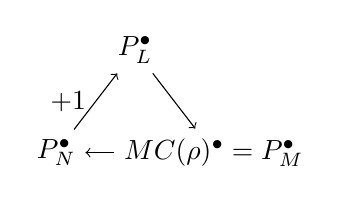
\begin{tikzpicture}[baseline=(current bounding box.center)]
    \node (L) at (1,1.3)
    {$P_L^\bullet$}; \node (N) at (0,0)
    {$P_N^\bullet$}; \node (M) at (2,0)
    {$MC(\rho)^\bullet =
      P_M^\bullet$}; \draw[->] (L) -- (M); \draw[->] (M) -- (N);
    \draw[->] (N) -- (L) node[midway, left] {$+1$};
  \end{tikzpicture}
\]
in the sense mentioned in \S{}4.1. These are the triangles giving the
homotopic category the structure of `triangulated category'. Thus, the
functor $\mathscr{P}$ allows us to construct a distinguished triangle
in $\categ{K}(\categ{P})$ starting from a `special' exact triangle
\[
  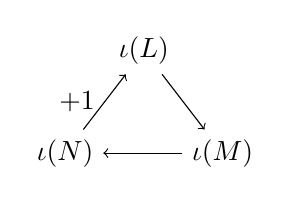
\begin{tikzpicture}[baseline=(current bounding box.center)]
    \node (L) at (1,1.3)
    {$\iota(L)$}; \node (N) at (0,0)
    {$\iota(N)$}; \node (M) at (2,0)
    {$\iota(M)$}; \draw[->] (L) -- (M); \draw[->] (M) -- (N);
    \draw[->] (N) -- (L) node[midway, left] {$+1$};
  \end{tikzpicture}
\]
in the sense of \S{}3.4. The horseshoe lemma shows that this functor
preserves as much exactness as is allowed by the context.

We should also note that once short exact sequences are lifted, we can
in fact lift every complex; this will be needed later. Here is the
precise statement:
\begin{coro}{}{coro:homol:7.9}
  Let
  \[\begin{tikzcd}[column sep=large]
      M^\bullet: & \dots \arrow[r] & M^{-3} \arrow[r] & M^{-2}
      \arrow[r] & M^{-1} \arrow[r] & M^0 \arrow[r] & 0
    \end{tikzcd}\] be a complex in an abelian category $\categ{A}$
  with enough projectives. Then there is a complex of complexes:
  \[\begin{tikzcd}[column sep=large]
      P_{M^\bullet}^\bullet: & \dots \arrow[r] & P_{M^\bullet}^{-3}
      \arrow[r] & P_{M^\bullet}^{-2} \arrow[r] & P_{M^\bullet}^{-1}
      \arrow[r] & P_{M^\bullet}^0 \arrow[r] & 0
    \end{tikzcd}\] such that each $P_{M^\bullet}^i$ is a projective
  resolution of $M^i$ and inducing $M^\bullet$ in cohomology.

  If $M^\bullet$ is exact, then $P_{M^\bullet}^\bullet$ may be chosen
  to be exact.
\end{coro}
\begin{proof}
  Break up $M^\bullet$ into short exact sequences
  \[\begin{tikzcd}
      0 \arrow[r] & K^i \arrow[r] & M^i \arrow[r] & I^{i+1} \arrow[r]
      & 0
    \end{tikzcd}\] together with exact sequences
  \[\begin{tikzcd}
      0 \arrow[r] & I^i \arrow[r] & K^i \arrow[r] & H^i \arrow[r] & 0
    \end{tikzcd}\] where $K^i$ is the kernel of $M^i \to M^{i+1}$,
  $I^{i+1}$ is its image, and $H^i$ is the cohomology at $M^i$. Choose
  arbitrary projective resolutions $P_{I^i}$, $P_{H^i}$ of $I^i$ and
  $H^i$, for all $i$. Then the horseshoe lemma
  (Lemma~\ref{lem:homol:7.8}) yields projective resolutions of $K^i$
  and short exact sequences
  \[\begin{tikzcd}
      0 \arrow[r] & P_{I^i}^\bullet \arrow[r] & P_{K^i}^\bullet
      \arrow[r] & P_{H^i}^\bullet \arrow[r] & 0,
    \end{tikzcd}\] with evident notation, and then the horseshoe lemma
  again and the previous sequences give projective resolutions
  $P_{M^i}$ of $M^i$ and short exact sequences
  \[\begin{tikzcd}
      0 \arrow[r] & P_{K^i}^\bullet \arrow[r] & P_{M^i}^\bullet
      \arrow[r] & P_{I^{i+1}}^\bullet \arrow[r] & 0.
    \end{tikzcd}\] The $P_{M^i}^\bullet$ can now be assembled into a
  sequence, by using differentials obtained by the compositions
  \[
    P_{M^i}^\bullet \to P_{I^{i+1}}^\bullet \to P_{K^{i+1}}^\bullet
    \to P_{M^{i+1}}^\bullet.
  \]
  It is clear that one obtains a complex and that
  $P_{K^{i+1}}^\bullet$, resp., $P_{I^{i+1}}^\bullet$, are the kernel,
  resp., the image, of $P_{M^i}^\bullet \to P_{M^{i+1}}^\bullet$
  (\Cref{exer:homol:1.21}). The statements follow. (If $M^\bullet$ is exact,
  then $I^i = K^i$, and the construction gives
  $P_{I^i}^\bullet = P_{K^i}^\bullet$, so that $P_{M^\bullet}^\bullet$
  is exact.)
\end{proof}

\begin{rem}{}{rem:homol:7.10}
  The proof of Corollary~\ref{coro:homol:7.9} shows that the
  resolution $P_{M^\bullet}^\bullet$, i.e.,
  \[\begin{tikzcd}[column sep=large]
      \dots \arrow[r, "d^{-4}"] & P_{M^\bullet}^{-3} \arrow[r,
      "d^{-3}"] & P_{M^\bullet}^{-2} \arrow[r, "d^{-2}"] &
      P_{M^\bullet}^{-1} \arrow[r, "d^{-1}"] & P_{M^\bullet}^0
      \arrow[r] & 0,
    \end{tikzcd}\] can in fact be chosen so that
  $\image d^i$, $\ker d^i$, and the cohomology
  $\ker d^i / \image d^{i-1}$ are all projective
  resolutions of the corresponding objects from $M^\bullet$. This is
  useful in some applications. Resolutions satisfying this property
  are called \emph{Cartan-Eilenberg} (or `fully projective')
  \emph{resolutions}.
\end{rem}

Coming back to the issue at hand, we are one step away from the
promised long exact sequence of derived functors. The last ingredient
is the following:

\begin{lem}{}{lem:homol:7.11}
  Let $\categ{A}$ be an abelian category, and let
  \[\begin{tikzcd}
      0 \arrow[r] & L^\bullet \arrow[r] & M^\bullet \arrow[r] &
      P^\bullet \arrow[r] & 0
    \end{tikzcd} \tag{$*$}\] be an exact sequence of complexes in
  $\categ{A}$, where $P^i$ is projective for all $i$. Let
  $\mathscr{F} : \categ{A} \to \categ{B}$ be any additive functor of
  abelian categories. Then the sequence obtained by applying
  $\mathscr{F}$ to $(*)$,
  \[\begin{tikzcd}
      0 \arrow[r] & \mathscr{F}(L^\bullet) \arrow[r] &
      \mathscr{F}(M^\bullet) \arrow[r] & \mathscr{F}(P^\bullet)
      \arrow[r] & 0,
    \end{tikzcd}\] is exact.
\end{lem}

Note that we are not asking $\mathscr{F}$ to be exact in any sense.

\begin{proof}
  Since $P^i$ is projective, the sequence
  \[\begin{tikzcd}
      0 \arrow[r] & L^i \arrow[r] & M^i \arrow[r] & P^i \arrow[r] & 0
    \end{tikzcd}\] splits (see the end of \ref{subsec:linrep:projectives-and-injectives}). It follows
  that
  \[\begin{tikzcd}
      0 \arrow[r] & \mathscr{F}(L^i) \arrow[r] & \mathscr{F}(M^i)
      \arrow[r] & \mathscr{F}(P^i) \arrow[r] & 0
    \end{tikzcd}\] is (split and) exact for all $i$
  (\Cref{exer:homol:5.11}). Exactness of a sequence of complexes is determined
  by exactness at each degree, so this proves the statement.
\end{proof}

Now the long exact sequence of left-derived functors is an immediate
consequence of the long exact cohomology sequence.

\begin{thm}{}{thm:homol:7.12}
  Let $\mathscr{F} : \categ{A} \to \categ{B}$ be an additive functor
  of abelian categories, and assume $\categ{A}$ has enough
  projectives. Every exact sequence
  \[\begin{tikzcd}
      0 \arrow[r] & L \arrow[r] & M \arrow[r] & N \arrow[r] & 0
    \end{tikzcd}\] in $\categ{A}$ induces a long exact sequence
  \[
    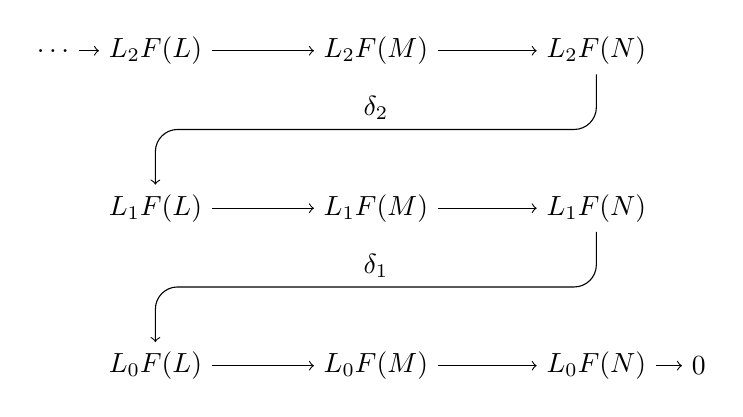
\begin{tikzpicture}[baseline=(current bounding box.center)]
      \node (dots) at (-1.3,4)
      {$\dots$}; \node (L2L) at (0,4)
      {$\categ{L}_2\mathscr{F}(L)$}; \node (L2M) at (2.8,4)
      {$\categ{L}_2\mathscr{F}(M)$}; \node (L2N) at (5.6,4)
      {$\categ{L}_2\mathscr{F}(N)$}; \node (L1L) at (0,2)
      {$\categ{L}_1\mathscr{F}(L)$}; \node (L1M) at (2.8,2)
      {$\categ{L}_1\mathscr{F}(M)$}; \node (L1N) at (5.6,2)
      {$\categ{L}_1\mathscr{F}(N)$}; \node (L0L) at (0,0)
      {$\categ{L}_0\mathscr{F}(L)$}; \node (L0M) at (2.8,0)
      {$\categ{L}_0\mathscr{F}(M)$}; \node (L0N) at (5.6,0)
      {$\categ{L}_0\mathscr{F}(N)$}; \node (zero) at (6.9,0)
      {$0$}; \draw[->] (dots) -- (L2L); \draw[->] (L2L) -- (L2M);
      \draw[->] (L2M) -- (L2N); \draw[->] (L1L) -- (L1M); \draw[->]
      (L1M) -- (L1N); \draw[->] (L0L) -- (L0M); \draw[->] (L0M) --
      (L0N); \draw[->] (L0N) -- (zero); \draw[->, rounded corners=8pt]
      (L2N.south) -- (5.6,3) -- node[above]
      {$\delta_2$} (0,3) -- (L1L.north); \draw[->, rounded
      corners=8pt] (L1N.south) -- (5.6,1) -- node[above]
      {$\delta_1$} (0,1) -- (L0L.north);
    \end{tikzpicture}
  \]
  in $\categ{B}$. Further, this assignment is covariantly functorial.
\end{thm}

The last sentence means that a morphism of short exact sequences will
induce a morphism of the corresponding long exact sequences,
compatibly with compositions. I will leave the diagram chases
necessary to prove this to the reader (\Cref{exer:homol:7.7}).

\begin{proof}
  By Lemma~\ref{lem:homol:7.8}, the given exact sequence is induced by
  an exact sequence of projective resolutions
  \[\begin{tikzcd}
      0 \arrow[r] & P_L^\bullet \arrow[r] & P_M^\bullet \arrow[r] &
      P_N^\bullet \arrow[r] & 0.
    \end{tikzcd}\] By Lemma~\ref{lem:homol:7.11}, the corresponding
  sequence
  \[\begin{tikzcd}
      0 \arrow[r] & \mathscr{F}(P_L^\bullet) \arrow[r] &
      \mathscr{F}(P_M^\bullet) \arrow[r] & \mathscr{F}(P_N^\bullet)
      \arrow[r] & 0
    \end{tikzcd}\] in $\categ{C}(\categ{B})$ is exact. As the
  cohomology objects of these complexes are precisely the left-derived
  functors of $\mathscr{F}$, the long exact cohomology sequence
  determined by this sequence (by \Cref{homol:3.5}) gives a long exact
  sequence as stated.
\end{proof}

Once more in the style of \S{}3.4, Theorem~\ref{thm:homol:7.12} tells
us that the triangle
\[
  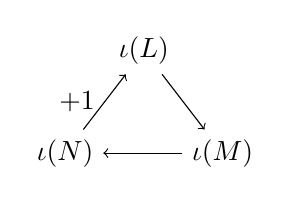
\begin{tikzpicture}[baseline=(current bounding box.center)]
    \node (L) at (1,1.3)
    {$\iota(L)$}; \node (N) at (0,0)
    {$\iota(N)$}; \node (M) at (2,0)
    {$\iota(M)$}; \draw[->] (L) -- (M); \draw[->] (M) -- (N);
    \draw[->] (N) -- (L) node[midway, left] {$+1$};
  \end{tikzpicture}
\]
induces a triangle\footnote{The indexing is potentially confusing: the
  lower $\bullet$ indicates `homological' indexing, which is opposite
  to the degree of the corresponding cochain complexes. So
  $\categ{L}_i\mathscr{F}(N)$ corresponds to degree $-i$, which is
  sent by the northeast arrow to cohomological degree $-i+1$,
  corresponding to $\categ{L}_{i-1}\mathscr{F}(L)$, as it should.}
\[
  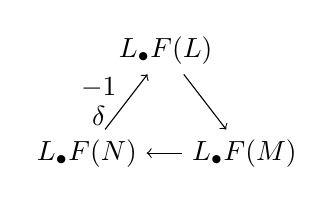
\begin{tikzpicture}[baseline=(current bounding box.center)]
    \node (L) at (1,1.3)
    {$\categ{L}_\bullet\mathscr{F}(L)$}; \node (N) at (0,0)
    {$\categ{L}_\bullet\mathscr{F}(N)$}; \node (M) at (2,0)
    {$\categ{L}_\bullet\mathscr{F}(M)$}; \draw[->] (L) -- (M);
    \draw[->] (M) -- (N); \draw[->] (N) -- (L) node[midway, left]
    {$\shortstack{$-1$ \\ $\delta$}$};
  \end{tikzpicture}
\]
The vertices of this triangle are complexes in
$\categ{C}^{\le 0} (\categ{B})$.

A completely similar situation occurs for right-derived functors: if
$\categ{A}$ has enough injectives, an exact sequence as above induces
a triangle
\[
  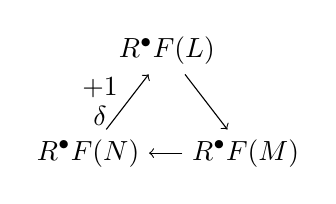
\begin{tikzpicture}[baseline=(current bounding box.center)]
    \node (L) at (1,1.3)
    {$\categ{R}^\bullet\mathscr{F}(L)$}; \node (N) at (0,0)
    {$\categ{R}^\bullet\mathscr{F}(N)$}; \node (M) at (2,0)
    {$\categ{R}^\bullet\mathscr{F}(M)$}; \draw[->] (L) -- (M);
    \draw[->] (M) -- (N); \draw[->] (N) -- (L) node[midway, left]
    {$\shortstack{$+1$ \\ $\delta$}$};
  \end{tikzpicture}
\]
where now the vertices are complexes in
$\categ{C}^{\ge 0}(\categ{B})$.

\subsection{\texorpdfstring{Relating $\mathscr{F}$,
    $\categ{L}_i\mathscr{F}$, $\categ{R}^i\mathscr{F}$}{Relating F,
    LiF, RiF}}
\label{subsec:homol:relating-f-li-f-rif}

The reader may have noticed that $\otimes$ was derived \emph{to the
  left} to obtain $\Tor$, while $\Hom$ was derived
\emph{to the right} to obtain $\operatorname{Ext}$. The asymmetry
mandating this choice lies in the fact that $\otimes$ is right-exact,
while $\Hom$ is left-exact: any additive functor can be derived to the
left or to the right (in the presence of enough projectives, resp.,
enough injectives), and the derived functors will fit in long exact
sequences as proven in Theorem~\ref{thm:homol:7.12}; but only functors
satisfying a measure of exactness can be recovered directly from their
derived versions.

To state this fact more precisely, we go back to general
considerations for the left-derived functor of an additive functor
$\mathscr{F} : \categ{A} \to \categ{B}$, where $\categ{A}$ and
$\categ{B}$ are abelian categories and $\categ{A}$ has enough
projectives, and we now assume that $\mathscr{F}$ is right-exact.

\begin{prop}{}{prop:homol:7.13}
  Let $\mathscr{F} : \categ{A} \to \categ{B}$ be a right-exact
  additive functor. Then $\categ{L}_i\mathscr{F} = 0$ for $i < 0$, and
  $\categ{L}_0\mathscr{F}$ is naturally isomorphic to $\mathscr{F}$.
\end{prop}
\begin{proof}
  Projective resolutions $P^\bullet$ of an object $M$ of $\categ{A}$
  are in $\categ{C}^{\le 0}(\categ{A})$: it follows that
  $\categ{C}(\mathscr{F})(P^\bullet)$ is $0$ in positive degree, hence
  so is its cohomology. Since $H_i = H^{-i}$ (cf. \S{}3.1), the first
  claim follows.

  As for the second, since the sequence
  \[\begin{tikzcd}
      P^{-1} \arrow[r] & P^0 \arrow[r] & M \arrow[r] & 0
    \end{tikzcd}\] is exact by construction and since $\mathscr{F}$ is
  right-exact, the sequence
  \[\begin{tikzcd}
      \mathscr{F}(P^{-1}) \arrow[r] & \mathscr{F}(P^0) \arrow[r] &
      \mathscr{F}(M) \arrow[r] & 0
    \end{tikzcd}\] is exact. This induces an isomorphism
  $\nu_L : \categ{L}_0\mathscr{F}(M) =
  H^0(\categ{C}(\mathscr{F})(P^\bullet)) \xrightarrow{\sim}
  \mathscr{F}(M)$.

  If $\varphi : M_0 \to M_1$ is a morphism in $\categ{A}$, by
  Proposition~\ref{prop:homol:6.5} there exists a morphism of
  projective resolutions
  $\alpha^\bullet : P_0^\bullet \to P_1^\bullet$ inducing $\varphi$:
  there is a commutative diagram
  \[\begin{tikzcd}
      \dots \arrow[r] & P_0^{-1} \arrow[r] \arrow[d, "\alpha^{-1}"] &
      P_0^0 \arrow[r] \arrow[d, "\alpha^0"] & M_0 \arrow[r]
      \arrow[d, "\varphi"] & 0 \\
      \dots \arrow[r] & P_1^{-1} \arrow[r] & P_1^0 \arrow[r] & M_1
      \arrow[r] & 0
    \end{tikzcd}\] and $H^0(\alpha^\bullet)$ agrees with
  $\varphi$. Applying $\mathscr{F}$ and truncating, we get a
  commutative diagram
  \[\begin{tikzcd}
      \mathscr{F}(P_0^{-1}) \arrow[r] \arrow[d,
      "\mathscr{F}(\alpha^{-1})"] & \mathscr{F}(P_0^0) \arrow[r]
      \arrow[d, "\mathscr{F}(\alpha^0)"] &
      \mathscr{F}(M_0) \arrow[r] \arrow[d, "\mathscr{F}(\varphi)"] & 0 \\
      \mathscr{F}(P_1^{-1}) \arrow[r] & \mathscr{F}(P_1^0) \arrow[r] &
      \mathscr{F}(M_1) \arrow[r] & 0
    \end{tikzcd}\] with exact rows since $\mathscr{F}$ is
  right-exact. It follows that the diagram
  \[\begin{tikzcd}
      \categ{L}_0\mathscr{F}(M_0) \arrow[r,
      "\categ{L}_0\mathscr{F}(\varphi)"] \arrow[d, "\nu_{M_0}"',
      "\sim"] & \categ{L}_0\mathscr{F}(M_1)
      \arrow[d, "\sim", "\nu_{M_1}"'] \\
      \mathscr{F}(M_0) \arrow[r, "\mathscr{F}(\varphi)"'] &
      \mathscr{F}(M_1)
    \end{tikzcd}\] commutes, proving that
  $\nu : \categ{L}_0\mathscr{F} \to \mathscr{F}$ is a natural
  isomorphism.
\end{proof}
Going back to Theorem~\ref{thm:homol:7.12}, we see that if
$\mathscr{F}$ is right-exact, then the tail end of the long exact
sequence of left-derived functors for $\mathscr{F}$ consists of an
application of $\mathscr{F}$ itself. Thus, the situation in this case
is the following: starting from a short exact sequence
\[\begin{tikzcd}
    0 \arrow[r] & L \arrow[r] & M \arrow[r] & N \arrow[r] & 0
  \end{tikzcd}\] in $\categ{A}$, we apply $\mathscr{F}$ to obtain an
exact sequence
\[\begin{tikzcd}
    \mathscr{F}(L) \arrow[r] & \mathscr{F}(M) \arrow[r] &
    \mathscr{F}(N) \arrow[r] & 0
  \end{tikzcd}\] in which we lost `the $0$ on the left'. The long
exact sequence saves the day, continuing the new sequence into an
exact complex:
\[
  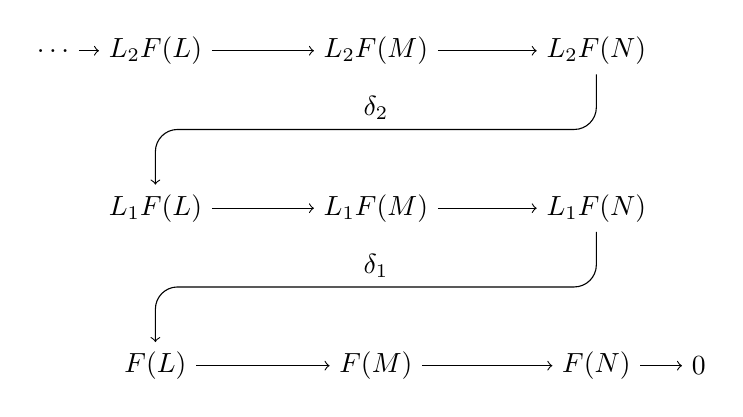
\begin{tikzpicture}[baseline=(current bounding box.center)]
    \node (dots) at (-1.3,4)
    {$\dots$}; \node (L2L) at (0,4)
    {$\categ{L}_2\mathscr{F}(L)$}; \node (L2M) at (2.8,4)
    {$\categ{L}_2\mathscr{F}(M)$}; \node (L2N) at (5.6,4)
    {$\categ{L}_2\mathscr{F}(N)$}; \node (L1L) at (0,2)
    {$\categ{L}_1\mathscr{F}(L)$}; \node (L1M) at (2.8,2)
    {$\categ{L}_1\mathscr{F}(M)$}; \node (L1N) at (5.6,2)
    {$\categ{L}_1\mathscr{F}(N)$}; \node (FL) at (0,0)
    {$\mathscr{F}(L)$}; \node (FM) at (2.8,0)
    {$\mathscr{F}(M)$}; \node (FN) at (5.6,0)
    {$\mathscr{F}(N)$}; \node (zero) at (6.9,0)
    {$0$}; \draw[->] (dots) -- (L2L); \draw[->] (L2L) -- (L2M);
    \draw[->] (L2M) -- (L2N); \draw[->] (L1L) -- (L1M); \draw[->]
    (L1M) -- (L1N); \draw[->] (FL) -- (FM); \draw[->] (FM) -- (FN);
    \draw[->] (FN) -- (zero); \draw[->, rounded corners=8pt]
    (L2N.south) -- (5.6,3) -- node[above]
    {$\delta_2$} (0,3) -- (L1L.north); \draw[->, rounded corners=8pt]
    (L1N.south) -- (5.6,1) -- node[above]
    {$\delta_1$} (0,1) -- (FL.north);
  \end{tikzpicture}
\]
That is, $\categ{L}_1\mathscr{F}$ measures the extent to which
$\mathscr{F}$ fails to be left-exact, and the higher
$\categ{L}_i\mathscr{F}$ give further measures of this failure.

Similarly, $\categ{R}^0\mathscr{F}$ is naturally isomorphic to
$\mathscr{F}$ if $\mathscr{F}$ is left-exact. In this case, applying
$\mathscr{F}$ to the original sequence gives the exact sequence
\[\begin{tikzcd}
    0 \arrow[r] & \mathscr{F}(L) \arrow[r] & \mathscr{F}(M) \arrow[r]
    & \mathscr{F}(N)
  \end{tikzcd}\] where we lost the $0$ on the right; the job of the
right-derived functors of $\mathscr{F}$ is to extend this sequence to
an exact complex
\[
  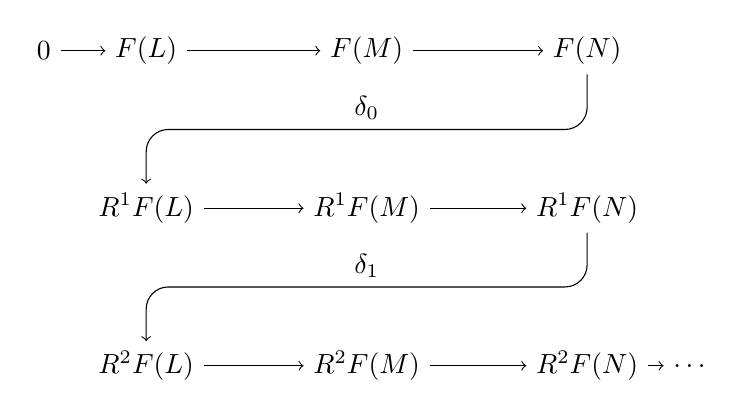
\begin{tikzpicture}[baseline=(current bounding box.center)]
    \node (zero) at (-1.3,4)
    {$0$}; \node (FL) at (0,4)
    {$\mathscr{F}(L)$}; \node (FM) at (2.8,4)
    {$\mathscr{F}(M)$}; \node (FN) at (5.6,4)
    {$\mathscr{F}(N)$}; \node (R1L) at (0,2)
    {$\categ{R}^1\mathscr{F}(L)$}; \node (R1M) at (2.8,2)
    {$\categ{R}^1\mathscr{F}(M)$}; \node (R1N) at (5.6,2)
    {$\categ{R}^1\mathscr{F}(N)$}; \node (R2L) at (0,0)
    {$\categ{R}^2\mathscr{F}(L)$}; \node (R2M) at (2.8,0)
    {$\categ{R}^2\mathscr{F}(M)$}; \node (R2N) at (5.6,0)
    {$\categ{R}^2\mathscr{F}(N)$}; \node (dots) at (6.9,0)
    {$\dots$}; \draw[->] (zero) -- (FL); \draw[->] (FL) -- (FM);
    \draw[->] (FM) -- (FN); \draw[->] (R1L) -- (R1M); \draw[->] (R1M)
    -- (R1N); \draw[->] (R2L) -- (R2M); \draw[->] (R2M) -- (R2N);
    \draw[->] (R2N) -- (dots); \draw[->, rounded corners=8pt]
    (FN.south) -- (5.6,3) -- node[above]
    {$\delta_0$} (0,3) -- (R1L.north); \draw[->, rounded corners=8pt]
    (R1N.south) -- (5.6,1) -- node[above]
    {$\delta_1$} (0,1) -- (R2L.north);
  \end{tikzpicture}
\]
No identification of $\mathscr{F}$ with any of its derived functors
should be expected if $\mathscr{F}$ does not satisfy some exactness
property. If $\mathscr{F}$ is exact on the nose, then both
$\categ{L}_0\mathscr{F}$ and $\categ{R}^0\mathscr{F}$ agree with
$\mathscr{F}$ (up to natural isomorphism); but this is no cause for
great excitement, since all other $\categ{L}_i\mathscr{F}$,
$\categ{R}^i\mathscr{F}$ vanish in this case (\Cref{exer:homol:7.8}). As
already pointed out in Example~\ref{exam:homol:7.2}, one should not
expect to learn anything new from an exact functor by deriving it.

\subsection{Example: A little group cohomology}
\label{subsec:homol:example-a-little-group-cohomology}

In the beginning of this chapter I pointed out that the general
strategy informing the development of homological algebra has numerous
applications and I mentioned group and sheaf cohomology as
examples. Here are a few words on group cohomology (sheaf cohomology
would take us too far).

How do we extract `cohomological invariants' from a group $G$?
Consider the category $G\text{-}\categ{Mod}$ of abelian groups endowed
with a left-$G$-action, equivalently, the category of
left-$\Z[G]$-modules, where $\Z[G]$ is the group ring briefly
encountered in \ref{subsec:rings:monoid-rings}. Objects of $G\text{-}\categ{Mod}$ may be
called $G$-modules.

For a $G$-module $M$, $M^G$ denotes the set of elements that are fixed
under the action of $G$: these are reasonably called the
\emph{invariants} of the action. Note that $M^G$ is an abelian group
carrying a trivial action of $G$; it is clear that setting $M \to M^G$
defines a covariant functor
$\cdot^G : G\text{-}\categ{Mod} \to \categ{Ab}$. Both
$G\text{-}\categ{Mod}$ and $\categ{Ab}$ are abelian categories, and it
takes a moment to realize that $\cdot^G$ is a left-exact functor: the
reader should either check this directly or do \Cref{exer:homol:7.16} and then
remember \Cref{linrep:1.19}. The reader should in fact contemplate why
this functor is not right-exact: if $G$ acts trivially on a coset
$[m]$ of a quotient $M/L$, there is no reason \emph{a priori} why $G$
should act trivially on a representative $m$.

We would have drawn this conclusion without difficulty before delving
into homological algebra. Homological algebra tells us how to address
this type of situation and `quantify' precisely the failure of
exactness, by means of an appropriate derived functor.

The $i$-th right-derived functor of $\cdot^G$ is denoted $H^i(G,
\_)$. Therefore, $H^0(G, M) = M^G$, and for every short exact sequence
of $G$-modules
\[\begin{tikzcd}
    0 \arrow[r] & L \arrow[r] & M \arrow[r] & N \arrow[r] & 0
  \end{tikzcd}\] we obtain (from Theorem~\ref{thm:homol:7.12}) a long
exact sequence of abelian groups:
\[\begin{tikzcd}
    0 \arrow[r] & L^G \arrow[r] & M^G \arrow[r] & N^G \arrow[r] &
    H^1(G, L) \arrow[r] & H^1(G, M) \arrow[r] & \dots
  \end{tikzcd}\] Note that $M^G = \Hom_{\Z[G]}(\Z, M)$, where $\Z$ is
given the trivial module structure. Thus,
$H^i(G, M) = \operatorname{Ext}^i_{\Z[G]}(\Z, M)$; as we know already
(and as will finally be verified in \S{}8), this can be computed by an
injective resolution of $M$ or by a projective resolution of $\Z$.
\begin{exam}{}{exam:homol:7.14}
  Take $G = \Z$. Then $\Z[G]$ is the ring $\Z[x,x^{-1}]$ of Laurent
  polynomials. As $\Z[x,x^{-1}]/(1-x) \cong \Z$, with the trivial
  action (check this!), the complex
  \[\begin{tikzcd}
      \dots \arrow[r] & 0 \arrow[r] & \Z[x,x^{-1}] \arrow[r,
      "\cdot(1-x)"] & \Z[x,x^{-1}] \arrow[r] & 0 \arrow[r] & \dots
    \end{tikzcd}\] is a free, hence projective, resolution of $\Z$,
  endowed with the trivial $\Z$-action. Applying the (contravariant)
  $\Hom_{\Z[x,x^{-1}]}(\_, M)$, we see that $H^\bullet(\Z, M)$ is
  computed by the cohomology of
  \[\begin{tikzcd}
      \dots \arrow[r] & 0 \arrow[r] & M \arrow[r, "\cdot(1-x)"] & M
      \arrow[r] & 0 \arrow[r] & \dots
    \end{tikzcd}\] `Multiplication by $x$' on $M$ is nothing but the
  action of the generator of $G = \Z$. We conclude that
  \[
    H^0(\Z, M) = \ker\bigl(M \xrightarrow{\cdot(1-x)} M\bigr) = M^{\Z}
  \]
  (as we knew already),
  \[
    H^1(\Z, M) = \frac{M}{(1-x)M},
  \]
  and $H^i(\Z, M) = 0$ for all $i < 0$ and $i \ge 2$.
\end{exam}

\begin{exam}{Finite cyclic groups}{exam:homol:7.15}
  Let $G = C_m$ be a cyclic group of order $m$; then
  $\Z[G] \cong \Z[x]/(x^m - 1)$. Again it is not difficult to produce
  a projective resolution of $\Z$ (with trivial action) in the
  category of $\Z[C_m]$-modules: letting
  $N = 1 + x + \dots + x^{m-1} = (1 - x^m)/(1 - x)$, the reader will
  verify that the complex
  \[\begin{tikzcd}
      \dots \arrow[r, "\cdot N"] & \Z[C_m] \arrow[r, "\cdot(1-x)"] &
      \Z[C_m] \arrow[r, "\cdot N"] & \Z[C_m] \arrow[r, "\cdot(1-x)"] &
      \Z[C_m] \arrow[r] & 0 \arrow[r] & \dots
    \end{tikzcd}\] has cohomology $\cong \Z$, concentrated in degree
  $0$ (i.e., on the last nonzero term). Applying
  $\Hom_{\Z[C_m]}(\_, M)$, we get the complex
  \[\begin{tikzcd}
      \dots \arrow[r] & 0 \arrow[r] & M \arrow[r, "\cdot(1-x)"] & M
      \arrow[r, "\cdot N"] & M \arrow[r, "\cdot(1-x)"] & M \arrow[r,
      "\cdot N"] & \dots
    \end{tikzcd}\] and deduce that $H^i(C_m, M) = 0$ for $i < 0$,
  $H^0(C_m, M) = M^{C_m}$, and for all $i > 0$
  \[
    H^{2i+1}(C_m, M) \cong \frac{\ker\bigl(M \xrightarrow{\cdot N}
      M\bigr)}{(1-x)M},
  \]
  \[
    H^{2i}(C_m, M) \cong \frac{M^{C_m}}{N \cdot M}.
  \]
\end{exam}
There is a standard free resolution of $\Z$ over a group ring $\Z[G]$,
which leads to a concrete description of group cohomology.  For a
finite group $G$, of order $m$, the beginning of this resolution goes
as follows. Consider the complex
\[\begin{tikzcd}[column sep=large]
    (\dagger) & \dots \arrow[r] & \Z[G]^{m^2} \arrow[r, "d^{-2}"] &
    \Z[G]^m \arrow[r, "d^{-1}"] & \Z[G] \arrow[r, "d^0"] & \Z
    \arrow[r] & 0 \arrow[r] & \dots
  \end{tikzcd}\] Here, a basis of $\Z[G]^{m^k}$ over $\Z[G]$ consists
of $k$-tuples $[g_1, \dots, g_k]$ of elements of $G$. The morphisms in
$(\dagger)$ are defined by setting
\[
  d^{-1}([g]) = 1 \cdot g - 1 \cdot e_G \in \Z[G], \qquad d^{-2}([g_1,
  g_2]) = g_1[g_2] - [g_1g_2] + [g_1],
\]
on the bases and extending by $\Z[G]$-linearity, and $d^0$ sends every
$g \in G$ to $1$, so that
$d^0\bigl(\sum_{g \in G} a_g g\bigr) = \sum_{g \in G} a_g$. (Needless
to say, $d^{-k}$ may be defined for all $k$.) The reader will check
that $(\dagger)$ is exact (\Cref{exer:homol:7.17}), at least for the part
relevant to the discussion that follows. Therefore,
\[\begin{tikzcd}[column sep=large]
    \dots \arrow[r] & \Z[G]^{m^2} \arrow[r, "d^{-2}"] & \Z[G]^m
    \arrow[r, "d^{-1}"] & \Z[G] \arrow[r] & 0 \arrow[r] & \dots
  \end{tikzcd}\] is (the beginning of) a free $\Z[G]$-resolution of
$\Z$ (endowed with the trivial $G$-action), and group cohomology can
be computed as the cohomology of the complex obtained by applying
$\Hom_{\Z[G]}(\_, M)$ to this resolution:
\[\begin{tikzcd}[column sep=large]
    0 \arrow[r] & \Hom_{\Z[G]}(\Z[G], M) \arrow[r] &
    \Hom_{\Z[G]}(\Z[G]^m, M) \arrow[r] & \Hom_{\Z[G]}(\Z[G]^{m^2}, M)
    \arrow[r] & \dots
  \end{tikzcd}\] Here, $\Hom_{\Z[G]}(\Z[G]^{m^k}, M) \cong M^{m^k}$
may be identified with the abelian group of functions $G^k \to M$,
since every $\Z[G]$-linear map $\Z[G]^{m^k} \to M$ is determined by
its action on a basis. Denote this abelian group by $C^k(G, M)$: this
is the group of $k$-cochains of $G$ with values in $M$.

We can now summarize what we have found as follows:

\begin{prop}{}{prop:homol:7.16}
  Let $G$ be a finite group, and let $M$ be a $G$-module. Then the
  group cohomology $H^i(G, M)$ is the cohomology of the cochain
  complex induced by $(\dagger)$:
  \[\begin{tikzcd}
      0 \arrow[r] & C^0(G, M) \arrow[r, "d_G^0"] & C^1(G, M) \arrow[r,
      "d_G^1"] & C^2(G, M) \arrow[r, "d_G^2"] & \dots
    \end{tikzcd}\]
\end{prop}

Tracing definitions, we see that for $a \in C^0(G, M) = M$ and
$\alpha : G \to M$ in $C^1(G, M)$,
\[
  d_G^0(a)(g) = ga - a, \qquad d_G^1(\alpha)(g_1, g_2) =
  g_1\alpha(g_2) - \alpha(g_1g_2) + \alpha(g_1).
\]
\begin{exam}{}{exam:homol:7.17}
  Let $G$ be the Galois group of a finite Galois extension
  $k \subseteq F$. Then $G$ acts on the multiplicative group $F^*$ of
  $F$, and we can view $F^*$ as a $G$-module.
\end{exam}

\begin{prop}{Hilbert's theorem 90}{prop:homol:7.18}
  $H^1(G, F^*) = 0$.
\end{prop}

Indeed, with notation as above we have
$H^1(G, F^*) \cong \ker d_G^1 / \image d_G^0$, and we can
compute this quotient explicitly. Let $\alpha \in C^1(G, F^*)$; denote
by $\alpha_g$ the image of $g$ in $F^*$ by $\alpha$. The `cocycle
condition' $\alpha \in \ker d_G^1$ translates into
\[
  \alpha_{gh} = \alpha_g \cdot g(\alpha_h)
\]
for all $g, h$ in $G$. (I am now writing the operation in $F^*$
multiplicatively and viewing elements of $G$ as automorphisms of $F$.)

The elements $h \in G$ are pairwise distinct as automorphisms of $F$,
so by \Cref{fields:exer:6.14} they must be linearly independent.  Therefore,
there exists a $\gamma \in F$ such that
\[
  \beta := \sum_{h \in G} \alpha_h \cdot h(\gamma) \ne 0.
\]
Thus $\beta \in F^*$, and for all $g \in G$
\[
  g(\beta) = \sum_{h \in G} g(\alpha_h) \cdot (gh)(\gamma)
  \overset{!}{=} \sum_{h \in G} \alpha_g^{-1} \alpha_{gh} \cdot
  (gh)(\gamma) = \alpha_g^{-1} \beta
\]
where the equality marked $\overset{!}{=}$ holds by the cocycle
condition. That is, we have found that there exists a $\beta \in F^*$
such that
\[
  \alpha_g = \frac{\beta}{g(\beta)}
\]
for all $g \in G$. But this says precisely that $\alpha$ is in the
image of $d_G^0$, proving that
$\ker d_G^1 / \image d_G^0 = 0$, as claimed.

Claim~\ref{prop:homol:7.18} is significant: it goes under the name of
\emph{Hilbert's theorem 90}, because in the case in which $G$ is the
Galois group of a finite cyclic extension, it recovers precisely the
classical result with this name. The reader had the opportunity to
prove this particular case in \Cref{fields:exer:6.16} and now will enjoy the
chance to verify that indeed Claim~\ref{prop:homol:7.18} implies
Hilbert's result (\Cref{exer:homol:7.18}).

Group cohomology is a useful tool in algebraic number theory,
algebraic topology, and other fields, and so is the companion `group
homology' $H_\bullet(G, M)$, defined analogously by the left-derived
functors of the functor $\cdot_G$ associating with every $G$-module
$M$ the module
\[
  M_G := \frac{M}{\langle gm - m \rangle_{g \in G}}
\]
(just as the elements of $M^G$ are called invariants, elements of
$M_G$ are called \emph{coinvariants} of the action). For example, in
Example~\ref{exam:homol:7.14} we verified that
$H^1(\Z, M) = M_{\Z} = H_0(\Z, M)$. The reader should now have no
difficulty computing simple examples, such as the homology
$H_\bullet(\Z, M)$ (\Cref{exer:homol:7.19}).

\subsection*{Exercises}

\begin{exer}{\exerused{}}{exer:homol:7.1}
  Let $\mathscr{T} : \categ{Ab} \to \categ{Ab}$ be the additive
  functor defined by tensoring by $\Z/2\Z$:
  $\mathscr{T}(A) := A \otimes_\Z \Z/2\Z$. Prove that no nontrivial
  projective abelian groups can be written as $\mathscr{T}(P)$, for
  any abelian group $P$. [\S{}\ref{subsec:homol:viewpoint-shift}]
\end{exer}
\begin{exer}{}{exer:homol:7.2}
  Let $\categ{A}$, $\categ{B}$ be abelian categories, let
  $\mathscr{F} : \categ{A} \to \categ{B}$ be an additive functor, and
  let
  $\categ{C}(\mathscr{F}) : \categ{C}(\categ{A}) \to
  \categ{C}(\categ{B})$ be the corresponding functor of complexes.  If
  $\alpha^\bullet : L^\bullet \to M^\bullet$ is a morphism in
  $\categ{C}(\categ{A})$, prove that $\categ{C}(\mathscr{F})$ sends
  the mapping cone of $\alpha^\bullet$ to the mapping cone of
  $\categ{C}(\mathscr{F})(\alpha^\bullet)$.
\end{exer}
\begin{exer}{\exerused{}}{exer:homol:7.3}
  With notation as in \Cref{prop:homol:7.3}, prove that the natural
  transformation
  $\categ{L}\mathscr{F} \circ \mathscr{P}_{\categ{A}} \rightsquigarrow
  \mathscr{P}_{\categ{B}} \circ \categ{K}(\mathscr{F})$ is not
  necessarily an isomorphism. (Hint: View the quasi-isomorphism in
  \Cref{homol:4.6} as a projective resolution in $\Z\text{-}\categ{Mod}$,
  and take
  $\mathscr{F} : \Z\text{-}\categ{Mod} \to
  (\Z/2\Z)\text{-}\categ{Mod}$ to be $\_\otimes_\Z (\Z/2\Z)$.)
  [\S{}\ref{subsec:homol:universal-property-of-the-derived-functor}]
\end{exer}
\begin{exer}{\exerused{}}{exer:homol:7.4}
  (Cf.\ \Cref{rem:homol:7.4}.) Let $\categ{A}$, $\categ{B}$, $\categ{C}$ be
  abelian categories, and let $\mathscr{F} : \categ{A} \to \categ{B}$,
  $\mathscr{G} : \categ{B} \to \categ{C}$ be additive functors. Assume
  that $\categ{A}$ and $\categ{B}$ have enough projectives, so that
  the derived functors $\categ{L}\mathscr{F}$ and
  $\categ{L}\mathscr{G}$ are defined, as well as the derived functor
  $\categ{L}(\mathscr{G} \circ \mathscr{F})$. Further, assume that
  $\mathscr{F}$ maps projective objects to projective objects. Prove
  that $\categ{L}\mathscr{G} \circ \categ{L}\mathscr{F}$ and
  $\categ{L}(\mathscr{G} \circ \mathscr{F})$ are naturally
  isomorphic. [\S{}\ref{subsec:homol:universal-property-of-the-derived-functor}]
\end{exer}
\begin{exer}{\exerused{}}{exer:homol:7.5}
  With notation as in \Cref{lem:homol:7.8}, show that there is a morphism
  $\rho^\bullet : P_N[-1]^\bullet \to P_L^\bullet$ such that
  $P_M^\bullet$ is homotopy equivalent to the mapping cone
  $MC(\rho)^\bullet$. (Hint: Look at the proof of the lemma; use the
  differentials $P_L^i \oplus P_N^i \to P_L^{i+1} \oplus P_N^{i+1}$ to
  define morphisms $P_N^i \to P_L^{i+1}$.) [\S{}\ref{subsec:homol:relating-f-li-f-rif}]
\end{exer}
\begin{exer}{$\lnot$}{exer:homol:7.6}
  Let $\categ{B}$, $\categ{C}$ be abelian categories, and assume
  $\categ{B}$ has enough projectives, so that Cartan-Eilenberg
  resolutions can be constructed, as in \Cref{coro:homol:7.9} (cf.\ also
  \Cref{rem:homol:7.10}). Let $\mathscr{G} : \categ{B} \to \categ{C}$ be an
  additive functor, and let
  $M^\bullet : \dots \to M^{-2} \to M^{-1} \to M^0 \to 0$ be a complex
  in $\categ{B}$. Let
  $P_{M^\bullet}^\bullet : \dots \to P_{M^\bullet}^{-2} \to
  P_{M^\bullet}^{-1} \to P_{M^\bullet}^0 \to 0$ be a Cartan-Eilenberg
  resolution of $M^\bullet$. Prove that $\mathscr{G}$ maps the
  cohomology of this complex isomorphically to the cohomology of the
  complex
  $\dots \to \mathscr{G}(P_{M^\bullet}^{-2}) \to
  \mathscr{G}(P_{M^\bullet}^{-1}) \to \mathscr{G}(P_{M^\bullet}^0) \to
  0$. (Hint: With notation as in the proof of \Cref{coro:homol:7.9}, for all
  $i$ and $j$ we have exact sequences
  $0 \to P_{K^j}^i \to P_{M^j}^i \to P_{I^{j+1}}^i \to 0$ and
  $0 \to P_{I^j}^i \to P_{K^j}^i \to P_{H^j}^i \to 0$. Note that these
  necessarily split.)

  Stenographically,
  $\mathscr{G}(H^q(P_{M^\bullet}^\bullet)) \cong
  H^q(\mathscr{G}(P_{M^\bullet}^\bullet))$, where cohomology is
  computed with respect to the $M$-degree. Also note that, by
  construction, $H^q(P_{M^\bullet}^\bullet)$ is a projective
  resolution of $H^q(M^\bullet)$; cf.\ \Cref{rem:homol:7.10}. This will be an
  ingredient in the comparison of derived functors for the composition
  of two functors by means of spectral sequences; cf.\ Exercises~8.8
  and 9.10. [\ref{exer:homol:9.10}]
\end{exer}
\begin{exer}{\exerused{}}{exer:homol:7.7}
  Complete the proof of Theorem~\ref{thm:homol:7.12} by showing that
  morphisms of short exact sequences induce morphisms of the
  corresponding long exact sequences of derived functors. [\S{}\ref{subsec:homol:long-exact-sequence-of-derived-functors}]
\end{exer}
\begin{exer}{\exerused{}}{exer:homol:7.8}
  Let $\categ{A}$, $\categ{B}$ be abelian categories, and let
  $\mathscr{F} : \categ{A} \to \categ{B}$ be an exact functor.  Assume
  $\categ{A}$ has both enough projectives and enough injectives, so
  that $\categ{L}_i\mathscr{F}$ and $\categ{R}^i\mathscr{F}$ are both
  defined. Prove that $\categ{L}_i\mathscr{F}$ and
  $\categ{R}^i\mathscr{F}$ are both the zero functor for $i \ne
  0$. [\S{}\ref{subsec:homol:relating-f-li-f-rif}]
\end{exer}
\begin{exer}{\exerused{}}{exer:homol:7.9}
  Let $\categ{A}$, $\categ{B}$ be abelian categories, and let
  $\mathscr{F} : \categ{A} \to \categ{B}$ be an additive functor.
  Assume $\categ{A}$ has enough projectives, so that
  $\categ{L}_i\mathscr{F}$ is defined. Prove that if $P$ is
  projective, then $\categ{L}_0\mathscr{F}(P) \cong \mathscr{F}(P)$
  and $\categ{L}_i\mathscr{F}(P) = 0$ for $i \ne 0$. [\S{}\ref{subsec:homol:resolution-by-acyclic-objects}]
\end{exer}
\begin{exer}{}{exer:homol:7.10}
  Let $\categ{A}$, $\categ{B}$ be abelian categories, and let
  $\mathscr{F} : \categ{A} \to \categ{B}$ be an additive functor.
  Assume $\categ{A}$ has enough projectives, so that
  $\categ{L}_i\mathscr{F}$ is defined. Prove that
  $\categ{L}_0(\mathscr{F})$ is a right-exact functor, determining the
  same higher derived functors $\categ{L}_i$, $i > 0$, as
  $\mathscr{F}$.
\end{exer}
\begin{exer}{$\lnot$}{exer:homol:7.11}
  Let $\categ{A}$, $\categ{B}$ be abelian categories, and let
  $\mathscr{F} : \categ{A} \to \categ{B}$ be an additive functor;
  assume $\categ{A}$ has enough projectives. Let
  \[\begin{tikzcd}
      0 \arrow[r] & K \arrow[r] & P \arrow[r] & A \arrow[r] & 0
    \end{tikzcd}\] be a short exact sequence in $\categ{A}$, with $P$
  projective.  Prove that
  $\categ{L}_i\mathscr{F}(A) \cong \categ{L}_{i-1}\mathscr{F}(K)$, for
  all $i > 1$. [\ref{exer:homol:7.12}]
\end{exer}
\begin{exer}{\exerused{}}{exer:homol:7.12}
  Generalize Exercise~\ref{exer:homol:7.11} as follows: with the same
  notation, assume
  \[\begin{tikzcd}
      0 \arrow[r] & K \arrow[r] & B^{-k} \arrow[r] & \dots \arrow[r] &
      B^{-1} \arrow[r] & A \arrow[r] & 0
    \end{tikzcd}\] is an exact sequence in $\categ{A}$, such that
  $\categ{L}_i\mathscr{F}(B^{-j}) = 0$ for $i > 0$, $1 \le j \le k$.
  Prove that
  $\categ{L}_i\mathscr{F}(A) \cong \categ{L}_{i-k}\mathscr{F}(K)$, for
  all $i > k$. [\S{}\ref{subsec:homol:resolution-by-acyclic-objects}, \ref{exer:homol:8.11}]
\end{exer}
\begin{exer}{$\lnot$}{exer:homol:7.13}
  Let $\categ{A}$, $\categ{B}$ be abelian categories. A collection of
  functors $\mathscr{T}^i : \categ{A} \to \categ{B}$, $i \ge 0$, is
  called a (`cohomological') $\delta$-functor if
  \begin{itemize}
  \item every short exact sequence
    \[\begin{tikzcd}
        (\dagger) & 0 \arrow[r] & L \arrow[r] & M \arrow[r] & N
        \arrow[r] & 0
      \end{tikzcd}\] in $\categ{A}$ determines `connecting morphisms'
    \[
      \delta^i : \mathscr{T}^i(N) \to \mathscr{T}^{i+1}(L)
    \]
    such that the induced sequence
    \[
      (\ddagger) \quad
      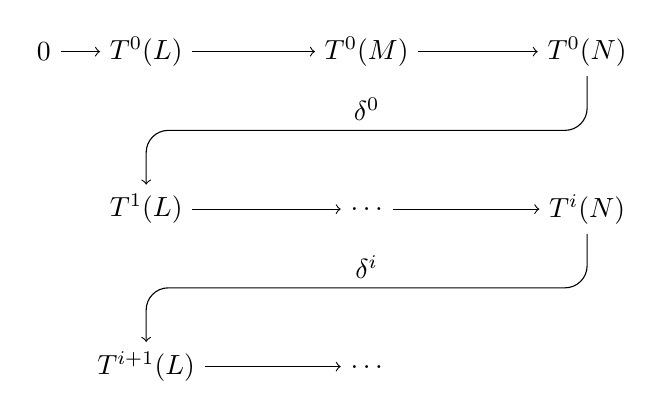
\begin{tikzpicture}[baseline=(current bounding box.center)]
        \node (zero) at (-1.3,4)
        {$0$}; \node (T0L) at (0,4)
        {$\mathscr{T}^0(L)$}; \node (T0M) at (2.8,4)
        {$\mathscr{T}^0(M)$}; \node (T0N) at (5.6,4)
        {$\mathscr{T}^0(N)$}; \node (T1L) at (0,2)
        {$\mathscr{T}^1(L)$}; \node (dots1) at (2.8,2)
        {$\dots$}; \node (TiN) at (5.6,2)
        {$\mathscr{T}^i(N)$}; \node (Ti1L) at (0,0)
        {$\mathscr{T}^{i+1}(L)$}; \node (dots2) at (2.8,0)
        {$\dots$}; \draw[->] (zero) -- (T0L); \draw[->] (T0L) --
        (T0M); \draw[->] (T0M) -- (T0N); \draw[->] (T1L) -- (dots1);
        \draw[->] (dots1) -- (TiN); \draw[->] (Ti1L) -- (dots2);
        \draw[->, rounded corners=8pt] (T0N.south) -- (5.6,3) --
        node[above]
        {$\delta^0$} (0,3) -- (T1L.north); \draw[->, rounded
        corners=8pt] (TiN.south) -- (5.6,1) -- node[above]
        {$\delta^i$} (0,1) -- (Ti1L.north);
      \end{tikzpicture}
    \]
    is exact;
  \item the assignment of a complex $(\ddagger)$ for every short exact
    sequence $(\dagger)$ is functorial (in the sense specified in
    \Cref{exer:homol:3.11}).
  \end{itemize}
  Prove that for every additive functor
  $\mathscr{F} : \categ{A} \to \categ{B}$, the derived functors
  $\categ{R}^i\mathscr{F}$, $i \ge 0$, form a cohomological
  $\delta$-functor. Prove that cohomology itself is a $\delta$-functor
  from $\categ{C}^{\ge 0}(\categ{A})$ to $\categ{A}$.

  Define a notion of `homological' $\delta$-functor
  $\{\mathscr{T}_i\}$, and prove that left-derived functors give an
  example. [\ref{exer:homol:7.14}, \ref{exer:homol:8.14}]
\end{exer}
\begin{exer}{$\lnot$}{exer:homol:7.14}
  `Morphisms' $\{\mathscr{T}^i\} \to \{\mathscr{S}^i\}$ of
  $\delta$-functors (Exercise~\ref{exer:homol:7.13}) are natural
  transformations of the individual functors $\mathscr{T}^i$,
  $\mathscr{S}^i$ that induce morphisms of the corresponding long
  exact sequences $(\ddagger)$, for every short exact sequence
  $(\dagger)$ (in other words, that preserve the connecting morphisms
  $\delta$).

  A $\delta$-functor $\{\mathscr{T}^i\}$ is \emph{universal} if for
  every $\delta$-functor $\{\mathscr{S}^i\}$, every natural
  transformation $\mathscr{T}^0 \rightsquigarrow \mathscr{S}^0$
  extends to a unique morphism of $\delta$-functors
  $\{\mathscr{T}^i\} \to \{\mathscr{S}^i\}$.

  Universal $\delta$-functors are of course unique up to isomorphism.

  It is not hard (but it involves a fair number of diagram chases) to
  show that a $\delta$-functor $\{\mathscr{T}^i\}$ is universal if for
  every $i > 0$ and every object $A$ of $\categ{A}$ there exists a
  monomorphism $\iota : A \to B$ for some $B$, such that
  $\mathscr{T}^i(\iota) = 0$. This makes each $\mathscr{T}^i$,
  $i > 0$, \emph{effaceable}. Figure out how the proof begins: assume
  that $\{\mathscr{T}^i\}$ and $\{\mathscr{S}^i\}$ are
  $\delta$-functors and that $\mathscr{T}^1$ is effaceable; show how
  to extend a natural transformation
  $\mathscr{T}^0 \rightsquigarrow \mathscr{S}^0$ to a natural
  transformation $\mathscr{T}^1 \rightsquigarrow \mathscr{S}^1$,
  compatibly with the connecting morphisms. (Hint: If $\mathscr{T}^1$
  is effaced by $\iota : A \to B$, let $C = \coker\iota$
  and consider the exact sequence $0 \to A \to B \to C \to 0$.) [\ref{exer:homol:7.15}]
\end{exer}
\begin{exer}{$\lnot$}{exer:homol:7.15}
  Assume the result stated in Exercise~\ref{exer:homol:7.14}. Prove
  that right-derived functors are universal cohomological
  $\delta$-functors. (Equivalently, left-derived functors are
  universal homological $\delta$-functors.) For an abelian category
  $\categ{A}$, Prove that cohomology, viewed as a collection of
  functors from $\categ{C}^{\ge 0}(\categ{A})$ to $\categ{A}$, is a
  universal $\delta$-functor. (Hint: To efface
  $\categ{R}^i\mathscr{F}$ for $i > 0$, use injectives. To efface
  $H^i$ for $i > 0$, stare at the sequence of complexes mentioned
  right before the statement of \Cref{homol:4.1}.)

  The upshot is that in order to verify that a given collection of
  functors agrees with the derived functors of a given (say)
  left-exact functor, it suffices to verify that they form a
  cohomological $\delta$-functor and that the effaceability condition
  holds. This is used, for example, to obtain concrete realizations of
  sheaf cohomology. [\ref{exer:homol:8.14}]
\end{exer}
\begin{exer}{\exerused{}}{exer:homol:7.16}
  Prove that the functor $\cdot^G$ defined in \S{}7.6 is right-adjoint
  to the functor $\categ{Ab} \to G\text{-}\categ{Mod}$ associating
  with an abelian group $A$ the same group, endowed with the trivial
  $G$-action. Give an analogous interpretation for the functor
  $\cdot_G$. [\S{}\ref{subsec:homol:example-a-little-group-cohomology}]
\end{exer}
\begin{exer}{\exerused{}}{exer:homol:7.17}
  Consider the complex $(\dagger)$ defined in \S{}7.6. Define maps
  $h^{-1}$, $h^0$, $h$ in the diagram
  \[\begin{tikzcd}[column sep=large]
      \dots \arrow[r] & \Z[G]^{m^2} \arrow[r, "d^{-2}"] & \Z[G]^m
      \arrow[r, "d^{-1}"] \arrow[dl, dashed, "h^{-1}"'] & \Z[G]
      \arrow[r, "d^0"] \arrow[dl, dashed, "h^0"'] & \Z \arrow[r]
      \arrow[dl, dashed, "h"'] & 0 \arrow[r] & \dots \\
      \dots \arrow[r] & \Z[G]^{m^2} \arrow[r, "d^{-2}"] & \Z[G]^m
      \arrow[r, "d^{-1}"] & \Z[G] \arrow[r, "d^0"] & \Z \arrow[r] & 0
      \arrow[r] & \dots
    \end{tikzcd}\] by
  \[
    h(a) := a \cdot e_G, \qquad h^0(g) := [g], \qquad h^{-1}([g]) :=
    [e_G, g]
  \]
  (and extending by $\Z[G]$-linearity). Use these maps to verify that
  the complex $(\dagger)$ is exact at $\Z$, $\Z[G]$,
  $\Z[G]^m$. [\S{}\ref{subsec:homol:example-a-little-group-cohomology}]
\end{exer}
\begin{exer}{\exerused{}}{exer:homol:7.18}
  Deduce Hilbert's theorem 90 (as stated in \Cref{fields:exer:6.16}) as a
  consequence of the vanishing of Claim~\ref{prop:homol:7.18}.  (Hint:
  Use the result of Example~\ref{exam:homol:7.15}.) [\S{}\ref{subsec:homol:example-a-little-group-cohomology}]
\end{exer}
\begin{exer}{\exerused{}}{exer:homol:7.19}
  Compute the group homology $H_\bullet(\Z, M)$ for any abelian group
  $M$ carrying a $\Z$-action. [\S{}\ref{subsec:homol:example-a-little-group-cohomology}]
\end{exer}

\section{Double complexes}
\label{sec:homol:double-complexes}

A few mysteries remain on the table concerning Tor and Ext: the fact
that, e.g., \emph{flat} resolutions may be used in place of projective
ones in order to compute Tor and the fact that resolving `either
argument' leads to the same functors. For example,
$\operatorname{Ext}^i_R(M, N)$ may be computed by using a projective
resolution of $M$ or an injective resolution of $N$.

Both mysteries are (of course) instances of general features of the
theory, which we examine in this section. The first can be dispelled
with a pleasant inductive argument that seems worth presenting
(\S{}8.1). But everything is clarified substantially by going one step
further and considering \emph{double complexes}, as we do in the
remaining subsections.

\subsection{Resolution by acyclic objects}
\label{subsec:homol:resolution-by-acyclic-objects}

Let $\categ{A}$ be an abelian category with enough projectives, and
let $\mathscr{F} : \categ{A} \to \categ{B}$ be an additive functor to
another abelian category. At this point we know how to construct
left-derived functors
$\categ{L}_i\mathscr{F} : \categ{A} \to \categ{B}$ of $\mathscr{F}$:
in two words, $\categ{L}_i\mathscr{F}(M)$ is computed by applying
$\mathscr{F}$ to a projective resolution of $M$ and taking
(co)homology of the resulting complex.

It follows in particular that $\categ{L}_i\mathscr{F}(P) = 0$ for
$i \ge 1$ if $P$ is projective (cf.\ Exercise~\ref{exer:homol:7.9}):
if $P$ is projective, then $\iota(P)$:
\[\begin{tikzcd}
    \dots \arrow[r] & 0 \arrow[r] & 0 \arrow[r] & P \arrow[r] & 0
    \arrow[r] & \dots
  \end{tikzcd}\] is a projective resolution of $P$, so
$\categ{L}_\bullet\mathscr{F}(P)$ is the cohomology of
\[\begin{tikzcd}
    \dots \arrow[r] & 0 \arrow[r] & 0 \arrow[r] & \mathscr{F}(P)
    \arrow[r] & 0 \arrow[r] & \dots
  \end{tikzcd}\] that is,
\[
  \categ{L}_i\mathscr{F}(P) =
  \begin{cases}
    \mathscr{F}(P), & i = 0, \\
    0, & i \ne 0.
  \end{cases}
\]
This says that projective objects are `$\mathscr{F}$-acyclic' with
respect to left-derived functors:

\begin{defn}{}{defn:homol:8.1}
  Let $\mathscr{F}$ be an additive functor. An object $M$ of
  $\categ{A}$ is \emph{$\mathscr{F}$-acyclic} (w.r.t.\ left-derived
  functors) if $\categ{L}_i\mathscr{F}(M) = 0$ for $i \ne 0$.
\end{defn}

An object $M$ is $\mathscr{F}$-acyclic with respect to right-derived
functors if $\categ{R}^i\mathscr{F}(M) = 0$ for $i \ne 0$. In
practice, this notion is really useful only for right-exact or
left-exact functors; the first are derived on the left, and the second
on the right (cf.\ \S{}7.5), so in context we can just talk about
`$\mathscr{F}$-acyclic' objects.

While projectives are acyclic for every right-exact functor, a given
functor $\mathscr{F}$ may admit other $\mathscr{F}$-acyclic objects.

\begin{exam}{}{exam:homol:8.2}
  Let $R$ be a commutative ring. Recall (\Cref{linrep:2.13}) that an
  $R$-module $M$ is \emph{flat} if $\_ \otimes_R M$ is exact, or
  equivalently (by the symmetry of $\otimes$) if $M \otimes_R \_$ is
  exact. Flat modules are acyclic with respect to tensor products, in
  a very strong sense: if $N$ is flat, then
  $\Tor_i(M, N) = 0$ for $i \ne 0$ and all $M$; see
  \ref{subsec:linrep:the-tor-functors} to be reminded of why, or---better---prove it anew.
  Further, since (as we will finally prove in this section) Tor
  functors may be computed by resolving either argument, we also know
  that, `symmetrically', if $M$ is flat, then
  $\Tor_i(M, N) = 0$ for all $i \ne 0$ and all modules
  $N$. Thus, a flat module is $\mathscr{F}$-acyclic for every functor
  $\mathscr{F}$ defined by $\_ \otimes_R N$, for all modules $N$.
\end{exam}

Here is the punch line. In \ref{subsec:linrep:the-ext-functors} I had claimed that flat
resolutions could be used in place of free or projective resolutions,
in order to compute Tor. We are going to verify that
$\mathscr{F}$-acyclic resolutions suffice in order to compute
$\categ{L}_i\mathscr{F}$.

\begin{thm}{}{thm:homol:8.3}
  Let $\mathscr{F} : \categ{A} \to \categ{B}$ be a right-exact functor
  of abelian categories, and assume $\categ{A}$ has enough
  projectives. Let
  \[\begin{tikzcd}
      A^\bullet : & \dots \arrow[r] & A^{-2} \arrow[r, "d_A^{-2}"] &
      A^{-1} \arrow[r, "d_A^{-1}"] & A^0 \arrow[r] & 0 \arrow[r] &
      \dots
    \end{tikzcd}\] be a resolution of an object $M$ of $\categ{A}$,
  such that every object $A^i$ is $\mathscr{F}$-acyclic. Then for all
  $i$
  \[
    \categ{L}_i\mathscr{F}(M) \cong
    H^{-i}(\categ{C}(\mathscr{F})(A^\bullet)).
  \]
  If the objects $A^i$ are projective, the statement is the very
  definition of $\categ{L}_i\mathscr{F}$. The theorem states that
  $\mathscr{F}$-acyclic objects may be used in place of projective
  objects in the computation of $\categ{L}_i\mathscr{F}$.
\end{thm}
\begin{proof}
  The first two cases follow from explicit computations. To begin
  with, the sequence
  \[\begin{tikzcd}
      A^{-1} \arrow[r] & A^0 \arrow[r] & M \arrow[r] & 0
    \end{tikzcd}\] is exact by assumption, and $\mathscr{F}$ is
  right-exact; thus
  \[\begin{tikzcd}
      \mathscr{F}(A^{-1}) \arrow[r] & \mathscr{F}(A^0) \arrow[r] &
      \mathscr{F}(M) \arrow[r] & 0
    \end{tikzcd}\] is exact, and it follows that
  \[
    H^0(\categ{C}(\mathscr{F})(A^\bullet)) \cong \mathscr{F}(M) \cong
    \categ{L}_0\mathscr{F}(M).
  \]
  Next, let $K$ be the kernel of $A^0 \to M$; so we have the short
  exact sequence
  \[
    (*) \qquad
    \begin{tikzcd}
      0 \arrow[r] & K \arrow[r] & A^0 \arrow[r] & M \arrow[r] & 0
    \end{tikzcd}
  \]
  Applying Theorem~\ref{thm:homol:7.12} (and
  Proposition~\ref{prop:homol:7.13}), we obtain a long exact sequence
  ending with
  \[\begin{tikzcd}
      \categ{L}_1\mathscr{F}(A^0) \arrow[r] &
      \categ{L}_1\mathscr{F}(M) \arrow[r] & \mathscr{F}(K) \arrow[r] &
      \mathscr{F}(A^0) \arrow[r] & \mathscr{F}(M) \arrow[r] & 0
    \end{tikzcd}\] The leftmost term is $0$ since $A^0$ is
  $\mathscr{F}$-acyclic. It follows that
  \[
    \categ{L}_1\mathscr{F}(M) \cong \ker(\mathscr{F}(K) \to
    \mathscr{F}(A^0)) \cong H^{-1}(\categ{C}(\mathscr{F})(A^\bullet)):
  \]
  for the second $\cong$, apply the result of (the straightforward)
  \Cref{exer:homol:8.1} to the exact complex
  \[\begin{tikzcd}
      \dots \arrow[r] & A^{-1} \arrow[r] & A^0 \arrow[r] & M \arrow[r]
      & 0 \arrow[r] & \dots
    \end{tikzcd}\] Finally, use induction on $i$. We have just
  verified that the theorem holds for all objects $M$ and for
  $i = 0, 1$; given $i > 1$, assume the statement is known for all
  objects of $\categ{A}$ and all indices $< i$. Truncating/shifting
  $A^\bullet$,
  \[\begin{tikzcd}
      \dots \arrow[r] & A^{-3} \arrow[r] & A^{-2} \arrow[r] & A^{-1}
      \arrow[r] & 0 \arrow[r] & \dots
    \end{tikzcd}\] (so that $A^{-1}$ is placed in degree $0$), gives
  an $\mathscr{F}$-acyclic resolution of $K$; by the induction
  hypothesis, $\categ{L}_{i-1}\mathscr{F}(K)$ may be computed by
  applying $\categ{C}(\mathscr{F})$ to this complex and taking
  cohomology:
  \[
    \categ{L}_{i-1}\mathscr{F}(K) \cong
    H^{-i}(\categ{C}(\mathscr{F})(A^\bullet)).
  \]
  On the other hand, the other terms in the long exact sequence
  obtained by applying Theorem~\ref{thm:homol:7.12} to $(*)$ give
  \[\begin{tikzcd}
      \dots \arrow[r] & \categ{L}_i\mathscr{F}(A^0) \arrow[r] &
      \categ{L}_i\mathscr{F}(M) \arrow[r] &
      \categ{L}_{i-1}\mathscr{F}(K) \arrow[r] &
      \categ{L}_{i-1}\mathscr{F}(A^0) \arrow[r] & \dots
    \end{tikzcd}\] since $A^0$ is $\mathscr{F}$-acyclic and $i > 1$,
  this shows that
  \[
    \categ{L}_i\mathscr{F}(M) \cong \categ{L}_{i-1}\mathscr{F}(K)
  \]
  (also cf.\ Exercise~\ref{exer:homol:7.12}) and concludes the proof.
\end{proof}

\begin{exam}{}{exam:homol:8.4}
  Let $R$ be a commutative ring, and let
  \[\begin{tikzcd}
      F_\bullet : & \dots \arrow[r] & F_2 \arrow[r] & F_1 \arrow[r] &
      F_0 \arrow[r] & 0
    \end{tikzcd}\] be a resolution of an $R$-module $M$ by flat
  $R$-modules. Then for every $R$-module $N$,
  \[
    \Tor^R_i(M, N) \cong H_i(F_\bullet \otimes_R N).
  \]
  Indeed, flat modules are acyclic with respect to $\_ \otimes N$
  (Example~\ref{exam:homol:8.2}), so this is now a consequence of
  Theorem~\ref{thm:homol:8.3}.
\end{exam}

Theorem~\ref{thm:homol:8.3} raises an interesting possibility: since
$\mathscr{F}$-acyclic objects suffice in order to compute the derived
functors of $\mathscr{F}$ (at least when $\mathscr{F}$ is
right-exact), the reader can imagine that there may be situations in
which $\categ{A}$ does \emph{not} have enough projectives, and yet
left-derived functors of a functor $\mathscr{F}$ may be defined
because $\categ{A}$ has enough $\mathscr{F}$-acyclic objects (in a
suitable sense). This is indeed the case. The reader will run into
such examples in more advanced treatments of the subject. (See
\Cref{exer:homol:8.14} for a typical situation.)

There is an alternative viewpoint on the question addressed by
Theorem~\ref{thm:homol:8.3}. Let $A^\bullet$ be an
$\mathscr{F}$-acyclic resolution of an object $M$, and let
$P_M^\bullet$ be a projective resolution. I will apply
$\categ{C}(\mathscr{F})$ and place the resulting complexes as sides of
an array:
\[\begin{tikzcd}[column sep=small]
    \dots \arrow[r] & \mathscr{F}(A^{-2}) \arrow[r] &
    \mathscr{F}(A^{-1})
    \arrow[r] & \mathscr{F}(A^0) \arrow[r] & \mathscr{F}(M) \\
    {} & & & & \mathscr{F}(P_M^0) \arrow[u] \\
    {} & & & & \mathscr{F}(P_M^{-1}) \arrow[u] \\
    {} & & & & \mathscr{F}(P_M^{-2}) \arrow[u] \\
    & & & & \vdots \arrow[u] \arrow[dotted, from=2-1, to=2-5]
    \arrow[dotted, from=3-1, to=3-5] \arrow[dotted, from=4-1, to=4-5]
  \end{tikzcd}\] The result of Theorem~\ref{thm:homol:8.3} is that
taking cohomology of the top row of this diagram gives the same result
as taking cohomology of the rightmost column. Might there not be a way
to `interpolate' between these two cohomologies, by cleverly filling
in the dotted portion of this diagram?

\emph{Double complexes} may be used to this effect, as we will see in
a moment.

\subsection{Complexes of complexes}
\label{subsec:homol:complexes-of-complexes}

I warned the reader as far back as \S{}3.2 that we would examine
complexes \emph{of complexes}, that is, objects of
$\categ{C}(\categ{C}(\categ{A}))$, for an abelian category
$\categ{A}$. We have run across particular cases: the exact sequences
of complexes leading to the long exact cohomology sequence (\S{}3.3)
and the construction of the mapping cone (\S{}4.1). The latter case
generalizes in a straightforward way, as we will see now.

Keeping with the tradition established earlier in the chapter, I will
concentrate on the `bounded-above' case; the reader should have no
difficulty reproducing the bounded-below version of what we will do
and should be aware of the fact that the material can be developed to
a large extent without boundedness conditions.

An object of $\categ{C}^{\le 0}(\categ{C}^{\le 0}(\categ{A}))$ is a
complex
\[\begin{tikzcd}
    \dots \arrow[r] & M^{-3,\bullet} \arrow[r, "d_h^{-3,\bullet}"] &
    M^{-2,\bullet} \arrow[r, "d_h^{-2,\bullet}"] & M^{-1,\bullet}
    \arrow[r, "d_h^{-1,\bullet}"] & M^{0,\bullet} \arrow[r] & 0
    \arrow[r] & \dots
  \end{tikzcd}\] in which the object $M^{i,\bullet}$ in degree $i$ is
itself a complex in $\categ{C}^{\le 0}(\categ{A})$. The subscript $h$
stands, rather unimaginatively, for `horizontal'; we have
$d_h^{i,\bullet} \circ d_h^{i-1,\bullet} = 0$. An example that will
motivate the next construction is the particular case in which only
two objects are nonzero:
\[
  (*) \qquad
  \begin{tikzcd}
    \dots \arrow[r] & 0 \arrow[r] & 0 \arrow[r] & L^\bullet \arrow[r,
    "\alpha^\bullet"] & M^\bullet \arrow[r] & 0 \arrow[r] & \dots
  \end{tikzcd}
\]
(and we are considering the particular case in which $L^\bullet$,
$M^\bullet$ are bounded above). I will (arbitrarily) place $M^\bullet$
in degree $0$ and $L^\bullet$ in degree $-1$. We can view the
information carried by $(*)$ as a commutative diagram:
\[\begin{tikzcd}
    & \vdots \arrow[d, "d_L^{i+1}"] & & \vdots \arrow[d, "d_M^{i+1}"] & \\
    \dots \arrow[r] & 0 \arrow[r] & L^{i+1} \arrow[r, "\alpha^{i+1}"]
    \arrow[d, "d_L^i"'] & M^{i+1} \arrow[r] \arrow[d, "d_M^i"'] & 0
    \arrow[r] & \dots \\
    \dots \arrow[r] & 0 \arrow[r] & L^i \arrow[r, "\alpha^i"]
    \arrow[d, "d_L^{i-1}"'] & M^i \arrow[r] \arrow[d, "d_M^{i-1}"'] &
    0 \arrow[r]
    & \dots \\
    \dots \arrow[r] & 0 \arrow[r] & L^{i-1} \arrow[r, "\alpha^{i-1}"]
    \arrow[d] & M^{i-1} \arrow[r] \arrow[d] & 0 \arrow[r] & \dots \\
    & & \vdots & \vdots &
  \end{tikzcd}\]

The mapping cone $MC(\alpha)^\bullet$ constructed in \S{}4.1 is
obtained by
\begin{itemize}
\item shifting the complex in degree $-i$ by $i$,
\item direct-summing the rows and morphisms of the resulting diagram,
  collapsing it to a single vertical complex:
\end{itemize}
% TODO: diagram of the shifted, anticommutative version of the ladder
% diagram above (source page 666), showing the columns collapsed
% row-by-row into direct sums L^i \oplus M^{i-1}, with diagonal arrows
% \alpha^{i+1}, d_{M^\bullet}^i and dotted diagonal arrows
% illustrating the direct-summing step; purely a pedagogical picture
% of the mapping-cone construction already defined algebraically in
% \S{}4.1, no new mathematical content beyond what the surrounding
% prose states.

Note that, due to the shift, the diagram on the left has become
\emph{anti}commutative in the process. The extra signs are necessary
in order that $MC(\alpha)^\bullet$ be a complex.

Now we will apply the same procedure to the more general case
\[\begin{tikzcd}
    \dots \arrow[r] & M^{-3,\bullet} \arrow[r, "d_h^{-3,\bullet}"] &
    M^{-2,\bullet} \arrow[r, "d_h^{-2,\bullet}"] & M^{-1,\bullet}
    \arrow[r, "d_h^{-1,\bullet}"] & M^{0,\bullet} \arrow[r] & 0
    \arrow[r] & \dots
  \end{tikzcd}\] This corresponds to the commutative diagram
\[\begin{tikzcd}
    \dots & M^{-3,0} \arrow[r, "d_h"] \arrow[d, "d_v"'] & M^{-2,0}
    \arrow[r, "d_h"] \arrow[d, "d_v"'] & M^{-1,0} \arrow[r, "d_h"]
    \arrow[d, "d_v"'] & M^{0,0} \arrow[d, "d_v"'] \\
    \dots & M^{-3,-1} \arrow[r, "d_h"] \arrow[d, "d_v"'] & M^{-2,-1}
    \arrow[r, "d_h"] \arrow[d, "d_v"'] & M^{-1,-1} \arrow[r, "d_h"]
    \arrow[d, "d_v"'] & M^{0,-1} \arrow[d, "d_v"'] \\
    \dots & M^{-3,-2} \arrow[r, "d_h"] \arrow[d] & M^{-2,-2} \arrow[r,
    "d_h"] \arrow[d] & M^{-1,-2} \arrow[r, "d_h"] \arrow[d] & M^{0,-2}
    \arrow[d] \\
    \dots & \vdots & \vdots & \vdots & \vdots
  \end{tikzcd}\] surrounded by $0$ above and to the right (omitted
here not to clutter the diagram; the upper indices of the
differentials are sacrificed for the same reason); the subscript $v$
stands for `vertical'. As above, we shift $M^{-i,\bullet}$ by $i$,
with the effect of changing the sign of the differentials in the
odd-shifted columns; I will let $\delta_v$ denote $d_v$ on even-degree
columns and $-d_v$ on odd-degree columns. The resulting diagram is
anticommutative:
% TODO: diagram of the staggered (anticommutative) version of the grid
% diagram above (source page 667), with columns offset vertically in a
% staircase arrangement to visually convey the degree shift, labeled
% with alternating d_h/\delta_v arrows; a pedagogical restaging of the
% preceding grid, no new mathematical content beyond the sign
% convention already stated in the surrounding prose.

Taking direct sums of the objects and morphisms on each row, as in the
case of the mapping cone, determines a new complex, called the
\emph{total complex} $TC(M)^\bullet$ of the given complex of
complexes.

\emph{Double complexes} capture this construction:

\begin{defn}{}{defn:homol:8.5}
  A \emph{double (cochain) complex} on an abelian category $\categ{A}$
  is an array of objects $M^{i,j}$ of $\categ{A}$, $i, j \in \Z$,
  endowed with morphisms
  \[
    d_h^{i,j} : M^{i,j} \to M^{i+1,j}, \qquad \delta_v^{i,j} : M^{i,j}
    \to M^{i,j+1}
  \]
  such that
  \[
    \begin{cases}
      d_h^{i,j} \circ d_h^{i-1,j} = 0, \\
      \delta_v^{i,j} \circ \delta_v^{i,j-1} = 0, \\
      \delta_v^{i+1,j} \circ d_h^{i,j} + d_h^{i,j+1} \circ
      \delta_v^{i,j} = 0.
    \end{cases}
  \]
\end{defn}

That is, the columns $M^{i,\bullet}$ and the rows $M^{\bullet,j}$ both
form complexes, and the whole diagram \emph{anticommutes}.  Dropping
the position specification, the conditions defining a double complex
are summarized in the easier-to-parse prescription
\[
  \begin{cases}
    d_h \circ d_h = 0, \\
    \delta_v \circ \delta_v = 0, \\
    \delta_v \circ d_h + d_h \circ \delta_v = 0.
  \end{cases}
\]

Double complexes, with or without appropriate boundedness conditions
(such as requiring $M^{i,j} = 0$ for $i > 0$, $j > 0$, as in the case
considered above), form a category in an evident way. It is equally
evident that this category is equivalent to the correspondingly
bounded category of complexes of complexes: every object of
$\categ{C}^{\le 0}(\categ{C}^{\le 0}(\categ{A}))$ determines a double
complex by setting $\delta_v^{i,j} = (-1)^i d_v^{i,j}$, as
above. Changing the signs of odd \emph{rows} rather than columns leads
to an isomorphic double complex, \Cref{exer:homol:8.4}; in fact, other choices
may be convenient depending on the situation.

From this viewpoint, the total complex $TC(M)^\bullet$ (also called
the \emph{simple} of the double complex $M^{\bullet,\bullet}$) is
obtained by direct-summing objects and morphisms of the double complex
along diagonals:
% TODO: diagram of the total-complex-along-diagonals construction
% (source page 668): the staggered grid of M^{i,j} terms shown
% alongside a right-hand column of direct sums (e.g. M^{-2,0} \oplus
% M^{-1,-1} \oplus M^{0,-2}) with dotted diagonal lines grouping the
% terms on each antidiagonal i+j=k into the corresponding TC(M)^k;
% purely illustrates Definition~8.6 below, no separate mathematical
% content.

\begin{defn}{}{defn:homol:8.6}
  The \emph{total complex} $TC(M)^\bullet$ of a double complex
  $M^{\bullet,\bullet}$ is defined by setting
  $TC(M)^k := \bigoplus_{i+j=k} M^{i,j}$, with differentials (written
  stenographically) $d_{tot} = d_h + \delta_v$.
\end{defn}

\begin{prop}{}{prop:homol:8.7}
  $(TC(M)^\bullet, d_{tot}^\bullet)$ is indeed a complex.
\end{prop}
\begin{proof}
  The question is whether the composition of two consecutive
  differentials vanishes, as it should. Insisting with our shorthand,
  \[
    d_{tot} \circ d_{tot} = (d_h + \delta_v) \circ (d_h + \delta_v) =
    d_h \circ d_h + d_h \circ \delta_v + \delta_v \circ d_h + \delta_v
    \circ \delta_v = 0.
  \]
  The reader will formalize this computation (\Cref{exer:homol:8.3}).
\end{proof}

It is clear from the definition that $TC(M)^\bullet$ agrees with the
mapping cone, when $M^{\bullet,\bullet}$ is concentrated in degrees
$-1$ and $0$.

The total complex is defined even without any boundedness hypothesis,
but then one has to choose whether to use direct \emph{sums} or direct
\emph{products} as objects of the complex.  Since only bounded
complexes will be needed in the applications we will see, I will
happily leave such complications aside and limit the discussion to the
bounded case.

\begin{exam}{}{exam:homol:8.8}
  Operations such as $\Hom_{\categ{A}}$ or $\otimes$ determine double
  complexes. For a `first quadrant' example, let $L^\bullet$, resp.,
  $M^\bullet$, be a complex in $\categ{C}^{\le 0}(\categ{A})$, resp.\
  $\categ{C}^{\ge 0}(\categ{A})$:
  \[\begin{tikzcd}
      \dots \arrow[r] & L^{-2} \arrow[r] & L^{-1} \arrow[r] & L^0
      \arrow[r] & 0 \arrow[r] & \dots
    \end{tikzcd}\]
  \[\begin{tikzcd}
      \dots \arrow[r] & 0 \arrow[r] & M^0 \arrow[r] & M^1 \arrow[r] &
      M^2 \arrow[r] & \dots
    \end{tikzcd}\] We can consider the complex in
  $\categ{C}^{\ge 0}(\categ{C}^{\ge 0})$:
  \[\begin{tikzcd}
      \dots \arrow[r] & 0 \arrow[r] & \Hom_{\categ{A}}(L^\bullet, M^0)
      \arrow[r] & \Hom_{\categ{A}}(L^\bullet, M^1) \arrow[r] &
      \Hom_{\categ{A}}(L^\bullet, M^2) \arrow[r] & \dots
    \end{tikzcd}\] that is, in `grid' form (and omitting zeros to the
  left and below):
  \[\begin{tikzcd}
      \vdots \arrow[d] & \vdots \arrow[d] & \vdots \arrow[d] & \\
      \Hom_{\categ{A}}(L^{-2}, M^0) \arrow[r] &
      \Hom_{\categ{A}}(L^{-2},
      M^1) \arrow[r] & \Hom_{\categ{A}}(L^{-2}, M^2) \arrow[r] & \dots \\
      \Hom_{\categ{A}}(L^{-1}, M^0) \arrow[r] \arrow[u] &
      \Hom_{\categ{A}}(L^{-1}, M^1) \arrow[r] \arrow[u] &
      \Hom_{\categ{A}}(L^{-1}, M^2) \arrow[r] \arrow[u] & \dots \\
      \Hom_{\categ{A}}(L^0, M^0) \arrow[r] \arrow[u] &
      \Hom_{\categ{A}}(L^0, M^1) \arrow[r] \arrow[u] &
      \Hom_{\categ{A}}(L^0, M^2) \arrow[r] \arrow[u] & \dots
    \end{tikzcd}\]

  We could also consider the complex of complexes
  \[\begin{tikzcd}
      \dots \arrow[r] & 0 \arrow[r] & \Hom_{\categ{A}}(L^0, M^\bullet)
      \arrow[r] & \Hom_{\categ{A}}(L^{-1}, M^\bullet) \arrow[r] &
      \Hom_{\categ{A}}(L^{-2}, M^\bullet) \arrow[r] & \dots
    \end{tikzcd}\] and this would lead to the grid obtained by
  flipping the previous one about the main diagonal. The two
  corresponding total complexes are then clearly isomorphic
  (\Cref{exer:homol:8.4}), and by a slight abuse of language they can both be
  denoted $TC(\Hom_{\categ{A}}(L, M))^\bullet$. The degree-$i$ piece
  of this total complex, i.e.,
  \[
    \Hom_{\categ{A}}(L^{-i}, M^0) \oplus \Hom_{\categ{A}}(L^{-i+1},
    M^1) \oplus \dots \oplus \Hom_{\categ{A}}(L^0, M^i),
  \]
  parametrizes degree-preserving morphisms from objects of $L^\bullet$
  to objects of $M[i]^\bullet$. These are not cochain morphisms
  $L^\bullet \to M[i]^\bullet$, since the corresponding diagrams
  \[\begin{tikzcd}
      \dots \arrow[r] & 0 \arrow[r] & M[i]^{-i} \arrow[r] &
      M[i]^{-i+1} \arrow[r] & \dots \arrow[r] & M[i]^0 \arrow[r] &
      \dots \\
      \dots \arrow[r] & L^{-i-1} \arrow[r] \arrow[u] & L^{-i}
      \arrow[r] & L^{-i+1} \arrow[r] & \dots \arrow[r] & L^0 \arrow[r]
      & 0 \arrow[r] & \dots
    \end{tikzcd}\] do not satisfy any commutativity hypothesis. The
  reader will verify (\Cref{exer:homol:8.5}) that, with suitable positions:
  \begin{itemize}
  \item the kernel of $d_{tot}^i$ consists of morphisms of cochain
    complexes $L^\bullet \to M[i]^\bullet$;
  \item the image of $d_{tot}^{i-1}$ consists of morphisms that are
    homotopy equivalent to $0$; and hence
  \item the cohomology of $TC(\Hom_{\categ{A}}(L, M))^\bullet$
    parametrizes morphisms in the homotopy category.
  \end{itemize}
  For a (trivial) example,
  $TC(\Hom_{\categ{A}}(L,M))^0 = \Hom_{\categ{A}}(L^0, M^0)$, and
  $d_{tot}^0(\alpha) = 0$ means that the images
  $\alpha \circ d_{L^\bullet}^{-1}$ in $\Hom_{\categ{A}}(L^{-1}, M^0)$
  and $d_{M^\bullet}^0 \circ \alpha$ in $\Hom_{\categ{A}}(L^0, M^1)$
  both vanish:
  \[\begin{tikzcd}[column sep=large]
      \dots \arrow[r] & L^{-1} \arrow[r, "d_{L^\bullet}^{-1}"] & L^0
      \arrow[r] \arrow[d, "\alpha"] \arrow[from=1-2, to=2-3, dashed,
      "0"'] \arrow[from=1-3, to=2-4,
      dashed, "0"] & 0 \arrow[r] & \dots \\
      \dots \arrow[r] & 0 \arrow[r] & M^0 \arrow[r, "d_{M^\bullet}^0"]
      & M^1 \arrow[r] & \dots
    \end{tikzcd}\] This is precisely the condition needed for $\alpha$
  to define a morphism of cochain complexes $L^\bullet \to
  M^\bullet$. It follows that in this situation
  $H^0(TC(\Hom_{\categ{A}}(L, M))^\bullet)$ is simply
  $\Hom_{\categ{C}(\categ{A})}(L^\bullet, M^\bullet) =
  \Hom_{\categ{K}(\categ{A})}(L^\bullet, M^\bullet)$ (there are no
  nontrivial homotopies in this case).

  The identification of the $i$-th cohomology of the total complex
  with the Hom-set
  $\Hom_{\categ{K}(\categ{A})}(L^\bullet, M[i]^\bullet)$ requires care
  with the signs\footnote{A clever way out of the sign quagmire in
    this computation is to choose another way to get a double complex
    out of $\Hom_{\categ{A}}(L^\bullet, M^\bullet)$. For example,
    replacing the vertical differentials $d_v^{i,j}$ by
    $(-1)^{i+j+1}d_v^{i,j}$ still makes the array anticommutative as
    needed and irons out annoying sign mismatches elsewhere.}.
\end{exam}

\subsection{Exactness of the total complex}
\label{subsec:homol:exactness-of-the-total-complex}

The cohomology of the total complex of a double complex can be
computed by an extremely clever device called \emph{spectral
  sequence}, which we will (briefly) encounter in \S{}9.3. There are
standard situations, however, in which one can conclude immediately
that the total complex is exact, and this is at the root of the
applications I will present. The statement is neat and memorable:

\begin{thm}{}{thm:homol:8.9}
  Let $\categ{A}$ be an abelian category, and let
  \[
    (*) \qquad
    \begin{tikzcd}
      \dots \arrow[r] & M^{-3,\bullet} \arrow[r] & M^{-2,\bullet}
      \arrow[r] & M^{-1,\bullet} \arrow[r] & M^{0,\bullet} \arrow[r] &
      0 \arrow[r] & \dots
    \end{tikzcd}
  \]
  be a complex in $\categ{C}^{\le 0}(\categ{C}^{\le 0}(\categ{A}))$.
  Let $T^\bullet$ be the corresponding total complex. Then
  \begin{itemize}
  \item if $(*)$ is exact, then $T^\bullet$ is exact;
  \item if each complex $M^{i,\bullet}$ is exact, then $T^\bullet$ is
    exact.
  \end{itemize}
\end{thm}

The proof will yield a more precise statement on the vanishing of
individual degrees of the cohomology of the total complex
(\Cref{exer:homol:8.6}).

\emph{Mutatis mutandis}, Theorem~\ref{thm:homol:8.9} holds for
complexes in $\categ{C}^{\ge 0}(\categ{C}^{\ge 0}(\categ{A}))$, with
microscopic adjustments to the proof; I will take this for granted in
the applications. In fact, the boundedness hypothesis can be relaxed:
one of the two given exactness statements will still hold if only one
of the two $\categ{C}$ is bounded. The point is that the proof relies
on an inductive argument, which goes through as soon as it has a place
to start. The reader is welcome to explore all these ramifications.

In terms of double complexes, Theorem~\ref{thm:homol:8.9} says that
the total complex of a (suitably bounded) double complex is exact if
the rows or the columns of the double complex are exact.

\begin{proof}
  It is enough to prove the second statement: the first one follows by
  flipping the double complex corresponding to $(*)$ (cf.\
  \Cref{exer:homol:8.4}).

  To prove the second statement, we assume that the columns in the
  staggered (anticommutative) diagram
  % TODO: diagram of the staggered (anticommutative) grid associated
  % with (*) (source book page 671): the same staircase-offset grid as
  % in §8.2, here decorated with the specific element being chased
  % (m^0, m^{-1}, \dots at the bottom row, zeros bounding the top and
  % right); purely illustrates the induction carried out algebraically
  % below, no separate mathematical content.
  associated with $(*)$ are exact and that we have an element
  \[
    m = (m^0, m^{-1}, \dots, m^{-i}) \in M^{-i,0} \oplus M^{-i+1,-1}
    \oplus \dots \oplus M^{0,-i}
  \]
  such that $d_{tot}^{-i}(m) = 0$; we are expected to produce an
  element
  \[
    n = (n^0, n^{-1}, \dots, n^{-i-1}) \in M^{-i-1,0} \oplus M^{-i,-1}
    \oplus M^{-i+1,-2} \oplus \dots \oplus M^{0,-i-1}
  \]
  such that $d_{tot}^{-i-1}(n) = m$.

  The little induction that accomplishes this is conceptually very
  simple, but notationally challenging. I believe that viewing it in
  action in a simple case (I will choose $i = 2$) suffices to convey
  all that needs to be conveyed. Thus, assume that
  $m = (m^0, m^{-1}, m^{-2})$ is in the kernel of $d_{tot}$; that is,
  \[
    \begin{cases}
      d_h(m^0) + \delta_v(m^{-1}) = 0, \\
      d_h(m^{-1}) + \delta_v(m^{-2}) = 0.
    \end{cases}
  \]
  I choose $n^0 = 0$. Since $M^{-2,\bullet}$ is exact, there exists
  $n^{-1} \in M^{-2,-1}$ such that $\delta_v(n^{-1}) = m^0$. Since the
  diagram anticommutes,
  \[
    \delta_v \circ d_h(n^{-1}) = -d_h \circ \delta_v(n^{-1}) =
    -d_h(m^0) = \delta_v(m^{-1}).
  \]
  Therefore, $m^{-1} - d_h(n^{-1}) \in \ker \delta_v$, and since
  $M^{-1,\bullet}$ is exact, there exists $n^{-2} \in M^{-1,-2}$ such
  that $\delta_v(n^{-2}) = m^{-1} - d_h(n^{-1})$. That is,
  \[
    d_h(n^{-1}) + \delta_v(n^{-2}) = m^{-1}.
  \]
  The next step is entirely analogous:
  \[
    \delta_v \circ d_h(n^{-2}) = -d_h \circ \delta_v(n^{-2}) =
    -d_h(m^{-1} - d_h(n^{-1})) = -d_h(m^{-1}) = \delta_v(m^{-2})
  \]
  (using the fact that $d_h \circ d_h = 0$); therefore
  $m^{-2} - d_h(n^{-2}) \in \ker \delta_v$, and since $M^{0,\bullet}$
  is exact, there exists $n^{-3} \in M^{0,-2}$ such that
  $\delta_v(n^{-3}) = m^{-2} - d_h(n^{-2})$. That is,
  \[
    d_h(n^{-2}) + \delta_v(n^{-3}) = m^{-2}.
  \]
  With these choices, $d_{tot}(n)$ equals
  \[
    d_h(n^0) + \delta_v(n^{-1}) + d_h(n^{-1}) + \delta_v(n^{-2}) +
    d_h(n^{-2}) + \delta_v(n^{-3}) = 0 + m^0 + m^{-1} + m^{-2} = m
  \]
  as needed.

  The case for arbitrary $i$ simply requires additional repetitions of
  the basic steps performed for $i = 2$.
\end{proof}

\begin{exam}{}{exam:homol:8.10}
  Here is a taste of how convenient Theorem~\ref{thm:homol:8.9} is.
  Let $P^\bullet$ be a complex in $\categ{C}^{\le 0}(\categ{A})$,
  where each $P^i$ is projective, and let $L^\bullet$ be an
  \emph{exact} complex in $\categ{C}^{\ge 0}(\categ{A})$. Since $P^i$
  is projective, $\Hom_{\categ{A}}(P^i, L^\bullet)$ is still
  exact. Therefore, the complex
  \[\begin{tikzcd}
      \dots \arrow[r] & 0 \arrow[r] & \Hom_{\categ{A}}(P^0, L^\bullet)
      \arrow[r] & \Hom_{\categ{A}}(P^{-1}, L^\bullet) \arrow[r] &
      \Hom_{\categ{A}}(P^{-2}, L^\bullet) \arrow[r] & \dots
    \end{tikzcd}\] satisfies the hypothesis of the second statement
  given in Theorem~\ref{thm:homol:8.9} (in the symmetrically bounded
  version).  According to Theorem~\ref{thm:homol:8.9}, the
  corresponding total complex is exact; as seen in
  Example~\ref{exam:homol:8.8} (cf.\ \Cref{exer:homol:8.5}), this says that
  $\Hom_{\categ{K}(\categ{A})}(P^\bullet, L[i]^\bullet) = 0$ for all
  $i$. In other words, \emph{every cochain morphism from a
    bounded-above complex of projectives to a bounded-below exact
    complex is homotopic to $0$}. This recovers \Cref{coro:homol:5.12}, up to
  easy adjustments, taking care of the boundedness hypothesis on
  $L^\bullet$.
\end{exam}

\subsection{Total complexes and resolutions}
\label{subsec:homol:total-complexes-and-resolutions}

Example~\ref{exam:homol:8.10} illustrates well the power of results
such as Theorem~\ref{thm:homol:8.9}: the nuts-and-bolts-style
arguments used in \S{}5 are bypassed, and statements such as
\Cref{coro:homol:5.12} are placed in a clarifying context\footnote{But I
  strongly believe in the pedagogic usefulness of first going through
  the nuts and bolts!}. The same strategy will allow us to revisit the
question examined in \S{}8.1, letting a double complex draw the
conclusion of Theorem~\ref{thm:homol:8.3}. We will then finally be
able to go back to the last remaining mystery concerning Tor and Ext,
dealing with why we can compute these functors `by resolving either
argument'. This will conclude a large circle of ideas, begun in
\Cref{chap:linrep}.

These applications rely on one more remark concerning double complexes
and their simples. The heavy notation poses a substantial obstacle in
appreciating what follows; the reader should take comfort in my
assurance that notation is the \emph{only} obstacle here---the
constructions are actually straightforward.

We have studied in \S{}6.2 the problem of constructing complexes of
projectives (for example) that are quasi-isomorphic to a given complex
$N^\bullet$: \Cref{thm:homol:6.6} accomplishes this. I have called the
corresponding quasi-isomorphism a (projective) \emph{resolution} of
$N^\bullet$. Now that we are working in
$\categ{C}^{\le 0}(\categ{C}^{\le 0}(\categ{A}))$, this looks like an
even worse abuse of language: viewing a (bounded-above) complex
$N^\bullet$ as an object of the abelian category
$\categ{A}' = \categ{C}^{\le 0}(\categ{A})$, a (bounded-above)
\emph{resolution} of $N^\bullet$ ought to be a complex
$M^{\bullet,\bullet}$ in $\categ{C}^{\le 0}(\categ{A}')$ endowed with
a quasi-isomorphism
\[\begin{tikzcd}
    \dots \arrow[r] & M^{-2,\bullet} \arrow[r, "d_h"] \arrow[d] &
    M^{-1,\bullet} \arrow[r, "d_h"] \arrow[d] & M^{0,\bullet}
    \arrow[r]
    \arrow[d] & 0 \arrow[r] & \dots \\
    \dots \arrow[r] & 0 \arrow[r] & 0 \arrow[r] & N^\bullet \arrow[r]
    & 0 \arrow[r] & \dots
  \end{tikzcd}\] in $\categ{C}^{\le 0}(\categ{A}')$. In other words, a
resolution of $N^\bullet$ should be a complex $M^{\bullet,\bullet}$
whose cohomology (computed in $\categ{C}^{\le 0}(\categ{A}')$) is
concentrated in degree $0$ and agrees with $N^\bullet$.

We are going to verify that these two notions of `resolution' of a
complex \emph{are} compatible (so no language abuse occurs after all):
taking the total complex of a resolution $M^{\bullet,\bullet}$ of
$N^\bullet$ (in the `new' sense of the term) again gives a resolution
of $N^\bullet$ (in the `old' sense).

Before stating this more explicitly, consider more generally any
cochain morphism in\footnote{Of course a parallel discussion can be
  carried out in $\categ{C}^{\ge 0}(\categ{C}^{\ge 0}(\categ{A}))$,
  and with other boundedness possibilities. This is left to the reader
  as usual.} $\categ{C}^{\le 0}(\categ{C}^{\le 0}(\categ{A}))$ from
$M^{\bullet,\bullet}$ to a complex (of complexes) concentrated in
degree $0$:
\[\begin{tikzcd}
    \dots \arrow[r] & M^{-2,\bullet} \arrow[r, "d_h"] \arrow[d] &
    M^{-1,\bullet} \arrow[r, "d_h"] \arrow[d] & M^{0,\bullet}
    \arrow[r]
    \arrow[d, "\alpha^\bullet"] & 0 \arrow[r] & \dots \\
    \dots \arrow[r] & 0 \arrow[r] & 0 \arrow[r] & N^\bullet \arrow[r]
    & 0 \arrow[r] & \dots
  \end{tikzcd}\] This means that $\alpha^\bullet \circ d_h = 0$, so we
can fold this diagram into a single complex of complexes:
\[\begin{tikzcd}
    M_N^{\bullet,\bullet} : & \dots \arrow[r] & M^{-2,\bullet}
    \arrow[r, "-d_h"] & M^{-1,\bullet} \arrow[r, "-d_h"] &
    M^{0,\bullet} \arrow[r, "\alpha^\bullet"] & N^\bullet \arrow[r] &
    0 \arrow[r] & \dots
  \end{tikzcd}\] That is, $M_N^{\bullet,\bullet}$ agrees with the
complex obtained by shifting $M^{\bullet,\bullet}$ by one step to the
left, with $N^\bullet$ inserted in degree $0$. For now, I am making no
assumptions on the cohomology of $M^{\bullet,\bullet}$.

We want to compare the various total complexes that can be defined in
this situation. We can map the total complex of $M^{\bullet,\bullet}$
to $N^\bullet$,
% TODO: diagram of the staircase mapping the total complex of
% M^{\bullet,\bullet} to N^\bullet (source book page 673):
% antidiagonal direct-sum groups M^{-k,0} \oplus M^{-k+1,-1} \oplus
% \dots \oplus M^{0,-k} feeding upward (via vertical arrows within
% each column and diagonal arrows between antidiagonals) into a
% right-hand column 0, N^0, N^{-1}, N^{-2}, \dots; same
% staircase-with-direct-sum- grouping motif as the "total complex
% along diagonals" diagram in §8.2, here specialized to the morphism
% TC(\alpha)^\bullet defined algebraically right below.
obtaining a morphism of cochain complexes\footnote{Note that, e.g.,
  $M^{-1,-1} \to M^{0,-1} \to N^{-1}$ is the zero-morphism (because
  $\alpha^\bullet \circ d_h = 0$). The morphism from
  $TC(M^{\bullet,\bullet})$ to $N^\bullet$ only sees $M^{0,\bullet}$,
  so it clearly \emph{is} a morphism of cochain complexes.}
\[
  TC(\alpha)^\bullet : \quad TC(M^{\bullet,\bullet}) \longrightarrow
  N^\bullet.
\]
(This morphism is of course just an instance of the evident
functoriality of the construction of the total complex.)

Or, we can shift the $M$-part of this diagram and view the last
display as the construction of the total complex of
$M_N^{\bullet,\bullet}$:
% TODO: diagram of the staircase construction of the total complex of
% M_N^{\bullet,\bullet} (source book page 674): same shape as the
% previous staircase diagram, but with N^\bullet folded into each
% antidiagonal direct sum (e.g. M^{-1,0} \oplus M^{0,-1} \oplus
% N^{-2}) rather than appearing as a separate right-hand column,
% reflecting the shift described in the surrounding prose; no
% mathematical content beyond Definition~8.6 applied to
% M_N^{\bullet,\bullet}.
This involves a sign change in the vertical differentials of the
$M$-part, due to the shift.

\begin{prop}{}{prop:homol:8.11}
  The total complex of $M_N^{\bullet,\bullet}$ is the mapping cone of
  $TC(\alpha)^\bullet$:
  \[
    TC(M_N)^\bullet = MC(TC(\alpha))^\bullet.
  \]
\end{prop}

Verifying this claim only amounts to chasing the definitions, so it
can safely be left to the reader (\Cref{exer:homol:8.7}). The following
consequence compares the different notions of `resolution', as
promised a moment ago.

\begin{thm}{}{thm:homol:8.12}
  Let $\categ{A}$ be an abelian category, and denote by $\categ{A}'$
  the category $\categ{C}^{\le 0}(\categ{A})$. Let $N^\bullet$ be an
  object of $\categ{A}'$, and let
  \[
    (*) \qquad
    \begin{tikzcd}
      \dots \arrow[r] & M^{-3,\bullet} \arrow[r] & M^{-2,\bullet}
      \arrow[r] & M^{-1,\bullet} \arrow[r] & M^{0,\bullet} \arrow[r] &
      0 \arrow[r] & \dots
    \end{tikzcd}
  \]
  be a complex in $\categ{C}^{\le 0}(\categ{A}')$, with total complex
  $T^\bullet$.
  \begin{itemize}
  \item Assume that $(*)$ is a resolution of $N^\bullet$ in
    $\categ{C}^{\le}(\categ{A}')$. Then $T^\bullet$ is
    quasi-isomorphic to $N^\bullet$ in $\categ{C}^{\le 0}(\categ{A})$
    (that is, it is a resolution of $N^\bullet$ in the sense used in
    \S{}6.2 and following).
  \item Assume that the cohomology of each $M^{i,\bullet}$ is
    concentrated in degree $0$. Then $T^\bullet$ is quasi-isomorphic
    to the complex of cohomology objects induced by $(*)$:
    \[\begin{tikzcd}
        \dots \arrow[r] & H^0(M^{-3,\bullet}) \arrow[r] &
        H^0(M^{-2,\bullet}) \arrow[r] & H^0(M^{-1,\bullet}) \arrow[r]
        & H^0(M^{0,\bullet}) \arrow[r] & 0 \arrow[r] & \dots
      \end{tikzcd}\]
  \end{itemize}
\end{thm}

The statement of Theorem~\ref{thm:homol:8.12} extends that of
Theorem~\ref{thm:homol:8.9}; its proof is a nearly immediate
consequence of the latter. As I mentioned at the beginning of \S{}8.3,
these statements are vastly generalized by the machinery of
\emph{spectral sequences}, which provide a general framework for the
computation of the cohomology of the total complex of a double
complex. We will recover Theorem~\ref{thm:homol:8.12} once we have
learned a bit about spectral sequences in \S{}9.3, but it is not hard
(and it is a good exercise) to prove this statement by hand, as I
proceed to do.

\begin{proof}
  The second statement follows from the first, by flipping the
  corresponding double complex about the main diagonal.

  The first statement follows from Theorem~\ref{thm:homol:8.9} and
  Proposition~\ref{prop:homol:8.11}. Indeed, let
  $M_N^{\bullet,\bullet}$ be the exact complex
  \[\begin{tikzcd}
      \dots \arrow[r] & M^{-2,\bullet} \arrow[r] & M^{-1,\bullet}
      \arrow[r] & M^{0,\bullet} \arrow[r] & N^\bullet \arrow[r] & 0
      \arrow[r] & \dots
    \end{tikzcd}\] by Theorem~\ref{thm:homol:8.9}, $TC(M_N)^\bullet$
  is exact; by Proposition~\ref{prop:homol:8.11} this is the mapping
  cone of the induced morphism $T^\bullet \to N^\bullet$, and it
  follows (\Cref{homol:4.2}) that this morphism is a quasi-isomorphism,
  as needed.
\end{proof}

To appreciate the usefulness of Theorem~\ref{thm:homol:8.12}, again in
the context of our (hard) work in \S{}6, note that it provides us with
a convenient bridge between resolving \emph{objects} (see \Cref{lem:homol:6.3})
and resolving \emph{complexes} (as in \Cref{thm:homol:6.6}).  Indeed, by
\Cref{coro:homol:7.9} (which relies on the horseshoe lemma, therefore on
resolving individual objects of $\categ{A}$) every bounded-above
complex $N^\bullet$ in an abelian category with enough projectives may
be viewed as the complex induced in $H^0$ from a complex
\[\begin{tikzcd}
    \dots \arrow[r] & P^{-3,\bullet} \arrow[r] & P^{-2,\bullet}
    \arrow[r] & P^{-1,\bullet} \arrow[r] & P^{0,\bullet} \arrow[r] & 0
  \end{tikzcd}\] where $P^{i,\bullet}$ is a projective resolution of
$N^i$. The total complex of $P^{\bullet,\bullet}$ is then a projective
resolution of $N^\bullet$, by the second statement in
Theorem~\ref{thm:homol:8.12}. This reproduces the main content of
\Cref{thm:homol:6.6}, bypassing the nastiest details of the proof given in
\S{}6.

As mentioned in \Cref{rem:homol:7.10}, double complexes of projectives (or,
working in $\categ{C}^{\ge 0}$, injectives) resolving a given complex
(and satisfying the additional condition explained in \Cref{rem:homol:7.10}) are
called \emph{Cartan-Eilenberg resolutions}. Their systematic use can
simplify the material I presented in \S{}6 but at the price of dealing
early with double complexes.

\subsection{Acyclic resolutions again and balancing Tor and Ext}
\label{subsec:homol:acyclic-resolutions-again-and-balancing-tor-and-ext}

Finally we go back to the last mysteries remaining concerning Tor and
Ext. As a warm-up (and another illustration of the power of double
complexes), go back to the question we studied in \S{}8.1: we ended
that subsection by lining up the complexes obtained by applying an
additive functor $\mathscr{F}$ to an $\mathscr{F}$-acyclic resolution
$A^\bullet$ of an object $M$ and to a projective resolution of the
same object, as sides of an array.  \Cref{coro:homol:7.9} tells us how to fill
the rest of the array: start from
\[
  (*) \qquad
  \begin{tikzcd}
    \dots \arrow[r] & A^{-2} \arrow[r] & A^{-1} \arrow[r] & A^0
    \arrow[r] & M \arrow[r] & 0 \arrow[r] & \dots
  \end{tikzcd}
\]
which is exact by hypothesis; using \Cref{coro:homol:7.9}, view $(*)$ as the
complex induced in $H^0$ by an exact complex
\[
  (**) \qquad
  \begin{tikzcd}
    \dots \arrow[r] & P^{-2,\bullet} \arrow[r] & P^{-1,\bullet}
    \arrow[r] & P^{0,\bullet} \arrow[r] & P_M^\bullet \arrow[r] & 0
    \arrow[r] & \dots
  \end{tikzcd}
\]
where $P^{i,\bullet}$ is a projective resolution of $A^i$ and
$P_M^\bullet$ is a projective resolution of $M$.

Since $(**)$ is exact, the rows of the double complex corresponding to
$(**)$ are projective resolutions of the projective objects
$P_M^i$. Now apply $\mathscr{F}$:
\[\begin{tikzcd}[column sep=small]
    \dots \arrow[r] & \mathscr{F}(A^{-2}) \arrow[r] &
    \mathscr{F}(A^{-1})
    \arrow[r] & \mathscr{F}(A^0) \arrow[r] & \mathscr{F}(M) \\
    \dots \arrow[r] & \mathscr{F}(P^{-2,0}) \arrow[r] \arrow[u] &
    \mathscr{F}(P^{-1,0}) \arrow[r] \arrow[u] & \mathscr{F}(P^{0,0})
    \arrow[r] \arrow[u] & \mathscr{F}(P_M^0) \arrow[u] \\
    \dots \arrow[r] & \mathscr{F}(P^{-2,-1}) \arrow[r] \arrow[u] &
    \mathscr{F}(P^{-1,-1}) \arrow[r] \arrow[u] & \mathscr{F}(P^{0,-1})
    \arrow[r] \arrow[u] & \mathscr{F}(P_M^{-1}) \arrow[u] \\
    \dots \arrow[r] & \mathscr{F}(P^{-2,-2}) \arrow[r] \arrow[u] &
    \mathscr{F}(P^{-1,-2}) \arrow[r] \arrow[u] & \mathscr{F}(P^{0,-2})
    \arrow[r] \arrow[u] & \mathscr{F}(P_M^{-2}) \arrow[u] \\
    & \vdots \arrow[u] & \vdots \arrow[u] & \vdots \arrow[u] & \vdots
    \arrow[u]
  \end{tikzcd}\] Since each $P_M^i$ is projective and each $A^i$ is
$\mathscr{F}$-acyclic, every row and every column of (the lower part
of) this diagram is exact. Therefore we can apply
Theorem~\ref{thm:homol:8.12} to the complex
\[\begin{tikzcd}
    \mathscr{F}(P^{\bullet,\bullet}) : & \dots \arrow[r] &
    \mathscr{F}(P^{-2,\bullet}) \arrow[r] &
    \mathscr{F}(P^{-1,\bullet}) \arrow[r] & \mathscr{F}(P^{0,\bullet})
    \arrow[r] & 0 \arrow[r] & \dots
  \end{tikzcd}\] and discover that the total complex
$TC(\mathscr{F}(P))^\bullet$ is quasi-isomorphic to \emph{both}
complexes $\categ{C}(\mathscr{F})(A^\bullet)$ and
$\categ{C}(\mathscr{F})(P_M^\bullet)$. It follows that
\[
  H^i(\categ{C}(\mathscr{F})(A^\bullet)) \cong
  H^i(\categ{C}(\mathscr{F})(P_M^\bullet)) \cong
  \categ{L}_i\mathscr{F}(M),
\]
which was the conclusion of Theorem~\ref{thm:homol:8.3}.

This example illustrates the general strategy of other applications of
double complexes: the cohomologies of two complexes are shown to be
isomorphic by showing that there is an exact double complex
interpolating between them. This strategy finally justifies the claims
that Tor and Ext functors can be computed by resolving either one of
their arguments.

\begin{thm}{}{thm:homol:8.13}
  Let $M, N$ be modules over a commutative ring $R$, and let
  $P_M^\bullet$, resp., $P_N^\bullet$, be projective resolutions of
  $M$, resp., $N$. Then
  \[
    H^i(P_M^\bullet \otimes_R N) \cong H^i(M \otimes_R P_N^\bullet)
    \quad (\cong \Tor^R_i(M, N)).
  \]
\end{thm}

The first term was our official definition of Tor, as originally given
in \ref{subsec:linrep:the-tor-functors} (where we used free resolutions); see also
\Cref{exam:homol:7.6}. Theorem~\ref{thm:homol:8.13} makes good on our old
promise (also made in \ref{subsec:linrep:the-tor-functors}) to show that the Tor functors
could be computed by resolving the second factor rather than the
first.

\begin{proof}
  Apply Theorem~\ref{thm:homol:8.12} to the complex
  \[
    (*) \qquad
    \begin{tikzcd}
      \dots \arrow[r] & P_M^{-2} \otimes_R P_N^\bullet \arrow[r] &
      P_M^{-1} \otimes_R P_N^\bullet \arrow[r] & P_M^0 \otimes_R
      P_N^\bullet \arrow[r] & 0 \arrow[r] & \dots
    \end{tikzcd}
  \]
  Since each $P_N^j$ is projective, the cohomology of this complex is
  concentrated in degree $0$ and equals $M \otimes_R P_N^\bullet$.  It
  follows that
  \[
    TC(P_M^\bullet \otimes_R P_N^\bullet)^\bullet \text{ is
      quasi-isomorphic to } M \otimes_R P_N^\bullet,
  \]
  by the first statement in Theorem~\ref{thm:homol:8.12}. On the other
  hand, since each $P_M^i$ is projective, the complex
  $P_M^i \otimes_R P_N^\bullet$ is a resolution of $P_M^i \otimes N$;
  that is, the cohomology of each $P_M^i \otimes_R P_N^\bullet$ is
  concentrated in degree $0$ and equals $P_M^i \otimes_R N$. Thus, the
  complex $(*)$ induces the complex $P_M^\bullet \otimes_R N$ in
  $H^0$, and
  \[
    TC(P_M^\bullet \otimes_R P_N^\bullet)^\bullet \text{ is
      quasi-isomorphic to } P_M^\bullet \otimes N,
  \]
  by the second statement in Theorem~\ref{thm:homol:8.12}. The result
  follows.
\end{proof}

\begin{thm}{}{thm:homol:8.14}
  Let $M, N$ be modules over a commutative ring $R$, and let
  $P_M^\bullet$, resp., $Q_N^\bullet$, be a projective resolution of
  $M$, resp., an injective resolution of $N$. Then
  \[
    H^i(\Hom_R(P_M^\bullet, N)) \cong H^i(\Hom_R(M, Q_N^\bullet))
    \quad (\cong \operatorname{Ext}^i_R(M, N)).
  \]
\end{thm}

The proof of Theorem~\ref{thm:homol:8.14} is left to the reader
(\Cref{exer:homol:8.9}): Example~\ref{exam:homol:8.8} and the strategy
extensively discussed above will hopefully make this a very easy task.

This statement completes the verification of all claims concerning Tor
and Ext made in \Cref{chap:linrep}, in the sense that the extent to which we
have developed the general theory of homological algebra makes those
seemingly magical claims now essentially \emph{evident}.  Hopefully,
the same will apply to other encounters the reader may have with
simple applications of homological algebra.

In any case, this seems a fitting place to end the main body of this
last chapter. In \S{}9 we will give a brief look at material that
really lies beyond the scope of these notes.

\subsection*{Exercises}

\begin{exer}{\exerused{}}{exer:homol:8.1}
  Let $\categ{A}$, $\categ{B}$ be abelian categories, let $A^\bullet$
  be an exact complex in $\categ{C}(\categ{A})$, and let $\mathscr{F}$
  be a right-exact functor $\categ{A} \to \categ{B}$. Let $K^i$ be the
  kernel of $d_A^i$. Prove that
  \[
    H^i(\categ{C}(\mathscr{F})(A^\bullet)) \cong
    \ker(\mathscr{F}(K^{i+1}) \to \mathscr{F}(A^{i+1})).
  \] [\S{}\ref{subsec:homol:resolution-by-acyclic-objects}]
\end{exer}
\begin{exer}{}{exer:homol:8.2}
  Let $M$ be an object of an abelian category $\categ{A}$ with enough
  projectives, and let $\mathscr{F} : \categ{A} \to \categ{B}$ be an
  additive functor. Let $A^\bullet$ be an $\mathscr{F}$-acyclic
  resolution of $M$, and let $J^i := \image d_A^i$. Prove
  that
  \[
    \categ{L}_i\mathscr{F}(M) \cong \categ{L}_1\mathscr{F}(J^{-i+1})
  \]
  for all $i > 1$.
\end{exer}
\begin{exer}{\exerused{}}{exer:homol:8.3}
  Verify carefully that $d_{tot} \circ d_{tot} = 0$ (cf.\
  Proposition~\ref{prop:homol:8.7}). [\S{}\ref{subsec:homol:complexes-of-complexes}]
\end{exer}
\begin{exer}{\exerused{}}{exer:homol:8.4}
  We have obtained a double complex from a commutative array of
  objects $M^{i,j}$ and differentials $d_h^{\bullet,\bullet}$,
  $d_v^{\bullet,\bullet}$ by `changing the signs of every other
  column'. Prove that changing the sign of every other row leads to an
  isomorphic double complex. (In particular, the cohomology of the
  total complex is essentially unaffected by flipping the original
  array.) [\S{}\ref{subsec:homol:complexes-of-complexes}, \S{}\ref{subsec:homol:exactness-of-the-total-complex}]
\end{exer}
\begin{exer}{\exerused{}}{exer:homol:8.5}
  With notation as in Example~\ref{exam:homol:8.8}, prove that the
  $i$-th cohomology of the total complex of
  $\Hom_{\categ{A}}(L^\bullet, M^\bullet)$ is isomorphic to
  $\Hom_{\categ{K}(\categ{A})}(L^\bullet, M^\bullet[i])$. (Warning:
  These isomorphisms require careful sign adjustments.) [\S{}8.2,
  \S{}8.3]
\end{exer}
\begin{exer}{\exerused{}}{exer:homol:8.6}
  Let $M^{\bullet,\bullet}$ be a double complex on an abelian category
  $\categ{A}$, such that (for example) $M^{i,j} = 0$ for $i, j >
  0$. Prove that $H^k(TC(M)^\bullet) = 0$ if the rows (or the columns)
  of $M^{\bullet,\bullet}$ are exact at all $M^{i,j}$ with
  $i + j = k$. [\S{}\ref{subsec:homol:exactness-of-the-total-complex}]
\end{exer}
\begin{exer}{\exerused{}}{exer:homol:8.7}
  Prove Proposition~\ref{prop:homol:8.11}. [\S{}\ref{subsec:homol:total-complexes-and-resolutions}]
\end{exer}
\begin{exer}{$\lnot$}{exer:homol:8.8}
  Let $\categ{A}$, $\categ{B}$, $\categ{C}$ be abelian categories, and
  let $\mathscr{F} : \categ{A} \to \categ{B}$,
  $\mathscr{G} : \categ{B} \to \categ{C}$ be additive functors. Assume
  that $\categ{A}$ and $\categ{B}$ have enough projectives, that
  $\mathscr{F}$ sends projectives of $\categ{A}$ to
  $\mathscr{G}$-acyclic objects of $\categ{B}$, and that $\mathscr{G}$
  is right-exact.

  Let $A$ be an object of $\categ{A}$, and let
  $M^\bullet : \dots \to M^{-2} \to M^{-1} \to M^0 \to 0$ be a
  projective resolution of $A$. Let $P_{\mathscr{F}M^\bullet}^\bullet$
  be a Cartan-Eilenberg resolution of the complex
  $\mathscr{F}M^\bullet$ (as constructed in \Cref{coro:homol:7.9}). Consider
  the complex
  \[
    (\dagger) \qquad
    \begin{tikzcd}
      \dots \arrow[r] & \mathscr{G}(P_{\mathscr{F}M^{-2}}^\bullet)
      \arrow[r] & \mathscr{G}(P_{\mathscr{F}M^{-1}}^\bullet) \arrow[r]
      & \mathscr{G}(P_{\mathscr{F}M^0}^\bullet) \arrow[r] & 0
    \end{tikzcd}
  \]
  obtained by applying $\mathscr{G}$ to
  $P_{\mathscr{F}M^\bullet}^\bullet$.  Finally, let $T^\bullet$ be the
  total complex corresponding to $(\dagger)$.

  Prove that
  $H^n(T^\bullet) \cong \categ{L}^n(\mathscr{G} \circ
  \mathscr{F})(A)$.

  (Hint: Prove that the cohomology of each term of $(\dagger)$ is
  concentrated in degree $0$, and apply Theorem~\ref{thm:homol:8.12}.)
  [\S{}\ref{subsec:homol:universal-property-of-the-derived-functor}, \ref{exer:homol:7.6}, \ref{exer:homol:9.10}]
\end{exer}
\begin{exer}{\exerused{}}{exer:homol:8.9}
  Prove Theorem~\ref{thm:homol:8.14}: Let $M, N$ be modules over a
  commutative ring $R$, and let $P_M^\bullet$, resp., $Q_N^\bullet$,
  be a projective resolution of $M$, resp., an injective resolution of
  $N$; prove that
  \[
    H^i(\Hom_R(P_M^\bullet, N)) \cong H^i(\Hom_R(M, Q_N^\bullet)),
  \]
  completing the justification for the definition of the Ext functors
  given in \ref{subsec:linrep:the-ext-functors}. [\S{}\ref{subsec:homol:acyclic-resolutions-again-and-balancing-tor-and-ext}]
\end{exer}
\begin{exer}{}{exer:homol:8.10}
  If an abelian category $\categ{A}$ has enough projectives and
  injectives, we can define functors
  $\operatorname{Ext}^i_{\categ{A}}$ as derived functors of
  $\Hom_{\categ{A}}$, by resolving either component (as we did in
  $R\text{-}\categ{Mod}$).

  Prove that an object $P$ of $\categ{A}$ is projective if and only if
  $\operatorname{Ext}^1_{\categ{A}}(P, B) = 0$ for all objects $B$ of
  $\categ{A}$, if and only if
  $\operatorname{Ext}^i_{\categ{A}}(P, B) = 0$ for all objects $B$ of
  $\categ{A}$ and all $i \ge 1$.

  Prove that an object $Q$ of $\categ{A}$ is injective if and only if
  $\operatorname{Ext}^1_{\categ{A}}(A, Q) = 0$ for all objects $A$ of
  $\categ{A}$, if and only if
  $\operatorname{Ext}^i_{\categ{A}}(A, Q) = 0$ for all objects $A$ of
  $\categ{A}$ and all $i \ge 1$.
\end{exer}
\begin{exer}{$\lnot$}{exer:homol:8.11}
  Let $\categ{A}$ be an abelian category with enough injectives and
  projectives. The \emph{projective dimension} of an object $A$ of
  $\categ{A}$ is the minimum number $d = \operatorname{pd}(A)$ such
  that there exists a projective resolution
  \[\begin{tikzcd}
      \dots \arrow[r] & P^{-d} \arrow[r] & P^{-d+1} \arrow[r] & \dots
      \arrow[r] & P^0 \arrow[r] & 0 \arrow[r] & \dots
    \end{tikzcd}\] of $A$, if this number exists, or $\infty$ if $A$
  has no finite projective resolution. Prove that the following are
  equivalent:
  \begin{enumerate}[label=(\roman*)]
  \item $\operatorname{pd}(A) \le d$.
  \item If $0 \to K \to P^{-d+1} \to \dots \to P^0 \to 0$ is a
    resolution of $A$ and all $P^i$ are projective, then $K$ is also
    projective.
  \item $\operatorname{Ext}^n(A, B) = 0$ for all objects $B$ and all
    $n > d$.
  \item $\operatorname{Ext}^{d+1}(A, B) = 0$ for all objects $B$.
  \end{enumerate}
  (Hint: (ii) $\implies$ (i) $\implies$ (iii) $\implies$ (iv)
  $\implies$ (ii). For the last implication, use `dimension shifting':
  adapt Exercise~\ref{exer:homol:7.12}.) [\ref{exer:homol:8.12}, \ref{exer:homol:8.13}]
\end{exer}
\begin{exer}{$\lnot$}{exer:homol:8.12}
  Let $\categ{A}$ be an abelian category with enough injectives and
  projectives. The \emph{injective dimension} of an object $B$ of
  $\categ{A}$ is the minimum number $d = \id(B)$ such
  that there exists an injective resolution
  \[\begin{tikzcd}
      \dots \arrow[r] & 0 \arrow[r] & Q^0 \arrow[r] & \dots \arrow[r]
      & Q^{d-1} \arrow[r] & Q^d \arrow[r] & 0 \arrow[r] & \dots
    \end{tikzcd}\] of $B$, if this number exists, or $\infty$ if $B$
  has no finite injective resolution. Prove that the following are
  equivalent:
  \begin{enumerate}[label=(\roman*)]
  \item $\id(B) \le d$.
  \item If $0 \to Q^0 \to \dots \to Q^{d-1} \to C \to 0$ is a
    resolution of $B$ and all $Q^i$ are injective, then $C$ is also
    injective.
  \item $\operatorname{Ext}^n(A, B) = 0$ for all objects $A$ and all
    $n > d$.
  \item $\operatorname{Ext}^{d+1}(A, B) = 0$ for all objects $A$.
  \end{enumerate}
  (See Exercise~\ref{exer:homol:8.11}.) [\ref{exer:homol:8.13}]
\end{exer}
\begin{exer}{}{exer:homol:8.13}
  (See Exercises~\ref{exer:homol:8.11} and \ref{exer:homol:8.12}.)
  Let $\categ{A}$ be an abelian category with enough injectives and
  projectives. Prove that the supremum of $\operatorname{pd}(A)$,
  $A \in \Obj(\categ{A})$, equals the supremum of
  $\id(B)$, $B \in \Obj(\categ{A})$, and
  give an Ext interpretation for this number.

  This is called the \emph{global dimension} of $\categ{A}$. If $R$ is
  a ring, the global dimension of $R$ is the global dimension of
  $R\text{-}\categ{Mod}$. This invariant is of fundamental importance
  in commutative algebra. The relation between this number and the
  Krull dimension of $R$ is subtle and important.
\end{exer}
\begin{exer}{\exerused{}}{exer:homol:8.14}
  Let $\categ{A}$, $\categ{B}$, $\categ{C}$ be categories. A
  \emph{bifunctor}
  $\mathscr{F} : \categ{A} \times \categ{B} \to \categ{C}$ is an
  assignment of an object $\mathscr{F}(A, B)$ of $\categ{C}$ for every
  object $A$ of $\categ{A}$ and $B$ of $\categ{B}$, such that for all
  objects $A$ in $\categ{A}$, $B$ in $\categ{B}$,
  $\mathscr{F}^A := \mathscr{F}(A, \_)$ is a (say, covariant) functor
  and $\mathscr{F}_B := \mathscr{F}(\_, B)$ is a (say, contravariant)
  functor; further, for all morphisms $A_1 \to A_2$ in $\categ{A}$,
  $B_1 \to B_2$ in $\categ{B}$, the induced diagram
  \[\begin{tikzcd}
      \mathscr{F}(A_1, B_1) \arrow[r] & \mathscr{F}(A_1, B_2) \\
      \mathscr{F}(A_2, B_1) \arrow[r] \arrow[u] & \mathscr{F}(A_2,
      B_2) \arrow[u]
    \end{tikzcd}\] is required to commute. (Arrows in this diagram
  should be directed according to the covariance of $\mathscr{F}$ in
  its arguments.)

  For example, $\Hom_{\categ{A}}(\_, \_)$ is a bifunctor in this sense
  from $\categ{A} \times \categ{A}$ to $\categ{Ab}$. For $R$ a
  commutative ring, $\otimes_R$ is a bifunctor
  $R\text{-}\categ{Mod} \times R\text{-}\categ{Mod} \to
  R\text{-}\categ{Mod}$, covariant in both arguments.

  Now assume that $\categ{A}$, $\categ{B}$, $\categ{C}$ are abelian
  categories and that
  $\mathscr{F} : \categ{A} \times \categ{B} \to \categ{C}$ is a
  bifunctor, such that $\mathscr{F}^A$ is additive and covariant,
  $\mathscr{F}_B$ is additive and contravariant, and both are
  left-exact. Also, assume that $\categ{B}$ has enough injectives.

  Say that an object $E$ of $\categ{A}$ is $\mathscr{F}$-exact if the
  functor $\mathscr{F}^E$ is exact. An `$\mathscr{F}$-exact
  resolution' of an object $A$ of $\categ{A}$ is a resolution in
  $\categ{C}^{\le 0}(\categ{A})$ consisting of $\mathscr{F}$-exact
  objects. The category $\categ{A}$ has `enough $\mathscr{F}$-exact
  objects' if every object $A$ admits an epimorphism $E \to A$ with
  $\mathscr{F}$-exact source. Assume that this is the case, so that
  every object of $\categ{A}$ admits an $\mathscr{F}$-exact
  resolution.

  Note that we are not assuming that $\categ{A}$ has enough
  projectives: in principle, therefore, we should not be able to
  define a right-derived functor for $\mathscr{F}_B$. We are going to
  look for an adequate replacement, using the fact that
  $\mathscr{F}_B$ is one component of a bifunctor.

  Since $\categ{B}$ has enough injectives, the functor $\mathscr{F}^A$
  can be right-derived for every object $A$. Define
  $\categ{T}^i\mathscr{F}_B(A)$ to be $\categ{R}^i\mathscr{F}^A(B)$;
  note that
  $\categ{T}^0\mathscr{F}_B(A) = \mathscr{F}^A(B) = \mathscr{F}(A, B)
  = \mathscr{F}_B(A)$.
  \begin{itemize}
  \item Prove that every exact sequence
    $0 \to A_1 \to A_2 \to A_3 \to 0$ in $\categ{A}$ induces a long
    exact sequence
    \[
      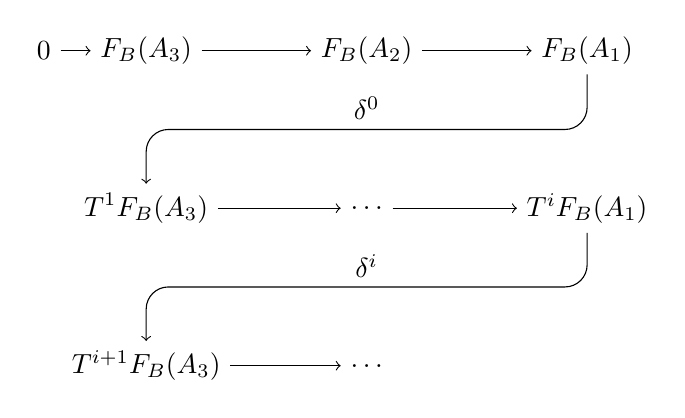
\begin{tikzpicture}[baseline=(current bounding box.center)]
        \node (zero) at (-1.3,2)
        {$0$}; \node (FA3) at (0,2)
        {$\mathscr{F}_B(A_3)$}; \node (FA2) at (2.8,2)
        {$\mathscr{F}_B(A_2)$}; \node (FA1) at (5.6,2)
        {$\mathscr{F}_B(A_1)$}; \node (T1A3) at (0,0)
        {$\categ{T}^1\mathscr{F}_B(A_3)$}; \node (dots1) at (2.8,0)
        {$\dots$}; \node (TiA1) at (5.6,0)
        {$\categ{T}^i\mathscr{F}_B(A_1)$}; \node (Ti1A3) at (0,-2)
        {$\categ{T}^{i+1}\mathscr{F}_B(A_3)$}; \node (dots2) at
        (2.8,-2)
        {$\dots$}; \draw[->] (zero) -- (FA3); \draw[->] (FA3) --
        (FA2); \draw[->] (FA2) -- (FA1); \draw[->] (T1A3) -- (dots1);
        \draw[->] (dots1) -- (TiA1); \draw[->] (Ti1A3) -- (dots2);
        \draw[->, rounded corners=8pt] (FA1.south) -- (5.6,1) --
        node[above]
        {$\delta^0$} (0,1) -- (T1A3.north); \draw[->, rounded
        corners=8pt] (TiA1.south) -- (5.6,-1) -- node[above]
        {$\delta^i$} (0,-1) -- (Ti1A3.north);
      \end{tikzpicture}
    \]
  \item Prove that the $\categ{T}^i\mathscr{F}_B$ form a
    $\delta$-functor, in the sense of Exercise~\ref{exer:homol:7.13}.
  \item Prove that if $E$ is an $\mathscr{F}$-exact object of
    $\categ{A}$, then $\categ{T}^i\mathscr{F}_B(E) = 0$ for $i > 0$,
    and deduce that the $\categ{T}^i\mathscr{F}_B$ form a
    \emph{universal} $\delta$-functor.
  \item Let
    $E^\bullet : \dots \to E^{-2} \to E^{-1} \to E^0 \to A \to 0$ be
    an $\mathscr{F}$-exact resolution of $A$. Then
    $\categ{T}^i\mathscr{F}_B \cong H^i(\mathscr{F}_B(E^\bullet))$.
    (Hint: Mimic the proof of Theorem~\ref{thm:homol:8.3}.)
  \end{itemize}
  The upshot is that the interplay of the two functors $\mathscr{F}^A$
  and $\mathscr{F}_B$ allows us to define $\categ{T}^i\mathscr{F}_B$
  as if it were a right-derived functor, using $\mathscr{F}$-exact
  objects in place of projectives. This gives a universal
  $\delta$-functor, which agrees with the standard right-derived
  functor when $\categ{A}$ has enough projectives (by
  Exercise~\ref{exer:homol:7.15} and the uniqueness of universal
  $\delta$-functors). [\S{}\ref{subsec:homol:resolution-by-acyclic-objects}]
\end{exer}

\section{Further topics}
\label{sec:homol:further-topics}

This last section touches upon issues that arise naturally in the
context of this chapter and for which a (much) more extensive
treatment would be needed. This will hopefully whet the reader's
appetite for more and encourage further study of homological algebra
beyond the basics covered here. I will be somewhat detailed in
\S{}9.3, illustrating the spectral sequence associated to a double
complex, since this can be done reasonably quickly (but delving into
any other application of spectral sequences would simply take us too
far). For the other themes in this section (derived and triangulated
categories) I will really do no more than a little propaganda.

\subsection{Derived categories}
\label{subsec:homol:derived-categories}
Derived categories made their appearance in \S{}4.2 and have since
served as a guiding concept motivating the natural development of the
subject, but we have stopped short of constructing them in
general. The closest we have come to a concrete description of the
derived category is in the `poor man's version' of \S{}6.3, which
should actually be labeled the `rich man's version', since it relies
on the fortunate presence of enough projectives/injectives. Also, the
versions $\categ{D}^-(\categ{A})$, $\categ{D}^+(\categ{A})$ considered
there are necessarily \emph{bounded}, as they rely on bounded
resolutions of objects and complexes in $\categ{A}$.  Derived
categories may be defined without such restrictions. For an abelian
category $\categ{A}$, the objects of $\categ{D}(\categ{A})$ are taken
to be the same as in $\categ{C}(\categ{A})$, that is, cochain
complexes; boundedness conditions may be included here, if desired. As
for morphisms, remember that the whole point of the derived category
is to `invert quasi-isomorphisms'; the most direct way to do this is
essentially the same as the process that allows us to `invert all
nonzero elements of an integral domain', leading to the construction
of the field of fractions (see \ref{subsec:irred:the-field-of-fractions-of-an-integral-domain}). This process, in a more
general version dealing with inverting `multiplicative subsets' of a
ring, is called \emph{localization} (\Cref{exer:irred:4.7}). Categories may
be localized as well. For example, the homotopic category
$\categ{K}(\categ{A})$ may be viewed as the localization of
$\categ{C}(\categ{A})$ with respect to homotopy equivalences: these
become isomorphisms in $\categ{K}(\categ{A})$.  Localizing
$\categ{K}(\categ{A})$ with respect to homotopy classes of
quasi-isomorphisms yields $\categ{D}(\categ{A})$.  In necessarily
oversimplified terms, suppose you want to make a class of morphisms of
a category $\categ{C}$ invertible. In the new category, any `roof'
diagram
\[\begin{tikzcd}
    & Z \arrow[dl,"\alpha"'] \arrow[dr,"\beta"] & \\
    A \arrow[rr,dashed] & & B
  \end{tikzcd}\] with $\alpha$ in that class will determine a morphism
$\beta \circ \alpha^{-1} : A \to B$; that is, the dashed arrow will
have to exist as a morphism in the new category. These are the analogs
of the `fractions' in the field of fractions; the localization of
$\categ{C}$ may be defined by taking the same objects as in
$\categ{C}$ and setting morphisms in the new category to be
compositions of `roofs', up to a suitable equivalence relation. For
example, all roofs
\[\begin{tikzcd}
    & Z \arrow[dl,"\alpha"'] \arrow[dr,"\alpha"] & \\
    A & & A
  \end{tikzcd}\] with $\alpha$ in the chosen class should be
identified to one another and to $\id_A$ in the
localized category; the roof
\[\begin{tikzcd}
    & Z \arrow[dl,"\alpha"'] \arrow[dr,"\id_Z"] & \\
    A & & Z
  \end{tikzcd}\] will work as the inverse of $\alpha$ in the
localization.

As the reader can imagine, working out the construction in earnest
requires dealing with nontrivial technical issues. These are more
manageable when the class of morphisms to be inverted is `localizing'
(for example, the composition of two such morphisms should also be a
morphism in the class); for example, this condition allows us to
represent the composition of two roofs as a roof. To mention one
set-theoretic difficulty, one should make sure that morphisms
$A \to B$ in the localization still form a \emph{set}, even if the
roofs connecting $A$ to $B$ may a priori form a proper \emph{class}.
With all these caveats in mind, the localization process can be
carried out on $\categ{K}(\categ{A})$ with respect to
quasi-isomorphisms and does produce a category $\categ{D}(\categ{A})$
satisfying the universal property for derived categories described in
\S{}4.2. If $\categ{A}$ has (for example) enough projectives, then the
bounded version $\categ{D}^-(\categ{A})$ is equivalent to the homotopy
category $\categ{K}^-(\categ{P})$ of complexes of projectives, as I
have endeavored to justify in \S{}6.3. The latter should be viewed as
a convenient way to `compute' the former in favorable circumstances.
Summarizing, a morphism $L^\bullet \to M^\bullet$ in the derived
category $\categ{D}(\categ{A})$ of an abelian category $\categ{A}$ can
be represented as a roof diagram
\[\begin{tikzcd}
    & N^\bullet \arrow[dl,"\text{quasi-isomorphism}"'] \arrow[dr] & \\
    L^\bullet & & M^\bullet
  \end{tikzcd}\] of (homotopy classes of) morphisms of cochain
complexes, modulo a suitable equivalence relation. Note that the
construction is applied to $\categ{K}(\categ{A})$, rather than the
simpler-minded $\categ{C}(\categ{A})$: for one thing, one might as
well start from $\categ{K}(\categ{A})$, since the functor
$\categ{C}(\categ{A}) \to \categ{D}(\categ{A})$ will have to factor
through the homotopic category (Proposition~\ref{prop:homol:5.4}). In
any case it just so happens that, unfortunately, quasi-isomorphisms do
not form a localizing class of morphisms in $\categ{C}(\categ{A})$,
while their homotopy classes \emph{are} localizing in
$\categ{K}(\categ{A})$. So it goes.  Once we believe that this
prescription does define a category---for example, that the
composition of two roofs can be represented by a roof and that this
composition is associative---then it is essentially clear that
$\categ{D}(\categ{A})$ satisfies the universal property specified in
\S{}4.2. However, the real benefits of introducing the derived
category lie deeper, for example in its structure as a
\emph{triangulated category}. A brief discussion of this concept
follows.

The reader should check that the composition of two roofs is indeed a
roof (Exercise~\ref{exer:homol:9.2}); this may be easier after
acquiring a little familiarity with distinguished triangles. Also,
note that the diagram in Exercise~\ref{exer:homol:9.2} does not
commute in $\categ{C}(\categ{A})$, but it does in
$\categ{K}(\categ{A})$. This is an indication that it would be
problematic to go `directly' from $\categ{C}(\categ{A})$ to
$\categ{D}(\categ{A})$.

\subsection{Triangulated categories}
\label{subsec:homol:triangulated-categories}
One reason for not treating derived categories to any real extent in
this book is that to do so would require us to define precisely the
notion of \emph{triangulated category}. The same applies in fact to
homotopic categories of complexes. I have pointed out in \S{}5.2 that
these categories should not be expected to be (and indeed are not)
\emph{abelian}, but they preserve enough structure to make sense of,
for example, long exact cohomology sequences. The fact that derived
functors ended up having long exact sequences associated to them
(\S{}7.4) bears witness to this fact.  The essential ingredients of a
triangulated (additive) category are a `translation' functor, which in
the case of $\categ{K}(\categ{A})$ or $\categ{D}(\categ{A})$ is
realized as the shift functor $L^\bullet \mapsto L[1]^\bullet$; and a
class of diagrams
\[
  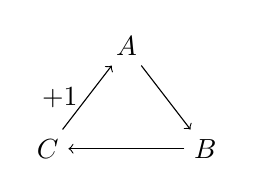
\begin{tikzpicture}[baseline=(current bounding box.center)]
    \node (A) at (1,1.3) {$A$}; \node (C) at (0,0)
    {$C$}; \node (B) at (2,0)
    {$B$}; \draw[->] (A) -- (B); \draw[->] (B) -- (C); \draw[->] (C)
    -- (A) node[midway, left] {$+1$};
  \end{tikzpicture}
\]
where the morphism labeled `$+1$' acts as $C \to A[1]$; these diagrams
are called \emph{distinguished triangles}. A common alternative
notation is
\[
  A \longrightarrow B \longrightarrow C \xrightarrow{+1}.
\]

Distinguished triangles are required to satisfy several axioms.  Among
them,
\[
  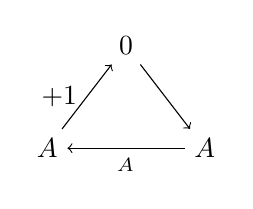
\begin{tikzpicture}[baseline=(current bounding box.center)]
    \node (T) at (1,1.3) {$0$}; \node (C) at (0,0)
    {$A$}; \node (B) at (2,0)
    {$A$}; \draw[->] (T) -- (B); \draw[->] (B) -- (C) node[midway,
    below]
    {$\id_A$}; \draw[->] (C) -- (T) node[midway, left]
    {$+1$};
  \end{tikzpicture}
\]
is required to be distinguished for every $A$; every morphism
$\alpha : A \to B$ must be a side of a distinguished triangle;
triangles isomorphic to a distinguished triangle (in the evident
sense) must be distinguished; and distinguished triangles can be
`rotated':
\[
  \begin{tikzpicture}[baseline=(current bounding box.center)]
    \node (A) at (1,1.3) {$A$}; \node (C) at (0,0)
    {$C$}; \node (B) at (2,0)
    {$B$}; \draw[->] (A) -- (B) node[midway, right]
    {$\alpha$}; \draw[->] (B) -- (C) node[midway, below]
    {$\beta$}; \draw[->] (C) -- (A) node[midway, left]
    {$\substack{+1\\\gamma}$};
  \end{tikzpicture}
\]
is distinguished if and only if
\[
  \begin{tikzpicture}[baseline=(current bounding box.center)]
    \node (B) at (1,1.3) {$B$}; \node (A) at (0,0)
    {$A[1]$}; \node (C) at (2,0)
    {$C$}; \draw[->] (B) -- (C) node[midway, right]
    {$\beta$}; \draw[->] (C) -- (A) node[midway, below]
    {$\gamma$}; \draw[->] (A) -- (B) node[midway, left]
    {$\substack{+1\\-\alpha}$};
  \end{tikzpicture}
\]
is distinguished. There is more, including an infamous
\emph{octahedral axiom} (so named since a popular way to state it
invokes an octahedral diagram). The reader will have no difficulties
locating this information in the literature.  The category
$\categ{K}(\categ{A})$ is triangulated: the translation functor is the
basic shift of a complex, and distinguished triangles are those
isomorphic to
\[
  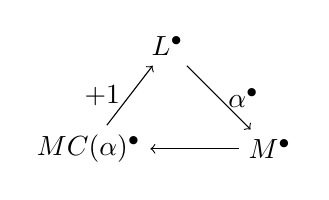
\begin{tikzpicture}[baseline=(current bounding box.center)]
    \node (L) at (1,1.3)
    {$L^\bullet$}; \node (MC) at (0,0)
    {$MC(\alpha)^\bullet$}; \node (M) at (2.3,0)
    {$M^\bullet$}; \draw[->] (L) -- (M) node[midway, right]
    {$\alpha^\bullet$}; \draw[->] (M) -- (MC); \draw[->] (MC) -- (L)
    node[midway, left] {$+1$};
  \end{tikzpicture}
\]
That is, the `third vertex' of a triangle with an assigned side
$\alpha^\bullet : L^\bullet \to M^\bullet$ is the mapping cone of
$\alpha^\bullet$, and the unlabeled sides are the natural cochain
morphisms $M^\bullet \to MC(\alpha)^\bullet$,
$MC(\alpha)^\bullet \to L[1]^\bullet$ studied in \S{}4.1.

It would be problematic to make the same choice in
$\categ{C}(\categ{A})$, since while
\[
  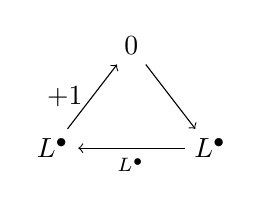
\begin{tikzpicture}[baseline=(current bounding box.center)]
    \node (T) at (1,1.3) {$0$}; \node (Z) at (0,0)
    {$L^\bullet$}; \node (B) at (2,0)
    {$L^\bullet$}; \draw[->] (T) -- (B); \draw[->] (B) -- (Z)
    node[midway, below]
    {$\id_{L^\bullet}$}; \draw[->] (Z) -- (T)
    node[midway, left] {$+1$};
  \end{tikzpicture}
\]
would be distinguished as needed, since $L^\bullet$ is the mapping
cone of the zero-morphism $0 \to L^\bullet$, the rotation of this
triangle, i.e.,
\[
  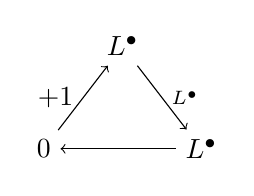
\begin{tikzpicture}[baseline=(current bounding box.center)]
    \node (L) at (1,1.3) {$L^\bullet$}; \node (Z) at (0,0)
    {$0$}; \node (B) at (2,0)
    {$L^\bullet$}; \draw[->] (L) -- (B) node[midway, right]
    {$\id_{L^\bullet}$}; \draw[->] (B) -- (Z); \draw[->]
    (Z) -- (L) node[midway, left] {$+1$};
  \end{tikzpicture}
\]
would not seem to be, since the mapping cone of the identity is not
$0$. But the mapping cone of the identity is \emph{homotopically
  equivalent} to $0$ (Exercise~\ref{exer:homol:9.3}), so the rotated
triangle is indeed distinguished in $\categ{K}(\categ{A})$, as it
should be, according to the axioms. More generally, it is easy to see
(Exercise~\ref{exer:homol:9.4}) that if
$\alpha^\bullet : L^\bullet \to M^\bullet$ is a cochain morphism, so
that we have a distinguished triangle,
\[
  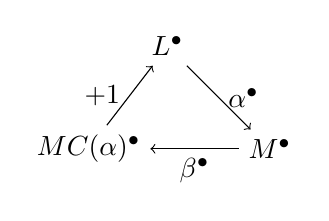
\begin{tikzpicture}[baseline=(current bounding box.center)]
    \node (L) at (1,1.3)
    {$L^\bullet$}; \node (MC) at (0,0)
    {$MC(\alpha)^\bullet$}; \node (M) at (2.3,0)
    {$M^\bullet$}; \draw[->] (L) -- (M) node[midway, right]
    {$\alpha^\bullet$}; \draw[->] (M) -- (MC) node[midway, below]
    {$\beta^\bullet$}; \draw[->] (MC) -- (L) node[midway, left]
    {$+1$};
  \end{tikzpicture}
\]
then the mapping cone of $\beta^\bullet$ is in fact homotopy
equivalent to $L[1]^\bullet$; the rotation
\[
  (*) \qquad
  \begin{tikzpicture}[baseline=(current bounding box.center)]
    \node (M) at (1,1.3)
    {$M^\bullet$}; \node (L1) at (0,0)
    {$L[1]^\bullet$}; \node (MC) at (2.3,0)
    {$MC(\alpha)^\bullet$}; \draw[->] (M) -- (MC) node[midway, right]
    {$\beta^\bullet$}; \draw[->] (MC) -- (L1); \draw[->] (L1) -- (M)
    node[midway, left] {$\substack{+1\\-\alpha^\bullet}$};
  \end{tikzpicture}
\]
is distinguished as required, as the reader should check.
\emph{Applying the cohomology functor to a distinguished triangle in
  $\categ{K}(\categ{A})$ yields an exact triangle}: indeed, as we have
just seen, we may assume that the triangle is $(*)$ (up to isomorphism
in $\categ{K}(\categ{A})$), and taking cohomology gives the exact
triangle
\[
  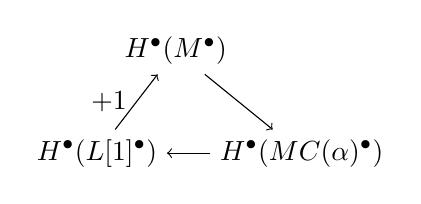
\begin{tikzpicture}[baseline=(current bounding box.center)]
    \node (M) at (1,1.3)
    {$H^\bullet(M^\bullet)$}; \node (L1) at (0,0)
    {$H^\bullet(L[1]^\bullet)$}; \node (MC) at (2.6,0)
    {$H^\bullet(MC(\alpha)^\bullet)$}; \draw[->] (M) -- (MC);
    \draw[->] (MC) -- (L1); \draw[->] (L1) -- (M) node[midway, left]
    {$+1$};
  \end{tikzpicture}
\]
obtained in Proposition~\ref{homol:4.1}. In general, a
\emph{cohomological functor} on a triangulated category is an additive
functor to an abelian category, mapping distinguished triangles to
exact triangles and hence inducing long exact sequences. Thus,
cohomology is a cohomological functor on $\categ{K}(\categ{A})$; this
will not surprise the reader. The functors $\Hom(A,\_)$
and $\Hom(\_,A)$ (to $\categ{Ab}$) are cohomological
functors on every triangulated category, for every object $A$.

The derived category $\categ{D}(\categ{A})$ and its bounded versions
are triangulated categories, with distinguished triangles described as
above---that is, isomorphic (in $\categ{D}(\categ{A})$) to the basic
triangles determined by mapping cones. The natural functor
$\categ{K}(\categ{A}) \to \categ{D}(\categ{A})$ is a functor of
triangulated categories, in the sense that it preserves the
translation functor and it sends distinguished triangles to
distinguished triangles.

Isomorphism in the derived category is a less stringent notion than in
the homotopic category, so there are `more' distinguished triangles in
$\categ{D}(\categ{A})$ than in $\categ{K}(\categ{A})$.  For example,
if
\[
  0 \longrightarrow L^\bullet \xrightarrow{\alpha^\bullet} M^\bullet
  \xrightarrow{\beta^\bullet} N^\bullet \longrightarrow 0
\]
is a short exact sequence, as above, there is in general no
distinguished triangle
\[
  \begin{tikzpicture}[baseline=(current bounding box.center)]
    \node (L) at (1,1.3)
    {$L^\bullet$}; \node (N) at (0,0)
    {$N^\bullet$}; \node (M) at (2,0)
    {$M^\bullet$}; \draw[->] (L) -- (M) node[midway, right]
    {$\alpha^\bullet$}; \draw[->] (M) -- (N) node[midway, below]
    {$\beta^\bullet$}; \draw[->] (N) -- (L) node[midway, left]
    {$\substack{+1\\\gamma^\bullet}$};
  \end{tikzpicture}
\]
in $\categ{K}(\categ{A})$ (for any choice of $\gamma^\bullet$):
indeed, $N^\bullet$ need not\footnote{Why? Construct an example
  showing this.} be homotopically equivalent to $MC(\alpha)^\bullet$.
But such triangles \emph{do} exist in $\categ{D}(\categ{A})$!  In
fact, we are now well-equipped to make (better) sense of the
mysterious remarks at the end of \S{}3.4. The `special triangles'
\[
  \begin{tikzpicture}[baseline=(current bounding box.center)]
    \node (L) at (1,1.3)
    {$L^\bullet$}; \node (N) at (0,0)
    {$N^\bullet$}; \node (M) at (2,0)
    {$M^\bullet$}; \draw[->] (L) -- (M); \draw[->] (M) -- (N);
    \draw[->] (N) -- (L) node[midway, left] {$\substack{+1\\0}$};
  \end{tikzpicture}
\]
arising as in \S{}3.4 from a short exact sequence
\[
  0 \longrightarrow L^\bullet \xrightarrow{\alpha^\bullet} M^\bullet
  \xrightarrow{\beta^\bullet} N^\bullet \longrightarrow 0
\]
are not distinguished in $\categ{K}(\categ{A})$, and in general no
replacement for the zero-morphism will fix this problem. On the other
hand, the reader can now verify (Exercise~\ref{exer:homol:9.5}) that
there is a quasi-isomorphism $MC(\alpha)^\bullet \to N^\bullet$: this
can be shown by computing explicitly another mapping cone and applying
Corollary~\ref{homol:4.2}. Thus, in the derived category the standard
distinguished triangle
\[
  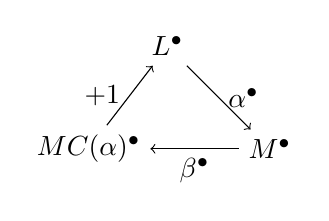
\begin{tikzpicture}[baseline=(current bounding box.center)]
    \node (L) at (1,1.3)
    {$L^\bullet$}; \node (MC) at (0,0)
    {$MC(\alpha)^\bullet$}; \node (M) at (2.3,0)
    {$M^\bullet$}; \draw[->] (L) -- (M) node[midway, right]
    {$\alpha^\bullet$}; \draw[->] (M) -- (MC) node[midway, below]
    {$\beta^\bullet$}; \draw[->] (MC) -- (L) node[midway, left]
    {$+1$};
  \end{tikzpicture}
\]
is isomorphic to a triangle
\[
  \begin{tikzpicture}[baseline=(current bounding box.center)]
    \node (L) at (1,1.3)
    {$L^\bullet$}; \node (N) at (0,0)
    {$N^\bullet$}; \node (M) at (2,0)
    {$M^\bullet$}; \draw[->] (L) -- (M) node[midway, right]
    {$\alpha^\bullet$}; \draw[->] (M) -- (N) node[midway, below]
    {$\beta^\bullet$}; \draw[->] (N) -- (L) node[midway, left]
    {$\substack{+1\\\gamma^\bullet}$};
  \end{tikzpicture}
\]
which is therefore distinguished in $\categ{D}(\categ{A})$ (cf.\
Exercise~\ref{exer:homol:9.6}). Applying the cohomology functor to
this triangle directly gives the exact triangle
\[
  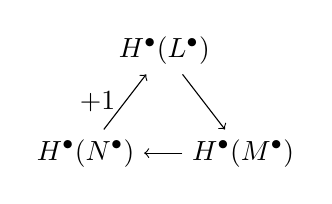
\begin{tikzpicture}[baseline=(current bounding box.center)]
    \node (L) at (1,1.3)
    {$H^\bullet(L^\bullet)$}; \node (N) at (0,0)
    {$H^\bullet(N^\bullet)$}; \node (M) at (2,0)
    {$H^\bullet(M^\bullet)$}; \draw[->] (L) -- (M); \draw[->] (M) --
    (N); \draw[->] (N) -- (L) node[midway, left] {$+1$};
  \end{tikzpicture}
\]
expressing the long exact cohomology sequence as in \S{}3.4, without
having to single out the $+1$ morphism for special consideration. In
retrospect, the zero-morphism I insisted on using when folding
`special' triangles in \S{}3.4 turns out to be an artifact: placing
the triangle in the derived category shows that there is a more
informed choice for this morphism. This choice is not available in
$\categ{C}(\categ{A})$ and is not even in $\categ{K}(\categ{A})$, but
it \emph{is} available in $\categ{D}(\categ{A})$ and leads
transparently to the long exact sequence in cohomology.

If $\mathscr{F} : \categ{A} \to \categ{B}$ is a functor between
abelian categories, the induced functor
$\categ{K}(\mathscr{F}) : \categ{K}(\categ{A}) \to
\categ{K}(\categ{B})$ is a functor of triangulated categories, and so
are the bounded variations
$\categ{K}^\pm(\mathscr{F}) : \categ{K}^\pm(\categ{A}) \to
\categ{K}^\pm(\categ{B})$. The derived functors
$\categ{L}\mathscr{F}, \categ{R}\mathscr{F} : \categ{D}^\pm(\categ{A})
\to \categ{D}^\pm(\categ{B})$ encountered in \S{}7.2 are also functors
of triangulated categories.  This fact is responsible for the good
properties of derived functors, such as the long exact sequences
studied in \S{}7.4.

\subsection{Spectral sequences}
\label{subsec:homol:spectral-sequences}
I mentioned in \S{}8.3 that `spectral sequences' may be used to
compute the cohomology of a double complex. There unfortunately does
not seem to be an easy entry point in the subject of spectral
sequences, which is marred by intrinsic notational complexity. I will
limit myself to a very scant description of the concept and some
information linking it back to \S{}8.4. My motivation is that, in the
literature, references to results such as \Cref{thm:homol:8.12} are often
replaced by sentences such as `by an immediate spectral sequence
argument\dots', and I should try to explain to the reader what this
means.

Given that we were thinking about triangles a moment ago, the
following construction may be helpful in appreciating the notion of
spectral sequence. Let
\[
  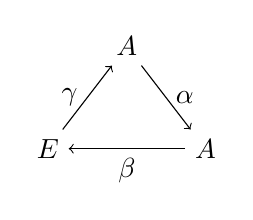
\begin{tikzpicture}[baseline=(current bounding box.center)]
    \node (A) at (1,1.3) {$A$}; \node (E) at (0,0)
    {$E$}; \node (A2) at (2,0)
    {$A$}; \draw[->] (A) -- (A2) node[midway, right]
    {$\alpha$}; \draw[->] (A2) -- (E) node[midway, below]
    {$\beta$}; \draw[->] (E) -- (A) node[midway, left] {$\gamma$};
  \end{tikzpicture}
\]
be an exact triangle\footnote{That is,
  $\image\alpha = \ker\beta$,
  $\image\beta = \ker\gamma$, and
  $\image\gamma = \ker\alpha$.} in an abelian category; I
am placing no assumption on the `degree' of $\gamma$ (and indeed, I am
not assuming we have defined a translation functor).

Let $d : E \to E$ be the composition $\beta \circ \gamma$; since
$\gamma \circ \beta = 0$, we have
\[
  d \circ d = \beta \circ (\gamma \circ \beta) \circ \gamma = 0.
\]
Thus we can take the homology of $E$ with respect to $d$ and define
\[
  E' := \frac{\ker d}{\image d}.
\]
Further, we can let $A' := \image\alpha$ and let
\begin{itemize}
\item $\alpha' : A' \to A'$ be the restriction of $\alpha$ to $A'$;
\item $\beta' : A' \to E'$ be defined by
  $\beta'(\alpha(a)) := [\beta(a)]$;
\item $\gamma' : E' \to A'$ be defined by $\gamma'([e]) := \gamma(e)$,
\end{itemize}
where $[e]$ denotes the class of $e \in E$ in $E'$. (Since
$\beta \circ \gamma(e) = d(e) = 0$,
$\gamma(e) \in \ker\beta = \image\alpha = A'$.) All needed
verifications (such as the independence on the representative $e$ of
$[e]$ in the third prescription) are straightforward, from the
exactness of the given triangle.

\begin{fact}{\Cref{fact:homol:9.1}}{fact:homol:9.1}
  The new triangle
  \[
    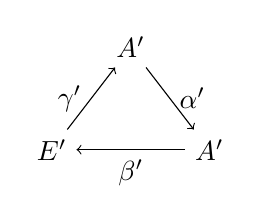
\begin{tikzpicture}[baseline=(current bounding box.center)]
      \node (A) at (1,1.3) {$A'$}; \node (E) at (0,0)
      {$E'$}; \node (A2) at (2,0)
      {$A'$}; \draw[->] (A) -- (A2) node[midway, right]
      {$\alpha'$}; \draw[->] (A2) -- (E) node[midway, below]
      {$\beta'$}; \draw[->] (E) -- (A) node[midway, left] {$\gamma'$};
    \end{tikzpicture}
  \]
  is again exact.
\end{fact}

The reader will have no difficulty proving this statement
(Exercise~\ref{exer:homol:9.7}).

The datum of an exact triangle as above is called an \emph{exact
  couple}, which I find confusing since a triangle has three vertices
(but it is true that only two objects are involved here); the new
exact triangle (couple) obtained in Claim~\ref{fact:homol:9.1} is the
\emph{derived couple}, which I find even more confusing since there is
no derived category or functor in sight. Exact couples arose in
topology (they are due to W. Massey), and the terminology reflects
their origin.

Of course we can turn the crank at will and get derived couple after
derived couple: let $A_1 = A$, $E_1 = E$, etc., and inductively define
$A_{i+1} := A'_i$, $E_{i+1} := E'_i$, etc. For example, $\beta_{i+1}$
is obtained by `rewinding' the morphism $\alpha$ a total of $i$ times
and then applying the original morphism $\beta$: we can do this since
$A_{i+1}$ is the image of $\alpha^i$.

Thus, one exact triangle produces a whole sequence of triangles and in
particular a sequence of objects $E_i$, each endowed with a
differential $d_i$, such that
$E_{i+1} = \ker d_i / \image d_i$.

\begin{defn}{}{defn:homol:9.2}
  A \emph{spectral sequence} $\{(E_i, d_i)\}_{i=1,2,\dots}$ is a
  sequence of objects $E_i$ and morphisms $d_i : E_i \to E_i$ in an
  abelian category, such that $d_i \circ d_i = 0$ and
  $E_{i+1} \cong \ker d_i / \image d_i$.
\end{defn}

Thus, exact couples are a way to produce spectral sequences. There is
a sense in which we can turn the crank `infinitely many times'; in
fact, this can be done with any spectral sequence. To see this, let
\[
  Z_1 = E_1, \quad B_1 = 0,
\]
so that $E_1 \cong Z_1/B_1$; inductively, assume we have defined
$Z_i \subseteq Z_1$, $B_i \subseteq Z_i$ so that $E_i \cong Z_i/B_i$,
and let $\overline{Z}_{i+1} = \ker d_i$,
$\overline{B}_{i+1} = \image d_i$; define $Z_{i+1}$,
$B_{i+1}$ as the corresponding subobjects of $Z_i$. Then
\[
  E_{i+1} \cong \frac{\overline{Z}_{i+1}}{\overline{B}_{i+1}} \cong
  \frac{Z_{i+1}}{B_{i+1}},
\]
realizing $E_{i+1}$ as a \emph{subquotient}\footnote{That is, as a
  quotient of a subobject.} of $E_1$, and
\[
  B_1 \subseteq \dots \subseteq B_i \subseteq B_{i+1} \subseteq \dots
  \subseteq Z_{i+1} \subseteq Z_i \subseteq \dots \subseteq Z_1.
\]
Define\footnote{Here I am implicitly working in a category
  $R\text{-}\categ{Mod}$ of modules over a ring, containing the given
  abelian category $\categ{A}$ (invoking the Freyd--Mitchell theorem,
  Theorem~\ref{homol:2.9}). The infinite unions and intersections used
  here make sense in $R\text{-}\categ{Mod}$; the limits and the
  corresponding $E_\infty$ are therefore defined as objects in
  $R\text{-}\categ{Mod}$ and in general not as objects of $\categ{A}$.
  But if, e.g., the sequence collapses at $E_r$, then
  $B_\infty = B_r$, $Z_\infty = Z_r$, and $E_\infty$ exists in
  $\categ{A}$. In practice, this difficulty will play no role in the
  considerations that follow.}
\[
  B_\infty := \bigcup_i B_i, \quad Z_\infty := \bigcap_i Z_i, \quad
  E_\infty := \frac{Z_\infty}{B_\infty}.
\]
This `ultimate' subquotient $E_\infty$ is the \emph{limit} of the
spectral sequence; it is common to say that the spectral sequence
$E_r$ \emph{abuts} to $E_\infty$. By definition, if
$d_r = d_{r+1} = \dots = 0$, then $Z_\infty = Z_r$ and
$B_\infty = B_r$, so that $E_\infty \cong E_r$; in this case we say
that the sequence \emph{collapses} at $E_r$.

The reader will verify (Exercise~\ref{exer:homol:9.8}) that if the
spectral sequence arises from an exact couple, as above, then
\[
  Z_\infty = \bigcap_r \gamma^{-1}(\image \alpha^r), \quad
  B_\infty = \bigcup_r \beta(\ker \alpha^r),
\]
so the limit $E_\infty$ has a concrete realization in this case.

Typically, a spectral sequence is as interesting as its limit,
especially if some fortunate circumstance causes its collapse very
soon; it is not too uncommon to have situations in which
$E_\infty = E_2$. If all goes well, this translates into a useful
relation between the given `input' $E_1$ and the interesting `output'
$E_\infty$.  \emph{Where is my double complex?} I promised that
spectral sequences could be used to `compute' the cohomology of the
total complex of a double complex. We will now see how a double
complex gives rise to an exact couple and hence to a spectral
sequence. This is a particular case of a useful mechanism producing an
exact sequence from a filtration.

A `descending filtration' of $M$ consists of a sequence of subobjects:
\[
  M \supseteq \dots \supseteq M_m \supseteq M_{m+1} \supseteq \dots.
\]
For example, the series of subgroups of a group $G$ considered in
\ref{subsec:groups2:the-jordan-h-older-theorem} are filtrations of $G$. If $M$ is an object of an abelian
category, a filtration as above determines an associated \emph{graded
  object}
\[
  \operatorname{gr}(M) := \bigoplus_m \operatorname{gr}(M)_m, \quad
  \operatorname{gr}(M)_m := \frac{M_m}{M_{m+1}};
\]
I will assume this is an object of the same category for simplicity,
although this is not necessarily the case (abelian categories are not
necessarily closed under infinite direct sums); since only finitely
many objects will be involved in any specific computation, this plays
no role.

Start with a double complex $M^{\bullet,\bullet}$; I will assume that
$M^{i,j} = 0$ for $i < 0$, $j < 0$:
\[\begin{tikzcd}
    \vdots & \vdots & \vdots & \vdots & \\
    M^{0,2} \arrow[r,"d_h"] \arrow[u,"\delta_v"] & M^{1,2} \arrow[r,"d_h"] \arrow[u,"\delta_v"] & M^{2,2} \arrow[r,"d_h"] \arrow[u,"\delta_v"] & M^{3,2} \arrow[r,"d_h"] \arrow[u,"\delta_v"] & \cdots \\
    M^{0,1} \arrow[r,"d_h"] \arrow[u,"\delta_v"] & M^{1,1} \arrow[r,"d_h"] \arrow[u,"\delta_v"] & M^{2,1} \arrow[r,"d_h"] \arrow[u,"\delta_v"] & M^{3,1} \arrow[r,"d_h"] \arrow[u,"\delta_v"] & \cdots \\
    M^{0,0} \arrow[r,"d_h"] \arrow[u,"\delta_v"] & M^{1,0}
    \arrow[r,"d_h"] \arrow[u,"\delta_v"] & M^{2,0} \arrow[r,"d_h"]
    \arrow[u,"\delta_v"] & M^{3,0} \arrow[r,"d_h"]
    \arrow[u,"\delta_v"] & \cdots
  \end{tikzcd}\] As always, zero-objects to the left and below the
given part of the diagram are implicit; we are assuming (as in
\Cref{defn:homol:8.5}) that the diagram anticommutes, so that the
differential of the total complex $TC(M)^\bullet$ is simply
$d_h + \delta_v$. Analogous results can be obtained if $M^{i,j} = 0$
for $i > 0$, $j > 0$ and in fact under more relaxed hypotheses; such
considerations are left to the reader.

Let $T^\bullet = TC(M)^\bullet$ denote the total complex: therefore,
$T^k = \bigoplus_{i+j=k} M^{i,j}$. This complex admits (at least) two
filtrations: a \emph{horizontal} filtration and a \emph{vertical}
filtration. I will focus on the vertical one, and again it is
understood that a parallel discussion would hold for the horizontal
one. The vertical filtration $T^\bullet_m$ is defined by chopping off
the terms to the left of a vertical bar $i = m$ in the diagram
\[\begin{tikzcd}
    & \vdots & \vdots & \\
    \cdots & M^{m,2} \arrow[r,"d_h"] \arrow[u,"\delta_v"] & M^{m+1,2} \arrow[r,"d_h"] \arrow[u,"\delta_v"] & \cdots \\
    \cdots & M^{m,1} \arrow[r,"d_h"] \arrow[u,"\delta_v"] & M^{m+1,1} \arrow[r,"d_h"] \arrow[u,"\delta_v"] & \cdots \\
    \cdots & M^{m,0} \arrow[r,"d_h"] \arrow[u,"\delta_v"] & M^{m+1,0}
    \arrow[r,"d_h"] \arrow[u,"\delta_v"] & \cdots
  \end{tikzcd}\] That is, we set
\[
  T_m^k := \bigoplus_{\substack{i+j=k\\i \ge m}} M^{i,j},
\]
still with differential $d_h + \delta_v$. I will denote the
corresponding graded object by $\operatorname{gr}^\bullet_v(T)$, to
record the fact that this arises from the vertical filtration. (The
$\bullet$ reminds us that this is still a complex.) Explicitly, the
term of `filtration degree' $m$ in $\operatorname{gr}^k_v(T)$ is
\[
  \operatorname{gr}^k_v(T)_m = T_m^k / T_{m+1}^k = \bigoplus_{i \ge m}
  M^{i,k-i} \Big/ \bigoplus_{i \ge m+1} M^{i,k-i} \cong M^{m,k-m}.
\]
The differential $d_h + \delta_v$ induces the differential $\delta_v$
on this graded piece, since $d_h$ is zero modulo the next piece of the
filtration. The modules on the original array can therefore be labeled
as follows:
% ..  ..  ..  ..  . O K K K K K . O K K K K K . O K K K K K . O F F F
% F F
\[\begin{tikzcd}[column sep=small]
    \vdots & \vdots & \vdots & \vdots & \\
    \operatorname{gr}^2_v(T)_0 \arrow[r,dashed] & \operatorname{gr}^3_v(T)_1 \arrow[r,dashed] & \operatorname{gr}^4_v(T)_2 \arrow[r,dashed] & \operatorname{gr}^5_v(T)_3 & \cdots \\
    \operatorname{gr}^1_v(T)_0 \arrow[u] \arrow[r,dashed] & \operatorname{gr}^2_v(T)_1 \arrow[u] \arrow[r,dashed] & \operatorname{gr}^3_v(T)_2 \arrow[u] \arrow[r,dashed] & \operatorname{gr}^4_v(T)_3 \arrow[u] & \cdots \\
    \operatorname{gr}^0_v(T)_0 \arrow[u] \arrow[r,dashed] &
    \operatorname{gr}^1_v(T)_1 \arrow[u] \arrow[r,dashed] &
    \operatorname{gr}^2_v(T)_2 \arrow[u] \arrow[r,dashed] &
    \operatorname{gr}^3_v(T)_3 \arrow[u] & \cdots
  \end{tikzcd}\] with dashes connecting pieces with the same degree in
$\operatorname{gr}^\bullet_v(T)$.

The filtration on $T^\bullet$ also determines a filtration on the
cohomology of $T^\bullet$: we can take $H^\bullet(T^\bullet)_m$ to be
the image in $H^\bullet(T^\bullet)$ of $H^\bullet(T_m^\bullet)$.
Thus, we also have a graded object
$\operatorname{gr}_v H^\bullet(T^\bullet)$. \emph{The relation between
  $H^\bullet(\operatorname{gr}_v^\bullet(T))$ and
  $\operatorname{gr}_v H^\bullet(T^\bullet)$ is subtle: this relation
  is what spectral sequences will help us understand.}

The monomorphisms $T_{m+1}^\bullet \subseteq T_m^\bullet$ define a
monomorphism $\bigoplus_m T_m^\bullet \to \bigoplus_m T_m^\bullet$, of
which $\operatorname{gr}_v^\bullet(T)$ is the cokernel: we have an
exact sequence
\[
  (\dagger) \qquad 0 \longrightarrow \bigoplus_m T_m^\bullet
  \longrightarrow \bigoplus_m T_m^\bullet \longrightarrow
  \operatorname{gr}_v^\bullet(T) \longrightarrow 0 \, .
\]
As we know since \S{}3.3, this determines an exact triangle (couple!)
\[
  \begin{tikzpicture}[baseline=(current bounding box.center)]
    \node (A) at (1,1.3) {$H^\bullet(\bigoplus_m
      T_m^\bullet)$}; \node (E) at (0,0)
    {$H^\bullet(\operatorname{gr}_v^\bullet(T))$}; \node (A2) at (3,0)
    {$H^\bullet(\bigoplus_m
      T_m^\bullet)$}; \draw[->] (A) -- (A2) node[midway, right]
    {$\alpha$}; \draw[->] (A2) -- (E) node[midway, below]
    {$\beta$}; \draw[->] (E) -- (A) node[midway, left]
    {$\substack{+1\\\gamma}$};
  \end{tikzpicture}
\]
Note that $\alpha$ decreases the filtration degree by $1$, leaving the
cohomology degree $k$ unchanged; $\beta$ leaves both unchanged; and
$\gamma$ increases both by $1$. This is particularly clear if one
draws a small slice of the sequence $(\dagger)$, sufficient to see the
connecting morphism in action on a piece of given filtration and
cohomology degrees:
\[\begin{tikzcd}
    0 \arrow[r] & T_{m+1}^{k+1} \arrow[r] & T_m^{k+1} \arrow[r] &
    \operatorname{gr}_v^{k+1}(T)_m \arrow[r] & 0 \\
    0 \arrow[r] & T_{m+1}^k \arrow[r] \arrow[u] & T_m^k \arrow[r]
    \arrow[u] & \operatorname{gr}_v^k(T)_m \arrow[r] \arrow[u]
    \arrow[from=2-4,to=1-2,dashed,"\gamma" description, bend left=15]
    & 0
  \end{tikzcd}\]

\begin{defn}{}{defn:homol:9.3}
  The \emph{spectral sequence of the double complex}
  $M^{\bullet,\bullet}$ (with respect to the vertical filtration) is
  the spectral sequence determined by this exact couple.
\end{defn}

I will denote this spectral sequence by ${}_vE$, with the absurdly
positioned index $v$ recording that ${}_vE$ arises from the
\emph{vertical} filtration. The horizontal filtration leads likewise
to a spectral sequence ${}_hE$.

All terms ${}_vE_r$ of the spectral sequence are subquotients of the
first one, ${}_vE_1 = H^\bullet(\operatorname{gr}_v^\bullet(T))$.

\begin{rem}{}{homol:9.4}
  The differential $d_r = \beta_r \circ \gamma_r$ acts by increasing
  the cohomological degree $k$ by $1$ and the filtration degree $m$ by
  $r$: indeed, $\gamma_r$ is simply
  % induced by \gamma , so it increases both k and m by 1 (as observed
  % above); \beta r is obtained by applying \beta
  after undoing $(r-1)$ times the effect of $\alpha$ (as pointed out
  after Claim~\ref{fact:homol:9.1}), so it does not change $k$ but
  increases $m$ by $(r-1)$.
\end{rem}

Interest in the sequence rests on the interpretation for its limit in
the statement that follows, which also summarizes the situation.

\begin{thm}{}{homol:9.5}
  Let $M^{\bullet,\bullet}$ be a double complex in an abelian
  category. Assume that $M^{i,j} = 0$ for $i < 0$, $j < 0$, and let
  $T^\bullet$ be the total complex of $M^{\bullet,\bullet}$. Then,
  with notation as above, there exists a spectral sequence
  $\{({}_vE_i, d_i)\}_i$ such that
  \[ {}_vE_1 \cong H^\bullet(\operatorname{gr}_v^\bullet(T)), \qquad
    {}_vE_\infty \cong \operatorname{gr}_v H^\bullet(T^\bullet).
  \]
  In other words, `turning the crank' moves the $\operatorname{gr}$
  from inside the cohomology to outside of it. The limit
  ${}_vE_\infty$ does not quite compute the cohomology of the total
  complex, as I glibly announced in \S{}8.3, but it computes the
  graded object determined by a filtration on the cohomology of the
  total complex, and this is good enough for many applications.
\end{thm}
% Proof. The limit v E \infty can be computed directly from the exact
% couple (Exer- cise 9.8), as a subquotient of v E 1 : it is the
% quotient Z\infty /B\infty , where
\begin{proof}
  The limit ${}_vE_\infty$ can be computed directly from the exact
  couple (Exercise~\ref{exer:homol:9.8}), as a subquotient of
  ${}_vE_1$: it is the quotient $Z_\infty/B_\infty$, where
  \[
    Z_\infty = \bigcap_r \gamma^{-1}(\image\alpha^r),
    \qquad B_\infty = \beta\Big(\bigcup_r \ker\alpha^r\Big).
  \]
  The computation is streamlined by focusing on a specific degree $k$
  for the cohomology and $m$ for the grading. The corresponding part
  in ${}_vE_1$ is $H^k(T_m^\bullet/T_{m+1}^\bullet)$, and $\alpha$
  acts as $H^k(T_m^\bullet) \to H^k(T_{m-1}^\bullet)$. Note that if
  $r \gg 0$, then
  \[
    H^k(T_{m+r}^\bullet) = 0, \qquad H^k(T_{m-r}^\bullet) =
    H^k(T^\bullet),
  \]
  under our boundedness hypothesis: indeed, $T_i^j = 0$ if $i > j$,
  and $T_i^\bullet = T^\bullet$ for $i \le 0$.

  By the first of these observations, the piece sent by $\alpha^r$ to
  $H^k(T_m^\bullet)$ is $0$ for $r \gg 0$, and it follows that
  $\bigcap_r \image\alpha^r = 0$. Therefore,
  \[
    Z_\infty = \ker\gamma = \image\beta.
  \]
  By the second observation, $\ker\alpha^r$ stabilizes to
  $\ker(H^k(T_m^\bullet) \to H^k(T^\bullet))$ for each $k$, hence
  \[
    B_\infty = \beta\Big(\bigoplus_m \ker(H^\bullet(T_m^\bullet) \to
    H^\bullet(T^\bullet))\Big).
  \]

  Denote by $\nu_m : H^\bullet(T_m^\bullet) \to H^\bullet(T^\bullet)$
  the morphisms induced in cohomology by the monomorphisms
  $T_m^\bullet \to T^\bullet$ and by $\nu = \bigoplus_m \nu_m$ their
  direct sum. We have morphisms
  \[
    H^\bullet(\operatorname{gr}_v^\bullet(T)) \xleftarrow{\ \beta\ }
    \bigoplus_m H^\bullet(T_m^\bullet) \xrightarrow{\ \nu\ }
    \bigoplus_m H^\bullet(T^\bullet),
  \]
  and we have obtained
  \[ {}_vE_\infty \cong \frac{\image\beta}{\beta(\ker\nu)}.
  \]

  By the innocent \Cref{exer:homol:2.12},
  \[
    \frac{\image\beta}{\beta(\ker\nu)} \cong
    \frac{\image\nu}{\nu(\ker\beta)};
  \]
  by the exactness of the original couple,
  \[
    \ker\beta = \image\alpha = \bigoplus_m
    \image(H^\bullet(T_{m+1}^\bullet) \to
    H^\bullet(T_m^\bullet)),
  \]
  hence
  \[
    \nu(\ker\beta) = \bigoplus_m \image\nu_{m+1}.
  \]
  Therefore
  \[ {}_vE_\infty \cong \bigoplus_m \frac{\image\nu_m}
    {\image\nu_{m+1}} =
    \operatorname{gr}_v(H^\bullet(T^\bullet))
  \]
  as stated.
\end{proof}
% Theorem 9.5 is a substantial generalization of Theorems 8.9 and
% 8.12. To see that it implies Theorem 8.12, note again that
Theorem~\ref{homol:9.5} is a substantial generalization of
Theorems~8.9 and~8.12. To see that it implies \Cref{thm:homol:8.12}, note again
that
\[
  \operatorname{gr}_v^k(T) = \bigoplus_m \frac{T_m^k}{T_{m+1}^k} \cong
  \bigoplus_m M^{m,k-m},
\]
with its `vertical' differential $\delta_v$. The term ${}_vE_1$ of the
spectral sequence is the cohomology of this complex, that is, the
cohomology of the columns of the original double complex, suitably
shifted. If the cohomology of each column $M^{i,\bullet}$ is
concentrated in degree $0$, then ${}_vE_1$ is simply the complex
\[
  (*) \qquad \dots \longrightarrow 0 \longrightarrow
  H^0(M^{0,\bullet}) \longrightarrow H^0(M^{1,\bullet})
  \longrightarrow H^0(M^{2,\bullet}) \longrightarrow \dots \, ;
\]
hence ${}_vE_2$ is the cohomology of this complex, and higher
differentials of the spectral sequence are $0$ by degree
considerations. It follows that the sequence collapses at ${}_vE_2$,
and by Theorem~\ref{homol:9.5} this says that
$\operatorname{gr}_v(H^\bullet(T^\bullet))$ is isomorphic to the
cohomology of $(*)$. In this case we clearly have
$\operatorname{gr}_v(H^\bullet(T^\bullet)) \cong
H^\bullet(T^\bullet)$, so the conclusion reproduces the corresponding
statement in \Cref{thm:homol:8.12}. This is what is meant by the incantation
`by an immediate spectral sequence argument' I mentioned in the
beginning of this subsection.  This reasoning and other applications
of the spectral sequence of a double complex are easier to understand
if the various degrees and shifts are visualized in a more compelling
way. View the original double complex
\[\begin{tikzcd}
    \vdots & \vdots & \vdots & \vdots & \\
    M^{0,2} \arrow[u] \arrow[r,dotted] & M^{1,2} \arrow[u] \arrow[r,dotted] & M^{2,2} \arrow[u] \arrow[r,dotted] & M^{3,2} \arrow[u] \arrow[r,dotted] & \cdots \\
    M^{0,1} \arrow[u] \arrow[r,dotted] & M^{1,1} \arrow[u] \arrow[r,dotted] & M^{2,1} \arrow[u] \arrow[r,dotted] & M^{3,1} \arrow[u] \arrow[r,dotted] & \cdots \\
    M^{0,0} \arrow[r,dotted] & M^{1,0} \arrow[r,dotted] & M^{2,0}
    \arrow[r,dotted] & M^{3,0} \arrow[r,dotted] & \cdots
  \end{tikzcd}\] as an `$E_0$' term in the sequence. The horizontal
differentials are dotted out to highlight the fact that ${}_vE_1$ is
obtained by taking the cohomology of the columns; this gives
\[\begin{tikzcd}
    H^2(T_0^\bullet/T_1^\bullet) \arrow[r] & H^3(T_1^\bullet/T_2^\bullet) \arrow[r] & H^4(T_2^\bullet/T_3^\bullet) \arrow[r] & H^5(T_3^\bullet/T_4^\bullet) \arrow[r] & \cdots \\
    H^1(T_0^\bullet/T_1^\bullet) \arrow[r] & H^2(T_1^\bullet/T_2^\bullet) \arrow[r] & H^3(T_2^\bullet/T_3^\bullet) \arrow[r] & H^4(T_3^\bullet/T_4^\bullet) \arrow[r] & \cdots \\
    H^0(T_0^\bullet/T_1^\bullet) \arrow[r] &
    H^1(T_1^\bullet/T_2^\bullet) \arrow[r] &
    H^2(T_2^\bullet/T_3^\bullet) \arrow[r] &
    H^3(T_3^\bullet/T_4^\bullet) \arrow[r] & \cdots
  \end{tikzcd}\] For example, the part in degree $2$ of
$H^3(\operatorname{gr}_v^\bullet(T))$ is the cohomology of the second
column $M^{2,\bullet}$ computed at
$\operatorname{gr}_v^3(T)_2 = M^{2,1}$, so I placed the corresponding
object $H^3(T_2^\bullet/T_3^\bullet)$ in position $(2,1)$. The
differential of ${}_vE_1$ increases both the cohomological degree and
the filtration degree by $1$, as indicated. Such diagrams are somewhat
hard to parse. To simplify dealing with the indices, it is common to
assign degrees $(i,j)$ to the terms in ${}_vE_1$ according to the
indices of the objects $M^{i,j} = M^{m,k-m}$ at which the cohomology
is computed; that is, set
\[ {}_vE_1^{i,j} = H^{i+j}(T_i^\bullet/T_{i+1}^\bullet).
\]
Then the same array is drawn as
\[\begin{tikzcd}
    {}_vE_1^{0,2} \arrow[r] & {}_vE_1^{1,2} \arrow[r] & {}_vE_1^{2,2} \arrow[r] & {}_vE_1^{3,2} \arrow[r] & \cdots \\
    {}_vE_1^{0,1} \arrow[r] & {}_vE_1^{1,1} \arrow[r] & {}_vE_1^{2,1} \arrow[r] & {}_vE_1^{3,1} \arrow[r] & \cdots \\
    {}_vE_1^{0,0} \arrow[r] & {}_vE_1^{1,0} \arrow[r] & {}_vE_1^{2,0}
    \arrow[r] & {}_vE_1^{3,0} \arrow[r] & \cdots
  \end{tikzcd}\] The next term ${}_vE_2$ is obtained by taking the
cohomology of ${}_vE_1$. Its differential acts by increasing $m$ by
$2$ and $k$ by $1$, that is, $i$ by $2$ and $j$ by $-1$. We can draw
this as
\[\begin{tikzcd}
    {}_vE_2^{0,2} \arrow[drr] & {}_vE_2^{1,2} \arrow[drr] & {}_vE_2^{2,2} & {}_vE_2^{3,2} & \cdots \\
    {}_vE_2^{0,1} \arrow[drr] & {}_vE_2^{1,1} \arrow[drr] & {}_vE_2^{2,1} & {}_vE_2^{3,1} & \cdots \\
    {}_vE_2^{0,0} & {}_vE_2^{1,0} & {}_vE_2^{2,0} & {}_vE_2^{3,0} &
    \cdots
  \end{tikzcd}\] In general, ${}_vE_r$ is the cohomology of
${}_vE_{r-1}$, and its differential increases $m$ by $r$ and $k$ by
$1$ (Remark~\ref{homol:9.4}); that is, $(i,j) \mapsto (i+r, j-(r-1))$.
Pictorially, differentials at different stages act like this:
\[
  \underset{{}_vE_1}{
    \begin{tikzcd}[column sep=10pt, row sep=10pt, ampersand
      replacement=\&]
      \bullet \arrow[r] \& \bullet \& \bullet \& \bullet \\
      \bullet \& \bullet \& \bullet \& \bullet \\
      \bullet \& \bullet \& \bullet \& \bullet
    \end{tikzcd}} \qquad \underset{{}_vE_2}{
    \begin{tikzcd}[column sep=10pt, row sep=10pt, ampersand
      replacement=\&]
      \bullet \arrow[drr] \& \bullet \& \bullet \& \bullet \\
      \bullet \& \bullet \& \bullet \& \bullet \\
      \bullet \& \bullet \& \bullet \& \bullet
    \end{tikzcd}} \qquad \underset{{}_vE_3}{
    \begin{tikzcd}[column sep=10pt, row sep=10pt, ampersand
      replacement=\&]
      \bullet \arrow[ddrrr] \& \bullet \& \bullet \& \bullet \\
      \bullet \& \bullet \& \bullet \& \bullet \\
      \bullet \& \bullet \& \bullet \& \bullet
    \end{tikzcd}}
\]
and so on. This picture of a `rotating' differential may be the image
that most people have in mind when they think of a spectral
sequence. The argument sketched above, deriving \Cref{thm:homol:8.12} from
Theorem~\ref{homol:9.5}, is probably clearer from this point of view:
if the cohomology of the columns is concentrated in degree $0$, then
${}_vE_1$ is concentrated along the bottom row of the array. It is
then clear that all differentials $d_i$ for $i \ge 2$ will have to be
zero, since either their source or their target is zero. Thus the
sequence collapses at ${}_vE_2$ and yields the cohomology of the total
complex by Theorem~\ref{homol:9.5}. The other situation considered in
\Cref{thm:homol:8.12} can be analyzed by using the sequence ${}_hE_i$ obtained
from the horizontal filtration.

Of course, spectral sequences are not limited to these simple
applications. The \emph{Grothendieck spectral sequence} `computes' the
derived functor of the composition of two functors\footnote{For a
  different viewpoint on this question, see \Cref{rem:homol:7.4}.}: for example,
if $\mathscr{F} : \categ{A} \to \categ{B}$ and
$\mathscr{G} : \categ{B} \to \categ{C}$ are two right-exact functors
and $\mathscr{F}$ sends projectives to projectives, then there is a
spectral sequence whose $E_2$ term collects the compositions
$\categ{L}_p\mathscr{G} \circ \categ{L}_q\mathscr{F}$ and that abuts
to $\categ{L}_{p+q}(\mathscr{G} \circ \mathscr{F})$.  For instance, if
$f : R \to S$ is a homomorphism of commutative rings (so that $S$ may
be viewed as an $R$-module), $A$ is an $R$-module, and $B$ is an
$S$-module (and hence an $R$-module, via $f$), then there is a
`change-of-ring spectral sequence'
$\Tor^S_p(\Tor^R_q(A,S),B) \Rightarrow
\Tor^R_\bullet(A,B)$. In topology, the \emph{Serre
  spectral sequence} can be used to compute the homology of a
fibration in terms of the homology of the base and of the fiber. It
would be completely futile for me to attempt to do any justice to the
range of applications of spectral sequences: the set of mathematicians
$X$ such that there is an important $X$-spectral sequence includes
(but is not limited to) Adams, Atiyah, Barratt, Bloch, Bockstein,
Bousfield, Cartan, Connes, Eilenberg, Federer, Fr\"olicher, Green,
Grothendieck, Hirzebruch, Hochschild, Hodge, Hurewicz, van Kampen,
Kan, Kunneth, Leray, Lichtenbaum, Lyndon, May, Miller, Milnor, Moore,
Novikov, de Rham, Quillen, Rothenberg, Serre, Steenrod, \dots.

Many important spectral sequences may be derived as particular
instances of the Grothendieck spectral sequence mentioned above. The
reader will have the pleasure of seeing how this spectral sequence is
put together by working out Exercise~\ref{exer:homol:9.10}.

\subsection*{Exercises}

\begin{exer}{}{exer:homol:9.1}
  Let $\categ{A}$ be an abelian category. Since the objects of
  $\categ{K}(\categ{A})$ and $\categ{D}(\categ{A})$ are simply cochain
  complexes, a `universal Euler characteristic' $\chi$ is defined for
  bounded complexes in these categories (see \Cref{exer:homol:3.15}). Prove
  that if
  \[
    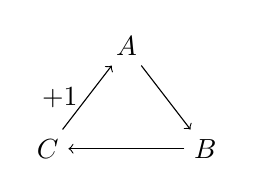
\begin{tikzpicture}[baseline=(current bounding box.center)]
      \node (A) at (1,1.3) {$A$}; \node (C) at (0,0)
      {$C$}; \node (B) at (2,0)
      {$B$}; \draw[->] (A) -- (B); \draw[->] (B) -- (C); \draw[->] (C)
      -- (A) node[midway, left] {$+1$};
    \end{tikzpicture}
  \]
  is a distinguished triangle in $\categ{K}(\categ{A})$ or
  $\categ{D}(\categ{A})$, then $\chi(B) = \chi(A) + \chi(C)$.
\end{exer}

\begin{exer}{\exerused{}}{exer:homol:9.2}
  Let $\categ{A}$ be an abelian category, and suppose two complexes
  $L^\bullet$, $M^\bullet$ are connected by an `upside-down roof' (a
  `trough'?)
  \[\begin{tikzcd}
      L^\bullet \arrow[dr] & & M^\bullet \arrow[dl,"\text{quasi-isomorphism}"] \\
      & N^\bullet &
    \end{tikzcd}\] Prove that they are also connected by a regular
  roof: there exists a complex $N^\bullet$ and morphisms
  $N^\bullet \to L^\bullet$ and $N^\bullet \to M^\bullet$ such that
  the diagram
  \[\begin{tikzcd}
      & N^\bullet \arrow[dl,"\text{quasi-isomorphism}"'] \arrow[dr] & \\
      L^\bullet \arrow[dr] & & M^\bullet \arrow[dl,"\text{quasi-isomorphism}"] \\
      & \underline{N}^\bullet &
    \end{tikzcd}\] commutes in $\categ{K}(\categ{A})$. Deduce that the
  composition of two roofs may be consolidated into a single roof in
  $\categ{K}(\categ{A})$. (Hint: Let
  $\alpha^\bullet : L^\bullet \to \underline{N}^\bullet$,
  $\beta^\bullet : M^\bullet \to \underline{N}^\bullet$ be the given
  morphisms, with $\beta^\bullet$ a quasi-isomorphism. Consider the
  composition
  $\gamma^\bullet : L^\bullet \to \underline{N}^\bullet \to
  MC(\beta)^\bullet$, and let $N^\bullet :=
  MC(\gamma)[-1]^\bullet$. We have
  $N^i = L^i \oplus M^i \oplus \underline{N}^{i-1}$, with morphisms to
  $L^i$, $M^i$ given, respectively, by $(\ell,m,n) \mapsto \ell$,
  $(\ell,m,n) \mapsto -m$; these define morphisms of cochain
  complexes. The morphisms $N^i \to \underline{N}^{i-1}$ defined by
  $(\ell,m,n) \mapsto -n$ define the homotopy showing that the diagram
  commutes in $\categ{K}(\categ{A})$. To verify that
  $N^\bullet \to L^\bullet$ is a quasi-isomorphism, use the fact that
  $MC(\beta)^\bullet$ is exact, and rotate a triangle.) [\S{}\ref{subsec:homol:derived-categories}]
\end{exer}

\begin{exer}{\exerused{}}{exer:homol:9.3}
  Let $\alpha^\bullet : L^\bullet \to M^\bullet$ be an isomorphism of
  cochain complexes. Prove that $MC(\alpha)^\bullet$ is homotopy
  equivalent to $0$. [\S{}\ref{subsec:homol:triangulated-categories}, \ref{exer:homol:9.4}]
\end{exer}

\begin{exer}{\exerused{}}{exer:homol:9.4}
  Let $\alpha^\bullet : L^\bullet \to M^\bullet$ be a cochain
  morphism, and let $\beta^\bullet : M^\bullet \to MC(\alpha)^\bullet$
  be the natural morphism. Prove that $MC(\beta)^\bullet$ is homotopy
  equivalent to $L[1]^\bullet$. (Hint: Do
  Exercise~\ref{exer:homol:9.3} first.) [\S{}\ref{subsec:homol:triangulated-categories}]
\end{exer}

\begin{exer}{\exerused{}}{exer:homol:9.5}
  Let
  \[
    0 \longrightarrow L^\bullet \xrightarrow{\alpha^\bullet} M^\bullet
    \xrightarrow{\beta^\bullet} N^\bullet \longrightarrow 0
  \]
  be a short exact sequence of cochain complexes on an abelian
  category.
  \begin{itemize}
  \item Prove that there is a cochain morphism
    $\gamma^\bullet : MC(\alpha)^\bullet \to N^\bullet$ through which
    $\beta^\bullet : M^\bullet \to N^\bullet$ factors.
  \item Prove that $MC(\gamma)^\bullet$ is an exact complex. (Hint:
    Chase elements.)
  \item Conclude that $MC(\alpha)^\bullet$ is quasi-isomorphic to
    $N^\bullet$.
  \end{itemize} [\S{}\ref{subsec:homol:triangulated-categories}]
\end{exer}

\begin{exer}{\exerused{}}{exer:homol:9.6}
  Let
  \[
    0 \longrightarrow L^\bullet \xrightarrow{\alpha^\bullet} M^\bullet
    \xrightarrow{\beta^\bullet} N^\bullet \longrightarrow 0
  \]
  be a short exact sequence of cochain complexes on an abelian
  category $\categ{A}$. Prove that there is a morphism
  $N^\bullet \to L[1]^\bullet$ in the derived category
  $\categ{D}(\categ{A})$, inducing the connecting morphism
  $H^i(N^\bullet) \to H^{i+1}(L^\bullet)$ in cohomology. [\S{}\ref{subsec:homol:triangulated-categories}]
\end{exer}

\begin{exer}{\exerused{}}{exer:homol:9.7}
  Prove Claim~\ref{fact:homol:9.1}. [\S{}\ref{subsec:homol:spectral-sequences}]
\end{exer}

\begin{exer}{\exerused{}}{exer:homol:9.8}
  Let $(E_r,d_r)_{r=1,2,\dots}$ be a spectral sequence arising from an
  exact couple
  \[
    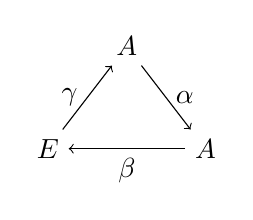
\begin{tikzpicture}[baseline=(current bounding box.center)]
      \node (A) at (1,1.3) {$A$}; \node (E) at (0,0)
      {$E$}; \node (A2) at (2,0)
      {$A$}; \draw[->] (A) -- (A2) node[midway, right]
      {$\alpha$}; \draw[->] (A2) -- (E) node[midway, below]
      {$\beta$}; \draw[->] (E) -- (A) node[midway, left] {$\gamma$};
    \end{tikzpicture}
  \]
  Prove that the limit $E_\infty$ is isomorphic to
  $\gamma^{-1}(\bigcap_r \image\alpha^r) / \beta(\bigcup_r
  \ker\alpha^r)$. (Hint: In fact,
  $Z_{r+1} = \gamma^{-1}(\image\alpha^r)$ and
  $B_{r+1} = \beta(\ker\alpha^r)$.) [\S{}\ref{subsec:homol:spectral-sequences}]
\end{exer}

\begin{exer}{}{exer:homol:9.9}
  Let ${}_vE_r$ be the spectral sequence of a first-quadrant double
  complex from the vertical filtration, as in \S{}9.3. Prove that
  ${}_vE_r^{i,j} = {}_vE_\infty^{i,j}$ for $r > j+1$.
\end{exer}

\begin{exer}{\exerused{}}{exer:homol:9.10}
  Let $\categ{A}$, $\categ{B}$, $\categ{C}$ be abelian categories, and
  let $\mathscr{F} : \categ{A} \to \categ{B}$,
  $\mathscr{G} : \categ{B} \to \categ{C}$ be additive functors. Assume
  that $\categ{A}$ and $\categ{B}$ have enough projectives, that
  $\mathscr{F}$ sends projectives of $\categ{A}$ to
  $\mathscr{G}$-acyclic objects of $\categ{B}$, and that $\mathscr{G}$
  is right-exact.

  Let $A$ be an object of $\categ{A}$, and let
  $M^\bullet : \dots \to M^{-2} \to M^{-1} \to M^0 \to 0$ be a
  projective resolution of $A$. Let $P_{\mathscr{F}M^\bullet}^\bullet$
  be a Cartan--Eilenberg resolution of the complex
  $\mathscr{F}M^\bullet$ (as constructed in \Cref{coro:homol:7.9}). Consider
  the complex
  \[
    (\dagger) \qquad \dots \longrightarrow
    \mathscr{G}(P_{\mathscr{F}M^{-2}}^\bullet) \longrightarrow
    \mathscr{G}(P_{\mathscr{F}M^{-1}}^\bullet) \longrightarrow
    \mathscr{G}(P_{\mathscr{F}M^0}^\bullet) \longrightarrow 0
  \]
  obtained by applying $\mathscr{G}$ to
  $P_{\mathscr{F}M^\bullet}^\bullet$.

  This is precisely the set-up of \Cref{exer:homol:8.8}. Now take the double
  complex associated with $(\dagger)$, and construct the spectral
  sequence corresponding to the horizontal filtration. Prove that the
  $E_2$ term of this sequence has terms
  \[ {}_hE_2^{p,q} =
    \categ{L}_p\mathscr{G}(\categ{L}_q\mathscr{F}(A)).
  \]
  (Use \Cref{exer:homol:7.6} to compute the ${}_hE_1$ term.)

  This is the Grothendieck spectral sequence mentioned at the end of
  \S{}9.3. Prove that it abuts to
  $\categ{L}_\bullet(\mathscr{G} \circ \mathscr{F})(A)$.

  (Use the `horizontal' version of Theorem~\ref{homol:9.5}, together
  with the computation of the cohomology of the total complex from
  \Cref{exer:homol:8.8}.) [\S{}\ref{subsec:homol:universal-property-of-the-derived-functor}, \ref{exer:homol:7.6}, \S{}\ref{subsec:homol:spectral-sequences}]
\end{exer}

%%% Local Variables:
%%% mode: LaTeX
%%% TeX-engine: luatex
%%% TeX-master: "../master"
%%% End:
